\documentclass{article}
\usepackage{amsmath}
\usepackage{color,pxfonts,fix-cm}
\usepackage{latexsym}
\usepackage[mathletters]{ucs}
\DeclareUnicodeCharacter{8211}{\textendash}
\DeclareUnicodeCharacter{34}{\textquotedbl}
\DeclareUnicodeCharacter{46}{\textperiodcentered}
\DeclareUnicodeCharacter{8220}{\textquotedblleft}
\DeclareUnicodeCharacter{8221}{\textquotedblright}
\DeclareUnicodeCharacter{58}{$\colon$}
\DeclareUnicodeCharacter{124}{\textbar}
\DeclareUnicodeCharacter{8226}{$\bullet$}
\DeclareUnicodeCharacter{9655}{$\triangleright$}
\DeclareUnicodeCharacter{191}{\textquestiondown}
\DeclareUnicodeCharacter{32}{$\ $}
\usepackage[T1]{fontenc}
\usepackage[utf8x]{inputenc}
\usepackage{pict2e}
\usepackage{wasysym}
\usepackage[english]{babel}
\usepackage{tikz}
\pagestyle{empty}
\usepackage[margin=0in,paperwidth=595pt,paperheight=841pt]{geometry}
\begin{document}
\definecolor{color_29791}{rgb}{0,0,0}
\definecolor{color_97849}{rgb}{0.266667,0.329412,0.415686}
\definecolor{color_283006}{rgb}{1,1,1}
\definecolor{color_80434}{rgb}{0.2,0.2,0.2}
\begin{tikzpicture}[overlay]\path(0pt,0pt);\end{tikzpicture}
\begin{picture}(-5,0)(2.5,0)
\put(79.464,-74.78003){\fontsize{15.96}{1}\usefont{T1}{cmr}{b}{n}\selectfont\color{color_29791}"Sistema Inteligente de Monitoreo y Control de Calidad del }
\put(205.25,-102.5){\fontsize{15.96}{1}\usefont{T1}{cmr}{b}{n}\selectfont\color{color_29791}Aire" SafeAir Monitor }
\put(96.14,-134.3){\fontsize{12}{1}\usefont{T1}{cmr}{m}{n}\selectfont\color{color_29791}Victor Molina}
\put(163.7,-129.74){\fontsize{8.04}{1}\usefont{T1}{cmr}{m}{n}\selectfont\color{color_29791}1}
\put(167.78,-134.3){\fontsize{12}{1}\usefont{T1}{cmr}{m}{n}\selectfont\color{color_29791}, Dennys Contreras}
\put(259.97,-129.74){\fontsize{8.04}{1}\usefont{T1}{cmr}{m}{n}\selectfont\color{color_29791}1}
\put(264.05,-134.3){\fontsize{12}{1}\usefont{T1}{cmr}{m}{n}\selectfont\color{color_29791}, William Vera}
\put(333.43,-129.74){\fontsize{8.04}{1}\usefont{T1}{cmr}{m}{n}\selectfont\color{color_29791}1}
\put(337.51,-134.3){\fontsize{12}{1}\usefont{T1}{cmr}{m}{n}\selectfont\color{color_29791}, Facultad de Ciencias de la }
\put(85.1,-155.06){\fontsize{12}{1}\usefont{T1}{cmr}{m}{n}\selectfont\color{color_29791}Ingeniería}
\put(133.58,-150.5){\fontsize{8.04}{1}\usefont{T1}{cmr}{m}{n}\selectfont\color{color_29791}1}
\put(137.66,-155.06){\fontsize{12}{1}\usefont{T1}{cmr}{m}{n}\selectfont\color{color_29791}, Universidad Técnica Estatal de Quevedo (UTEQ), Quevedo, Ecuador. }
\put(78.024,-181.7){\fontsize{11.04}{1}\usefont{T1}{cmr}{m}{n}\selectfont\color{color_29791}[victor.molina2017, dcontrerass, William.vera2018]@uteq.edu.ec }
\put(282.65,-209.66){\fontsize{11.04}{1}\usefont{T1}{cmr}{b}{n}\selectfont\color{color_29791} }
\put(70.104,-242.42){\fontsize{15.96}{1}\usefont{T1}{cmr}{b}{n}\selectfont\color{color_29791}Universidad Técnica Estatal de Quevedo - UTEQ }
\put(88.1,-286.01){\fontsize{14.04}{1}\usefont{T1}{cmr}{b}{n}\selectfont\color{color_29791}1. Introducción }
\put(70.104,-307.49){\fontsize{12}{1}\usefont{T1}{cmr}{m}{n}\selectfont\color{color_29791}En el ámbito cotidiano, nuestro hogar es un refugio de seguridad y bienestar, sin embargo, }
\put(70.104,-328.25){\fontsize{12}{1}\usefont{T1}{cmr}{m}{n}\selectfont\color{color_29791}no siempre estamos exentos de situaciones que puedan comprometer la salud de quienes }
\put(70.104,-348.89){\fontsize{12}{1}\usefont{T1}{cmr}{m}{n}\selectfont\color{color_29791}lo habitan. La calidad del aire en espacios interiores es un aspecto crítico, y los accidentes }
\put(70.104,-369.65){\fontsize{12}{1}\usefont{T1}{cmr}{m}{n}\selectfont\color{color_29791}domésticos pueden desencadenar eventos que ponen en peligro la pureza del aire, }
\put(70.104,-390.29){\fontsize{12}{1}\usefont{T1}{cmr}{m}{n}\selectfont\color{color_29791}especialmente para grupos vulnerables como niños, ancianos y personas con condiciones }
\put(70.104,-411.05){\fontsize{12}{1}\usefont{T1}{cmr}{m}{n}\selectfont\color{color_29791}médicas existentes. }
\put(70.104,-439.75){\fontsize{12}{1}\usefont{T1}{cmr}{m}{n}\selectfont\color{color_29791}Los incidentes domésticos, los cuales parecen inofensivos, pueden desencadenar la }
\put(70.104,-460.39){\fontsize{12}{1}\usefont{T1}{cmr}{m}{n}\selectfont\color{color_29791}liberación de sustancias nocivas en el ambiente interior. Desde pequeños escapes de gases }
\put(70.104,-481.15){\fontsize{12}{1}\usefont{T1}{cmr}{m}{n}\selectfont\color{color_29791}domésticos hasta la liberación de productos químicos durante tareas de limpieza, cada }
\put(70.104,-501.79){\fontsize{12}{1}\usefont{T1}{cmr}{m}{n}\selectfont\color{color_29791}uno de estos eventos tiene el potencial de afectar la calidad del aire que respiramos }
\put(70.104,-522.55){\fontsize{12}{1}\usefont{T1}{cmr}{m}{n}\selectfont\color{color_29791}diariamente. La magnitud de estos riesgos es aún más significativa cuando se considera }
\put(70.104,-543.19){\fontsize{12}{1}\usefont{T1}{cmr}{m}{n}\selectfont\color{color_29791}la vulnerabilidad de ciertos grupos de población, cuya salud puede estar más expuesta a }
\put(70.104,-563.95){\fontsize{12}{1}\usefont{T1}{cmr}{m}{n}\selectfont\color{color_29791}los impactos de la contaminación. }
\put(70.104,-592.63){\fontsize{12}{1}\usefont{T1}{cmr}{m}{n}\selectfont\color{color_29791}Este proyecto se concibe como una respuesta integral a esta problemática, explorando la }
\put(70.104,-613.42){\fontsize{12}{1}\usefont{T1}{cmr}{m}{n}\selectfont\color{color_29791}implementación de un "Sistema Inteligente de Monitoreo y Control de Calidad del Aire". }
\put(70.104,-634.06){\fontsize{12}{1}\usefont{T1}{cmr}{m}{n}\selectfont\color{color_29791}La iniciativa no solo se enfoca en la detección de contaminantes generados por accidentes }
\put(70.104,-654.7){\fontsize{12}{1}\usefont{T1}{cmr}{m}{n}\selectfont\color{color_29791}domésticos, sino que también busca tomar medidas automáticas para mitigar los riesgos }
\put(70.104,-675.46){\fontsize{12}{1}\usefont{T1}{cmr}{m}{n}\selectfont\color{color_29791}asociados, especialmente en áreas críticas donde la presencia de grupos vulnerables es }
\put(70.104,-696.1){\fontsize{12}{1}\usefont{T1}{cmr}{m}{n}\selectfont\color{color_29791}más acentuada. }
\put(70.104,-724.9){\fontsize{12}{1}\usefont{T1}{cmr}{m}{n}\selectfont\color{color_29791}A través de este enfoque proactivo, se aspira a mejorar las condiciones ambientales }
\put(70.104,-745.536){\fontsize{12}{1}\usefont{T1}{cmr}{m}{n}\selectfont\color{color_29791}internas, asegurando un ambiente seguro y saludable para todos los miembros del hogar. }
\end{picture}
\newpage
\begin{tikzpicture}[overlay]\path(0pt,0pt);\end{tikzpicture}
\begin{picture}(-5,0)(2.5,0)
\put(70.104,-71.03998){\fontsize{12}{1}\usefont{T1}{cmr}{m}{n}\selectfont\color{color_29791}Al abordar específicamente los riesgos derivados de accidentes domésticos, este proyecto }
\put(70.104,-91.82001){\fontsize{12}{1}\usefont{T1}{cmr}{m}{n}\selectfont\color{color_29791}busca no solo elevar la conciencia sobre la importancia de la calidad del aire en espacios }
\put(70.104,-112.46){\fontsize{12}{1}\usefont{T1}{cmr}{m}{n}\selectfont\color{color_29791}interiores, sino también proporcionar una solución innovadora para proteger a los más }
\put(70.104,-133.22){\fontsize{12}{1}\usefont{T1}{cmr}{m}{n}\selectfont\color{color_29791}vulnerables en nuestras comunidades. }
\put(88.1,-173.78){\fontsize{14.04}{1}\usefont{T1}{cmr}{b}{n}\selectfont\color{color_29791}2. Antecedentes }
\put(70.104,-195.26){\fontsize{12}{1}\usefont{T1}{cmr}{m}{n}\selectfont\color{color_29791}La calidad del aire en ambientes domésticos ha emergido como una preocupación crítica }
\put(70.104,-216.02){\fontsize{12}{1}\usefont{T1}{cmr}{m}{n}\selectfont\color{color_29791}debido a la variedad de factores que pueden comprometerla. Los accidentes domésticos, }
\put(70.104,-236.66){\fontsize{12}{1}\usefont{T1}{cmr}{m}{n}\selectfont\color{color_29791}que a menudo son pasados por alto, representan una fuente significativa de contaminación }
\put(70.104,-257.45){\fontsize{12}{1}\usefont{T1}{cmr}{m}{n}\selectfont\color{color_29791}del aire en espacios cerrados. Desde fugas de gases hasta la liberación inadvertida de }
\put(70.104,-278.09){\fontsize{12}{1}\usefont{T1}{cmr}{m}{n}\selectfont\color{color_29791}productos químicos tóxicos durante tareas cotidianas, estos eventos pueden afectar la }
\put(70.104,-298.85){\fontsize{12}{1}\usefont{T1}{cmr}{m}{n}\selectfont\color{color_29791}salud de los habitantes del hogar, especialmente aquellos pertenecientes a grupos }
\put(70.104,-319.49){\fontsize{12}{1}\usefont{T1}{cmr}{m}{n}\selectfont\color{color_29791}vulnerables como niños, ancianos y personas con condiciones médicas previas. }
\put(70.104,-348.17){\fontsize{12}{1}\usefont{T1}{cmr}{m}{n}\selectfont\color{color_29791}Las estadísticas revelan un aumento alarmante en los casos de enfermedades respiratorias }
\put(70.104,-368.93){\fontsize{12}{1}\usefont{T1}{cmr}{m}{n}\selectfont\color{color_29791}y problemas de salud relacionados con la calidad del aire en entornos interiores. Los }
\put(70.104,-389.57){\fontsize{12}{1}\usefont{T1}{cmr}{m}{n}\selectfont\color{color_29791}riesgos inherentes a los accidentes domésticos y su capacidad para desencadenar la }
\put(70.104,-410.33){\fontsize{12}{1}\usefont{T1}{cmr}{m}{n}\selectfont\color{color_29791}contaminación del aire plantean la necesidad apremiante de soluciones innovadoras que }
\put(70.104,-430.99){\fontsize{12}{1}\usefont{T1}{cmr}{m}{n}\selectfont\color{color_29791}aborden esta problemática desde una perspectiva proactiva. A pesar de los avances en la }
\put(70.104,-451.75){\fontsize{12}{1}\usefont{T1}{cmr}{m}{n}\selectfont\color{color_29791}conciencia ambiental, la mayoría de los sistemas de monitoreo de la calidad del aire se }
\put(70.104,-472.39){\fontsize{12}{1}\usefont{T1}{cmr}{m}{n}\selectfont\color{color_29791}centran en entornos exteriores, dejando un vacío significativo en la protección de la salud }
\put(70.104,-493.15){\fontsize{12}{1}\usefont{T1}{cmr}{m}{n}\selectfont\color{color_29791}en el hogar. Es en este contexto que surge la motivación para el desarrollo de un "Sistema }
\put(70.104,-513.79){\fontsize{12}{1}\usefont{T1}{cmr}{m}{n}\selectfont\color{color_29791}Inteligente de Monitoreo y Control de Calidad del Aire", destinado a abordar }
\put(70.104,-534.55){\fontsize{12}{1}\usefont{T1}{cmr}{m}{n}\selectfont\color{color_29791}específicamente los desafíos derivados de los accidentes domésticos y mejorar la calidad }
\put(70.104,-555.19){\fontsize{12}{1}\usefont{T1}{cmr}{m}{n}\selectfont\color{color_29791}del aire en el ambiente interior. Este proyecto se posiciona como una respuesta crucial }
\put(70.104,-575.95){\fontsize{12}{1}\usefont{T1}{cmr}{m}{n}\selectfont\color{color_29791}para mitigar los riesgos y crear hogares más seguros y saludables para todos. }
\put(88.1,-616.54){\fontsize{14.04}{1}\usefont{T1}{cmr}{b}{n}\selectfont\color{color_29791}3. Problema }
\put(70.104,-638.02){\fontsize{12}{1}\usefont{T1}{cmr}{m}{n}\selectfont\color{color_29791}La calidad del aire en espacios interiores es un aspecto crítico que puede afectar la salud }
\put(70.104,-658.66){\fontsize{12}{1}\usefont{T1}{cmr}{m}{n}\selectfont\color{color_29791}de las personas que habitan en ellos. Los accidentes domésticos, como pequeñas fugas de }
\put(70.104,-679.42){\fontsize{12}{1}\usefont{T1}{cmr}{m}{n}\selectfont\color{color_29791}gases o la liberación de productos químicos durante tareas cotidianas, pueden }
\put(70.104,-700.06){\fontsize{12}{1}\usefont{T1}{cmr}{m}{n}\selectfont\color{color_29791}comprometer la pureza del aire y poner en riesgo la salud de los habitantes, especialmente }
\put(70.104,-720.82){\fontsize{12}{1}\usefont{T1}{cmr}{m}{n}\selectfont\color{color_29791}de grupos vulnerables como niños, ancianos y personas con condiciones médicas }
\put(70.104,-741.456){\fontsize{12}{1}\usefont{T1}{cmr}{m}{n}\selectfont\color{color_29791}existentes. A pesar de los avances en la conciencia ambiental, la mayoría de los sistemas }
\end{picture}
\newpage
\begin{tikzpicture}[overlay]\path(0pt,0pt);\end{tikzpicture}
\begin{picture}(-5,0)(2.5,0)
\put(70.104,-71.03998){\fontsize{12}{1}\usefont{T1}{cmr}{m}{n}\selectfont\color{color_29791}de monitoreo de la calidad del aire se centran en entornos exteriores, dejando un vacío }
\put(70.104,-91.82001){\fontsize{12}{1}\usefont{T1}{cmr}{m}{n}\selectfont\color{color_29791}significativo en la protección de la salud en el hogar. Es en este contexto que surge la }
\put(70.104,-112.46){\fontsize{12}{1}\usefont{T1}{cmr}{m}{n}\selectfont\color{color_29791}necesidad de desarrollar un "Sistema Inteligente de Monitoreo y Control de Calidad del }
\put(70.104,-133.22){\fontsize{12}{1}\usefont{T1}{cmr}{m}{n}\selectfont\color{color_29791}Aire", destinado a detectar y prevenir la contaminación del aire en espacios interiores.  }
\put(88.1,-173.78){\fontsize{14.04}{1}\usefont{T1}{cmr}{b}{n}\selectfont\color{color_29791}4. Pregunta de investigación y objetivos }
\put(70.104,-195.26){\fontsize{12}{1}\usefont{T1}{cmr}{m}{n}\selectfont\color{color_29791}La pregunta de investigación que guio este estudio es: ¿Qué hacer en el caso de emisiones }
\put(70.104,-216.02){\fontsize{12}{1}\usefont{T1}{cmr}{m}{n}\selectfont\color{color_29791}de gases tóxicos y olores llenos de peligros? Esta pregunta surge a partir de la necesidad }
\put(70.104,-236.66){\fontsize{12}{1}\usefont{T1}{cmr}{m}{n}\selectfont\color{color_29791}de conocer el proceso a realizar luego de detectar problemas en el aire existentes. De tal }
\put(70.104,-257.45){\fontsize{12}{1}\usefont{T1}{cmr}{m}{n}\selectfont\color{color_29791}manera que permita plantear una solución viable que trate de reducir los problemas que }
\put(70.104,-278.09){\fontsize{12}{1}\usefont{T1}{cmr}{m}{n}\selectfont\color{color_29791}los sistemas existentes no resuelven. De esta pregunta de investigación se derivan los }
\put(70.104,-298.85){\fontsize{12}{1}\usefont{T1}{cmr}{m}{n}\selectfont\color{color_29791}siguientes objetivos }
\put(88.1,-339.41){\fontsize{14.04}{1}\usefont{T1}{cmr}{b}{n}\selectfont\color{color_29791}5. Pregunta de investigación y objetivos }
\put(70.104,-360.89){\fontsize{12}{1}\usefont{T1}{cmr}{m}{n}\selectfont\color{color_29791}La pregunta de investigación que guió este estudio es: ¿Cuáles son las características  }
\put(70.104,-389.57){\fontsize{12}{1}\usefont{T1}{cmr}{m}{n}\selectfont\color{color_29791}de los de Monitoreo y Control de Calidad del Aire que se han desarrollado hasta el }
\put(70.104,-410.21){\fontsize{12}{1}\usefont{T1}{cmr}{m}{n}\selectfont\color{color_29791}momento? Esta pregunta surge a partir de la necesidad de conocer el estado actual en }
\put(70.104,-430.99){\fontsize{12}{1}\usefont{T1}{cmr}{m}{n}\selectfont\color{color_29791}cuanto a las características de detección de calidad de aire existentes. De tal manera que }
\put(70.104,-451.63){\fontsize{12}{1}\usefont{T1}{cmr}{m}{n}\selectfont\color{color_29791}permita plantear una solución viable que trate de reducir las desventajas de los sistemas }
\put(70.104,-472.39){\fontsize{12}{1}\usefont{T1}{cmr}{m}{n}\selectfont\color{color_29791}existentes. De esta pregunta de investigación se derivan los siguientes objetivos. }
\put(88.1,-512.95){\fontsize{14.04}{1}\usefont{T1}{cmr}{b}{n}\selectfont\color{color_29791}6. Objetivos  }
\put(88.1,-536.35){\fontsize{14.04}{1}\usefont{T1}{cmr}{b}{n}\selectfont\color{color_29791}6.1. Objetivo General. }
\put(70.104,-551.83){\fontsize{12}{1}\usefont{T1}{cmr}{m}{n}\selectfont\color{color_29791}Desarrollar un sistema de Monitoreo y Control de Calidad del Aire buscando mejorar la }
\put(70.104,-572.47){\fontsize{12}{1}\usefont{T1}{cmr}{m}{n}\selectfont\color{color_29791}calidad y eficiencia de los sistemas tradicionales y mostrando nuestros propios modelos. }
\put(88.1,-603.19){\fontsize{14.04}{1}\usefont{T1}{cmr}{b}{n}\selectfont\color{color_29791}6.2. Objetivos Específicos. }
\put(70.104,-618.58){\fontsize{12}{1}\usefont{T1}{cmr}{m}{n}\selectfont\color{color_29791}• Realizar una revisión del estado del arte sobre los sistemas de Monitoreo y Control de }
\put(70.104,-639.34){\fontsize{12}{1}\usefont{T1}{cmr}{m}{n}\selectfont\color{color_29791}Calidad del Aire para identificar las limitaciones y oportunidades actuales. }
\put(70.104,-668.02){\fontsize{12}{1}\usefont{T1}{cmr}{m}{n}\selectfont\color{color_29791}• Recuperar datos de los trabajos presentados hasta el momento para analizar y verificar }
\put(70.104,-688.66){\fontsize{12}{1}\usefont{T1}{cmr}{m}{n}\selectfont\color{color_29791}la productividad que tienen los sistemas de detección }
\put(70.104,-717.46){\fontsize{12}{1}\usefont{T1}{cmr}{m}{n}\selectfont\color{color_29791}• Analizar los costos y beneficios del sistema de Monitoreo y Control de Calidad del Aire }
\put(70.104,-738.096){\fontsize{12}{1}\usefont{T1}{cmr}{m}{n}\selectfont\color{color_29791}en comparación con otros métodos de cultivo. }
\end{picture}
\newpage
\begin{tikzpicture}[overlay]\path(0pt,0pt);\end{tikzpicture}
\begin{picture}(-5,0)(2.5,0)
\put(88.1,-72.97998){\fontsize{14.04}{1}\usefont{T1}{cmr}{b}{n}\selectfont\color{color_29791}7. Solución  }
\put(70.104,-94.46002){\fontsize{12}{1}\usefont{T1}{cmr}{m}{n}\selectfont\color{color_29791}El Sistema Inteligente de Monitoreo y Control de Calidad del Aire “SafeAir Monitor” es }
\put(70.104,-115.22){\fontsize{12}{1}\usefont{T1}{cmr}{m}{n}\selectfont\color{color_29791}una solución innovadora y proactiva que busca garantizar la pureza del aire en espacios }
\put(70.104,-135.86){\fontsize{12}{1}\usefont{T1}{cmr}{m}{n}\selectfont\color{color_29791}interiores, especialmente para grupos vulnerables como niños, ancianos y personas con }
\put(70.104,-156.62){\fontsize{12}{1}\usefont{T1}{cmr}{m}{n}\selectfont\color{color_29791}condiciones médicas existentes. Este sistema utiliza sensores IoT para evaluar parámetros }
\put(70.104,-177.26){\fontsize{12}{1}\usefont{T1}{cmr}{m}{n}\selectfont\color{color_29791}como CO2, partículas suspendidas y compuestos orgánicos volátiles (COVs). }
\put(70.104,-205.94){\fontsize{12}{1}\usefont{T1}{cmr}{m}{n}\selectfont\color{color_29791}En caso de detectarse problemas con la calidad del aire, el sistema envía notificaciones a }
\put(70.104,-226.7){\fontsize{12}{1}\usefont{T1}{cmr}{m}{n}\selectfont\color{color_29791}los usuarios a través de una aplicación móvil, indicando la naturaleza del problema y las }
\put(70.104,-247.34){\fontsize{12}{1}\usefont{T1}{cmr}{m}{n}\selectfont\color{color_29791}medidas recomendadas para solucionarlo. Además, el sistema cuenta con una función de }
\put(70.104,-268.13){\fontsize{12}{1}\usefont{T1}{cmr}{m}{n}\selectfont\color{color_29791}ventilación automática que se activa en caso de detectarse niveles elevados de }
\put(70.104,-288.77){\fontsize{12}{1}\usefont{T1}{cmr}{m}{n}\selectfont\color{color_29791}contaminación, mejorando la calidad del aire en el ambiente interior. }
\put(70.104,-317.45){\fontsize{12}{1}\usefont{T1}{cmr}{m}{n}\selectfont\color{color_29791}La solución propuesta no solo se enfoca en la detección de contaminantes generados por }
\put(70.104,-338.21){\fontsize{12}{1}\usefont{T1}{cmr}{m}{n}\selectfont\color{color_29791}accidentes domésticos, sino que también busca tomar medidas automáticas para mitigar }
\put(70.104,-358.85){\fontsize{12}{1}\usefont{T1}{cmr}{m}{n}\selectfont\color{color_29791}los riesgos asociados, especialmente en áreas críticas donde la presencia de grupos }
\put(70.104,-379.61){\fontsize{12}{1}\usefont{T1}{cmr}{m}{n}\selectfont\color{color_29791}vulnerables es más acentuada. A través de este enfoque proactivo, se aspira a mejorar las }
\put(70.104,-400.25){\fontsize{12}{1}\usefont{T1}{cmr}{m}{n}\selectfont\color{color_29791}condiciones ambientales internas, asegurando un ambiente seguro y saludable para todos }
\put(70.104,-421.01){\fontsize{12}{1}\usefont{T1}{cmr}{m}{n}\selectfont\color{color_29791}los miembros del hogar. }
\put(88.1,-461.59){\fontsize{14.04}{1}\usefont{T1}{cmr}{b}{n}\selectfont\color{color_29791}8. Estudio del estado del arte }
\put(70.104,-483.07){\fontsize{12}{1}\usefont{T1}{cmr}{m}{n}\selectfont\color{color_29791}Presentamos los siguientes proyectos propuestos en el monitoreo de la calidad del aire en }
\put(70.104,-503.83){\fontsize{12}{1}\usefont{T1}{cmr}{m}{n}\selectfont\color{color_29791}hogares o espacios cerrados basados en el Internet de las Cosas (IoT). Gracias a la }
\put(70.104,-524.47){\fontsize{12}{1}\usefont{T1}{cmr}{m}{n}\selectfont\color{color_29791}búsqueda exhaustiva de literatura realizada, se ha recopilado una serie de estudios que }
\put(70.104,-545.23){\fontsize{12}{1}\usefont{T1}{cmr}{m}{n}\selectfont\color{color_29791}abordan estos avances tecnológicos. Estos trabajos fueron identificados mediante un }
\put(70.104,-565.87){\fontsize{12}{1}\usefont{T1}{cmr}{m}{n}\selectfont\color{color_29791}mapeo sistemático de la literatura, permitiendo encontrar investigaciones relevantes y }
\put(70.104,-586.51){\fontsize{12}{1}\usefont{T1}{cmr}{m}{n}\selectfont\color{color_29791}diversas.  }
\put(70.104,-615.34){\fontsize{12}{1}\usefont{T1}{cmr}{m}{n}\selectfont\color{color_29791}El trabajo presentado por Guerrero et al. [1], presenta a IdeAir como un sistema de }
\put(70.104,-635.98){\fontsize{12}{1}\usefont{T1}{cmr}{m}{n}\selectfont\color{color_29791}monitoreo de la calidad del aire en interiores. El objetivo es detectar concentraciones de }
\put(70.104,-656.74){\fontsize{12}{1}\usefont{T1}{cmr}{m}{n}\selectfont\color{color_29791}gases nocivos, emitiendo alarmas y activando medidas como encender el ventilador o }
\put(70.104,-677.38){\fontsize{12}{1}\usefont{T1}{cmr}{m}{n}\selectfont\color{color_29791}abrir la puerta. Utiliza sensores IoT para evaluar parámetros como CO2, partículas }
\put(70.104,-698.14){\fontsize{12}{1}\usefont{T1}{cmr}{m}{n}\selectfont\color{color_29791}suspendidas y compuestos orgánicos volátiles (COVs). Se emplea la metodología }
\put(70.104,-718.78){\fontsize{12}{1}\usefont{T1}{cmr}{m}{n}\selectfont\color{color_29791}TDDM4IoTS y tecnologías como Arduino IDE, Apache NetBeans IDE, Android Studio, }
\put(70.104,-739.536){\fontsize{12}{1}\usefont{T1}{cmr}{m}{n}\selectfont\color{color_29791}MySQL y WebHost. }
\end{picture}
\newpage
\begin{tikzpicture}[overlay]\path(0pt,0pt);\end{tikzpicture}
\begin{picture}(-5,0)(2.5,0)
\put(70.104,-71.03998){\fontsize{12}{1}\usefont{T1}{cmr}{m}{n}\selectfont\color{color_29791}El proyecto presentado por Alaa M \& Ishaq [2] I, se centra en fortalecer la seguridad en }
\put(70.104,-91.82001){\fontsize{12}{1}\usefont{T1}{cmr}{m}{n}\selectfont\color{color_29791}el hogar. Utiliza dispositivos de monitoreo de temperatura, detección de gas y humo, así }
\put(70.104,-112.46){\fontsize{12}{1}\usefont{T1}{cmr}{m}{n}\selectfont\color{color_29791}como un sistema de detección táctil. Emplea Microcontrolador ESP32, Arduino IDE, }
\put(70.104,-133.22){\fontsize{12}{1}\usefont{T1}{cmr}{m}{n}\selectfont\color{color_29791}ThingSpeak y Wireshark para implementar el sistema de seguridad. }
\put(70.104,-161.9){\fontsize{12}{1}\usefont{T1}{cmr}{m}{n}\selectfont\color{color_29791}La propuesta presentada por Pang L et al. [3] , se centra en un sistema de monitoreo de }
\put(70.104,-182.66){\fontsize{12}{1}\usefont{T1}{cmr}{m}{n}\selectfont\color{color_29791}calidad del aire en interiores (IAQMS) utilizando tecnología LoRa e IoT para medir CO2, }
\put(70.104,-203.3){\fontsize{12}{1}\usefont{T1}{cmr}{m}{n}\selectfont\color{color_29791}PM2.5, PM10, TVOC, HCHO, temperatura y humedad. Se enfoca en la selección de }
\put(70.104,-223.94){\fontsize{12}{1}\usefont{T1}{cmr}{m}{n}\selectfont\color{color_29791}hardware y sensores adecuados, el diseño de software y la integración con la plataforma }
\put(70.104,-244.7){\fontsize{12}{1}\usefont{T1}{cmr}{m}{n}\selectfont\color{color_29791}en la nube OneNET. }
\put(70.104,-273.41){\fontsize{12}{1}\usefont{T1}{cmr}{m}{n}\selectfont\color{color_29791}La investigación realizada por Zhou M et al. [4], realizó un sistema de monitoreo de }
\put(70.104,-294.17){\fontsize{12}{1}\usefont{T1}{cmr}{m}{n}\selectfont\color{color_29791}calidad del aire en interiores basado en IoT, utilizando Arduino Leonardo, sensores de }
\put(70.104,-314.81){\fontsize{12}{1}\usefont{T1}{cmr}{m}{n}\selectfont\color{color_29791}polvo, temperatura y humedad, The Things Network (TTN), Ubidots y el regulador de }
\put(70.104,-335.57){\fontsize{12}{1}\usefont{T1}{cmr}{m}{n}\selectfont\color{color_29791}voltaje LM317. }
\put(70.104,-364.25){\fontsize{12}{1}\usefont{T1}{cmr}{m}{n}\selectfont\color{color_29791}El trabajo propuesto por Rastogi K \& Lohani D [5] emplea sensores IoT para recopilar }
\put(70.104,-384.89){\fontsize{12}{1}\usefont{T1}{cmr}{m}{n}\selectfont\color{color_29791}datos sobre contaminantes del aire interior. Utiliza el Filtro de Kalman Extendido (EKF), }
\put(70.104,-405.65){\fontsize{12}{1}\usefont{T1}{cmr}{m}{n}\selectfont\color{color_29791}Sistema de Inferencia Neurodifuso Adaptativo (ANFIS), Cadenas de Markov Discretas }
\put(70.104,-426.29){\fontsize{12}{1}\usefont{T1}{cmr}{m}{n}\selectfont\color{color_29791}(DTMC), Amazon Web Services (AWS) y diversos sensores para procesar y predecir }
\put(70.104,-447.07){\fontsize{12}{1}\usefont{T1}{cmr}{m}{n}\selectfont\color{color_29791}cambios en la calidad del aire. }
\put(70.104,-475.75){\fontsize{12}{1}\usefont{T1}{cmr}{m}{n}\selectfont\color{color_29791}El estudio llevado a cabo por Pantelic J et al. [6], se enfoca en controlar las emisiones }
\put(70.104,-496.39){\fontsize{12}{1}\usefont{T1}{cmr}{m}{n}\selectfont\color{color_29791}generadas durante la cocina en hogares inteligentes. Evalúa algoritmos de control de }
\put(70.104,-517.15){\fontsize{12}{1}\usefont{T1}{cmr}{m}{n}\selectfont\color{color_29791}contaminación del aire utilizando sensores PM2.5, software StruxureWare, protocolo }
\put(70.104,-537.79){\fontsize{12}{1}\usefont{T1}{cmr}{m}{n}\selectfont\color{color_29791}BACnet, API de Sense, Azure y otras herramientas para el análisis de datos. }
\put(70.104,-566.47){\fontsize{12}{1}\usefont{T1}{cmr}{m}{n}\selectfont\color{color_29791}El estudio realizado por Wang J et al.  [7], se centra en la monitorización dinámica de la }
\put(70.104,-587.23){\fontsize{12}{1}\usefont{T1}{cmr}{m}{n}\selectfont\color{color_29791}contaminación del aire en interiores. Emplea sensores en tiempo real, algoritmos }
\put(70.104,-607.9){\fontsize{12}{1}\usefont{T1}{cmr}{m}{n}\selectfont\color{color_29791}predictivos y tecnologías de comunicación para anticipar cambios en la calidad del aire y }
\put(70.104,-628.66){\fontsize{12}{1}\usefont{T1}{cmr}{m}{n}\selectfont\color{color_29791}proporcionar alertas y recomendaciones. }
\put(70.104,-657.34){\fontsize{12}{1}\usefont{T1}{cmr}{m}{n}\selectfont\color{color_29791}Después de realizar una revisión exhaustiva de los trabajos recopilados, se procedió a }
\put(70.104,-678.1){\fontsize{12}{1}\usefont{T1}{cmr}{m}{n}\selectfont\color{color_29791}categorizarlos para destacar sus enfoques y contribuciones específicas: }
\put(70.104,-706.78){\fontsize{12}{1}\usefont{T1}{cmr}{m}{n}\selectfont\color{color_29791}Un conjunto de trabajos, J. M. Corchado et al. [1], L. Pang et al. [3], M. Zhou et al. [4] y }
\put(70.104,-727.42){\fontsize{12}{1}\usefont{T1}{cmr}{m}{n}\selectfont\color{color_29791}J. Wang et al. [7], se centran en el desarrollo de sistemas de monitoreo destinados a }
\put(70.104,-748.176){\fontsize{12}{1}\usefont{T1}{cmr}{m}{n}\selectfont\color{color_29791}mejorar la calidad del aire en entornos interiores. Estos proyectos emplean una amplia }
\end{picture}
\newpage
\begin{tikzpicture}[overlay]\path(0pt,0pt);\end{tikzpicture}
\begin{picture}(-5,0)(2.5,0)
\put(70.104,-71.03998){\fontsize{12}{1}\usefont{T1}{cmr}{m}{n}\selectfont\color{color_29791}variedad de sensores y plataformas IoT, abordando parámetros esenciales como CO2, }
\put(70.104,-91.82001){\fontsize{12}{1}\usefont{T1}{cmr}{m}{n}\selectfont\color{color_29791}partículas suspendidas, temperatura y humedad. Su principal objetivo es ofrecer }
\put(70.104,-112.46){\fontsize{12}{1}\usefont{T1}{cmr}{m}{n}\selectfont\color{color_29791}soluciones integrales para garantizar entornos interiores más saludables y seguros. }
\put(70.104,-141.26){\fontsize{12}{1}\usefont{T1}{cmr}{m}{n}\selectfont\color{color_29791}En contraste, A. M. Odeh and I. Ishaq [2] y K. Rastogi and D. Lohani [5] tienen una }
\put(70.104,-161.9){\fontsize{12}{1}\usefont{T1}{cmr}{m}{n}\selectfont\color{color_29791}orientación más específica hacia la seguridad en el hogar. Ambos trabajos destacan la }
\put(70.104,-182.66){\fontsize{12}{1}\usefont{T1}{cmr}{m}{n}\selectfont\color{color_29791}detección de gas, humo y temperatura para fortalecer la protección en entornos }
\put(70.104,-203.3){\fontsize{12}{1}\usefont{T1}{cmr}{m}{n}\selectfont\color{color_29791}domésticos. K. Rastogi and D. Lohani [5] se distingue por emplear algoritmos para }
\put(70.104,-223.94){\fontsize{12}{1}\usefont{T1}{cmr}{m}{n}\selectfont\color{color_29791}procesar datos de sensores y estimar valores faltantes en la calidad del aire interior, }
\put(70.104,-244.7){\fontsize{12}{1}\usefont{T1}{cmr}{m}{n}\selectfont\color{color_29791}mientras que A. M. Odeh and I. Ishaq [2] se centra en la instalación estratégica de }
\put(70.104,-265.37){\fontsize{12}{1}\usefont{T1}{cmr}{m}{n}\selectfont\color{color_29791}dispositivos de monitoreo para el hogar inteligente. }
\put(70.104,-294.17){\fontsize{12}{1}\usefont{T1}{cmr}{m}{n}\selectfont\color{color_29791}Por otro lado, J. Pantelic et al. [6] se enfoca en controlar las emisiones generadas durante }
\put(70.104,-314.81){\fontsize{12}{1}\usefont{T1}{cmr}{m}{n}\selectfont\color{color_29791}la cocción en hogares inteligentes, evaluando algoritmos diseñados para reducir la }
\put(70.104,-335.57){\fontsize{12}{1}\usefont{T1}{cmr}{m}{n}\selectfont\color{color_29791}contaminación del aire asociada con este proceso específico. }
\put(70.104,-364.25){\fontsize{12}{1}\usefont{T1}{cmr}{m}{n}\selectfont\color{color_29791}Además, es relevante destacar que J. M. Corchado et al. [1], M. Zhou et al. [4] y K. }
\put(70.104,-384.89){\fontsize{12}{1}\usefont{T1}{cmr}{m}{n}\selectfont\color{color_29791}Rastogi and D. Lohani [5] incorporan sistemas de notificaciones o alertas destinados a }
\put(70.104,-405.65){\fontsize{12}{1}\usefont{T1}{cmr}{m}{n}\selectfont\color{color_29791}informar a los usuarios sobre la calidad del aire o posibles riesgos detectados. En }
\put(70.104,-426.29){\fontsize{12}{1}\usefont{T1}{cmr}{m}{n}\selectfont\color{color_29791}contraste, A. M. Odeh and I. Ishaq [2], L. Pang et al. [3], J. Pantelic et al. [6] y J. Wang }
\put(70.104,-447.07){\fontsize{12}{1}\usefont{T1}{cmr}{m}{n}\selectfont\color{color_29791}et al. [7] no especifican explícitamente si proporcionan esta funcionalidad, lo que resalta }
\put(70.104,-467.71){\fontsize{12}{1}\usefont{T1}{cmr}{m}{n}\selectfont\color{color_29791}la diversidad de características entre los proyectos analizados. }
\put(70.104,-496.39){\fontsize{12}{1}\usefont{T1}{cmr}{m}{n}\selectfont\color{color_29791} }
\put(177.29,-522.43){\fontsize{9}{1}\usefont{T1}{cmr}{m}{it}\selectfont\color{color_29791}Tabla 1. Trabajos rescatados de la búsqueda de literatura. }
\put(79.704,-551.35){\fontsize{10.56}{1}\usefont{T1}{cmr}{b}{n}\selectfont\color{color_29791}Nombre del }
\put(90.38,-572.35){\fontsize{10.56}{1}\usefont{T1}{cmr}{b}{n}\selectfont\color{color_29791}Trabajo }
\put(164.06,-551.35){\fontsize{10.56}{1}\usefont{T1}{cmr}{b}{n}\selectfont\color{color_29791}Proyecto }
\put(158.18,-572.35){\fontsize{10.56}{1}\usefont{T1}{cmr}{b}{n}\selectfont\color{color_29791}Presentado }
\put(229.61,-551.35){\fontsize{10.56}{1}\usefont{T1}{cmr}{b}{n}\selectfont\color{color_29791}Tipos de Aire }
\put(231.05,-572.35){\fontsize{10.56}{1}\usefont{T1}{cmr}{b}{n}\selectfont\color{color_29791}Reconocidos }
\put(308.95,-551.35){\fontsize{10.56}{1}\usefont{T1}{cmr}{b}{n}\selectfont\color{color_29791}Herramientas }
\put(318.31,-572.35){\fontsize{10.56}{1}\usefont{T1}{cmr}{b}{n}\selectfont\color{color_29791}Utilizadas }
\put(389.95,-551.35){\fontsize{10.56}{1}\usefont{T1}{cmr}{b}{n}\selectfont\color{color_29791}Notificaciones/Alert}
\put(434.62,-572.35){\fontsize{10.56}{1}\usefont{T1}{cmr}{b}{n}\selectfont\color{color_29791}as }
\end{picture}
\begin{tikzpicture}[overlay]
\path(0pt,0pt);
\filldraw[color_29791][even odd rule]
(70.104pt, -539.95pt) -- (70.584pt, -539.95pt)
 -- (70.584pt, -539.95pt)
 -- (70.584pt, -539.47pt)
 -- (70.584pt, -539.47pt)
 -- (70.104pt, -539.47pt) -- cycle
;
\filldraw[color_29791][even odd rule]
(70.104pt, -539.95pt) -- (70.584pt, -539.95pt)
 -- (70.584pt, -539.95pt)
 -- (70.584pt, -539.47pt)
 -- (70.584pt, -539.47pt)
 -- (70.104pt, -539.47pt) -- cycle
;
\filldraw[color_29791][even odd rule]
(70.584pt, -539.95pt) -- (147.744pt, -539.95pt)
 -- (147.744pt, -539.95pt)
 -- (147.744pt, -539.47pt)
 -- (147.744pt, -539.47pt)
 -- (70.584pt, -539.47pt) -- cycle
;
\filldraw[color_29791][even odd rule]
(147.74pt, -539.95pt) -- (148.22pt, -539.95pt)
 -- (148.22pt, -539.95pt)
 -- (148.22pt, -539.47pt)
 -- (148.22pt, -539.47pt)
 -- (147.74pt, -539.47pt) -- cycle
;
\filldraw[color_29791][even odd rule]
(148.22pt, -539.95pt) -- (223.844pt, -539.95pt)
 -- (223.844pt, -539.95pt)
 -- (223.844pt, -539.47pt)
 -- (223.844pt, -539.47pt)
 -- (148.22pt, -539.47pt) -- cycle
;
\filldraw[color_29791][even odd rule]
(223.85pt, -539.95pt) -- (224.33pt, -539.95pt)
 -- (224.33pt, -539.95pt)
 -- (224.33pt, -539.47pt)
 -- (224.33pt, -539.47pt)
 -- (223.85pt, -539.47pt) -- cycle
;
\filldraw[color_29791][even odd rule]
(224.33pt, -539.95pt) -- (300.194pt, -539.95pt)
 -- (300.194pt, -539.95pt)
 -- (300.194pt, -539.47pt)
 -- (300.194pt, -539.47pt)
 -- (224.33pt, -539.47pt) -- cycle
;
\filldraw[color_29791][even odd rule]
(300.19pt, -539.95pt) -- (300.67pt, -539.95pt)
 -- (300.67pt, -539.95pt)
 -- (300.67pt, -539.47pt)
 -- (300.67pt, -539.47pt)
 -- (300.19pt, -539.47pt) -- cycle
;
\filldraw[color_29791][even odd rule]
(300.67pt, -539.95pt) -- (384.31pt, -539.95pt)
 -- (384.31pt, -539.95pt)
 -- (384.31pt, -539.47pt)
 -- (384.31pt, -539.47pt)
 -- (300.67pt, -539.47pt) -- cycle
;
\filldraw[color_29791][even odd rule]
(384.31pt, -539.95pt) -- (384.79pt, -539.95pt)
 -- (384.79pt, -539.95pt)
 -- (384.79pt, -539.47pt)
 -- (384.79pt, -539.47pt)
 -- (384.31pt, -539.47pt) -- cycle
;
\filldraw[color_29791][even odd rule]
(384.79pt, -539.95pt) -- (494.85pt, -539.95pt)
 -- (494.85pt, -539.95pt)
 -- (494.85pt, -539.47pt)
 -- (494.85pt, -539.47pt)
 -- (384.79pt, -539.47pt) -- cycle
;
\filldraw[color_29791][even odd rule]
(494.86pt, -539.95pt) -- (495.34pt, -539.95pt)
 -- (495.34pt, -539.95pt)
 -- (495.34pt, -539.47pt)
 -- (495.34pt, -539.47pt)
 -- (494.86pt, -539.47pt) -- cycle
;
\filldraw[color_29791][even odd rule]
(494.86pt, -539.95pt) -- (495.34pt, -539.95pt)
 -- (495.34pt, -539.95pt)
 -- (495.34pt, -539.47pt)
 -- (495.34pt, -539.47pt)
 -- (494.86pt, -539.47pt) -- cycle
;
\filldraw[color_29791][even odd rule]
(70.104pt, -581.83pt) -- (70.584pt, -581.83pt)
 -- (70.584pt, -581.83pt)
 -- (70.584pt, -539.95pt)
 -- (70.584pt, -539.95pt)
 -- (70.104pt, -539.95pt) -- cycle
;
\filldraw[color_29791][even odd rule]
(147.74pt, -581.83pt) -- (148.22pt, -581.83pt)
 -- (148.22pt, -581.83pt)
 -- (148.22pt, -539.95pt)
 -- (148.22pt, -539.95pt)
 -- (147.74pt, -539.95pt) -- cycle
;
\filldraw[color_29791][even odd rule]
(223.85pt, -581.83pt) -- (224.33pt, -581.83pt)
 -- (224.33pt, -581.83pt)
 -- (224.33pt, -539.95pt)
 -- (224.33pt, -539.95pt)
 -- (223.85pt, -539.95pt) -- cycle
;
\filldraw[color_29791][even odd rule]
(300.19pt, -581.83pt) -- (300.67pt, -581.83pt)
 -- (300.67pt, -581.83pt)
 -- (300.67pt, -539.95pt)
 -- (300.67pt, -539.95pt)
 -- (300.19pt, -539.95pt) -- cycle
;
\filldraw[color_29791][even odd rule]
(384.31pt, -581.83pt) -- (384.79pt, -581.83pt)
 -- (384.79pt, -581.83pt)
 -- (384.79pt, -539.95pt)
 -- (384.79pt, -539.95pt)
 -- (384.31pt, -539.95pt) -- cycle
;
\filldraw[color_29791][even odd rule]
(494.86pt, -581.83pt) -- (495.34pt, -581.83pt)
 -- (495.34pt, -581.83pt)
 -- (495.34pt, -539.95pt)
 -- (495.34pt, -539.95pt)
 -- (494.86pt, -539.95pt) -- cycle
;
\begin{scope}
\clip
(70.584pt, -729.1pt) -- (147.624pt, -729.1pt)
 -- (147.624pt, -729.1pt)
 -- (147.624pt, -582.44pt)
 -- (147.624pt, -582.44pt)
 -- (70.584pt, -582.44pt) -- cycle
;
\begin{scope}
\clip
(70.584pt, -729.1pt) -- (147.624pt, -729.1pt)
 -- (147.624pt, -729.1pt)
 -- (147.624pt, -582.44pt)
 -- (147.624pt, -582.44pt)
 -- (70.584pt, -582.44pt) -- cycle
;
\end{scope}
\end{scope}
\end{tikzpicture}
\begin{picture}(-5,0)(2.5,0)
\put(75.744,-593.83){\fontsize{10.56}{1}\usefont{T1}{cmr}{m}{n}\selectfont\color{color_29791}The }
\put(75.744,-614.74){\fontsize{10.56}{1}\usefont{T1}{cmr}{m}{n}\selectfont\color{color_29791}Implementati}
\put(75.744,-635.74){\fontsize{10.56}{1}\usefont{T1}{cmr}{m}{n}\selectfont\color{color_29791}on of a Smart }
\put(75.744,-656.62){\fontsize{10.56}{1}\usefont{T1}{cmr}{m}{n}\selectfont\color{color_29791}Home }
\put(75.744,-677.62){\fontsize{10.56}{1}\usefont{T1}{cmr}{m}{n}\selectfont\color{color_29791}Security }
\put(75.744,-698.5){\fontsize{10.56}{1}\usefont{T1}{cmr}{m}{n}\selectfont\color{color_29791}Network }
\put(75.744,-719.5){\fontsize{10.56}{1}\usefont{T1}{cmr}{m}{n}\selectfont\color{color_29791}Using Internet }
\put(154.94,-625.18){\fontsize{10.56}{1}\usefont{T1}{cmr}{m}{n}\selectfont\color{color_29791}Fortalecimien}
\put(168.5,-646.18){\fontsize{10.56}{1}\usefont{T1}{cmr}{m}{n}\selectfont\color{color_29791}to de la }
\put(155.3,-667.18){\fontsize{10.56}{1}\usefont{T1}{cmr}{m}{n}\selectfont\color{color_29791}Seguridad en }
\put(166.22,-688.06){\fontsize{10.56}{1}\usefont{T1}{cmr}{m}{n}\selectfont\color{color_29791}el Hogar }
\put(231.41,-646.18){\fontsize{10.56}{1}\usefont{T1}{cmr}{m}{n}\selectfont\color{color_29791}Temperatura, }
\put(236.81,-667.18){\fontsize{10.56}{1}\usefont{T1}{cmr}{m}{n}\selectfont\color{color_29791}Gas, Humo }
\put(306.91,-593.83){\fontsize{10.56}{1}\usefont{T1}{cmr}{m}{n}\selectfont\color{color_29791}Microcontrolad}
\put(320.83,-614.74){\fontsize{10.56}{1}\usefont{T1}{cmr}{m}{n}\selectfont\color{color_29791}or ESP32, }
\put(320.59,-635.74){\fontsize{10.56}{1}\usefont{T1}{cmr}{m}{n}\selectfont\color{color_29791}Sensores, }
\put(314.95,-656.62){\fontsize{10.56}{1}\usefont{T1}{cmr}{m}{n}\selectfont\color{color_29791}Actuadores, }
\put(313.39,-677.62){\fontsize{10.56}{1}\usefont{T1}{cmr}{m}{n}\selectfont\color{color_29791}Arduino IDE, }
\put(314.23,-698.5){\fontsize{10.56}{1}\usefont{T1}{cmr}{m}{n}\selectfont\color{color_29791}ThingSpeak, }
\put(319.39,-719.5){\fontsize{10.56}{1}\usefont{T1}{cmr}{m}{n}\selectfont\color{color_29791}Wireshark }
\put(435.7,-656.62){\fontsize{10.56}{1}\usefont{T1}{cmr}{m}{n}\selectfont\color{color_29791}Sí }
\end{picture}
\begin{tikzpicture}[overlay]
\path(0pt,0pt);
\filldraw[color_29791][even odd rule]
(70.104pt, -582.31pt) -- (70.584pt, -582.31pt)
 -- (70.584pt, -582.31pt)
 -- (70.584pt, -581.83pt)
 -- (70.584pt, -581.83pt)
 -- (70.104pt, -581.83pt) -- cycle
;
\filldraw[color_29791][even odd rule]
(70.584pt, -582.31pt) -- (147.744pt, -582.31pt)
 -- (147.744pt, -582.31pt)
 -- (147.744pt, -581.83pt)
 -- (147.744pt, -581.83pt)
 -- (70.584pt, -581.83pt) -- cycle
;
\filldraw[color_29791][even odd rule]
(147.74pt, -582.31pt) -- (148.22pt, -582.31pt)
 -- (148.22pt, -582.31pt)
 -- (148.22pt, -581.83pt)
 -- (148.22pt, -581.83pt)
 -- (147.74pt, -581.83pt) -- cycle
;
\filldraw[color_29791][even odd rule]
(148.22pt, -582.31pt) -- (223.844pt, -582.31pt)
 -- (223.844pt, -582.31pt)
 -- (223.844pt, -581.83pt)
 -- (223.844pt, -581.83pt)
 -- (148.22pt, -581.83pt) -- cycle
;
\filldraw[color_29791][even odd rule]
(223.85pt, -582.31pt) -- (224.33pt, -582.31pt)
 -- (224.33pt, -582.31pt)
 -- (224.33pt, -581.83pt)
 -- (224.33pt, -581.83pt)
 -- (223.85pt, -581.83pt) -- cycle
;
\filldraw[color_29791][even odd rule]
(224.33pt, -582.31pt) -- (300.194pt, -582.31pt)
 -- (300.194pt, -582.31pt)
 -- (300.194pt, -581.83pt)
 -- (300.194pt, -581.83pt)
 -- (224.33pt, -581.83pt) -- cycle
;
\filldraw[color_29791][even odd rule]
(300.19pt, -582.31pt) -- (300.67pt, -582.31pt)
 -- (300.67pt, -582.31pt)
 -- (300.67pt, -581.83pt)
 -- (300.67pt, -581.83pt)
 -- (300.19pt, -581.83pt) -- cycle
;
\filldraw[color_29791][even odd rule]
(300.67pt, -582.31pt) -- (384.31pt, -582.31pt)
 -- (384.31pt, -582.31pt)
 -- (384.31pt, -581.83pt)
 -- (384.31pt, -581.83pt)
 -- (300.67pt, -581.83pt) -- cycle
;
\filldraw[color_29791][even odd rule]
(384.31pt, -582.31pt) -- (384.79pt, -582.31pt)
 -- (384.79pt, -582.31pt)
 -- (384.79pt, -581.83pt)
 -- (384.79pt, -581.83pt)
 -- (384.31pt, -581.83pt) -- cycle
;
\filldraw[color_29791][even odd rule]
(384.79pt, -582.31pt) -- (494.85pt, -582.31pt)
 -- (494.85pt, -582.31pt)
 -- (494.85pt, -581.83pt)
 -- (494.85pt, -581.83pt)
 -- (384.79pt, -581.83pt) -- cycle
;
\filldraw[color_29791][even odd rule]
(494.86pt, -582.31pt) -- (495.34pt, -582.31pt)
 -- (495.34pt, -582.31pt)
 -- (495.34pt, -581.83pt)
 -- (495.34pt, -581.83pt)
 -- (494.86pt, -581.83pt) -- cycle
;
\filldraw[color_29791][even odd rule]
(70.104pt, -729.1pt) -- (70.584pt, -729.1pt)
 -- (70.584pt, -729.1pt)
 -- (70.584pt, -582.32pt)
 -- (70.584pt, -582.32pt)
 -- (70.104pt, -582.32pt) -- cycle
;
\filldraw[color_29791][even odd rule]
(70.104pt, -729.58pt) -- (70.584pt, -729.58pt)
 -- (70.584pt, -729.58pt)
 -- (70.584pt, -729.1pt)
 -- (70.584pt, -729.1pt)
 -- (70.104pt, -729.1pt) -- cycle
;
\filldraw[color_29791][even odd rule]
(70.104pt, -729.58pt) -- (70.584pt, -729.58pt)
 -- (70.584pt, -729.58pt)
 -- (70.584pt, -729.1pt)
 -- (70.584pt, -729.1pt)
 -- (70.104pt, -729.1pt) -- cycle
;
\filldraw[color_29791][even odd rule]
(70.584pt, -729.58pt) -- (147.744pt, -729.58pt)
 -- (147.744pt, -729.58pt)
 -- (147.744pt, -729.1pt)
 -- (147.744pt, -729.1pt)
 -- (70.584pt, -729.1pt) -- cycle
;
\filldraw[color_29791][even odd rule]
(147.74pt, -729.1pt) -- (148.22pt, -729.1pt)
 -- (148.22pt, -729.1pt)
 -- (148.22pt, -582.32pt)
 -- (148.22pt, -582.32pt)
 -- (147.74pt, -582.32pt) -- cycle
;
\filldraw[color_29791][even odd rule]
(147.74pt, -729.58pt) -- (148.22pt, -729.58pt)
 -- (148.22pt, -729.58pt)
 -- (148.22pt, -729.1pt)
 -- (148.22pt, -729.1pt)
 -- (147.74pt, -729.1pt) -- cycle
;
\filldraw[color_29791][even odd rule]
(148.22pt, -729.58pt) -- (223.844pt, -729.58pt)
 -- (223.844pt, -729.58pt)
 -- (223.844pt, -729.1pt)
 -- (223.844pt, -729.1pt)
 -- (148.22pt, -729.1pt) -- cycle
;
\filldraw[color_29791][even odd rule]
(223.85pt, -729.1pt) -- (224.33pt, -729.1pt)
 -- (224.33pt, -729.1pt)
 -- (224.33pt, -582.32pt)
 -- (224.33pt, -582.32pt)
 -- (223.85pt, -582.32pt) -- cycle
;
\filldraw[color_29791][even odd rule]
(223.85pt, -729.58pt) -- (224.33pt, -729.58pt)
 -- (224.33pt, -729.58pt)
 -- (224.33pt, -729.1pt)
 -- (224.33pt, -729.1pt)
 -- (223.85pt, -729.1pt) -- cycle
;
\filldraw[color_29791][even odd rule]
(224.33pt, -729.58pt) -- (300.194pt, -729.58pt)
 -- (300.194pt, -729.58pt)
 -- (300.194pt, -729.1pt)
 -- (300.194pt, -729.1pt)
 -- (224.33pt, -729.1pt) -- cycle
;
\filldraw[color_29791][even odd rule]
(300.19pt, -729.1pt) -- (300.67pt, -729.1pt)
 -- (300.67pt, -729.1pt)
 -- (300.67pt, -582.32pt)
 -- (300.67pt, -582.32pt)
 -- (300.19pt, -582.32pt) -- cycle
;
\filldraw[color_29791][even odd rule]
(300.19pt, -729.58pt) -- (300.67pt, -729.58pt)
 -- (300.67pt, -729.58pt)
 -- (300.67pt, -729.1pt)
 -- (300.67pt, -729.1pt)
 -- (300.19pt, -729.1pt) -- cycle
;
\filldraw[color_29791][even odd rule]
(300.67pt, -729.58pt) -- (384.31pt, -729.58pt)
 -- (384.31pt, -729.58pt)
 -- (384.31pt, -729.1pt)
 -- (384.31pt, -729.1pt)
 -- (300.67pt, -729.1pt) -- cycle
;
\filldraw[color_29791][even odd rule]
(384.31pt, -729.1pt) -- (384.79pt, -729.1pt)
 -- (384.79pt, -729.1pt)
 -- (384.79pt, -582.32pt)
 -- (384.79pt, -582.32pt)
 -- (384.31pt, -582.32pt) -- cycle
;
\filldraw[color_29791][even odd rule]
(384.31pt, -729.58pt) -- (384.79pt, -729.58pt)
 -- (384.79pt, -729.58pt)
 -- (384.79pt, -729.1pt)
 -- (384.79pt, -729.1pt)
 -- (384.31pt, -729.1pt) -- cycle
;
\filldraw[color_29791][even odd rule]
(384.79pt, -729.58pt) -- (494.85pt, -729.58pt)
 -- (494.85pt, -729.58pt)
 -- (494.85pt, -729.1pt)
 -- (494.85pt, -729.1pt)
 -- (384.79pt, -729.1pt) -- cycle
;
\filldraw[color_29791][even odd rule]
(494.86pt, -729.1pt) -- (495.34pt, -729.1pt)
 -- (495.34pt, -729.1pt)
 -- (495.34pt, -582.32pt)
 -- (495.34pt, -582.32pt)
 -- (494.86pt, -582.32pt) -- cycle
;
\filldraw[color_29791][even odd rule]
(494.86pt, -729.58pt) -- (495.34pt, -729.58pt)
 -- (495.34pt, -729.58pt)
 -- (495.34pt, -729.1pt)
 -- (495.34pt, -729.1pt)
 -- (494.86pt, -729.1pt) -- cycle
;
\end{tikzpicture}
\newpage
\begin{tikzpicture}[overlay]
\path(0pt,0pt);
\filldraw[color_29791][even odd rule]
(494.86pt, -729.58pt) -- (495.34pt, -729.58pt)
 -- (495.34pt, -729.58pt)
 -- (495.34pt, -729.1pt)
 -- (495.34pt, -729.1pt)
 -- (494.86pt, -729.1pt) -- cycle
;
\begin{scope}
\clip
(70.584pt, -102.38pt) -- (147.624pt, -102.38pt)
 -- (147.624pt, -102.38pt)
 -- (147.624pt, -60.47601pt)
 -- (147.624pt, -60.47601pt)
 -- (70.584pt, -60.47601pt) -- cycle
;
\begin{scope}
\clip
(70.584pt, -102.38pt) -- (147.624pt, -102.38pt)
 -- (147.624pt, -102.38pt)
 -- (147.624pt, -60.47601pt)
 -- (147.624pt, -60.47601pt)
 -- (70.584pt, -60.47601pt) -- cycle
;
\end{scope}
\end{scope}
\end{tikzpicture}
\begin{picture}(-5,0)(2.5,0)
\put(75.744,-71.88){\fontsize{10.56}{1}\usefont{T1}{cmr}{m}{n}\selectfont\color{color_29791}of Things (IoT) }
\put(75.744,-92.78003){\fontsize{10.56}{1}\usefont{T1}{cmr}{m}{n}\selectfont\color{color_29791}System }
\end{picture}
\begin{tikzpicture}[overlay]
\path(0pt,0pt);
\filldraw[color_29791][even odd rule]
(70.104pt, -60.35999pt) -- (70.584pt, -60.35999pt)
 -- (70.584pt, -60.35999pt)
 -- (70.584pt, -59.88pt)
 -- (70.584pt, -59.88pt)
 -- (70.104pt, -59.88pt) -- cycle
;
\filldraw[color_29791][even odd rule]
(70.104pt, -60.35999pt) -- (70.584pt, -60.35999pt)
 -- (70.584pt, -60.35999pt)
 -- (70.584pt, -59.88pt)
 -- (70.584pt, -59.88pt)
 -- (70.104pt, -59.88pt) -- cycle
;
\filldraw[color_29791][even odd rule]
(70.584pt, -60.35999pt) -- (147.744pt, -60.35999pt)
 -- (147.744pt, -60.35999pt)
 -- (147.744pt, -59.88pt)
 -- (147.744pt, -59.88pt)
 -- (70.584pt, -59.88pt) -- cycle
;
\filldraw[color_29791][even odd rule]
(147.74pt, -60.35999pt) -- (148.22pt, -60.35999pt)
 -- (148.22pt, -60.35999pt)
 -- (148.22pt, -59.88pt)
 -- (148.22pt, -59.88pt)
 -- (147.74pt, -59.88pt) -- cycle
;
\filldraw[color_29791][even odd rule]
(148.22pt, -60.35999pt) -- (223.844pt, -60.35999pt)
 -- (223.844pt, -60.35999pt)
 -- (223.844pt, -59.88pt)
 -- (223.844pt, -59.88pt)
 -- (148.22pt, -59.88pt) -- cycle
;
\filldraw[color_29791][even odd rule]
(223.85pt, -60.35999pt) -- (224.33pt, -60.35999pt)
 -- (224.33pt, -60.35999pt)
 -- (224.33pt, -59.88pt)
 -- (224.33pt, -59.88pt)
 -- (223.85pt, -59.88pt) -- cycle
;
\filldraw[color_29791][even odd rule]
(224.33pt, -60.35999pt) -- (300.194pt, -60.35999pt)
 -- (300.194pt, -60.35999pt)
 -- (300.194pt, -59.88pt)
 -- (300.194pt, -59.88pt)
 -- (224.33pt, -59.88pt) -- cycle
;
\filldraw[color_29791][even odd rule]
(300.19pt, -60.35999pt) -- (300.67pt, -60.35999pt)
 -- (300.67pt, -60.35999pt)
 -- (300.67pt, -59.88pt)
 -- (300.67pt, -59.88pt)
 -- (300.19pt, -59.88pt) -- cycle
;
\filldraw[color_29791][even odd rule]
(300.67pt, -60.35999pt) -- (384.31pt, -60.35999pt)
 -- (384.31pt, -60.35999pt)
 -- (384.31pt, -59.88pt)
 -- (384.31pt, -59.88pt)
 -- (300.67pt, -59.88pt) -- cycle
;
\filldraw[color_29791][even odd rule]
(384.31pt, -60.35999pt) -- (384.79pt, -60.35999pt)
 -- (384.79pt, -60.35999pt)
 -- (384.79pt, -59.88pt)
 -- (384.79pt, -59.88pt)
 -- (384.31pt, -59.88pt) -- cycle
;
\filldraw[color_29791][even odd rule]
(384.79pt, -60.35999pt) -- (494.85pt, -60.35999pt)
 -- (494.85pt, -60.35999pt)
 -- (494.85pt, -59.88pt)
 -- (494.85pt, -59.88pt)
 -- (384.79pt, -59.88pt) -- cycle
;
\filldraw[color_29791][even odd rule]
(494.86pt, -60.35999pt) -- (495.34pt, -60.35999pt)
 -- (495.34pt, -60.35999pt)
 -- (495.34pt, -59.88pt)
 -- (495.34pt, -59.88pt)
 -- (494.86pt, -59.88pt) -- cycle
;
\filldraw[color_29791][even odd rule]
(494.86pt, -60.35999pt) -- (495.34pt, -60.35999pt)
 -- (495.34pt, -60.35999pt)
 -- (495.34pt, -59.88pt)
 -- (495.34pt, -59.88pt)
 -- (494.86pt, -59.88pt) -- cycle
;
\filldraw[color_29791][even odd rule]
(70.104pt, -102.38pt) -- (70.584pt, -102.38pt)
 -- (70.584pt, -102.38pt)
 -- (70.584pt, -60.35602pt)
 -- (70.584pt, -60.35602pt)
 -- (70.104pt, -60.35602pt) -- cycle
;
\filldraw[color_29791][even odd rule]
(147.74pt, -102.38pt) -- (148.22pt, -102.38pt)
 -- (148.22pt, -102.38pt)
 -- (148.22pt, -60.35602pt)
 -- (148.22pt, -60.35602pt)
 -- (147.74pt, -60.35602pt) -- cycle
;
\filldraw[color_29791][even odd rule]
(223.85pt, -102.38pt) -- (224.33pt, -102.38pt)
 -- (224.33pt, -102.38pt)
 -- (224.33pt, -60.35602pt)
 -- (224.33pt, -60.35602pt)
 -- (223.85pt, -60.35602pt) -- cycle
;
\filldraw[color_29791][even odd rule]
(300.19pt, -102.38pt) -- (300.67pt, -102.38pt)
 -- (300.67pt, -102.38pt)
 -- (300.67pt, -60.35602pt)
 -- (300.67pt, -60.35602pt)
 -- (300.19pt, -60.35602pt) -- cycle
;
\filldraw[color_29791][even odd rule]
(384.31pt, -102.38pt) -- (384.79pt, -102.38pt)
 -- (384.79pt, -102.38pt)
 -- (384.79pt, -60.35602pt)
 -- (384.79pt, -60.35602pt)
 -- (384.31pt, -60.35602pt) -- cycle
;
\filldraw[color_29791][even odd rule]
(494.86pt, -102.38pt) -- (495.34pt, -102.38pt)
 -- (495.34pt, -102.38pt)
 -- (495.34pt, -60.35602pt)
 -- (495.34pt, -60.35602pt)
 -- (494.86pt, -60.35602pt) -- cycle
;
\begin{scope}
\clip
(70.584pt, -291.41pt) -- (147.624pt, -291.41pt)
 -- (147.624pt, -291.41pt)
 -- (147.624pt, -102.87pt)
 -- (147.624pt, -102.87pt)
 -- (70.584pt, -102.87pt) -- cycle
;
\begin{scope}
\clip
(70.584pt, -291.41pt) -- (147.624pt, -291.41pt)
 -- (147.624pt, -291.41pt)
 -- (147.624pt, -102.87pt)
 -- (147.624pt, -102.87pt)
 -- (70.584pt, -102.87pt) -- cycle
;
\end{scope}
\end{scope}
\end{tikzpicture}
\begin{picture}(-5,0)(2.5,0)
\put(75.744,-114.26){\fontsize{10.56}{1}\usefont{T1}{cmr}{m}{n}\selectfont\color{color_29791}Research on }
\put(75.744,-135.14){\fontsize{10.56}{1}\usefont{T1}{cmr}{m}{n}\selectfont\color{color_29791}the Impact of }
\put(75.744,-156.14){\fontsize{10.56}{1}\usefont{T1}{cmr}{m}{n}\selectfont\color{color_29791}Indoor }
\put(75.744,-177.14){\fontsize{10.56}{1}\usefont{T1}{cmr}{m}{n}\selectfont\color{color_29791}Control }
\put(75.744,-198.02){\fontsize{10.56}{1}\usefont{T1}{cmr}{m}{n}\selectfont\color{color_29791}Quality }
\put(75.744,-219.02){\fontsize{10.56}{1}\usefont{T1}{cmr}{m}{n}\selectfont\color{color_29791}Monitoring }
\put(75.744,-239.9){\fontsize{10.56}{1}\usefont{T1}{cmr}{m}{n}\selectfont\color{color_29791}Based on }
\put(75.744,-260.93){\fontsize{10.56}{1}\usefont{T1}{cmr}{m}{n}\selectfont\color{color_29791}Internet of }
\put(75.744,-281.81){\fontsize{10.56}{1}\usefont{T1}{cmr}{m}{n}\selectfont\color{color_29791}Things }
\put(160.7,-145.7){\fontsize{10.56}{1}\usefont{T1}{cmr}{m}{n}\selectfont\color{color_29791}Sistema de }
\put(154.22,-166.58){\fontsize{10.56}{1}\usefont{T1}{cmr}{m}{n}\selectfont\color{color_29791}Monitoreo de }
\put(160.1,-187.58){\fontsize{10.56}{1}\usefont{T1}{cmr}{m}{n}\selectfont\color{color_29791}Calidad del }
\put(169.58,-208.46){\fontsize{10.56}{1}\usefont{T1}{cmr}{m}{n}\selectfont\color{color_29791}Aire en }
\put(157.34,-229.46){\fontsize{10.56}{1}\usefont{T1}{cmr}{m}{n}\selectfont\color{color_29791}Tiempo Real }
\put(166.58,-250.46){\fontsize{10.56}{1}\usefont{T1}{cmr}{m}{n}\selectfont\color{color_29791}(IAQMS) }
\put(233.93,-156.14){\fontsize{10.56}{1}\usefont{T1}{cmr}{m}{n}\selectfont\color{color_29791}CO2, PM2.5, }
\put(231.89,-177.14){\fontsize{10.56}{1}\usefont{T1}{cmr}{m}{n}\selectfont\color{color_29791}PM10, TVOC, }
\put(246.29,-198.02){\fontsize{10.56}{1}\usefont{T1}{cmr}{m}{n}\selectfont\color{color_29791}HCHO, }
\put(231.41,-219.02){\fontsize{10.56}{1}\usefont{T1}{cmr}{m}{n}\selectfont\color{color_29791}Temperatura, }
\put(239.33,-239.9){\fontsize{10.56}{1}\usefont{T1}{cmr}{m}{n}\selectfont\color{color_29791}Humedad }
\put(316.99,-177.14){\fontsize{10.56}{1}\usefont{T1}{cmr}{m}{n}\selectfont\color{color_29791}Tecnología }
\put(319.99,-198.02){\fontsize{10.56}{1}\usefont{T1}{cmr}{m}{n}\selectfont\color{color_29791}LoRa, IoT, }
\put(323.35,-219.02){\fontsize{10.56}{1}\usefont{T1}{cmr}{m}{n}\selectfont\color{color_29791}OneNET }
\put(432.82,-198.02){\fontsize{10.56}{1}\usefont{T1}{cmr}{m}{n}\selectfont\color{color_29791}No }
\end{picture}
\begin{tikzpicture}[overlay]
\path(0pt,0pt);
\filldraw[color_29791][even odd rule]
(70.104pt, -102.86pt) -- (70.584pt, -102.86pt)
 -- (70.584pt, -102.86pt)
 -- (70.584pt, -102.38pt)
 -- (70.584pt, -102.38pt)
 -- (70.104pt, -102.38pt) -- cycle
;
\filldraw[color_29791][even odd rule]
(70.584pt, -102.86pt) -- (147.744pt, -102.86pt)
 -- (147.744pt, -102.86pt)
 -- (147.744pt, -102.38pt)
 -- (147.744pt, -102.38pt)
 -- (70.584pt, -102.38pt) -- cycle
;
\filldraw[color_29791][even odd rule]
(147.74pt, -102.86pt) -- (148.22pt, -102.86pt)
 -- (148.22pt, -102.86pt)
 -- (148.22pt, -102.38pt)
 -- (148.22pt, -102.38pt)
 -- (147.74pt, -102.38pt) -- cycle
;
\filldraw[color_29791][even odd rule]
(148.22pt, -102.86pt) -- (223.844pt, -102.86pt)
 -- (223.844pt, -102.86pt)
 -- (223.844pt, -102.38pt)
 -- (223.844pt, -102.38pt)
 -- (148.22pt, -102.38pt) -- cycle
;
\filldraw[color_29791][even odd rule]
(223.85pt, -102.86pt) -- (224.33pt, -102.86pt)
 -- (224.33pt, -102.86pt)
 -- (224.33pt, -102.38pt)
 -- (224.33pt, -102.38pt)
 -- (223.85pt, -102.38pt) -- cycle
;
\filldraw[color_29791][even odd rule]
(224.33pt, -102.86pt) -- (300.194pt, -102.86pt)
 -- (300.194pt, -102.86pt)
 -- (300.194pt, -102.38pt)
 -- (300.194pt, -102.38pt)
 -- (224.33pt, -102.38pt) -- cycle
;
\filldraw[color_29791][even odd rule]
(300.19pt, -102.86pt) -- (300.67pt, -102.86pt)
 -- (300.67pt, -102.86pt)
 -- (300.67pt, -102.38pt)
 -- (300.67pt, -102.38pt)
 -- (300.19pt, -102.38pt) -- cycle
;
\filldraw[color_29791][even odd rule]
(300.67pt, -102.86pt) -- (384.31pt, -102.86pt)
 -- (384.31pt, -102.86pt)
 -- (384.31pt, -102.38pt)
 -- (384.31pt, -102.38pt)
 -- (300.67pt, -102.38pt) -- cycle
;
\filldraw[color_29791][even odd rule]
(384.31pt, -102.86pt) -- (384.79pt, -102.86pt)
 -- (384.79pt, -102.86pt)
 -- (384.79pt, -102.38pt)
 -- (384.79pt, -102.38pt)
 -- (384.31pt, -102.38pt) -- cycle
;
\filldraw[color_29791][even odd rule]
(384.79pt, -102.86pt) -- (494.85pt, -102.86pt)
 -- (494.85pt, -102.86pt)
 -- (494.85pt, -102.38pt)
 -- (494.85pt, -102.38pt)
 -- (384.79pt, -102.38pt) -- cycle
;
\filldraw[color_29791][even odd rule]
(494.86pt, -102.86pt) -- (495.34pt, -102.86pt)
 -- (495.34pt, -102.86pt)
 -- (495.34pt, -102.38pt)
 -- (495.34pt, -102.38pt)
 -- (494.86pt, -102.38pt) -- cycle
;
\filldraw[color_29791][even odd rule]
(70.104pt, -291.41pt) -- (70.584pt, -291.41pt)
 -- (70.584pt, -291.41pt)
 -- (70.584pt, -102.87pt)
 -- (70.584pt, -102.87pt)
 -- (70.104pt, -102.87pt) -- cycle
;
\filldraw[color_29791][even odd rule]
(147.74pt, -291.41pt) -- (148.22pt, -291.41pt)
 -- (148.22pt, -291.41pt)
 -- (148.22pt, -102.87pt)
 -- (148.22pt, -102.87pt)
 -- (147.74pt, -102.87pt) -- cycle
;
\filldraw[color_29791][even odd rule]
(223.85pt, -291.41pt) -- (224.33pt, -291.41pt)
 -- (224.33pt, -291.41pt)
 -- (224.33pt, -102.87pt)
 -- (224.33pt, -102.87pt)
 -- (223.85pt, -102.87pt) -- cycle
;
\filldraw[color_29791][even odd rule]
(300.19pt, -291.41pt) -- (300.67pt, -291.41pt)
 -- (300.67pt, -291.41pt)
 -- (300.67pt, -102.87pt)
 -- (300.67pt, -102.87pt)
 -- (300.19pt, -102.87pt) -- cycle
;
\filldraw[color_29791][even odd rule]
(384.31pt, -291.41pt) -- (384.79pt, -291.41pt)
 -- (384.79pt, -291.41pt)
 -- (384.79pt, -102.87pt)
 -- (384.79pt, -102.87pt)
 -- (384.31pt, -102.87pt) -- cycle
;
\filldraw[color_29791][even odd rule]
(494.86pt, -291.41pt) -- (495.34pt, -291.41pt)
 -- (495.34pt, -291.41pt)
 -- (495.34pt, -102.87pt)
 -- (495.34pt, -102.87pt)
 -- (494.86pt, -102.87pt) -- cycle
;
\begin{scope}
\clip
(70.584pt, -438.55pt) -- (147.624pt, -438.55pt)
 -- (147.624pt, -438.55pt)
 -- (147.624pt, -291.89pt)
 -- (147.624pt, -291.89pt)
 -- (70.584pt, -291.89pt) -- cycle
;
\begin{scope}
\clip
(70.584pt, -438.55pt) -- (147.624pt, -438.55pt)
 -- (147.624pt, -438.55pt)
 -- (147.624pt, -291.89pt)
 -- (147.624pt, -291.89pt)
 -- (70.584pt, -291.89pt) -- cycle
;
\end{scope}
\end{scope}
\end{tikzpicture}
\begin{picture}(-5,0)(2.5,0)
\put(75.744,-303.29){\fontsize{10.56}{1}\usefont{T1}{cmr}{m}{n}\selectfont\color{color_29791}Internet of }
\put(75.744,-324.29){\fontsize{10.56}{1}\usefont{T1}{cmr}{m}{n}\selectfont\color{color_29791}Things (IoT) }
\put(75.744,-345.17){\fontsize{10.56}{1}\usefont{T1}{cmr}{m}{n}\selectfont\color{color_29791}Enabled Smart }
\put(75.744,-366.17){\fontsize{10.56}{1}\usefont{T1}{cmr}{m}{n}\selectfont\color{color_29791}Indoor Air }
\put(75.744,-387.17){\fontsize{10.56}{1}\usefont{T1}{cmr}{m}{n}\selectfont\color{color_29791}Quality }
\put(75.744,-408.05){\fontsize{10.56}{1}\usefont{T1}{cmr}{m}{n}\selectfont\color{color_29791}Monitoring }
\put(75.744,-429.07){\fontsize{10.56}{1}\usefont{T1}{cmr}{m}{n}\selectfont\color{color_29791}System }
\put(154.22,-334.73){\fontsize{10.56}{1}\usefont{T1}{cmr}{m}{n}\selectfont\color{color_29791}Monitoreo de }
\put(160.1,-355.73){\fontsize{10.56}{1}\usefont{T1}{cmr}{m}{n}\selectfont\color{color_29791}Calidad del }
\put(169.58,-376.61){\fontsize{10.56}{1}\usefont{T1}{cmr}{m}{n}\selectfont\color{color_29791}Aire en }
\put(157.34,-397.61){\fontsize{10.56}{1}\usefont{T1}{cmr}{m}{n}\selectfont\color{color_29791}Tiempo Real }
\put(248.09,-345.17){\fontsize{10.56}{1}\usefont{T1}{cmr}{m}{n}\selectfont\color{color_29791}Polvo, }
\put(231.41,-366.17){\fontsize{10.56}{1}\usefont{T1}{cmr}{m}{n}\selectfont\color{color_29791}Temperatura, }
\put(239.33,-387.17){\fontsize{10.56}{1}\usefont{T1}{cmr}{m}{n}\selectfont\color{color_29791}Humedad }
\put(323.71,-313.85){\fontsize{10.56}{1}\usefont{T1}{cmr}{m}{n}\selectfont\color{color_29791}Arduino }
\put(319.27,-334.73){\fontsize{10.56}{1}\usefont{T1}{cmr}{m}{n}\selectfont\color{color_29791}Leonardo, }
\put(310.63,-355.73){\fontsize{10.56}{1}\usefont{T1}{cmr}{m}{n}\selectfont\color{color_29791}Sensores, The }
\put(305.83,-376.61){\fontsize{10.56}{1}\usefont{T1}{cmr}{m}{n}\selectfont\color{color_29791}Things Network }
\put(307.87,-397.61){\fontsize{10.56}{1}\usefont{T1}{cmr}{m}{n}\selectfont\color{color_29791}(TTN), Ubidots, }
\put(326.71,-418.49){\fontsize{10.56}{1}\usefont{T1}{cmr}{m}{n}\selectfont\color{color_29791}LM317 }
\put(432.82,-366.17){\fontsize{10.56}{1}\usefont{T1}{cmr}{m}{n}\selectfont\color{color_29791}No }
\end{picture}
\begin{tikzpicture}[overlay]
\path(0pt,0pt);
\filldraw[color_29791][even odd rule]
(70.104pt, -291.89pt) -- (70.584pt, -291.89pt)
 -- (70.584pt, -291.89pt)
 -- (70.584pt, -291.41pt)
 -- (70.584pt, -291.41pt)
 -- (70.104pt, -291.41pt) -- cycle
;
\filldraw[color_29791][even odd rule]
(70.584pt, -291.89pt) -- (147.744pt, -291.89pt)
 -- (147.744pt, -291.89pt)
 -- (147.744pt, -291.41pt)
 -- (147.744pt, -291.41pt)
 -- (70.584pt, -291.41pt) -- cycle
;
\filldraw[color_29791][even odd rule]
(147.74pt, -291.89pt) -- (148.22pt, -291.89pt)
 -- (148.22pt, -291.89pt)
 -- (148.22pt, -291.41pt)
 -- (148.22pt, -291.41pt)
 -- (147.74pt, -291.41pt) -- cycle
;
\filldraw[color_29791][even odd rule]
(148.22pt, -291.89pt) -- (223.844pt, -291.89pt)
 -- (223.844pt, -291.89pt)
 -- (223.844pt, -291.41pt)
 -- (223.844pt, -291.41pt)
 -- (148.22pt, -291.41pt) -- cycle
;
\filldraw[color_29791][even odd rule]
(223.85pt, -291.89pt) -- (224.33pt, -291.89pt)
 -- (224.33pt, -291.89pt)
 -- (224.33pt, -291.41pt)
 -- (224.33pt, -291.41pt)
 -- (223.85pt, -291.41pt) -- cycle
;
\filldraw[color_29791][even odd rule]
(224.33pt, -291.89pt) -- (300.194pt, -291.89pt)
 -- (300.194pt, -291.89pt)
 -- (300.194pt, -291.41pt)
 -- (300.194pt, -291.41pt)
 -- (224.33pt, -291.41pt) -- cycle
;
\filldraw[color_29791][even odd rule]
(300.19pt, -291.89pt) -- (300.67pt, -291.89pt)
 -- (300.67pt, -291.89pt)
 -- (300.67pt, -291.41pt)
 -- (300.67pt, -291.41pt)
 -- (300.19pt, -291.41pt) -- cycle
;
\filldraw[color_29791][even odd rule]
(300.67pt, -291.89pt) -- (384.31pt, -291.89pt)
 -- (384.31pt, -291.89pt)
 -- (384.31pt, -291.41pt)
 -- (384.31pt, -291.41pt)
 -- (300.67pt, -291.41pt) -- cycle
;
\filldraw[color_29791][even odd rule]
(384.31pt, -291.89pt) -- (384.79pt, -291.89pt)
 -- (384.79pt, -291.89pt)
 -- (384.79pt, -291.41pt)
 -- (384.79pt, -291.41pt)
 -- (384.31pt, -291.41pt) -- cycle
;
\filldraw[color_29791][even odd rule]
(384.79pt, -291.89pt) -- (494.85pt, -291.89pt)
 -- (494.85pt, -291.89pt)
 -- (494.85pt, -291.41pt)
 -- (494.85pt, -291.41pt)
 -- (384.79pt, -291.41pt) -- cycle
;
\filldraw[color_29791][even odd rule]
(494.86pt, -291.89pt) -- (495.34pt, -291.89pt)
 -- (495.34pt, -291.89pt)
 -- (495.34pt, -291.41pt)
 -- (495.34pt, -291.41pt)
 -- (494.86pt, -291.41pt) -- cycle
;
\filldraw[color_29791][even odd rule]
(70.104pt, -438.55pt) -- (70.584pt, -438.55pt)
 -- (70.584pt, -438.55pt)
 -- (70.584pt, -291.89pt)
 -- (70.584pt, -291.89pt)
 -- (70.104pt, -291.89pt) -- cycle
;
\filldraw[color_29791][even odd rule]
(147.74pt, -438.55pt) -- (148.22pt, -438.55pt)
 -- (148.22pt, -438.55pt)
 -- (148.22pt, -291.89pt)
 -- (148.22pt, -291.89pt)
 -- (147.74pt, -291.89pt) -- cycle
;
\filldraw[color_29791][even odd rule]
(223.85pt, -438.55pt) -- (224.33pt, -438.55pt)
 -- (224.33pt, -438.55pt)
 -- (224.33pt, -291.89pt)
 -- (224.33pt, -291.89pt)
 -- (223.85pt, -291.89pt) -- cycle
;
\filldraw[color_29791][even odd rule]
(300.19pt, -438.55pt) -- (300.67pt, -438.55pt)
 -- (300.67pt, -438.55pt)
 -- (300.67pt, -291.89pt)
 -- (300.67pt, -291.89pt)
 -- (300.19pt, -291.89pt) -- cycle
;
\filldraw[color_29791][even odd rule]
(384.31pt, -438.55pt) -- (384.79pt, -438.55pt)
 -- (384.79pt, -438.55pt)
 -- (384.79pt, -291.89pt)
 -- (384.79pt, -291.89pt)
 -- (384.31pt, -291.89pt) -- cycle
;
\filldraw[color_29791][even odd rule]
(494.86pt, -438.55pt) -- (495.34pt, -438.55pt)
 -- (495.34pt, -438.55pt)
 -- (495.34pt, -291.89pt)
 -- (495.34pt, -291.89pt)
 -- (494.86pt, -291.89pt) -- cycle
;
\begin{scope}
\clip
(70.584pt, -711.46pt) -- (147.624pt, -711.46pt)
 -- (147.624pt, -711.46pt)
 -- (147.624pt, -439.04pt)
 -- (147.624pt, -439.04pt)
 -- (70.584pt, -439.04pt) -- cycle
;
\begin{scope}
\clip
(70.584pt, -711.46pt) -- (147.624pt, -711.46pt)
 -- (147.624pt, -711.46pt)
 -- (147.624pt, -439.04pt)
 -- (147.624pt, -439.04pt)
 -- (70.584pt, -439.04pt) -- cycle
;
\end{scope}
\end{scope}
\end{tikzpicture}
\begin{picture}(-5,0)(2.5,0)
\put(75.744,-450.43){\fontsize{10.56}{1}\usefont{T1}{cmr}{m}{n}\selectfont\color{color_29791}Context-}
\put(75.744,-471.43){\fontsize{10.56}{1}\usefont{T1}{cmr}{m}{n}\selectfont\color{color_29791}aware IoT-}
\put(75.744,-492.43){\fontsize{10.56}{1}\usefont{T1}{cmr}{m}{n}\selectfont\color{color_29791}enabled }
\put(75.744,-513.31){\fontsize{10.56}{1}\usefont{T1}{cmr}{m}{n}\selectfont\color{color_29791}framework to }
\put(75.744,-534.31){\fontsize{10.56}{1}\usefont{T1}{cmr}{m}{n}\selectfont\color{color_29791}analyse and }
\put(75.744,-555.19){\fontsize{10.56}{1}\usefont{T1}{cmr}{m}{n}\selectfont\color{color_29791}predict indoor }
\put(75.744,-576.19){\fontsize{10.56}{1}\usefont{T1}{cmr}{m}{n}\selectfont\color{color_29791}air quality }
\put(156.5,-523.75){\fontsize{10.56}{1}\usefont{T1}{cmr}{m}{n}\selectfont\color{color_29791}Recopilación }
\put(165.26,-544.75){\fontsize{10.56}{1}\usefont{T1}{cmr}{m}{n}\selectfont\color{color_29791}de Datos }
\put(173.09,-565.75){\fontsize{10.56}{1}\usefont{T1}{cmr}{m}{n}\selectfont\color{color_29791}sobre }
\put(156.14,-586.63){\fontsize{10.56}{1}\usefont{T1}{cmr}{m}{n}\selectfont\color{color_29791}Contaminant}
\put(161.78,-607.66){\fontsize{10.56}{1}\usefont{T1}{cmr}{m}{n}\selectfont\color{color_29791}es del Aire }
\put(169.1,-628.54){\fontsize{10.56}{1}\usefont{T1}{cmr}{m}{n}\selectfont\color{color_29791}Interior }
\put(231.41,-523.75){\fontsize{10.56}{1}\usefont{T1}{cmr}{m}{n}\selectfont\color{color_29791}Temperatura, }
\put(239.33,-544.75){\fontsize{10.56}{1}\usefont{T1}{cmr}{m}{n}\selectfont\color{color_29791}Humedad }
\put(230.33,-565.75){\fontsize{10.56}{1}\usefont{T1}{cmr}{m}{n}\selectfont\color{color_29791}Relativa, CO2, }
\put(231.17,-586.63){\fontsize{10.56}{1}\usefont{T1}{cmr}{m}{n}\selectfont\color{color_29791}Monóxido de }
\put(241.01,-607.66){\fontsize{10.56}{1}\usefont{T1}{cmr}{m}{n}\selectfont\color{color_29791}Carbono, }
\put(240.05,-628.54){\fontsize{10.56}{1}\usefont{T1}{cmr}{m}{n}\selectfont\color{color_29791}Partículas }
\put(323.23,-450.43){\fontsize{10.56}{1}\usefont{T1}{cmr}{m}{n}\selectfont\color{color_29791}Filtro de }
\put(325.15,-471.43){\fontsize{10.56}{1}\usefont{T1}{cmr}{m}{n}\selectfont\color{color_29791}Kalman }
\put(319.27,-492.43){\fontsize{10.56}{1}\usefont{T1}{cmr}{m}{n}\selectfont\color{color_29791}Extendido }
\put(310.27,-513.31){\fontsize{10.56}{1}\usefont{T1}{cmr}{m}{n}\selectfont\color{color_29791}(EKF), Sistema }
\put(312.43,-534.31){\fontsize{10.56}{1}\usefont{T1}{cmr}{m}{n}\selectfont\color{color_29791}de Inferencia }
\put(313.51,-555.19){\fontsize{10.56}{1}\usefont{T1}{cmr}{m}{n}\selectfont\color{color_29791}Neurodifuso }
\put(316.99,-576.19){\fontsize{10.56}{1}\usefont{T1}{cmr}{m}{n}\selectfont\color{color_29791}Adaptativo }
\put(323.95,-597.07){\fontsize{10.56}{1}\usefont{T1}{cmr}{m}{n}\selectfont\color{color_29791}(ANFIS), }
\put(315.43,-618.1){\fontsize{10.56}{1}\usefont{T1}{cmr}{m}{n}\selectfont\color{color_29791}Cadenas de }
\put(324.91,-639.1){\fontsize{10.56}{1}\usefont{T1}{cmr}{m}{n}\selectfont\color{color_29791}Markov }
\put(321.55,-659.98){\fontsize{10.56}{1}\usefont{T1}{cmr}{m}{n}\selectfont\color{color_29791}Discretas }
\put(310.03,-680.98){\fontsize{10.56}{1}\usefont{T1}{cmr}{m}{n}\selectfont\color{color_29791}(DTMC), AWS, }
\put(321.79,-701.86){\fontsize{10.56}{1}\usefont{T1}{cmr}{m}{n}\selectfont\color{color_29791}Sensores }
\put(435.7,-576.19){\fontsize{10.56}{1}\usefont{T1}{cmr}{m}{n}\selectfont\color{color_29791}Sí }
\end{picture}
\begin{tikzpicture}[overlay]
\path(0pt,0pt);
\filldraw[color_29791][even odd rule]
(70.104pt, -439.03pt) -- (70.584pt, -439.03pt)
 -- (70.584pt, -439.03pt)
 -- (70.584pt, -438.55pt)
 -- (70.584pt, -438.55pt)
 -- (70.104pt, -438.55pt) -- cycle
;
\filldraw[color_29791][even odd rule]
(70.584pt, -439.03pt) -- (147.744pt, -439.03pt)
 -- (147.744pt, -439.03pt)
 -- (147.744pt, -438.55pt)
 -- (147.744pt, -438.55pt)
 -- (70.584pt, -438.55pt) -- cycle
;
\filldraw[color_29791][even odd rule]
(147.74pt, -439.03pt) -- (148.22pt, -439.03pt)
 -- (148.22pt, -439.03pt)
 -- (148.22pt, -438.55pt)
 -- (148.22pt, -438.55pt)
 -- (147.74pt, -438.55pt) -- cycle
;
\filldraw[color_29791][even odd rule]
(148.22pt, -439.03pt) -- (223.844pt, -439.03pt)
 -- (223.844pt, -439.03pt)
 -- (223.844pt, -438.55pt)
 -- (223.844pt, -438.55pt)
 -- (148.22pt, -438.55pt) -- cycle
;
\filldraw[color_29791][even odd rule]
(223.85pt, -439.03pt) -- (224.33pt, -439.03pt)
 -- (224.33pt, -439.03pt)
 -- (224.33pt, -438.55pt)
 -- (224.33pt, -438.55pt)
 -- (223.85pt, -438.55pt) -- cycle
;
\filldraw[color_29791][even odd rule]
(224.33pt, -439.03pt) -- (300.194pt, -439.03pt)
 -- (300.194pt, -439.03pt)
 -- (300.194pt, -438.55pt)
 -- (300.194pt, -438.55pt)
 -- (224.33pt, -438.55pt) -- cycle
;
\filldraw[color_29791][even odd rule]
(300.19pt, -439.03pt) -- (300.67pt, -439.03pt)
 -- (300.67pt, -439.03pt)
 -- (300.67pt, -438.55pt)
 -- (300.67pt, -438.55pt)
 -- (300.19pt, -438.55pt) -- cycle
;
\filldraw[color_29791][even odd rule]
(300.67pt, -439.03pt) -- (384.31pt, -439.03pt)
 -- (384.31pt, -439.03pt)
 -- (384.31pt, -438.55pt)
 -- (384.31pt, -438.55pt)
 -- (300.67pt, -438.55pt) -- cycle
;
\filldraw[color_29791][even odd rule]
(384.31pt, -439.03pt) -- (384.79pt, -439.03pt)
 -- (384.79pt, -439.03pt)
 -- (384.79pt, -438.55pt)
 -- (384.79pt, -438.55pt)
 -- (384.31pt, -438.55pt) -- cycle
;
\filldraw[color_29791][even odd rule]
(384.79pt, -439.03pt) -- (494.85pt, -439.03pt)
 -- (494.85pt, -439.03pt)
 -- (494.85pt, -438.55pt)
 -- (494.85pt, -438.55pt)
 -- (384.79pt, -438.55pt) -- cycle
;
\filldraw[color_29791][even odd rule]
(494.86pt, -439.03pt) -- (495.34pt, -439.03pt)
 -- (495.34pt, -439.03pt)
 -- (495.34pt, -438.55pt)
 -- (495.34pt, -438.55pt)
 -- (494.86pt, -438.55pt) -- cycle
;
\filldraw[color_29791][even odd rule]
(70.104pt, -711.46pt) -- (70.584pt, -711.46pt)
 -- (70.584pt, -711.46pt)
 -- (70.584pt, -439.04pt)
 -- (70.584pt, -439.04pt)
 -- (70.104pt, -439.04pt) -- cycle
;
\filldraw[color_29791][even odd rule]
(70.104pt, -711.94pt) -- (70.584pt, -711.94pt)
 -- (70.584pt, -711.94pt)
 -- (70.584pt, -711.46pt)
 -- (70.584pt, -711.46pt)
 -- (70.104pt, -711.46pt) -- cycle
;
\filldraw[color_29791][even odd rule]
(70.104pt, -711.94pt) -- (70.584pt, -711.94pt)
 -- (70.584pt, -711.94pt)
 -- (70.584pt, -711.46pt)
 -- (70.584pt, -711.46pt)
 -- (70.104pt, -711.46pt) -- cycle
;
\filldraw[color_29791][even odd rule]
(70.584pt, -711.94pt) -- (147.744pt, -711.94pt)
 -- (147.744pt, -711.94pt)
 -- (147.744pt, -711.46pt)
 -- (147.744pt, -711.46pt)
 -- (70.584pt, -711.46pt) -- cycle
;
\filldraw[color_29791][even odd rule]
(147.74pt, -711.46pt) -- (148.22pt, -711.46pt)
 -- (148.22pt, -711.46pt)
 -- (148.22pt, -439.04pt)
 -- (148.22pt, -439.04pt)
 -- (147.74pt, -439.04pt) -- cycle
;
\filldraw[color_29791][even odd rule]
(147.74pt, -711.94pt) -- (148.22pt, -711.94pt)
 -- (148.22pt, -711.94pt)
 -- (148.22pt, -711.46pt)
 -- (148.22pt, -711.46pt)
 -- (147.74pt, -711.46pt) -- cycle
;
\filldraw[color_29791][even odd rule]
(148.22pt, -711.94pt) -- (223.844pt, -711.94pt)
 -- (223.844pt, -711.94pt)
 -- (223.844pt, -711.46pt)
 -- (223.844pt, -711.46pt)
 -- (148.22pt, -711.46pt) -- cycle
;
\filldraw[color_29791][even odd rule]
(223.85pt, -711.46pt) -- (224.33pt, -711.46pt)
 -- (224.33pt, -711.46pt)
 -- (224.33pt, -439.04pt)
 -- (224.33pt, -439.04pt)
 -- (223.85pt, -439.04pt) -- cycle
;
\filldraw[color_29791][even odd rule]
(223.85pt, -711.94pt) -- (224.33pt, -711.94pt)
 -- (224.33pt, -711.94pt)
 -- (224.33pt, -711.46pt)
 -- (224.33pt, -711.46pt)
 -- (223.85pt, -711.46pt) -- cycle
;
\filldraw[color_29791][even odd rule]
(224.33pt, -711.94pt) -- (300.194pt, -711.94pt)
 -- (300.194pt, -711.94pt)
 -- (300.194pt, -711.46pt)
 -- (300.194pt, -711.46pt)
 -- (224.33pt, -711.46pt) -- cycle
;
\filldraw[color_29791][even odd rule]
(300.19pt, -711.46pt) -- (300.67pt, -711.46pt)
 -- (300.67pt, -711.46pt)
 -- (300.67pt, -439.04pt)
 -- (300.67pt, -439.04pt)
 -- (300.19pt, -439.04pt) -- cycle
;
\filldraw[color_29791][even odd rule]
(300.19pt, -711.94pt) -- (300.67pt, -711.94pt)
 -- (300.67pt, -711.94pt)
 -- (300.67pt, -711.46pt)
 -- (300.67pt, -711.46pt)
 -- (300.19pt, -711.46pt) -- cycle
;
\filldraw[color_29791][even odd rule]
(300.67pt, -711.94pt) -- (384.31pt, -711.94pt)
 -- (384.31pt, -711.94pt)
 -- (384.31pt, -711.46pt)
 -- (384.31pt, -711.46pt)
 -- (300.67pt, -711.46pt) -- cycle
;
\filldraw[color_29791][even odd rule]
(384.31pt, -711.46pt) -- (384.79pt, -711.46pt)
 -- (384.79pt, -711.46pt)
 -- (384.79pt, -439.04pt)
 -- (384.79pt, -439.04pt)
 -- (384.31pt, -439.04pt) -- cycle
;
\filldraw[color_29791][even odd rule]
(384.31pt, -711.94pt) -- (384.79pt, -711.94pt)
 -- (384.79pt, -711.94pt)
 -- (384.79pt, -711.46pt)
 -- (384.79pt, -711.46pt)
 -- (384.31pt, -711.46pt) -- cycle
;
\filldraw[color_29791][even odd rule]
(384.79pt, -711.94pt) -- (494.85pt, -711.94pt)
 -- (494.85pt, -711.94pt)
 -- (494.85pt, -711.46pt)
 -- (494.85pt, -711.46pt)
 -- (384.79pt, -711.46pt) -- cycle
;
\filldraw[color_29791][even odd rule]
(494.86pt, -711.46pt) -- (495.34pt, -711.46pt)
 -- (495.34pt, -711.46pt)
 -- (495.34pt, -439.04pt)
 -- (495.34pt, -439.04pt)
 -- (494.86pt, -439.04pt) -- cycle
;
\filldraw[color_29791][even odd rule]
(494.86pt, -711.94pt) -- (495.34pt, -711.94pt)
 -- (495.34pt, -711.94pt)
 -- (495.34pt, -711.46pt)
 -- (495.34pt, -711.46pt)
 -- (494.86pt, -711.46pt) -- cycle
;
\end{tikzpicture}
\newpage
\begin{tikzpicture}[overlay]
\path(0pt,0pt);
\filldraw[color_29791][even odd rule]
(494.86pt, -711.94pt) -- (495.34pt, -711.94pt)
 -- (495.34pt, -711.94pt)
 -- (495.34pt, -711.46pt)
 -- (495.34pt, -711.46pt)
 -- (494.86pt, -711.46pt) -- cycle
;
\begin{scope}
\clip
(70.584pt, -374.69pt) -- (147.624pt, -374.69pt)
 -- (147.624pt, -374.69pt)
 -- (147.624pt, -60.47998pt)
 -- (147.624pt, -60.47998pt)
 -- (70.584pt, -60.47998pt) -- cycle
;
\begin{scope}
\clip
(70.584pt, -374.69pt) -- (147.624pt, -374.69pt)
 -- (147.624pt, -374.69pt)
 -- (147.624pt, -60.47998pt)
 -- (147.624pt, -60.47998pt)
 -- (70.584pt, -60.47998pt) -- cycle
;
\end{scope}
\end{scope}
\end{tikzpicture}
\begin{picture}(-5,0)(2.5,0)
\put(75.744,-71.88){\fontsize{10.56}{1}\usefont{T1}{cmr}{m}{n}\selectfont\color{color_29791}Cooking }
\put(75.744,-92.78003){\fontsize{10.56}{1}\usefont{T1}{cmr}{m}{n}\selectfont\color{color_29791}emission }
\put(75.744,-113.78){\fontsize{10.56}{1}\usefont{T1}{cmr}{m}{n}\selectfont\color{color_29791}control with }
\put(75.744,-134.66){\fontsize{10.56}{1}\usefont{T1}{cmr}{m}{n}\selectfont\color{color_29791}IoT sensors }
\put(75.744,-155.66){\fontsize{10.56}{1}\usefont{T1}{cmr}{m}{n}\selectfont\color{color_29791}and }
\put(75.744,-176.54){\fontsize{10.56}{1}\usefont{T1}{cmr}{m}{n}\selectfont\color{color_29791}connected air }
\put(75.744,-197.54){\fontsize{10.56}{1}\usefont{T1}{cmr}{m}{n}\selectfont\color{color_29791}quality }
\put(75.744,-218.54){\fontsize{10.56}{1}\usefont{T1}{cmr}{m}{n}\selectfont\color{color_29791}interventions }
\put(75.744,-239.42){\fontsize{10.56}{1}\usefont{T1}{cmr}{m}{n}\selectfont\color{color_29791}for smart and }
\put(75.744,-260.45){\fontsize{10.56}{1}\usefont{T1}{cmr}{m}{n}\selectfont\color{color_29791}healthy }
\put(75.744,-281.33){\fontsize{10.56}{1}\usefont{T1}{cmr}{m}{n}\selectfont\color{color_29791}homes: }
\put(75.744,-302.33){\fontsize{10.56}{1}\usefont{T1}{cmr}{m}{n}\selectfont\color{color_29791}Evaluation of }
\put(75.744,-323.21){\fontsize{10.56}{1}\usefont{T1}{cmr}{m}{n}\selectfont\color{color_29791}effectiveness }
\put(75.744,-344.21){\fontsize{10.56}{1}\usefont{T1}{cmr}{m}{n}\selectfont\color{color_29791}and energy }
\put(75.744,-365.21){\fontsize{10.56}{1}\usefont{T1}{cmr}{m}{n}\selectfont\color{color_29791}consumption }
\put(161.42,-166.1){\fontsize{10.56}{1}\usefont{T1}{cmr}{m}{n}\selectfont\color{color_29791}Control de }
\put(162.98,-187.1){\fontsize{10.56}{1}\usefont{T1}{cmr}{m}{n}\selectfont\color{color_29791}Emisiones }
\put(162.5,-207.98){\fontsize{10.56}{1}\usefont{T1}{cmr}{m}{n}\selectfont\color{color_29791}durante la }
\put(163.22,-228.98){\fontsize{10.56}{1}\usefont{T1}{cmr}{m}{n}\selectfont\color{color_29791}Cocina en }
\put(166.58,-249.86){\fontsize{10.56}{1}\usefont{T1}{cmr}{m}{n}\selectfont\color{color_29791}Hogares }
\put(159.02,-270.89){\fontsize{10.56}{1}\usefont{T1}{cmr}{m}{n}\selectfont\color{color_29791}Inteligentes }
\put(243.17,-197.54){\fontsize{10.56}{1}\usefont{T1}{cmr}{m}{n}\selectfont\color{color_29791}Material }
\put(236.09,-218.54){\fontsize{10.56}{1}\usefont{T1}{cmr}{m}{n}\selectfont\color{color_29791}Particulado }
\put(244.49,-239.42){\fontsize{10.56}{1}\usefont{T1}{cmr}{m}{n}\selectfont\color{color_29791}(PM2.5) }
\put(321.79,-124.22){\fontsize{10.56}{1}\usefont{T1}{cmr}{m}{n}\selectfont\color{color_29791}Sensores }
\put(306.55,-145.22){\fontsize{10.56}{1}\usefont{T1}{cmr}{m}{n}\selectfont\color{color_29791}PM2.5, Monitor }
\put(316.03,-166.1){\fontsize{10.56}{1}\usefont{T1}{cmr}{m}{n}\selectfont\color{color_29791}de Circuito, }
\put(322.03,-187.1){\fontsize{10.56}{1}\usefont{T1}{cmr}{m}{n}\selectfont\color{color_29791}Software }
\put(309.79,-207.98){\fontsize{10.56}{1}\usefont{T1}{cmr}{m}{n}\selectfont\color{color_29791}StruxureWare, }
\put(319.75,-228.98){\fontsize{10.56}{1}\usefont{T1}{cmr}{m}{n}\selectfont\color{color_29791}Protocolo }
\put(314.95,-249.86){\fontsize{10.56}{1}\usefont{T1}{cmr}{m}{n}\selectfont\color{color_29791}BACnet, API }
\put(318.79,-270.89){\fontsize{10.56}{1}\usefont{T1}{cmr}{m}{n}\selectfont\color{color_29791}basada en }
\put(308.95,-291.89){\fontsize{10.56}{1}\usefont{T1}{cmr}{m}{n}\selectfont\color{color_29791}WebSocket de }
\put(313.03,-312.77){\fontsize{10.56}{1}\usefont{T1}{cmr}{m}{n}\selectfont\color{color_29791}Sense, Azure }
\put(435.7,-218.54){\fontsize{10.56}{1}\usefont{T1}{cmr}{m}{n}\selectfont\color{color_29791}Sí }
\end{picture}
\begin{tikzpicture}[overlay]
\path(0pt,0pt);
\filldraw[color_29791][even odd rule]
(70.104pt, -60.35999pt) -- (70.584pt, -60.35999pt)
 -- (70.584pt, -60.35999pt)
 -- (70.584pt, -59.88pt)
 -- (70.584pt, -59.88pt)
 -- (70.104pt, -59.88pt) -- cycle
;
\filldraw[color_29791][even odd rule]
(70.104pt, -60.35999pt) -- (70.584pt, -60.35999pt)
 -- (70.584pt, -60.35999pt)
 -- (70.584pt, -59.88pt)
 -- (70.584pt, -59.88pt)
 -- (70.104pt, -59.88pt) -- cycle
;
\filldraw[color_29791][even odd rule]
(70.584pt, -60.35999pt) -- (147.744pt, -60.35999pt)
 -- (147.744pt, -60.35999pt)
 -- (147.744pt, -59.88pt)
 -- (147.744pt, -59.88pt)
 -- (70.584pt, -59.88pt) -- cycle
;
\filldraw[color_29791][even odd rule]
(147.74pt, -60.35999pt) -- (148.22pt, -60.35999pt)
 -- (148.22pt, -60.35999pt)
 -- (148.22pt, -59.88pt)
 -- (148.22pt, -59.88pt)
 -- (147.74pt, -59.88pt) -- cycle
;
\filldraw[color_29791][even odd rule]
(148.22pt, -60.35999pt) -- (223.844pt, -60.35999pt)
 -- (223.844pt, -60.35999pt)
 -- (223.844pt, -59.88pt)
 -- (223.844pt, -59.88pt)
 -- (148.22pt, -59.88pt) -- cycle
;
\filldraw[color_29791][even odd rule]
(223.85pt, -60.35999pt) -- (224.33pt, -60.35999pt)
 -- (224.33pt, -60.35999pt)
 -- (224.33pt, -59.88pt)
 -- (224.33pt, -59.88pt)
 -- (223.85pt, -59.88pt) -- cycle
;
\filldraw[color_29791][even odd rule]
(224.33pt, -60.35999pt) -- (300.194pt, -60.35999pt)
 -- (300.194pt, -60.35999pt)
 -- (300.194pt, -59.88pt)
 -- (300.194pt, -59.88pt)
 -- (224.33pt, -59.88pt) -- cycle
;
\filldraw[color_29791][even odd rule]
(300.19pt, -60.35999pt) -- (300.67pt, -60.35999pt)
 -- (300.67pt, -60.35999pt)
 -- (300.67pt, -59.88pt)
 -- (300.67pt, -59.88pt)
 -- (300.19pt, -59.88pt) -- cycle
;
\filldraw[color_29791][even odd rule]
(300.67pt, -60.35999pt) -- (384.31pt, -60.35999pt)
 -- (384.31pt, -60.35999pt)
 -- (384.31pt, -59.88pt)
 -- (384.31pt, -59.88pt)
 -- (300.67pt, -59.88pt) -- cycle
;
\filldraw[color_29791][even odd rule]
(384.31pt, -60.35999pt) -- (384.79pt, -60.35999pt)
 -- (384.79pt, -60.35999pt)
 -- (384.79pt, -59.88pt)
 -- (384.79pt, -59.88pt)
 -- (384.31pt, -59.88pt) -- cycle
;
\filldraw[color_29791][even odd rule]
(384.79pt, -60.35999pt) -- (494.85pt, -60.35999pt)
 -- (494.85pt, -60.35999pt)
 -- (494.85pt, -59.88pt)
 -- (494.85pt, -59.88pt)
 -- (384.79pt, -59.88pt) -- cycle
;
\filldraw[color_29791][even odd rule]
(494.86pt, -60.35999pt) -- (495.34pt, -60.35999pt)
 -- (495.34pt, -60.35999pt)
 -- (495.34pt, -59.88pt)
 -- (495.34pt, -59.88pt)
 -- (494.86pt, -59.88pt) -- cycle
;
\filldraw[color_29791][even odd rule]
(494.86pt, -60.35999pt) -- (495.34pt, -60.35999pt)
 -- (495.34pt, -60.35999pt)
 -- (495.34pt, -59.88pt)
 -- (495.34pt, -59.88pt)
 -- (494.86pt, -59.88pt) -- cycle
;
\filldraw[color_29791][even odd rule]
(70.104pt, -374.69pt) -- (70.584pt, -374.69pt)
 -- (70.584pt, -374.69pt)
 -- (70.584pt, -60.35999pt)
 -- (70.584pt, -60.35999pt)
 -- (70.104pt, -60.35999pt) -- cycle
;
\filldraw[color_29791][even odd rule]
(147.74pt, -374.69pt) -- (148.22pt, -374.69pt)
 -- (148.22pt, -374.69pt)
 -- (148.22pt, -60.35999pt)
 -- (148.22pt, -60.35999pt)
 -- (147.74pt, -60.35999pt) -- cycle
;
\filldraw[color_29791][even odd rule]
(223.85pt, -374.69pt) -- (224.33pt, -374.69pt)
 -- (224.33pt, -374.69pt)
 -- (224.33pt, -60.35999pt)
 -- (224.33pt, -60.35999pt)
 -- (223.85pt, -60.35999pt) -- cycle
;
\filldraw[color_29791][even odd rule]
(300.19pt, -374.69pt) -- (300.67pt, -374.69pt)
 -- (300.67pt, -374.69pt)
 -- (300.67pt, -60.35999pt)
 -- (300.67pt, -60.35999pt)
 -- (300.19pt, -60.35999pt) -- cycle
;
\filldraw[color_29791][even odd rule]
(384.31pt, -374.69pt) -- (384.79pt, -374.69pt)
 -- (384.79pt, -374.69pt)
 -- (384.79pt, -60.35999pt)
 -- (384.79pt, -60.35999pt)
 -- (384.31pt, -60.35999pt) -- cycle
;
\filldraw[color_29791][even odd rule]
(494.86pt, -374.69pt) -- (495.34pt, -374.69pt)
 -- (495.34pt, -374.69pt)
 -- (495.34pt, -60.35999pt)
 -- (495.34pt, -60.35999pt)
 -- (494.86pt, -60.35999pt) -- cycle
;
\begin{scope}
\clip
(70.584pt, -584.71pt) -- (147.624pt, -584.71pt)
 -- (147.624pt, -584.71pt)
 -- (147.624pt, -375.17pt)
 -- (147.624pt, -375.17pt)
 -- (70.584pt, -375.17pt) -- cycle
;
\begin{scope}
\clip
(70.584pt, -584.71pt) -- (147.624pt, -584.71pt)
 -- (147.624pt, -584.71pt)
 -- (147.624pt, -375.17pt)
 -- (147.624pt, -375.17pt)
 -- (70.584pt, -375.17pt) -- cycle
;
\end{scope}
\end{scope}
\end{tikzpicture}
\begin{picture}(-5,0)(2.5,0)
\put(75.744,-386.57){\fontsize{10.56}{1}\usefont{T1}{cmr}{m}{n}\selectfont\color{color_29791}Quantifying }
\put(75.744,-407.57){\fontsize{10.56}{1}\usefont{T1}{cmr}{m}{n}\selectfont\color{color_29791}the dynamic }
\put(75.744,-428.45){\fontsize{10.56}{1}\usefont{T1}{cmr}{m}{n}\selectfont\color{color_29791}characteristics }
\put(75.744,-449.47){\fontsize{10.56}{1}\usefont{T1}{cmr}{m}{n}\selectfont\color{color_29791}of indoor air }
\put(75.744,-470.47){\fontsize{10.56}{1}\usefont{T1}{cmr}{m}{n}\selectfont\color{color_29791}pollution }
\put(75.744,-491.35){\fontsize{10.56}{1}\usefont{T1}{cmr}{m}{n}\selectfont\color{color_29791}using real-}
\put(75.744,-512.35){\fontsize{10.56}{1}\usefont{T1}{cmr}{m}{n}\selectfont\color{color_29791}time sensors: }
\put(75.744,-533.23){\fontsize{10.56}{1}\usefont{T1}{cmr}{m}{n}\selectfont\color{color_29791}Current status }
\put(75.744,-554.23){\fontsize{10.56}{1}\usefont{T1}{cmr}{m}{n}\selectfont\color{color_29791}and future }
\put(75.744,-575.11){\fontsize{10.56}{1}\usefont{T1}{cmr}{m}{n}\selectfont\color{color_29791}implication }
\put(154.22,-428.45){\fontsize{10.56}{1}\usefont{T1}{cmr}{m}{n}\selectfont\color{color_29791}Monitorizació}
\put(160.1,-449.47){\fontsize{10.56}{1}\usefont{T1}{cmr}{m}{n}\selectfont\color{color_29791}n Dinámica }
\put(174.77,-470.47){\fontsize{10.56}{1}\usefont{T1}{cmr}{m}{n}\selectfont\color{color_29791}de la }
\put(154.1,-491.35){\fontsize{10.56}{1}\usefont{T1}{cmr}{m}{n}\selectfont\color{color_29791}Contaminació}
\put(156.62,-512.35){\fontsize{10.56}{1}\usefont{T1}{cmr}{m}{n}\selectfont\color{color_29791}n del Aire en }
\put(164.18,-533.23){\fontsize{10.56}{1}\usefont{T1}{cmr}{m}{n}\selectfont\color{color_29791}Interiores }
\put(231.65,-428.45){\fontsize{10.56}{1}\usefont{T1}{cmr}{m}{n}\selectfont\color{color_29791}Concentració}
\put(251.81,-449.47){\fontsize{10.56}{1}\usefont{T1}{cmr}{m}{n}\selectfont\color{color_29791}n de }
\put(229.49,-470.47){\fontsize{10.56}{1}\usefont{T1}{cmr}{m}{n}\selectfont\color{color_29791}Contaminante}
\put(258.77,-491.35){\fontsize{10.56}{1}\usefont{T1}{cmr}{m}{n}\selectfont\color{color_29791}s, }
\put(231.41,-512.35){\fontsize{10.56}{1}\usefont{T1}{cmr}{m}{n}\selectfont\color{color_29791}Temperatura, }
\put(239.33,-533.23){\fontsize{10.56}{1}\usefont{T1}{cmr}{m}{n}\selectfont\color{color_29791}Humedad }
\put(314.59,-418.01){\fontsize{10.56}{1}\usefont{T1}{cmr}{m}{n}\selectfont\color{color_29791}Sensores en }
\put(312.55,-439.03){\fontsize{10.56}{1}\usefont{T1}{cmr}{m}{n}\selectfont\color{color_29791}Tiempo Real, }
\put(309.55,-459.91){\fontsize{10.56}{1}\usefont{T1}{cmr}{m}{n}\selectfont\color{color_29791}Algoritmos de }
\put(308.11,-480.91){\fontsize{10.56}{1}\usefont{T1}{cmr}{m}{n}\selectfont\color{color_29791}Procesamiento }
\put(320.47,-501.79){\fontsize{10.56}{1}\usefont{T1}{cmr}{m}{n}\selectfont\color{color_29791}de Datos, }
\put(307.51,-522.79){\fontsize{10.56}{1}\usefont{T1}{cmr}{m}{n}\selectfont\color{color_29791}Tecnologías de }
\put(309.55,-543.79){\fontsize{10.56}{1}\usefont{T1}{cmr}{m}{n}\selectfont\color{color_29791}Comunicación }
\put(435.7,-480.91){\fontsize{10.56}{1}\usefont{T1}{cmr}{m}{n}\selectfont\color{color_29791}Sí }
\end{picture}
\begin{tikzpicture}[overlay]
\path(0pt,0pt);
\filldraw[color_29791][even odd rule]
(70.104pt, -375.17pt) -- (70.584pt, -375.17pt)
 -- (70.584pt, -375.17pt)
 -- (70.584pt, -374.69pt)
 -- (70.584pt, -374.69pt)
 -- (70.104pt, -374.69pt) -- cycle
;
\filldraw[color_29791][even odd rule]
(70.584pt, -375.17pt) -- (147.744pt, -375.17pt)
 -- (147.744pt, -375.17pt)
 -- (147.744pt, -374.69pt)
 -- (147.744pt, -374.69pt)
 -- (70.584pt, -374.69pt) -- cycle
;
\filldraw[color_29791][even odd rule]
(147.74pt, -375.17pt) -- (148.22pt, -375.17pt)
 -- (148.22pt, -375.17pt)
 -- (148.22pt, -374.69pt)
 -- (148.22pt, -374.69pt)
 -- (147.74pt, -374.69pt) -- cycle
;
\filldraw[color_29791][even odd rule]
(148.22pt, -375.17pt) -- (223.844pt, -375.17pt)
 -- (223.844pt, -375.17pt)
 -- (223.844pt, -374.69pt)
 -- (223.844pt, -374.69pt)
 -- (148.22pt, -374.69pt) -- cycle
;
\filldraw[color_29791][even odd rule]
(223.85pt, -375.17pt) -- (224.33pt, -375.17pt)
 -- (224.33pt, -375.17pt)
 -- (224.33pt, -374.69pt)
 -- (224.33pt, -374.69pt)
 -- (223.85pt, -374.69pt) -- cycle
;
\filldraw[color_29791][even odd rule]
(224.33pt, -375.17pt) -- (300.194pt, -375.17pt)
 -- (300.194pt, -375.17pt)
 -- (300.194pt, -374.69pt)
 -- (300.194pt, -374.69pt)
 -- (224.33pt, -374.69pt) -- cycle
;
\filldraw[color_29791][even odd rule]
(300.19pt, -375.17pt) -- (300.67pt, -375.17pt)
 -- (300.67pt, -375.17pt)
 -- (300.67pt, -374.69pt)
 -- (300.67pt, -374.69pt)
 -- (300.19pt, -374.69pt) -- cycle
;
\filldraw[color_29791][even odd rule]
(300.67pt, -375.17pt) -- (384.31pt, -375.17pt)
 -- (384.31pt, -375.17pt)
 -- (384.31pt, -374.69pt)
 -- (384.31pt, -374.69pt)
 -- (300.67pt, -374.69pt) -- cycle
;
\filldraw[color_29791][even odd rule]
(384.31pt, -375.17pt) -- (384.79pt, -375.17pt)
 -- (384.79pt, -375.17pt)
 -- (384.79pt, -374.69pt)
 -- (384.79pt, -374.69pt)
 -- (384.31pt, -374.69pt) -- cycle
;
\filldraw[color_29791][even odd rule]
(384.79pt, -375.17pt) -- (494.85pt, -375.17pt)
 -- (494.85pt, -375.17pt)
 -- (494.85pt, -374.69pt)
 -- (494.85pt, -374.69pt)
 -- (384.79pt, -374.69pt) -- cycle
;
\filldraw[color_29791][even odd rule]
(494.86pt, -375.17pt) -- (495.34pt, -375.17pt)
 -- (495.34pt, -375.17pt)
 -- (495.34pt, -374.69pt)
 -- (495.34pt, -374.69pt)
 -- (494.86pt, -374.69pt) -- cycle
;
\filldraw[color_29791][even odd rule]
(70.104pt, -584.71pt) -- (70.584pt, -584.71pt)
 -- (70.584pt, -584.71pt)
 -- (70.584pt, -375.17pt)
 -- (70.584pt, -375.17pt)
 -- (70.104pt, -375.17pt) -- cycle
;
\filldraw[color_29791][even odd rule]
(147.74pt, -584.71pt) -- (148.22pt, -584.71pt)
 -- (148.22pt, -584.71pt)
 -- (148.22pt, -375.17pt)
 -- (148.22pt, -375.17pt)
 -- (147.74pt, -375.17pt) -- cycle
;
\filldraw[color_29791][even odd rule]
(223.85pt, -584.71pt) -- (224.33pt, -584.71pt)
 -- (224.33pt, -584.71pt)
 -- (224.33pt, -375.17pt)
 -- (224.33pt, -375.17pt)
 -- (223.85pt, -375.17pt) -- cycle
;
\filldraw[color_29791][even odd rule]
(300.19pt, -584.71pt) -- (300.67pt, -584.71pt)
 -- (300.67pt, -584.71pt)
 -- (300.67pt, -375.17pt)
 -- (300.67pt, -375.17pt)
 -- (300.19pt, -375.17pt) -- cycle
;
\filldraw[color_29791][even odd rule]
(384.31pt, -584.71pt) -- (384.79pt, -584.71pt)
 -- (384.79pt, -584.71pt)
 -- (384.79pt, -375.17pt)
 -- (384.79pt, -375.17pt)
 -- (384.31pt, -375.17pt) -- cycle
;
\filldraw[color_29791][even odd rule]
(494.86pt, -584.71pt) -- (495.34pt, -584.71pt)
 -- (495.34pt, -584.71pt)
 -- (495.34pt, -375.17pt)
 -- (495.34pt, -375.17pt)
 -- (494.86pt, -375.17pt) -- cycle
;
\begin{scope}
\clip
(70.584pt, -731.856pt) -- (147.624pt, -731.856pt)
 -- (147.624pt, -731.856pt)
 -- (147.624pt, -585.196pt)
 -- (147.624pt, -585.196pt)
 -- (70.584pt, -585.196pt) -- cycle
;
\begin{scope}
\clip
(70.584pt, -731.856pt) -- (147.624pt, -731.856pt)
 -- (147.624pt, -731.856pt)
 -- (147.624pt, -585.196pt)
 -- (147.624pt, -585.196pt)
 -- (70.584pt, -585.196pt) -- cycle
;
\end{scope}
\end{scope}
\end{tikzpicture}
\begin{picture}(-5,0)(2.5,0)
\put(75.744,-596.59){\fontsize{10.56}{1}\usefont{T1}{cmr}{m}{n}\selectfont\color{color_29791}Development }
\put(75.744,-617.62){\fontsize{10.56}{1}\usefont{T1}{cmr}{m}{n}\selectfont\color{color_29791}and }
\put(75.744,-638.5){\fontsize{10.56}{1}\usefont{T1}{cmr}{m}{n}\selectfont\color{color_29791}Assessment of }
\put(75.744,-659.5){\fontsize{10.56}{1}\usefont{T1}{cmr}{m}{n}\selectfont\color{color_29791}an Indoor Air }
\put(75.744,-680.5){\fontsize{10.56}{1}\usefont{T1}{cmr}{m}{n}\selectfont\color{color_29791}Quality }
\put(75.744,-701.38){\fontsize{10.56}{1}\usefont{T1}{cmr}{m}{n}\selectfont\color{color_29791}Control IoT-}
\put(75.744,-722.38){\fontsize{10.56}{1}\usefont{T1}{cmr}{m}{n}\selectfont\color{color_29791}Based System }
\put(154.22,-617.62){\fontsize{10.56}{1}\usefont{T1}{cmr}{m}{n}\selectfont\color{color_29791}Monitoreo de }
\put(154.7,-638.5){\fontsize{10.56}{1}\usefont{T1}{cmr}{m}{n}\selectfont\color{color_29791}la Calidad del }
\put(169.58,-659.5){\fontsize{10.56}{1}\usefont{T1}{cmr}{m}{n}\selectfont\color{color_29791}Aire en }
\put(165.38,-680.5){\fontsize{10.56}{1}\usefont{T1}{cmr}{m}{n}\selectfont\color{color_29791}Entornos }
\put(164.18,-701.38){\fontsize{10.56}{1}\usefont{T1}{cmr}{m}{n}\selectfont\color{color_29791}Interiores }
\put(250.97,-638.5){\fontsize{10.56}{1}\usefont{T1}{cmr}{m}{n}\selectfont\color{color_29791}CO2, }
\put(231.41,-659.5){\fontsize{10.56}{1}\usefont{T1}{cmr}{m}{n}\selectfont\color{color_29791}Temperatura, }
\put(238.25,-680.5){\fontsize{10.56}{1}\usefont{T1}{cmr}{m}{n}\selectfont\color{color_29791}Humedad. }
\put(320.59,-628.06){\fontsize{10.56}{1}\usefont{T1}{cmr}{m}{n}\selectfont\color{color_29791}Sensores, }
\put(315.07,-649.06){\fontsize{10.56}{1}\usefont{T1}{cmr}{m}{n}\selectfont\color{color_29791}Plataformas }
\put(307.27,-669.94){\fontsize{10.56}{1}\usefont{T1}{cmr}{m}{n}\selectfont\color{color_29791}IoT, Sistema de }
\put(309.67,-690.94){\fontsize{10.56}{1}\usefont{T1}{cmr}{m}{n}\selectfont\color{color_29791}Notificaciones }
\put(435.7,-659.5){\fontsize{10.56}{1}\usefont{T1}{cmr}{m}{n}\selectfont\color{color_29791}Sí }
\end{picture}
\begin{tikzpicture}[overlay]
\path(0pt,0pt);
\filldraw[color_29791][even odd rule]
(70.104pt, -585.19pt) -- (70.584pt, -585.19pt)
 -- (70.584pt, -585.19pt)
 -- (70.584pt, -584.71pt)
 -- (70.584pt, -584.71pt)
 -- (70.104pt, -584.71pt) -- cycle
;
\filldraw[color_29791][even odd rule]
(70.584pt, -585.19pt) -- (147.744pt, -585.19pt)
 -- (147.744pt, -585.19pt)
 -- (147.744pt, -584.71pt)
 -- (147.744pt, -584.71pt)
 -- (70.584pt, -584.71pt) -- cycle
;
\filldraw[color_29791][even odd rule]
(147.74pt, -585.19pt) -- (148.22pt, -585.19pt)
 -- (148.22pt, -585.19pt)
 -- (148.22pt, -584.71pt)
 -- (148.22pt, -584.71pt)
 -- (147.74pt, -584.71pt) -- cycle
;
\filldraw[color_29791][even odd rule]
(148.22pt, -585.19pt) -- (223.844pt, -585.19pt)
 -- (223.844pt, -585.19pt)
 -- (223.844pt, -584.71pt)
 -- (223.844pt, -584.71pt)
 -- (148.22pt, -584.71pt) -- cycle
;
\filldraw[color_29791][even odd rule]
(223.85pt, -585.19pt) -- (224.33pt, -585.19pt)
 -- (224.33pt, -585.19pt)
 -- (224.33pt, -584.71pt)
 -- (224.33pt, -584.71pt)
 -- (223.85pt, -584.71pt) -- cycle
;
\filldraw[color_29791][even odd rule]
(224.33pt, -585.19pt) -- (300.194pt, -585.19pt)
 -- (300.194pt, -585.19pt)
 -- (300.194pt, -584.71pt)
 -- (300.194pt, -584.71pt)
 -- (224.33pt, -584.71pt) -- cycle
;
\filldraw[color_29791][even odd rule]
(300.19pt, -585.19pt) -- (300.67pt, -585.19pt)
 -- (300.67pt, -585.19pt)
 -- (300.67pt, -584.71pt)
 -- (300.67pt, -584.71pt)
 -- (300.19pt, -584.71pt) -- cycle
;
\filldraw[color_29791][even odd rule]
(300.67pt, -585.19pt) -- (384.31pt, -585.19pt)
 -- (384.31pt, -585.19pt)
 -- (384.31pt, -584.71pt)
 -- (384.31pt, -584.71pt)
 -- (300.67pt, -584.71pt) -- cycle
;
\filldraw[color_29791][even odd rule]
(384.31pt, -585.19pt) -- (384.79pt, -585.19pt)
 -- (384.79pt, -585.19pt)
 -- (384.79pt, -584.71pt)
 -- (384.79pt, -584.71pt)
 -- (384.31pt, -584.71pt) -- cycle
;
\filldraw[color_29791][even odd rule]
(384.79pt, -585.19pt) -- (494.85pt, -585.19pt)
 -- (494.85pt, -585.19pt)
 -- (494.85pt, -584.71pt)
 -- (494.85pt, -584.71pt)
 -- (384.79pt, -584.71pt) -- cycle
;
\filldraw[color_29791][even odd rule]
(494.86pt, -585.19pt) -- (495.34pt, -585.19pt)
 -- (495.34pt, -585.19pt)
 -- (495.34pt, -584.71pt)
 -- (495.34pt, -584.71pt)
 -- (494.86pt, -584.71pt) -- cycle
;
\filldraw[color_29791][even odd rule]
(70.104pt, -731.856pt) -- (70.584pt, -731.856pt)
 -- (70.584pt, -731.856pt)
 -- (70.584pt, -585.196pt)
 -- (70.584pt, -585.196pt)
 -- (70.104pt, -585.196pt) -- cycle
;
\filldraw[color_29791][even odd rule]
(70.104pt, -732.336pt) -- (70.584pt, -732.336pt)
 -- (70.584pt, -732.336pt)
 -- (70.584pt, -731.856pt)
 -- (70.584pt, -731.856pt)
 -- (70.104pt, -731.856pt) -- cycle
;
\filldraw[color_29791][even odd rule]
(70.104pt, -732.336pt) -- (70.584pt, -732.336pt)
 -- (70.584pt, -732.336pt)
 -- (70.584pt, -731.856pt)
 -- (70.584pt, -731.856pt)
 -- (70.104pt, -731.856pt) -- cycle
;
\filldraw[color_29791][even odd rule]
(70.584pt, -732.336pt) -- (147.744pt, -732.336pt)
 -- (147.744pt, -732.336pt)
 -- (147.744pt, -731.856pt)
 -- (147.744pt, -731.856pt)
 -- (70.584pt, -731.856pt) -- cycle
;
\filldraw[color_29791][even odd rule]
(147.74pt, -731.856pt) -- (148.22pt, -731.856pt)
 -- (148.22pt, -731.856pt)
 -- (148.22pt, -585.196pt)
 -- (148.22pt, -585.196pt)
 -- (147.74pt, -585.196pt) -- cycle
;
\filldraw[color_29791][even odd rule]
(147.74pt, -732.336pt) -- (148.22pt, -732.336pt)
 -- (148.22pt, -732.336pt)
 -- (148.22pt, -731.856pt)
 -- (148.22pt, -731.856pt)
 -- (147.74pt, -731.856pt) -- cycle
;
\filldraw[color_29791][even odd rule]
(148.22pt, -732.336pt) -- (223.844pt, -732.336pt)
 -- (223.844pt, -732.336pt)
 -- (223.844pt, -731.856pt)
 -- (223.844pt, -731.856pt)
 -- (148.22pt, -731.856pt) -- cycle
;
\filldraw[color_29791][even odd rule]
(223.85pt, -731.856pt) -- (224.33pt, -731.856pt)
 -- (224.33pt, -731.856pt)
 -- (224.33pt, -585.196pt)
 -- (224.33pt, -585.196pt)
 -- (223.85pt, -585.196pt) -- cycle
;
\filldraw[color_29791][even odd rule]
(223.85pt, -732.336pt) -- (224.33pt, -732.336pt)
 -- (224.33pt, -732.336pt)
 -- (224.33pt, -731.856pt)
 -- (224.33pt, -731.856pt)
 -- (223.85pt, -731.856pt) -- cycle
;
\filldraw[color_29791][even odd rule]
(224.33pt, -732.336pt) -- (300.194pt, -732.336pt)
 -- (300.194pt, -732.336pt)
 -- (300.194pt, -731.856pt)
 -- (300.194pt, -731.856pt)
 -- (224.33pt, -731.856pt) -- cycle
;
\filldraw[color_29791][even odd rule]
(300.19pt, -731.856pt) -- (300.67pt, -731.856pt)
 -- (300.67pt, -731.856pt)
 -- (300.67pt, -585.196pt)
 -- (300.67pt, -585.196pt)
 -- (300.19pt, -585.196pt) -- cycle
;
\filldraw[color_29791][even odd rule]
(300.19pt, -732.336pt) -- (300.67pt, -732.336pt)
 -- (300.67pt, -732.336pt)
 -- (300.67pt, -731.856pt)
 -- (300.67pt, -731.856pt)
 -- (300.19pt, -731.856pt) -- cycle
;
\filldraw[color_29791][even odd rule]
(300.67pt, -732.336pt) -- (384.31pt, -732.336pt)
 -- (384.31pt, -732.336pt)
 -- (384.31pt, -731.856pt)
 -- (384.31pt, -731.856pt)
 -- (300.67pt, -731.856pt) -- cycle
;
\filldraw[color_29791][even odd rule]
(384.31pt, -731.856pt) -- (384.79pt, -731.856pt)
 -- (384.79pt, -731.856pt)
 -- (384.79pt, -585.196pt)
 -- (384.79pt, -585.196pt)
 -- (384.31pt, -585.196pt) -- cycle
;
\filldraw[color_29791][even odd rule]
(384.31pt, -732.336pt) -- (384.79pt, -732.336pt)
 -- (384.79pt, -732.336pt)
 -- (384.79pt, -731.856pt)
 -- (384.79pt, -731.856pt)
 -- (384.31pt, -731.856pt) -- cycle
;
\filldraw[color_29791][even odd rule]
(384.79pt, -732.336pt) -- (494.85pt, -732.336pt)
 -- (494.85pt, -732.336pt)
 -- (494.85pt, -731.856pt)
 -- (494.85pt, -731.856pt)
 -- (384.79pt, -731.856pt) -- cycle
;
\filldraw[color_29791][even odd rule]
(494.86pt, -731.856pt) -- (495.34pt, -731.856pt)
 -- (495.34pt, -731.856pt)
 -- (495.34pt, -585.196pt)
 -- (495.34pt, -585.196pt)
 -- (494.86pt, -585.196pt) -- cycle
;
\filldraw[color_29791][even odd rule]
(494.86pt, -732.336pt) -- (495.34pt, -732.336pt)
 -- (495.34pt, -732.336pt)
 -- (495.34pt, -731.856pt)
 -- (495.34pt, -731.856pt)
 -- (494.86pt, -731.856pt) -- cycle
;
\filldraw[color_29791][even odd rule]
(494.86pt, -732.336pt) -- (495.34pt, -732.336pt)
 -- (495.34pt, -732.336pt)
 -- (495.34pt, -731.856pt)
 -- (495.34pt, -731.856pt)
 -- (494.86pt, -731.856pt) -- cycle
;
\end{tikzpicture}
\begin{picture}(-5,0)(2.5,0)
\put(70.104,-743.496){\fontsize{12}{1}\usefont{T1}{cmr}{m}{n}\selectfont\color{color_29791} }
\end{picture}
\newpage
\begin{tikzpicture}[overlay]\path(0pt,0pt);\end{tikzpicture}
\begin{picture}(-5,0)(2.5,0)
\put(88.1,-72.97998){\fontsize{14.04}{1}\usefont{T1}{cmr}{b}{n}\selectfont\color{color_29791}9. Sistema propuesto }
\put(70.104,-94.46002){\fontsize{12}{1}\usefont{T1}{cmr}{m}{n}\selectfont\color{color_29791}El sistema propuesto, de Monitoreo y Control de Calidad del Aire es una solución }
\put(70.104,-115.22){\fontsize{12}{1}\usefont{T1}{cmr}{m}{n}\selectfont\color{color_29791}tecnológica integrada que tiene como objetivo mejorar la calidad y eficiencia de los }
\put(70.104,-135.86){\fontsize{12}{1}\usefont{T1}{cmr}{m}{n}\selectfont\color{color_29791}procesos de detección y notificación.  }
\put(70.104,-164.54){\fontsize{12}{1}\usefont{T1}{cmr}{m}{n}\selectfont\color{color_29791}Está diseñado para supervisar y controlar de manera automática las variables ambientales }
\put(70.104,-185.3){\fontsize{12}{1}\usefont{T1}{cmr}{m}{n}\selectfont\color{color_29791}críticas que afectan el desarrollo del diario vivir de los grupos vulnerables dentro de casa.  }
\put(70.104,-213.98){\fontsize{12}{1}\usefont{T1}{cmr}{m}{n}\selectfont\color{color_29791}El sistema será implementado en dos módulos NodeMCU ESP8266 V3, junto a un  }
\put(70.104,-234.62){\fontsize{12}{1}\usefont{T1}{cmr}{m}{n}\selectfont\color{color_29791}conjunto de sensores como sensor de temperatura del agua, pH, calidad del aire, nivel de }
\put(70.104,-255.41){\fontsize{12}{1}\usefont{T1}{cmr}{m}{n}\selectfont\color{color_29791}agua e intensidad luz. En cuanto a los actuadores se utilizan: bomba de agua, luces led y }
\put(70.104,-276.05){\fontsize{12}{1}\usefont{T1}{cmr}{m}{n}\selectfont\color{color_29791}un dosificador de nutrientes para ajustar el pH. }
\put(70.104,-304.85){\fontsize{12}{1}\usefont{T1}{cmr}{m}{n}\selectfont\color{color_29791}Los componentes de hardware están integrados con una aplicación móvil en la que el }
\put(70.104,-325.49){\fontsize{12}{1}\usefont{T1}{cmr}{m}{n}\selectfont\color{color_29791}usuario podrá controlar el sistema de cultivo, monitorear los datos ambientales en tiempo }
\put(70.104,-346.25){\fontsize{12}{1}\usefont{T1}{cmr}{m}{n}\selectfont\color{color_29791}real, acceder a los datos históricos y configurar los parámetros de control según las }
\put(70.104,-366.89){\fontsize{12}{1}\usefont{T1}{cmr}{m}{n}\selectfont\color{color_29791}necesidades de las especies hortícolas. HydroGrow consta de tres componentes }
\put(70.104,-387.65){\fontsize{12}{1}\usefont{T1}{cmr}{m}{n}\selectfont\color{color_29791}principales: el dispositivo, la aplicación móvil y la aplicación web. Con esta solución, se }
\put(70.104,-408.29){\fontsize{12}{1}\usefont{T1}{cmr}{m}{n}\selectfont\color{color_29791}busca optimizar el rendimiento de los cultivos y minimizar el uso de recursos.  }
\put(70.104,-436.99){\fontsize{12}{1}\usefont{T1}{cmr}{m}{n}\selectfont\color{color_29791}En base a la revisión de las metodologías para el desarrollo de sistemas IoT, se identificó }
\put(70.104,-457.75){\fontsize{12}{1}\usefont{T1}{cmr}{m}{n}\selectfont\color{color_29791}que la metodología TDDM4IoTS desarrollada por Guerrero [20] es la que mejor se adapta }
\put(70.104,-478.39){\fontsize{12}{1}\usefont{T1}{cmr}{m}{n}\selectfont\color{color_29791}al ciclo de vida del proyecto HydroGrow. Además, se utilizó la herramienta TDDT4IoTS }
\put(70.104,-499.15){\fontsize{12}{1}\usefont{T1}{cmr}{m}{n}\selectfont\color{color_29791}disponible en el portal web de la Universidad Técnica Estatal de Quevedo (UTEQ), que }
\put(70.104,-519.79){\fontsize{12}{1}\usefont{T1}{cmr}{m}{n}\selectfont\color{color_29791}permite a partir de los casos de uso generar automáticamente una parte del software }
\put(70.104,-540.55){\fontsize{12}{1}\usefont{T1}{cmr}{m}{n}\selectfont\color{color_29791}necesario para el procesamiento de datos y la interacción con el usuario. TDDM4IoTS }
\put(70.104,-561.19){\fontsize{12}{1}\usefont{T1}{cmr}{m}{n}\selectfont\color{color_29791}considera todos los aspectos relacionados a sistemas IoT, desde un análisis preliminar }
\put(70.104,-581.95){\fontsize{12}{1}\usefont{T1}{cmr}{m}{n}\selectfont\color{color_29791}pasando por la realización de pruebas de código del software hasta el mantenimiento [20]. }
\put(88.1,-622.54){\fontsize{14.04}{1}\usefont{T1}{cmr}{b}{n}\selectfont\color{color_29791}10. Metodología de desarrollo }
\put(70.104,-644.02){\fontsize{12}{1}\usefont{T1}{cmr}{m}{n}\selectfont\color{color_29791}La metodología TDDM4IoTS es una guía completa y efectiva para el desarrollo de }
\put(70.104,-664.66){\fontsize{12}{1}\usefont{T1}{cmr}{m}{n}\selectfont\color{color_29791}sistemas basados en el Internet de las Cosas (IoT). Esta metodología se basa en los }
\put(70.104,-685.42){\fontsize{12}{1}\usefont{T1}{cmr}{m}{n}\selectfont\color{color_29791}principios de la metodología de Desarrollo Dirigido por Pruebas (TDD), la Ingeniería }
\put(70.104,-706.06){\fontsize{12}{1}\usefont{T1}{cmr}{m}{n}\selectfont\color{color_29791}Dirigida por Modelos (MDE) y las metodologías ágiles. La metodología consta de cinco }
\put(70.104,-726.82){\fontsize{12}{1}\usefont{T1}{cmr}{m}{n}\selectfont\color{color_29791}fases principales: planificación y análisis de requisitos, diseño de pruebas, desarrollo }
\put(70.104,-747.456){\fontsize{12}{1}\usefont{T1}{cmr}{m}{n}\selectfont\color{color_29791}dirigido por pruebas, integración y pruebas del sistema, y mantenimiento. Cada fase se }
\end{picture}
\newpage
\begin{tikzpicture}[overlay]\path(0pt,0pt);\end{tikzpicture}
\begin{picture}(-5,0)(2.5,0)
\put(70.104,-71.03998){\fontsize{12}{1}\usefont{T1}{cmr}{m}{n}\selectfont\color{color_29791}enfoca en un aspecto específico del desarrollo del sistema IoT, desde la identificación de }
\put(70.104,-91.82001){\fontsize{12}{1}\usefont{T1}{cmr}{m}{n}\selectfont\color{color_29791}los requisitos hasta la validación y mantenimiento del sistema. }
\put(70.104,-120.5){\fontsize{12}{1}\usefont{T1}{cmr}{m}{n}\selectfont\color{color_29791}La metodología TDDM4IoTS aborda las debilidades encontradas en metodologías }
\put(70.104,-141.26){\fontsize{12}{1}\usefont{T1}{cmr}{m}{n}\selectfont\color{color_29791}previas utilizadas para el desarrollo de sistemas IoT, al tiempo que enfatiza el uso de }
\put(70.104,-161.9){\fontsize{12}{1}\usefont{T1}{cmr}{m}{n}\selectfont\color{color_29791}herramientas que garanticen el cumplimiento de los requisitos del cliente. Además, la }
\put(70.104,-182.66){\fontsize{12}{1}\usefont{T1}{cmr}{m}{n}\selectfont\color{color_29791}metodología es independiente de herramientas específicas, lo que permite a los }
\put(70.104,-203.3){\fontsize{12}{1}\usefont{T1}{cmr}{m}{n}\selectfont\color{color_29791}desarrolladores elegir las herramientas adecuadas para sus necesidades y preferencias. }
\put(70.104,-231.98){\fontsize{12}{1}\usefont{T1}{cmr}{m}{n}\selectfont\color{color_29791}Al seguir la metodología TDDM4IoTS, los desarrolladores pueden garantizar que el }
\put(70.104,-252.77){\fontsize{12}{1}\usefont{T1}{cmr}{m}{n}\selectfont\color{color_29791}sistema cumpla con los requisitos del cliente y se mantenga de manera efectiva a lo largo }
\put(70.104,-273.41){\fontsize{12}{1}\usefont{T1}{cmr}{m}{n}\selectfont\color{color_29791}del tiempo. Además, la metodología fomenta la colaboración y la comunicación entre los }
\put(70.104,-294.17){\fontsize{12}{1}\usefont{T1}{cmr}{m}{n}\selectfont\color{color_29791}miembros del equipo de desarrollo, lo que puede mejorar la eficiencia y la calidad del }
\put(70.104,-314.81){\fontsize{12}{1}\usefont{T1}{cmr}{m}{n}\selectfont\color{color_29791}proceso de desarrollo. }
\put(88.1,-355.37){\fontsize{14.04}{1}\usefont{T1}{cmr}{b}{n}\selectfont\color{color_29791}11. Análisis Inicial }
\put(70.104,-376.85){\fontsize{12}{1}\usefont{T1}{cmr}{m}{n}\selectfont\color{color_29791}Se ha observado que la calidad del aire en ambientes cerrados representa un desafío }
\put(70.104,-397.61){\fontsize{12}{1}\usefont{T1}{cmr}{m}{n}\selectfont\color{color_29791}significativo, especialmente en lo que respecta a la detección y control de contaminantes }
\put(70.104,-418.25){\fontsize{12}{1}\usefont{T1}{cmr}{m}{n}\selectfont\color{color_29791}que pueden afectar la salud de quienes alli habitan, en particular, de grupos vulnerables }
\put(70.104,-439.03){\fontsize{12}{1}\usefont{T1}{cmr}{m}{n}\selectfont\color{color_29791}como niños, ancianos y personas con problemas de salud específicos. A pesar de los }
\put(70.104,-459.67){\fontsize{12}{1}\usefont{T1}{cmr}{m}{n}\selectfont\color{color_29791}avances de la inteligencia en el campo ambiental, la mayoría de los sistemas de monitoreo }
\put(70.104,-480.43){\fontsize{12}{1}\usefont{T1}{cmr}{m}{n}\selectfont\color{color_29791}de la calidad del aire se enfocan en entornos exteriores, creando un vacío importante en }
\put(70.104,-501.07){\fontsize{12}{1}\usefont{T1}{cmr}{m}{n}\selectfont\color{color_29791}la protección de la salud en el entorno doméstico. }
\put(70.104,-529.75){\fontsize{12}{1}\usefont{T1}{cmr}{m}{n}\selectfont\color{color_29791}Por eso, pensamos en un "Sistema Inteligente de Monitoreo y Control de Calidad del }
\put(70.104,-550.51){\fontsize{12}{1}\usefont{T1}{cmr}{m}{n}\selectfont\color{color_29791}Aire" como una solución innovadora y preventiva. Este sistema busca identificar y evitar }
\put(70.104,-571.15){\fontsize{12}{1}\usefont{T1}{cmr}{m}{n}\selectfont\color{color_29791}la contaminación del aire en espacios cerrados, dando alertas y sugerencias a los usuarios }
\put(70.104,-591.91){\fontsize{12}{1}\usefont{T1}{cmr}{m}{n}\selectfont\color{color_29791}si hay problemas con la calidad del aire. También queremos incluir una función que abra }
\put(70.104,-612.58){\fontsize{12}{1}\usefont{T1}{cmr}{m}{n}\selectfont\color{color_29791}automáticamente las ventanas si se detecta que la contaminación está alta, para mejorar }
\put(70.104,-633.34){\fontsize{12}{1}\usefont{T1}{cmr}{m}{n}\selectfont\color{color_29791}el aire dentro de la casa. }
\put(70.104,-662.02){\fontsize{12}{1}\usefont{T1}{cmr}{m}{n}\selectfont\color{color_29791}Es importante que el sistema sea fácil de usar para todos, ya que muchos usuarios no }
\put(70.104,-682.66){\fontsize{12}{1}\usefont{T1}{cmr}{m}{n}\selectfont\color{color_29791}tienen conocimientos técnicos. Además, queremos que sea asequible y fácil de instalar en }
\put(70.104,-703.42){\fontsize{12}{1}\usefont{T1}{cmr}{m}{n}\selectfont\color{color_29791}cualquier hogar, para ofrecer una solución práctica y mejorar la calidad de vida en casa. }
\end{picture}
\newpage
\begin{tikzpicture}[overlay]\path(0pt,0pt);\end{tikzpicture}
\begin{picture}(-5,0)(2.5,0)
\put(70.104,-71.03998){\fontsize{12}{1}\usefont{T1}{cmr}{m}{n}\selectfont\color{color_29791}Con estas ideas, se inicia la etapa inicial de análisis para empezar a construir un sistema }
\put(70.104,-91.82001){\fontsize{12}{1}\usefont{T1}{cmr}{m}{n}\selectfont\color{color_29791}que cumpla con las necesidades de las personas interesadas en asegurar la calidad del aire }
\put(70.104,-112.46){\fontsize{12}{1}\usefont{T1}{cmr}{m}{n}\selectfont\color{color_29791}dentro de sus hogares.    }
\put(70.104,-141.26){\fontsize{12}{1}\usefont{T1}{cmr}{m}{n}\selectfont\color{color_29791} }
\put(70.104,-169.94){\fontsize{12}{1}\usefont{T1}{cmr}{m}{n}\selectfont\color{color_29791} }
\put(88.1,-210.5){\fontsize{14.04}{1}\usefont{T1}{cmr}{b}{n}\selectfont\color{color_29791}12. Análisis de requisitos. }
\put(70.104,-231.98){\fontsize{12}{1}\usefont{T1}{cmr}{m}{n}\selectfont\color{color_29791}A partir de la investigación realizada en el estado del arte, se ha podido identificar }
\put(70.104,-252.65){\fontsize{12}{1}\usefont{T1}{cmr}{m}{n}\selectfont\color{color_29791}diversos dispositivos para monitorear la calidad del aire. Por tanto, se han definido las }
\put(70.104,-273.41){\fontsize{12}{1}\usefont{T1}{cmr}{m}{n}\selectfont\color{color_29791}siguientes especificaciones como parte del análisis de requerimientos. }
\put(70.104,-302.09){\fontsize{12}{1}\usefont{T1}{cmr}{m}{it}\selectfont\color{color_29791}Requisitos funcionales   }
\put(88.1,-331.73){\fontsize{12}{1}\usefont{T1}{cmr}{m}{n}\selectfont\color{color_29791}• Monitorear la calidad del aire en tiempo real en espacios interiores. }
\put(88.1,-353.33){\fontsize{12}{1}\usefont{T1}{cmr}{m}{n}\selectfont\color{color_29791}• Detectar y medir parámetros como CO2, partículas suspendidas y compuestos }
\put(106.1,-373.97){\fontsize{12}{1}\usefont{T1}{cmr}{m}{n}\selectfont\color{color_29791}orgánicos volátiles (COVs) }
\put(88.1,-395.57){\fontsize{12}{1}\usefont{T1}{cmr}{m}{n}\selectfont\color{color_29791}• Enviar alertas y notificaciones a los usuarios a través de la aplicación en caso de }
\put(106.1,-416.21){\fontsize{12}{1}\usefont{T1}{cmr}{m}{n}\selectfont\color{color_29791}detectar niveles elevados de contaminación del aire. }
\put(88.1,-437.83){\fontsize{12}{1}\usefont{T1}{cmr}{m}{n}\selectfont\color{color_29791}• Activar automáticamente la ventilación o la apertura de ventanas en caso de }
\put(106.1,-458.47){\fontsize{12}{1}\usefont{T1}{cmr}{m}{n}\selectfont\color{color_29791}detectar niveles elevados de contaminación del aire. }
\put(70.104,-487.15){\fontsize{12}{1}\usefont{T1}{cmr}{m}{it}\selectfont\color{color_29791}Requisitos no funcionales }
\put(87.5,-516.79){\fontsize{12}{1}\usefont{T1}{cmr}{m}{n}\selectfont\color{color_29791}• Permitir que el sistema maneje eficientemente un crecimiento en el número de }
\put(105.5,-537.43){\fontsize{12}{1}\usefont{T1}{cmr}{m}{n}\selectfont\color{color_29791}sensores y usuarios. }
\put(87.5,-559.03){\fontsize{12}{1}\usefont{T1}{cmr}{m}{n}\selectfont\color{color_29791}• Proporcionar una interfaz intuitiva y fácil de usar para que los usuarios puedan }
\put(105.5,-579.67){\fontsize{12}{1}\usefont{T1}{cmr}{m}{n}\selectfont\color{color_29791}interactuar con el sistema sin dificultades. }
\put(87.5,-601.27){\fontsize{12}{1}\usefont{T1}{cmr}{m}{n}\selectfont\color{color_29791}• Garantizar que el sistema cumpla con los estándares y regulaciones de calidad del }
\put(105.5,-621.94){\fontsize{12}{1}\usefont{T1}{cmr}{m}{n}\selectfont\color{color_29791}aire y seguridad del hogar. }
\put(87.5,-643.66){\fontsize{12}{1}\usefont{T1}{cmr}{m}{n}\selectfont\color{color_29791}• Garantizar que el sistema esté disponible en todo momento para que los usuarios }
\put(105.5,-664.18){\fontsize{12}{1}\usefont{T1}{cmr}{m}{n}\selectfont\color{color_29791}puedan acceder a la información y recibir alertas en tiempo real. }
\put(70.104,-692.86){\fontsize{12}{1}\usefont{T1}{cmr}{m}{n}\selectfont\color{color_29791} }
\put(70.104,-721.66){\fontsize{12}{1}\usefont{T1}{cmr}{m}{n}\selectfont\color{color_29791} }
\end{picture}
\newpage
\begin{tikzpicture}[overlay]\path(0pt,0pt);\end{tikzpicture}
\begin{picture}(-5,0)(2.5,0)
\put(88.1,-72.97998){\fontsize{14.04}{1}\usefont{T1}{cmr}{b}{n}\selectfont\color{color_29791}13. Análisis de la tecnología. }
\put(70.104,-94.46002){\fontsize{12}{1}\usefont{T1}{cmr}{m}{n}\selectfont\color{color_29791}Con base en los requerimientos obtenidos, es fundamental definir la tecnología a utilizar }
\put(70.104,-115.22){\fontsize{12}{1}\usefont{T1}{cmr}{m}{n}\selectfont\color{color_29791}tanto para el desarrollo del dispositivo como para la aplicación }
\put(70.104,-143.9){\fontsize{12}{1}\usefont{T1}{cmr}{m}{n}\selectfont\color{color_29791} }
\put(70.104,-172.58){\fontsize{12}{1}\usefont{T1}{cmr}{m}{n}\selectfont\color{color_29791} }
\put(229.97,-198.62){\fontsize{9}{1}\usefont{T1}{cmr}{m}{it}\selectfont\color{color_97849}Tabla 2 Componentes usados }
\put(120.86,-222.14){\fontsize{12}{1}\usefont{T1}{cmr}{b}{n}\selectfont\color{color_29791}Componente  Descripción  }
\end{picture}
\begin{tikzpicture}[overlay]
\path(0pt,0pt);
\filldraw[color_29791][even odd rule]
(115.22pt, -210.98pt) -- (115.7pt, -210.98pt)
 -- (115.7pt, -210.98pt)
 -- (115.7pt, -210.5pt)
 -- (115.7pt, -210.5pt)
 -- (115.22pt, -210.5pt) -- cycle
;
\filldraw[color_29791][even odd rule]
(115.22pt, -210.98pt) -- (115.7pt, -210.98pt)
 -- (115.7pt, -210.98pt)
 -- (115.7pt, -210.5pt)
 -- (115.7pt, -210.5pt)
 -- (115.22pt, -210.5pt) -- cycle
;
\filldraw[color_29791][even odd rule]
(115.7pt, -210.98pt) -- (282.52pt, -210.98pt)
 -- (282.52pt, -210.98pt)
 -- (282.52pt, -210.5pt)
 -- (282.52pt, -210.5pt)
 -- (115.7pt, -210.5pt) -- cycle
;
\filldraw[color_29791][even odd rule]
(282.53pt, -210.98pt) -- (283.01pt, -210.98pt)
 -- (283.01pt, -210.98pt)
 -- (283.01pt, -210.5pt)
 -- (283.01pt, -210.5pt)
 -- (282.53pt, -210.5pt) -- cycle
;
\filldraw[color_29791][even odd rule]
(283.01pt, -210.98pt) -- (449.86pt, -210.98pt)
 -- (449.86pt, -210.98pt)
 -- (449.86pt, -210.5pt)
 -- (449.86pt, -210.5pt)
 -- (283.01pt, -210.5pt) -- cycle
;
\filldraw[color_29791][even odd rule]
(449.86pt, -210.98pt) -- (450.34pt, -210.98pt)
 -- (450.34pt, -210.98pt)
 -- (450.34pt, -210.5pt)
 -- (450.34pt, -210.5pt)
 -- (449.86pt, -210.5pt) -- cycle
;
\filldraw[color_29791][even odd rule]
(449.86pt, -210.98pt) -- (450.34pt, -210.98pt)
 -- (450.34pt, -210.98pt)
 -- (450.34pt, -210.5pt)
 -- (450.34pt, -210.5pt)
 -- (449.86pt, -210.5pt) -- cycle
;
\filldraw[color_29791][even odd rule]
(115.22pt, -231.62pt) -- (115.7pt, -231.62pt)
 -- (115.7pt, -231.62pt)
 -- (115.7pt, -210.98pt)
 -- (115.7pt, -210.98pt)
 -- (115.22pt, -210.98pt) -- cycle
;
\filldraw[color_29791][even odd rule]
(282.53pt, -231.62pt) -- (283.01pt, -231.62pt)
 -- (283.01pt, -231.62pt)
 -- (283.01pt, -210.98pt)
 -- (283.01pt, -210.98pt)
 -- (282.53pt, -210.98pt) -- cycle
;
\filldraw[color_29791][even odd rule]
(449.86pt, -231.62pt) -- (450.34pt, -231.62pt)
 -- (450.34pt, -231.62pt)
 -- (450.34pt, -210.98pt)
 -- (450.34pt, -210.98pt)
 -- (449.86pt, -210.98pt) -- cycle
;
\begin{scope}
\clip
(115.7pt, -604.75pt) -- (282.4pt, -604.75pt)
 -- (282.4pt, -604.75pt)
 -- (282.4pt, -232.22pt)
 -- (282.4pt, -232.22pt)
 -- (115.7pt, -232.22pt) -- cycle
;
\begin{scope}
\clip
(115.7pt, -604.75pt) -- (282.4pt, -604.75pt)
 -- (282.4pt, -604.75pt)
 -- (282.4pt, -232.22pt)
 -- (282.4pt, -232.22pt)
 -- (115.7pt, -232.22pt) -- cycle
;
\end{scope}
\end{scope}
\end{tikzpicture}
\begin{picture}(-5,0)(2.5,0)
\put(120.86,-243.38){\fontsize{12}{1}\usefont{T1}{cmr}{m}{n}\selectfont\color{color_29791}Display 16x2 Alfanumérico }
\put(120.86,-264.05){\fontsize{12}{1}\usefont{T1}{cmr}{m}{n}\selectfont\color{color_29791}(QAPASS / 1602A) }
\put(288.05,-243.38){\fontsize{12}{1}\usefont{T1}{cmr}{m}{n}\selectfont\color{color_29791}Display Alfanumérico de larga }
\put(288.05,-264.05){\fontsize{12}{1}\usefont{T1}{cmr}{m}{n}\selectfont\color{color_29791}vida, su tamaño mediano y }
\put(288.05,-284.69){\fontsize{12}{1}\usefont{T1}{cmr}{m}{n}\selectfont\color{color_29791}desempeño lo hace ideal para }
\put(288.05,-305.45){\fontsize{12}{1}\usefont{T1}{cmr}{m}{n}\selectfont\color{color_29791}aplicaciones con alta }
\put(288.05,-326.09){\fontsize{12}{1}\usefont{T1}{cmr}{m}{n}\selectfont\color{color_29791}disponibilidad como Maquinas }
\put(288.05,-346.85){\fontsize{12}{1}\usefont{T1}{cmr}{m}{n}\selectfont\color{color_29791}Vending y asegurar estabilidad }
\put(288.05,-367.49){\fontsize{12}{1}\usefont{T1}{cmr}{m}{n}\selectfont\color{color_29791}al incidir rayos del sol sobre la }
\put(288.05,-388.25){\fontsize{12}{1}\usefont{T1}{cmr}{m}{n}\selectfont\color{color_29791}superficie del display. Su }
\put(288.05,-408.89){\fontsize{12}{1}\usefont{T1}{cmr}{m}{n}\selectfont\color{color_29791}interfase de comunicación }
\put(288.05,-429.67){\fontsize{12}{1}\usefont{T1}{cmr}{m}{n}\selectfont\color{color_29791}paralela lo hace fácilmente }
\put(288.05,-450.31){\fontsize{12}{1}\usefont{T1}{cmr}{m}{n}\selectfont\color{color_29791}integrable con cualquier }
\put(288.05,-471.07){\fontsize{12}{1}\usefont{T1}{cmr}{m}{n}\selectfont\color{color_29791}microcontrolador o sistema de }
\put(288.05,-491.71){\fontsize{12}{1}\usefont{T1}{cmr}{m}{n}\selectfont\color{color_29791}control comercial. Este }
\put(288.05,-512.47){\fontsize{12}{1}\usefont{T1}{cmr}{m}{n}\selectfont\color{color_29791}producto, tiene en su estructura }
\put(288.05,-533.11){\fontsize{12}{1}\usefont{T1}{cmr}{m}{n}\selectfont\color{color_29791}su arnés de comunicación tipo }
\put(288.05,-553.87){\fontsize{12}{1}\usefont{T1}{cmr}{m}{n}\selectfont\color{color_29791}housing para asegurar una }
\put(288.05,-574.51){\fontsize{12}{1}\usefont{T1}{cmr}{m}{n}\selectfont\color{color_29791}conexión segura sobre su }
\put(288.05,-595.27){\fontsize{12}{1}\usefont{T1}{cmr}{m}{n}\selectfont\color{color_29791}motherboard de control.[8] }
\end{picture}
\begin{tikzpicture}[overlay]
\path(0pt,0pt);
\filldraw[color_29791][even odd rule]
(115.22pt, -232.1pt) -- (115.7pt, -232.1pt)
 -- (115.7pt, -232.1pt)
 -- (115.7pt, -231.62pt)
 -- (115.7pt, -231.62pt)
 -- (115.22pt, -231.62pt) -- cycle
;
\filldraw[color_29791][even odd rule]
(115.7pt, -232.1pt) -- (282.52pt, -232.1pt)
 -- (282.52pt, -232.1pt)
 -- (282.52pt, -231.62pt)
 -- (282.52pt, -231.62pt)
 -- (115.7pt, -231.62pt) -- cycle
;
\filldraw[color_29791][even odd rule]
(282.53pt, -232.1pt) -- (283.01pt, -232.1pt)
 -- (283.01pt, -232.1pt)
 -- (283.01pt, -231.62pt)
 -- (283.01pt, -231.62pt)
 -- (282.53pt, -231.62pt) -- cycle
;
\filldraw[color_29791][even odd rule]
(283.01pt, -232.1pt) -- (449.86pt, -232.1pt)
 -- (449.86pt, -232.1pt)
 -- (449.86pt, -231.62pt)
 -- (449.86pt, -231.62pt)
 -- (283.01pt, -231.62pt) -- cycle
;
\filldraw[color_29791][even odd rule]
(449.86pt, -232.1pt) -- (450.34pt, -232.1pt)
 -- (450.34pt, -232.1pt)
 -- (450.34pt, -231.62pt)
 -- (450.34pt, -231.62pt)
 -- (449.86pt, -231.62pt) -- cycle
;
\filldraw[color_29791][even odd rule]
(115.22pt, -604.75pt) -- (115.7pt, -604.75pt)
 -- (115.7pt, -604.75pt)
 -- (115.7pt, -232.1pt)
 -- (115.7pt, -232.1pt)
 -- (115.22pt, -232.1pt) -- cycle
;
\filldraw[color_29791][even odd rule]
(282.53pt, -604.75pt) -- (283.01pt, -604.75pt)
 -- (283.01pt, -604.75pt)
 -- (283.01pt, -232.1pt)
 -- (283.01pt, -232.1pt)
 -- (282.53pt, -232.1pt) -- cycle
;
\filldraw[color_29791][even odd rule]
(449.86pt, -604.75pt) -- (450.34pt, -604.75pt)
 -- (450.34pt, -604.75pt)
 -- (450.34pt, -232.1pt)
 -- (450.34pt, -232.1pt)
 -- (449.86pt, -232.1pt) -- cycle
;
\begin{scope}
\clip
(115.7pt, -750.216pt) -- (282.4pt, -750.216pt)
 -- (282.4pt, -750.216pt)
 -- (282.4pt, -605.236pt)
 -- (282.4pt, -605.236pt)
 -- (115.7pt, -605.236pt) -- cycle
;
\begin{scope}
\clip
(115.7pt, -750.216pt) -- (282.4pt, -750.216pt)
 -- (282.4pt, -750.216pt)
 -- (282.4pt, -605.236pt)
 -- (282.4pt, -605.236pt)
 -- (115.7pt, -605.236pt) -- cycle
;
\end{scope}
\end{scope}
\end{tikzpicture}
\begin{picture}(-5,0)(2.5,0)
\put(120.86,-616.42){\fontsize{12}{1}\usefont{T1}{cmr}{m}{n}\selectfont\color{color_29791}MODULO WIFI ESP8266 }
\put(120.86,-637.18){\fontsize{12}{1}\usefont{T1}{cmr}{m}{n}\selectfont\color{color_29791}NODEMCU }
\put(288.05,-616.42){\fontsize{12}{1}\usefont{T1}{cmr}{m}{n}\selectfont\color{color_29791}El módulo WIFI ESP8266 }
\put(288.05,-637.18){\fontsize{12}{1}\usefont{T1}{cmr}{m}{n}\selectfont\color{color_29791}NODEMCU con chip USB }
\put(288.05,-657.82){\fontsize{12}{1}\usefont{T1}{cmr}{m}{n}\selectfont\color{color_29791}CH340G es una placa de }
\put(288.05,-678.58){\fontsize{12}{1}\usefont{T1}{cmr}{m}{n}\selectfont\color{color_29791}desarrollo basada en el chip }
\put(288.05,-699.22){\fontsize{12}{1}\usefont{T1}{cmr}{m}{n}\selectfont\color{color_29791}ESP8266 que nos permite crear }
\put(288.05,-719.98){\fontsize{12}{1}\usefont{T1}{cmr}{m}{n}\selectfont\color{color_29791}dispositivos conectados a }
\put(288.05,-740.616){\fontsize{12}{1}\usefont{T1}{cmr}{m}{n}\selectfont\color{color_29791}Internet de forma fácil y }
\end{picture}
\begin{tikzpicture}[overlay]
\path(0pt,0pt);
\filldraw[color_29791][even odd rule]
(115.22pt, -605.23pt) -- (115.7pt, -605.23pt)
 -- (115.7pt, -605.23pt)
 -- (115.7pt, -604.75pt)
 -- (115.7pt, -604.75pt)
 -- (115.22pt, -604.75pt) -- cycle
;
\filldraw[color_29791][even odd rule]
(115.7pt, -605.23pt) -- (282.52pt, -605.23pt)
 -- (282.52pt, -605.23pt)
 -- (282.52pt, -604.75pt)
 -- (282.52pt, -604.75pt)
 -- (115.7pt, -604.75pt) -- cycle
;
\filldraw[color_29791][even odd rule]
(282.53pt, -605.23pt) -- (283.01pt, -605.23pt)
 -- (283.01pt, -605.23pt)
 -- (283.01pt, -604.75pt)
 -- (283.01pt, -604.75pt)
 -- (282.53pt, -604.75pt) -- cycle
;
\filldraw[color_29791][even odd rule]
(283.01pt, -605.23pt) -- (449.86pt, -605.23pt)
 -- (449.86pt, -605.23pt)
 -- (449.86pt, -604.75pt)
 -- (449.86pt, -604.75pt)
 -- (283.01pt, -604.75pt) -- cycle
;
\filldraw[color_29791][even odd rule]
(449.86pt, -605.23pt) -- (450.34pt, -605.23pt)
 -- (450.34pt, -605.23pt)
 -- (450.34pt, -604.75pt)
 -- (450.34pt, -604.75pt)
 -- (449.86pt, -604.75pt) -- cycle
;
\filldraw[color_29791][even odd rule]
(115.22pt, -750.216pt) -- (115.7pt, -750.216pt)
 -- (115.7pt, -750.216pt)
 -- (115.7pt, -605.236pt)
 -- (115.7pt, -605.236pt)
 -- (115.22pt, -605.236pt) -- cycle
;
\filldraw[color_29791][even odd rule]
(115.22pt, -750.696pt) -- (115.7pt, -750.696pt)
 -- (115.7pt, -750.696pt)
 -- (115.7pt, -750.2159pt)
 -- (115.7pt, -750.2159pt)
 -- (115.22pt, -750.2159pt) -- cycle
;
\filldraw[color_29791][even odd rule]
(115.22pt, -750.696pt) -- (115.7pt, -750.696pt)
 -- (115.7pt, -750.696pt)
 -- (115.7pt, -750.2159pt)
 -- (115.7pt, -750.2159pt)
 -- (115.22pt, -750.2159pt) -- cycle
;
\filldraw[color_29791][even odd rule]
(115.7pt, -750.696pt) -- (282.52pt, -750.696pt)
 -- (282.52pt, -750.696pt)
 -- (282.52pt, -750.2159pt)
 -- (282.52pt, -750.2159pt)
 -- (115.7pt, -750.2159pt) -- cycle
;
\filldraw[color_29791][even odd rule]
(282.53pt, -750.216pt) -- (283.01pt, -750.216pt)
 -- (283.01pt, -750.216pt)
 -- (283.01pt, -605.236pt)
 -- (283.01pt, -605.236pt)
 -- (282.53pt, -605.236pt) -- cycle
;
\filldraw[color_29791][even odd rule]
(282.53pt, -750.696pt) -- (283.01pt, -750.696pt)
 -- (283.01pt, -750.696pt)
 -- (283.01pt, -750.2159pt)
 -- (283.01pt, -750.2159pt)
 -- (282.53pt, -750.2159pt) -- cycle
;
\filldraw[color_29791][even odd rule]
(283.01pt, -750.696pt) -- (449.86pt, -750.696pt)
 -- (449.86pt, -750.696pt)
 -- (449.86pt, -750.2159pt)
 -- (449.86pt, -750.2159pt)
 -- (283.01pt, -750.2159pt) -- cycle
;
\filldraw[color_29791][even odd rule]
(449.86pt, -750.216pt) -- (450.34pt, -750.216pt)
 -- (450.34pt, -750.216pt)
 -- (450.34pt, -605.236pt)
 -- (450.34pt, -605.236pt)
 -- (449.86pt, -605.236pt) -- cycle
;
\filldraw[color_29791][even odd rule]
(449.86pt, -750.696pt) -- (450.34pt, -750.696pt)
 -- (450.34pt, -750.696pt)
 -- (450.34pt, -750.2159pt)
 -- (450.34pt, -750.2159pt)
 -- (449.86pt, -750.2159pt) -- cycle
;
\end{tikzpicture}
\newpage
\begin{tikzpicture}[overlay]
\path(0pt,0pt);
\filldraw[color_29791][even odd rule]
(449.86pt, -750.696pt) -- (450.34pt, -750.696pt)
 -- (450.34pt, -750.696pt)
 -- (450.34pt, -750.2159pt)
 -- (450.34pt, -750.2159pt)
 -- (449.86pt, -750.2159pt) -- cycle
;
\begin{scope}
\clip
(282.89pt, -267.41pt) -- (449.74pt, -267.41pt)
 -- (449.74pt, -267.41pt)
 -- (449.74pt, -60.47998pt)
 -- (449.74pt, -60.47998pt)
 -- (282.89pt, -60.47998pt) -- cycle
;
\begin{scope}
\clip
(282.89pt, -267.41pt) -- (449.74pt, -267.41pt)
 -- (449.74pt, -267.41pt)
 -- (449.74pt, -60.47998pt)
 -- (449.74pt, -60.47998pt)
 -- (282.89pt, -60.47998pt) -- cycle
;
\end{scope}
\end{scope}
\end{tikzpicture}
\begin{picture}(-5,0)(2.5,0)
\put(288.05,-71.64001){\fontsize{12}{1}\usefont{T1}{cmr}{m}{n}\selectfont\color{color_29791}económica. Este módulo tiene }
\put(288.05,-92.29999){\fontsize{12}{1}\usefont{T1}{cmr}{m}{n}\selectfont\color{color_29791}un procesador interno que }
\put(288.05,-113.06){\fontsize{12}{1}\usefont{T1}{cmr}{m}{n}\selectfont\color{color_29791}podemos programar usando el }
\put(288.05,-133.7){\fontsize{12}{1}\usefont{T1}{cmr}{m}{n}\selectfont\color{color_29791}lenguaje Lua o el IDE de }
\put(288.05,-154.46){\fontsize{12}{1}\usefont{T1}{cmr}{m}{n}\selectfont\color{color_29791}Arduino. Además, cuenta con }
\put(288.05,-175.1){\fontsize{12}{1}\usefont{T1}{cmr}{m}{n}\selectfont\color{color_29791}varios pines de entrada y salida }
\put(288.05,-195.74){\fontsize{12}{1}\usefont{T1}{cmr}{m}{n}\selectfont\color{color_29791}que podemos usar para }
\put(288.05,-216.5){\fontsize{12}{1}\usefont{T1}{cmr}{m}{n}\selectfont\color{color_29791}controlar sensores, actuadores o }
\put(288.05,-237.14){\fontsize{12}{1}\usefont{T1}{cmr}{m}{n}\selectfont\color{color_29791}comunicarnos con otros }
\put(288.05,-257.93){\fontsize{12}{1}\usefont{T1}{cmr}{m}{n}\selectfont\color{color_29791}dispositivos.[9] }
\end{picture}
\begin{tikzpicture}[overlay]
\path(0pt,0pt);
\filldraw[color_29791][even odd rule]
(115.22pt, -60.35999pt) -- (115.7pt, -60.35999pt)
 -- (115.7pt, -60.35999pt)
 -- (115.7pt, -59.88pt)
 -- (115.7pt, -59.88pt)
 -- (115.22pt, -59.88pt) -- cycle
;
\filldraw[color_29791][even odd rule]
(115.22pt, -60.35999pt) -- (115.7pt, -60.35999pt)
 -- (115.7pt, -60.35999pt)
 -- (115.7pt, -59.88pt)
 -- (115.7pt, -59.88pt)
 -- (115.22pt, -59.88pt) -- cycle
;
\filldraw[color_29791][even odd rule]
(115.7pt, -60.35999pt) -- (282.52pt, -60.35999pt)
 -- (282.52pt, -60.35999pt)
 -- (282.52pt, -59.88pt)
 -- (282.52pt, -59.88pt)
 -- (115.7pt, -59.88pt) -- cycle
;
\filldraw[color_29791][even odd rule]
(282.53pt, -60.35999pt) -- (283.01pt, -60.35999pt)
 -- (283.01pt, -60.35999pt)
 -- (283.01pt, -59.88pt)
 -- (283.01pt, -59.88pt)
 -- (282.53pt, -59.88pt) -- cycle
;
\filldraw[color_29791][even odd rule]
(283.01pt, -60.35999pt) -- (449.86pt, -60.35999pt)
 -- (449.86pt, -60.35999pt)
 -- (449.86pt, -59.88pt)
 -- (449.86pt, -59.88pt)
 -- (283.01pt, -59.88pt) -- cycle
;
\filldraw[color_29791][even odd rule]
(449.86pt, -60.35999pt) -- (450.34pt, -60.35999pt)
 -- (450.34pt, -60.35999pt)
 -- (450.34pt, -59.88pt)
 -- (450.34pt, -59.88pt)
 -- (449.86pt, -59.88pt) -- cycle
;
\filldraw[color_29791][even odd rule]
(449.86pt, -60.35999pt) -- (450.34pt, -60.35999pt)
 -- (450.34pt, -60.35999pt)
 -- (450.34pt, -59.88pt)
 -- (450.34pt, -59.88pt)
 -- (449.86pt, -59.88pt) -- cycle
;
\filldraw[color_29791][even odd rule]
(115.22pt, -267.41pt) -- (115.7pt, -267.41pt)
 -- (115.7pt, -267.41pt)
 -- (115.7pt, -60.35999pt)
 -- (115.7pt, -60.35999pt)
 -- (115.22pt, -60.35999pt) -- cycle
;
\filldraw[color_29791][even odd rule]
(282.53pt, -267.41pt) -- (283.01pt, -267.41pt)
 -- (283.01pt, -267.41pt)
 -- (283.01pt, -60.35999pt)
 -- (283.01pt, -60.35999pt)
 -- (282.53pt, -60.35999pt) -- cycle
;
\filldraw[color_29791][even odd rule]
(449.86pt, -267.41pt) -- (450.34pt, -267.41pt)
 -- (450.34pt, -267.41pt)
 -- (450.34pt, -60.35999pt)
 -- (450.34pt, -60.35999pt)
 -- (449.86pt, -60.35999pt) -- cycle
;
\begin{scope}
\clip
(115.7pt, -474.91pt) -- (282.4pt, -474.91pt)
 -- (282.4pt, -474.91pt)
 -- (282.4pt, -268.01pt)
 -- (282.4pt, -268.01pt)
 -- (115.7pt, -268.01pt) -- cycle
;
\begin{scope}
\clip
(115.7pt, -474.91pt) -- (282.4pt, -474.91pt)
 -- (282.4pt, -474.91pt)
 -- (282.4pt, -268.01pt)
 -- (282.4pt, -268.01pt)
 -- (115.7pt, -268.01pt) -- cycle
;
\end{scope}
\end{scope}
\end{tikzpicture}
\begin{picture}(-5,0)(2.5,0)
\put(120.86,-279.17){\fontsize{12}{1}\usefont{T1}{cmr}{m}{n}\selectfont\color{color_29791}Servomotor SG90 RC 9g Es un pequeño actuador rotativo }
\put(288.05,-299.81){\fontsize{12}{1}\usefont{T1}{cmr}{m}{n}\selectfont\color{color_29791}o bien motor que permite un }
\put(288.05,-320.57){\fontsize{12}{1}\usefont{T1}{cmr}{m}{n}\selectfont\color{color_29791}control preciso en posición }
\put(288.05,-341.21){\fontsize{12}{1}\usefont{T1}{cmr}{m}{n}\selectfont\color{color_29791}angular, este servomotor puede }
\put(288.05,-361.97){\fontsize{12}{1}\usefont{T1}{cmr}{m}{n}\selectfont\color{color_29791}rotar de 0° hasta 180°, su }
\put(288.05,-382.61){\fontsize{12}{1}\usefont{T1}{cmr}{m}{n}\selectfont\color{color_29791}voltaje de operación que va }
\put(288.05,-403.37){\fontsize{12}{1}\usefont{T1}{cmr}{m}{n}\selectfont\color{color_29791}desde los 4.8 a 6 VDC. Este }
\put(288.05,-424.01){\fontsize{12}{1}\usefont{T1}{cmr}{m}{n}\selectfont\color{color_29791}servo incluye 3 brazos y 3 }
\put(288.05,-444.67){\fontsize{12}{1}\usefont{T1}{cmr}{m}{n}\selectfont\color{color_29791}tornillos, cuenta con un cable de }
\put(288.05,-465.43){\fontsize{12}{1}\usefont{T1}{cmr}{m}{n}\selectfont\color{color_29791}hasta 25cm.[10] }
\end{picture}
\begin{tikzpicture}[overlay]
\path(0pt,0pt);
\filldraw[color_29791][even odd rule]
(115.22pt, -267.89pt) -- (115.7pt, -267.89pt)
 -- (115.7pt, -267.89pt)
 -- (115.7pt, -267.41pt)
 -- (115.7pt, -267.41pt)
 -- (115.22pt, -267.41pt) -- cycle
;
\filldraw[color_29791][even odd rule]
(115.7pt, -267.89pt) -- (282.52pt, -267.89pt)
 -- (282.52pt, -267.89pt)
 -- (282.52pt, -267.41pt)
 -- (282.52pt, -267.41pt)
 -- (115.7pt, -267.41pt) -- cycle
;
\filldraw[color_29791][even odd rule]
(282.53pt, -267.89pt) -- (283.01pt, -267.89pt)
 -- (283.01pt, -267.89pt)
 -- (283.01pt, -267.41pt)
 -- (283.01pt, -267.41pt)
 -- (282.53pt, -267.41pt) -- cycle
;
\filldraw[color_29791][even odd rule]
(283.01pt, -267.89pt) -- (449.86pt, -267.89pt)
 -- (449.86pt, -267.89pt)
 -- (449.86pt, -267.41pt)
 -- (449.86pt, -267.41pt)
 -- (283.01pt, -267.41pt) -- cycle
;
\filldraw[color_29791][even odd rule]
(449.86pt, -267.89pt) -- (450.34pt, -267.89pt)
 -- (450.34pt, -267.89pt)
 -- (450.34pt, -267.41pt)
 -- (450.34pt, -267.41pt)
 -- (449.86pt, -267.41pt) -- cycle
;
\filldraw[color_29791][even odd rule]
(115.22pt, -474.91pt) -- (115.7pt, -474.91pt)
 -- (115.7pt, -474.91pt)
 -- (115.7pt, -267.89pt)
 -- (115.7pt, -267.89pt)
 -- (115.22pt, -267.89pt) -- cycle
;
\filldraw[color_29791][even odd rule]
(282.53pt, -474.91pt) -- (283.01pt, -474.91pt)
 -- (283.01pt, -474.91pt)
 -- (283.01pt, -267.89pt)
 -- (283.01pt, -267.89pt)
 -- (282.53pt, -267.89pt) -- cycle
;
\filldraw[color_29791][even odd rule]
(449.86pt, -474.91pt) -- (450.34pt, -474.91pt)
 -- (450.34pt, -474.91pt)
 -- (450.34pt, -267.89pt)
 -- (450.34pt, -267.89pt)
 -- (449.86pt, -267.89pt) -- cycle
;
\begin{scope}
\clip
(115.7pt, -723.82pt) -- (282.4pt, -723.82pt)
 -- (282.4pt, -723.82pt)
 -- (282.4pt, -475.52pt)
 -- (282.4pt, -475.52pt)
 -- (115.7pt, -475.52pt) -- cycle
;
\begin{scope}
\clip
(115.7pt, -723.82pt) -- (282.4pt, -723.82pt)
 -- (282.4pt, -723.82pt)
 -- (282.4pt, -475.52pt)
 -- (282.4pt, -475.52pt)
 -- (115.7pt, -475.52pt) -- cycle
;
\end{scope}
\end{scope}
\end{tikzpicture}
\begin{picture}(-5,0)(2.5,0)
\put(120.86,-486.67){\fontsize{12}{1}\usefont{T1}{cmr}{m}{n}\selectfont\color{color_29791}Arduino Uno R3 Esta placa Uno es una placa }
\put(288.05,-507.31){\fontsize{12}{1}\usefont{T1}{cmr}{m}{n}\selectfont\color{color_29791}microcontrolador basada en la }
\put(288.05,-528.07){\fontsize{12}{1}\usefont{T1}{cmr}{m}{n}\selectfont\color{color_29791}ATmega328P (hoja de datos) }
\put(288.05,-548.71){\fontsize{12}{1}\usefont{T1}{cmr}{m}{n}\selectfont\color{color_29791}Tiene 14 pines digitales de }
\put(288.05,-569.47){\fontsize{12}{1}\usefont{T1}{cmr}{m}{n}\selectfont\color{color_29791}entrada/salida (6 de los cuales }
\put(288.05,-590.11){\fontsize{12}{1}\usefont{T1}{cmr}{m}{n}\selectfont\color{color_29791}pueden servir como salidas }
\put(288.05,-610.9){\fontsize{12}{1}\usefont{T1}{cmr}{m}{n}\selectfont\color{color_29791}PWM), 6 entradas analógicas, }
\put(288.05,-631.54){\fontsize{12}{1}\usefont{T1}{cmr}{m}{n}\selectfont\color{color_29791}resonador cerámico de 16 MHz }
\put(288.05,-652.3){\fontsize{12}{1}\usefont{T1}{cmr}{m}{n}\selectfont\color{color_29791}(CSTCE16M0V53-R0), }
\put(288.05,-672.94){\fontsize{12}{1}\usefont{T1}{cmr}{m}{n}\selectfont\color{color_29791}conexión USB, enchufe de }
\put(288.05,-693.58){\fontsize{12}{1}\usefont{T1}{cmr}{m}{n}\selectfont\color{color_29791}alimentación, conector ICSP y }
\put(288.05,-714.34){\fontsize{12}{1}\usefont{T1}{cmr}{m}{n}\selectfont\color{color_29791}botón de reinicio.[11] }
\end{picture}
\begin{tikzpicture}[overlay]
\path(0pt,0pt);
\filldraw[color_29791][even odd rule]
(115.22pt, -475.39pt) -- (115.7pt, -475.39pt)
 -- (115.7pt, -475.39pt)
 -- (115.7pt, -474.91pt)
 -- (115.7pt, -474.91pt)
 -- (115.22pt, -474.91pt) -- cycle
;
\filldraw[color_29791][even odd rule]
(115.7pt, -475.39pt) -- (282.52pt, -475.39pt)
 -- (282.52pt, -475.39pt)
 -- (282.52pt, -474.91pt)
 -- (282.52pt, -474.91pt)
 -- (115.7pt, -474.91pt) -- cycle
;
\filldraw[color_29791][even odd rule]
(282.53pt, -475.39pt) -- (283.01pt, -475.39pt)
 -- (283.01pt, -475.39pt)
 -- (283.01pt, -474.91pt)
 -- (283.01pt, -474.91pt)
 -- (282.53pt, -474.91pt) -- cycle
;
\filldraw[color_29791][even odd rule]
(283.01pt, -475.39pt) -- (449.86pt, -475.39pt)
 -- (449.86pt, -475.39pt)
 -- (449.86pt, -474.91pt)
 -- (449.86pt, -474.91pt)
 -- (283.01pt, -474.91pt) -- cycle
;
\filldraw[color_29791][even odd rule]
(449.86pt, -475.39pt) -- (450.34pt, -475.39pt)
 -- (450.34pt, -475.39pt)
 -- (450.34pt, -474.91pt)
 -- (450.34pt, -474.91pt)
 -- (449.86pt, -474.91pt) -- cycle
;
\filldraw[color_29791][even odd rule]
(115.22pt, -723.94pt) -- (115.7pt, -723.94pt)
 -- (115.7pt, -723.94pt)
 -- (115.7pt, -475.4pt)
 -- (115.7pt, -475.4pt)
 -- (115.22pt, -475.4pt) -- cycle
;
\filldraw[color_29791][even odd rule]
(115.22pt, -724.42pt) -- (115.7pt, -724.42pt)
 -- (115.7pt, -724.42pt)
 -- (115.7pt, -723.94pt)
 -- (115.7pt, -723.94pt)
 -- (115.22pt, -723.94pt) -- cycle
;
\filldraw[color_29791][even odd rule]
(115.22pt, -724.42pt) -- (115.7pt, -724.42pt)
 -- (115.7pt, -724.42pt)
 -- (115.7pt, -723.94pt)
 -- (115.7pt, -723.94pt)
 -- (115.22pt, -723.94pt) -- cycle
;
\filldraw[color_29791][even odd rule]
(115.7pt, -724.42pt) -- (282.52pt, -724.42pt)
 -- (282.52pt, -724.42pt)
 -- (282.52pt, -723.94pt)
 -- (282.52pt, -723.94pt)
 -- (115.7pt, -723.94pt) -- cycle
;
\filldraw[color_29791][even odd rule]
(282.53pt, -723.94pt) -- (283.01pt, -723.94pt)
 -- (283.01pt, -723.94pt)
 -- (283.01pt, -475.4pt)
 -- (283.01pt, -475.4pt)
 -- (282.53pt, -475.4pt) -- cycle
;
\filldraw[color_29791][even odd rule]
(282.53pt, -724.42pt) -- (283.01pt, -724.42pt)
 -- (283.01pt, -724.42pt)
 -- (283.01pt, -723.94pt)
 -- (283.01pt, -723.94pt)
 -- (282.53pt, -723.94pt) -- cycle
;
\filldraw[color_29791][even odd rule]
(283.01pt, -724.42pt) -- (449.86pt, -724.42pt)
 -- (449.86pt, -724.42pt)
 -- (449.86pt, -723.94pt)
 -- (449.86pt, -723.94pt)
 -- (283.01pt, -723.94pt) -- cycle
;
\filldraw[color_29791][even odd rule]
(449.86pt, -723.94pt) -- (450.34pt, -723.94pt)
 -- (450.34pt, -723.94pt)
 -- (450.34pt, -475.4pt)
 -- (450.34pt, -475.4pt)
 -- (449.86pt, -475.4pt) -- cycle
;
\filldraw[color_29791][even odd rule]
(449.86pt, -724.42pt) -- (450.34pt, -724.42pt)
 -- (450.34pt, -724.42pt)
 -- (450.34pt, -723.94pt)
 -- (450.34pt, -723.94pt)
 -- (449.86pt, -723.94pt) -- cycle
;
\filldraw[color_29791][even odd rule]
(449.86pt, -724.42pt) -- (450.34pt, -724.42pt)
 -- (450.34pt, -724.42pt)
 -- (450.34pt, -723.94pt)
 -- (450.34pt, -723.94pt)
 -- (449.86pt, -723.94pt) -- cycle
;
\end{tikzpicture}
\newpage
\begin{tikzpicture}[overlay]\path(0pt,0pt);\end{tikzpicture}
\begin{picture}(-5,0)(2.5,0)
\put(70.104,-71.03998){\fontsize{12}{1}\usefont{T1}{cmr}{m}{n}\selectfont\color{color_29791}Una vez realizado el análisis de los correspondiente a continuación, se mostrarán los }
\put(70.104,-91.82001){\fontsize{12}{1}\usefont{T1}{cmr}{m}{n}\selectfont\color{color_29791}softwares para la realización del aplicativo móvil y Web además de los servicios }
\put(70.104,-112.46){\fontsize{12}{1}\usefont{T1}{cmr}{m}{n}\selectfont\color{color_29791}correspondientes. }
\put(70.104,-141.26){\fontsize{12}{1}\usefont{T1}{cmr}{m}{n}\selectfont\color{color_29791} }
\put(70.104,-169.94){\fontsize{12}{1}\usefont{T1}{cmr}{m}{n}\selectfont\color{color_29791} }
\put(217.01,-195.98){\fontsize{9}{1}\usefont{T1}{cmr}{m}{it}\selectfont\color{color_97849}Tabla 3 Herramientas de Desarrollo }
\put(120.38,-218.66){\fontsize{11.04}{1}\usefont{T1}{cmr}{b}{n}\selectfont\color{color_29791}Herramienta de desarrollo  Criterio de selección  }
\end{picture}
\begin{tikzpicture}[overlay]
\path(0pt,0pt);
\filldraw[color_29791][even odd rule]
(114.74pt, -208.22pt) -- (115.22pt, -208.22pt)
 -- (115.22pt, -208.22pt)
 -- (115.22pt, -207.74pt)
 -- (115.22pt, -207.74pt)
 -- (114.74pt, -207.74pt) -- cycle
;
\filldraw[color_29791][even odd rule]
(114.74pt, -208.22pt) -- (115.22pt, -208.22pt)
 -- (115.22pt, -208.22pt)
 -- (115.22pt, -207.74pt)
 -- (115.22pt, -207.74pt)
 -- (114.74pt, -207.74pt) -- cycle
;
\filldraw[color_29791][even odd rule]
(115.22pt, -208.22pt) -- (282.4pt, -208.22pt)
 -- (282.4pt, -208.22pt)
 -- (282.4pt, -207.74pt)
 -- (282.4pt, -207.74pt)
 -- (115.22pt, -207.74pt) -- cycle
;
\filldraw[color_29791][even odd rule]
(282.41pt, -208.22pt) -- (282.89pt, -208.22pt)
 -- (282.89pt, -208.22pt)
 -- (282.89pt, -207.74pt)
 -- (282.89pt, -207.74pt)
 -- (282.41pt, -207.74pt) -- cycle
;
\filldraw[color_29791][even odd rule]
(282.89pt, -208.22pt) -- (450.1pt, -208.22pt)
 -- (450.1pt, -208.22pt)
 -- (450.1pt, -207.74pt)
 -- (450.1pt, -207.74pt)
 -- (282.89pt, -207.74pt) -- cycle
;
\filldraw[color_29791][even odd rule]
(450.1pt, -208.22pt) -- (450.58pt, -208.22pt)
 -- (450.58pt, -208.22pt)
 -- (450.58pt, -207.74pt)
 -- (450.58pt, -207.74pt)
 -- (450.1pt, -207.74pt) -- cycle
;
\filldraw[color_29791][even odd rule]
(450.1pt, -208.22pt) -- (450.58pt, -208.22pt)
 -- (450.58pt, -208.22pt)
 -- (450.58pt, -207.74pt)
 -- (450.58pt, -207.74pt)
 -- (450.1pt, -207.74pt) -- cycle
;
\filldraw[color_29791][even odd rule]
(114.74pt, -227.3pt) -- (115.22pt, -227.3pt)
 -- (115.22pt, -227.3pt)
 -- (115.22pt, -208.22pt)
 -- (115.22pt, -208.22pt)
 -- (114.74pt, -208.22pt) -- cycle
;
\filldraw[color_29791][even odd rule]
(282.41pt, -227.3pt) -- (282.89pt, -227.3pt)
 -- (282.89pt, -227.3pt)
 -- (282.89pt, -208.22pt)
 -- (282.89pt, -208.22pt)
 -- (282.41pt, -208.22pt) -- cycle
;
\filldraw[color_29791][even odd rule]
(450.1pt, -227.3pt) -- (450.58pt, -227.3pt)
 -- (450.58pt, -227.3pt)
 -- (450.58pt, -208.22pt)
 -- (450.58pt, -208.22pt)
 -- (450.1pt, -208.22pt) -- cycle
;
\begin{scope}
\clip
(115.22pt, -493.39pt) -- (282.4pt, -493.39pt)
 -- (282.4pt, -493.39pt)
 -- (282.4pt, -227.78pt)
 -- (282.4pt, -227.78pt)
 -- (115.22pt, -227.78pt) -- cycle
;
\begin{scope}
\clip
(115.22pt, -493.39pt) -- (282.4pt, -493.39pt)
 -- (282.4pt, -493.39pt)
 -- (282.4pt, -227.78pt)
 -- (282.4pt, -227.78pt)
 -- (115.22pt, -227.78pt) -- cycle
;
\end{scope}
\end{scope}
\end{tikzpicture}
\begin{picture}(-5,0)(2.5,0)
\put(120.38,-238.1){\fontsize{11.04}{1}\usefont{T1}{cmr}{m}{n}\selectfont\color{color_29791}VISUAL STUDIO CODE.  }
\put(120.38,-257.09){\fontsize{11.04}{1}\usefont{T1}{cmr}{m}{n}\selectfont\color{color_29791} }
\put(288.05,-238.1){\fontsize{11.04}{1}\usefont{T1}{cmr}{m}{n}\selectfont\color{color_29791}Visual Studio Code (VS Code) es }
\put(288.05,-257.09){\fontsize{11.04}{1}\usefont{T1}{cmr}{m}{n}\selectfont\color{color_29791}un editor de código fuente }
\put(288.05,-276.05){\fontsize{11.04}{1}\usefont{T1}{cmr}{m}{n}\selectfont\color{color_29791}desarrollado por Microsoft. Es }
\put(288.05,-295.01){\fontsize{11.04}{1}\usefont{T1}{cmr}{m}{n}\selectfont\color{color_29791}software libre y multiplataforma, }
\put(288.05,-313.97){\fontsize{11.04}{1}\usefont{T1}{cmr}{m}{n}\selectfont\color{color_29791}está disponible para Windows, }
\put(288.05,-332.93){\fontsize{11.04}{1}\usefont{T1}{cmr}{m}{n}\selectfont\color{color_29791}GNU/Linux y macOS. VS Code }
\put(288.05,-352.01){\fontsize{11.04}{1}\usefont{T1}{cmr}{m}{n}\selectfont\color{color_29791}tiene una buena integración con }
\put(288.05,-370.97){\fontsize{11.04}{1}\usefont{T1}{cmr}{m}{n}\selectfont\color{color_29791}Git, cuenta con soporte para }
\put(288.05,-389.93){\fontsize{11.04}{1}\usefont{T1}{cmr}{m}{n}\selectfont\color{color_29791}depuración de código, y dispone de }
\put(288.05,-408.89){\fontsize{11.04}{1}\usefont{T1}{cmr}{m}{n}\selectfont\color{color_29791}un sinnúmero de extensiones, que }
\put(288.05,-427.85){\fontsize{11.04}{1}\usefont{T1}{cmr}{m}{n}\selectfont\color{color_29791}básicamente te da la posibilidad de }
\put(288.05,-446.83){\fontsize{11.04}{1}\usefont{T1}{cmr}{m}{n}\selectfont\color{color_29791}escribir y ejecutar código en }
\put(288.05,-465.79){\fontsize{11.04}{1}\usefont{T1}{cmr}{m}{n}\selectfont\color{color_29791}cualquier lenguaje de }
\put(288.05,-484.75){\fontsize{11.04}{1}\usefont{T1}{cmr}{m}{n}\selectfont\color{color_29791}programación.[12] }
\end{picture}
\begin{tikzpicture}[overlay]
\path(0pt,0pt);
\filldraw[color_29791][even odd rule]
(114.74pt, -227.78pt) -- (115.22pt, -227.78pt)
 -- (115.22pt, -227.78pt)
 -- (115.22pt, -227.3pt)
 -- (115.22pt, -227.3pt)
 -- (114.74pt, -227.3pt) -- cycle
;
\filldraw[color_29791][even odd rule]
(115.22pt, -227.78pt) -- (282.4pt, -227.78pt)
 -- (282.4pt, -227.78pt)
 -- (282.4pt, -227.3pt)
 -- (282.4pt, -227.3pt)
 -- (115.22pt, -227.3pt) -- cycle
;
\filldraw[color_29791][even odd rule]
(282.41pt, -227.78pt) -- (282.89pt, -227.78pt)
 -- (282.89pt, -227.78pt)
 -- (282.89pt, -227.3pt)
 -- (282.89pt, -227.3pt)
 -- (282.41pt, -227.3pt) -- cycle
;
\filldraw[color_29791][even odd rule]
(282.89pt, -227.78pt) -- (450.1pt, -227.78pt)
 -- (450.1pt, -227.78pt)
 -- (450.1pt, -227.3pt)
 -- (450.1pt, -227.3pt)
 -- (282.89pt, -227.3pt) -- cycle
;
\filldraw[color_29791][even odd rule]
(450.1pt, -227.78pt) -- (450.58pt, -227.78pt)
 -- (450.58pt, -227.78pt)
 -- (450.58pt, -227.3pt)
 -- (450.58pt, -227.3pt)
 -- (450.1pt, -227.3pt) -- cycle
;
\filldraw[color_29791][even odd rule]
(114.74pt, -493.39pt) -- (115.22pt, -493.39pt)
 -- (115.22pt, -493.39pt)
 -- (115.22pt, -227.78pt)
 -- (115.22pt, -227.78pt)
 -- (114.74pt, -227.78pt) -- cycle
;
\filldraw[color_29791][even odd rule]
(282.41pt, -493.39pt) -- (282.89pt, -493.39pt)
 -- (282.89pt, -493.39pt)
 -- (282.89pt, -227.78pt)
 -- (282.89pt, -227.78pt)
 -- (282.41pt, -227.78pt) -- cycle
;
\filldraw[color_29791][even odd rule]
(450.1pt, -493.39pt) -- (450.58pt, -493.39pt)
 -- (450.58pt, -493.39pt)
 -- (450.58pt, -227.78pt)
 -- (450.58pt, -227.78pt)
 -- (450.1pt, -227.78pt) -- cycle
;
\begin{scope}
\clip
(115.22pt, -740.616pt) -- (282.4pt, -740.616pt)
 -- (282.4pt, -740.616pt)
 -- (282.4pt, -493.996pt)
 -- (282.4pt, -493.996pt)
 -- (115.22pt, -493.996pt) -- cycle
;
\begin{scope}
\clip
(115.22pt, -740.616pt) -- (282.4pt, -740.616pt)
 -- (282.4pt, -740.616pt)
 -- (282.4pt, -493.996pt)
 -- (282.4pt, -493.996pt)
 -- (115.22pt, -493.996pt) -- cycle
;
\end{scope}
\end{scope}
\end{tikzpicture}
\begin{picture}(-5,0)(2.5,0)
\put(120.38,-504.31){\fontsize{11.04}{1}\usefont{T1}{cmr}{m}{n}\selectfont\color{color_29791}ANDROID STUDIO.  }
\put(120.38,-523.27){\fontsize{11.04}{1}\usefont{T1}{cmr}{m}{n}\selectfont\color{color_29791} }
\put(288.05,-504.31){\fontsize{11.04}{1}\usefont{T1}{cmr}{m}{n}\selectfont\color{color_29791}Este entorno de desarrollo integrado }
\put(288.05,-523.27){\fontsize{11.04}{1}\usefont{T1}{cmr}{m}{n}\selectfont\color{color_29791}(IDE) está basado en la herramienta }
\put(288.05,-542.23){\fontsize{11.04}{1}\usefont{T1}{cmr}{m}{n}\selectfont\color{color_29791}de IntelliJ IDEA, y cuenta con un }
\put(288.05,-561.19){\fontsize{11.04}{1}\usefont{T1}{cmr}{m}{n}\selectfont\color{color_29791}potente editor de códigos y multitud }
\put(288.05,-580.15){\fontsize{11.04}{1}\usefont{T1}{cmr}{m}{n}\selectfont\color{color_29791}de funciones que permiten una }
\put(288.05,-599.11){\fontsize{11.04}{1}\usefont{T1}{cmr}{m}{n}\selectfont\color{color_29791}mayor productividad durante el }
\put(288.05,-618.1){\fontsize{11.04}{1}\usefont{T1}{cmr}{m}{n}\selectfont\color{color_29791}desarrollo de la aplicación. }
\put(288.05,-637.06){\fontsize{11.04}{1}\usefont{T1}{cmr}{m}{n}\selectfont\color{color_29791}También ofrece un flexible sistema }
\put(288.05,-656.02){\fontsize{11.04}{1}\usefont{T1}{cmr}{m}{n}\selectfont\color{color_29791}de compilación, un emulador de }
\put(288.05,-675.1){\fontsize{11.04}{1}\usefont{T1}{cmr}{m}{n}\selectfont\color{color_29791}gran rapidez y herramientas para }
\put(288.05,-694.06){\fontsize{11.04}{1}\usefont{T1}{cmr}{m}{n}\selectfont\color{color_29791}identificar problemas de }
\put(288.05,-713.02){\fontsize{11.04}{1}\usefont{T1}{cmr}{m}{n}\selectfont\color{color_29791}compatibilidad, rendimiento o }
\put(288.05,-731.976){\fontsize{11.04}{1}\usefont{T1}{cmr}{m}{n}\selectfont\color{color_29791}usabilidad.[13] }
\end{picture}
\begin{tikzpicture}[overlay]
\path(0pt,0pt);
\filldraw[color_29791][even odd rule]
(114.74pt, -493.87pt) -- (115.22pt, -493.87pt)
 -- (115.22pt, -493.87pt)
 -- (115.22pt, -493.39pt)
 -- (115.22pt, -493.39pt)
 -- (114.74pt, -493.39pt) -- cycle
;
\filldraw[color_29791][even odd rule]
(115.22pt, -493.87pt) -- (282.4pt, -493.87pt)
 -- (282.4pt, -493.87pt)
 -- (282.4pt, -493.39pt)
 -- (282.4pt, -493.39pt)
 -- (115.22pt, -493.39pt) -- cycle
;
\filldraw[color_29791][even odd rule]
(282.41pt, -493.87pt) -- (282.89pt, -493.87pt)
 -- (282.89pt, -493.87pt)
 -- (282.89pt, -493.39pt)
 -- (282.89pt, -493.39pt)
 -- (282.41pt, -493.39pt) -- cycle
;
\filldraw[color_29791][even odd rule]
(282.89pt, -493.87pt) -- (450.1pt, -493.87pt)
 -- (450.1pt, -493.87pt)
 -- (450.1pt, -493.39pt)
 -- (450.1pt, -493.39pt)
 -- (282.89pt, -493.39pt) -- cycle
;
\filldraw[color_29791][even odd rule]
(450.1pt, -493.87pt) -- (450.58pt, -493.87pt)
 -- (450.58pt, -493.87pt)
 -- (450.58pt, -493.39pt)
 -- (450.58pt, -493.39pt)
 -- (450.1pt, -493.39pt) -- cycle
;
\filldraw[color_29791][even odd rule]
(114.74pt, -740.616pt) -- (115.22pt, -740.616pt)
 -- (115.22pt, -740.616pt)
 -- (115.22pt, -493.876pt)
 -- (115.22pt, -493.876pt)
 -- (114.74pt, -493.876pt) -- cycle
;
\filldraw[color_29791][even odd rule]
(114.74pt, -741.096pt) -- (115.22pt, -741.096pt)
 -- (115.22pt, -741.096pt)
 -- (115.22pt, -740.616pt)
 -- (115.22pt, -740.616pt)
 -- (114.74pt, -740.616pt) -- cycle
;
\filldraw[color_29791][even odd rule]
(114.74pt, -741.096pt) -- (115.22pt, -741.096pt)
 -- (115.22pt, -741.096pt)
 -- (115.22pt, -740.616pt)
 -- (115.22pt, -740.616pt)
 -- (114.74pt, -740.616pt) -- cycle
;
\filldraw[color_29791][even odd rule]
(115.22pt, -741.096pt) -- (282.4pt, -741.096pt)
 -- (282.4pt, -741.096pt)
 -- (282.4pt, -740.616pt)
 -- (282.4pt, -740.616pt)
 -- (115.22pt, -740.616pt) -- cycle
;
\filldraw[color_29791][even odd rule]
(282.41pt, -740.616pt) -- (282.89pt, -740.616pt)
 -- (282.89pt, -740.616pt)
 -- (282.89pt, -493.876pt)
 -- (282.89pt, -493.876pt)
 -- (282.41pt, -493.876pt) -- cycle
;
\filldraw[color_29791][even odd rule]
(282.41pt, -741.096pt) -- (282.89pt, -741.096pt)
 -- (282.89pt, -741.096pt)
 -- (282.89pt, -740.616pt)
 -- (282.89pt, -740.616pt)
 -- (282.41pt, -740.616pt) -- cycle
;
\filldraw[color_29791][even odd rule]
(282.89pt, -741.096pt) -- (450.1pt, -741.096pt)
 -- (450.1pt, -741.096pt)
 -- (450.1pt, -740.616pt)
 -- (450.1pt, -740.616pt)
 -- (282.89pt, -740.616pt) -- cycle
;
\filldraw[color_29791][even odd rule]
(450.1pt, -740.616pt) -- (450.58pt, -740.616pt)
 -- (450.58pt, -740.616pt)
 -- (450.58pt, -493.876pt)
 -- (450.58pt, -493.876pt)
 -- (450.1pt, -493.876pt) -- cycle
;
\filldraw[color_29791][even odd rule]
(450.1pt, -741.096pt) -- (450.58pt, -741.096pt)
 -- (450.58pt, -741.096pt)
 -- (450.58pt, -740.616pt)
 -- (450.58pt, -740.616pt)
 -- (450.1pt, -740.616pt) -- cycle
;
\filldraw[color_29791][even odd rule]
(450.1pt, -741.096pt) -- (450.58pt, -741.096pt)
 -- (450.58pt, -741.096pt)
 -- (450.58pt, -740.616pt)
 -- (450.58pt, -740.616pt)
 -- (450.1pt, -740.616pt) -- cycle
;
\begin{scope}
\clip
(138.65pt, -387.97pt) -- (262.45pt, -387.97pt)
 -- (262.45pt, -387.97pt)
 -- (262.45pt, -264.17pt)
 -- (262.45pt, -264.17pt)
 -- (138.65pt, -264.17pt) -- cycle
;
\end{scope}
\end{tikzpicture}
\begin{picture}(-5,0)(2.5,0)
\put(138.65,-387.97){
\includegraphics[width=123.8pt,height=123.8pt]{latexImage_3185ee3bf238c4544f0b0031fa264f42.png}}
\put(120.5,-636.14){
\includegraphics[width=156.85pt,height=82.3pt]{latexImage_b0320eca566b8ebcdbbc72e304d0a0df.png}}
\end{picture}
\newpage
\begin{tikzpicture}[overlay]\path(0pt,0pt);\end{tikzpicture}
\begin{picture}(-5,0)(2.5,0)
\put(120.38,-70.79999){\fontsize{11.04}{1}\usefont{T1}{cmr}{m}{n}\selectfont\color{color_29791}ARDUINO CLOUD }
\put(277.25,-201.38){\fontsize{11.04}{1}\usefont{T1}{cmr}{m}{n}\selectfont\color{color_29791} }
\put(288.05,-70.79999){\fontsize{11.04}{1}\usefont{T1}{cmr}{m}{n}\selectfont\color{color_29791}Arduino IoT Cloud es una forma }
\put(288.05,-89.78003){\fontsize{11.04}{1}\usefont{T1}{cmr}{m}{n}\selectfont\color{color_29791}fácil y segura de conectar sensores }
\put(288.05,-108.74){\fontsize{11.04}{1}\usefont{T1}{cmr}{m}{n}\selectfont\color{color_29791}remotos a una aplicación o interfaz }
\put(288.05,-127.7){\fontsize{11.04}{1}\usefont{T1}{cmr}{m}{n}\selectfont\color{color_29791}de gestión empresarial que permite }
\put(288.05,-146.66){\fontsize{11.04}{1}\usefont{T1}{cmr}{m}{n}\selectfont\color{color_29791}a millones de usuarios acceder a }
\put(288.05,-165.62){\fontsize{11.04}{1}\usefont{T1}{cmr}{m}{n}\selectfont\color{color_29791}datos, por ejemplo, en forma de }
\put(288.05,-184.58){\fontsize{11.04}{1}\usefont{T1}{cmr}{m}{n}\selectfont\color{color_29791}mapa, gráfico u otra representación }
\put(288.05,-203.54){\fontsize{11.04}{1}\usefont{T1}{cmr}{m}{n}\selectfont\color{color_29791}gráfica.[14] }
\end{picture}
\begin{tikzpicture}[overlay]
\path(0pt,0pt);
\filldraw[color_29791][even odd rule]
(114.74pt, -60.35999pt) -- (115.22pt, -60.35999pt)
 -- (115.22pt, -60.35999pt)
 -- (115.22pt, -59.88pt)
 -- (115.22pt, -59.88pt)
 -- (114.74pt, -59.88pt) -- cycle
;
\filldraw[color_29791][even odd rule]
(114.74pt, -60.35999pt) -- (115.22pt, -60.35999pt)
 -- (115.22pt, -60.35999pt)
 -- (115.22pt, -59.88pt)
 -- (115.22pt, -59.88pt)
 -- (114.74pt, -59.88pt) -- cycle
;
\filldraw[color_29791][even odd rule]
(115.22pt, -60.35999pt) -- (282.4pt, -60.35999pt)
 -- (282.4pt, -60.35999pt)
 -- (282.4pt, -59.88pt)
 -- (282.4pt, -59.88pt)
 -- (115.22pt, -59.88pt) -- cycle
;
\filldraw[color_29791][even odd rule]
(282.41pt, -60.35999pt) -- (282.89pt, -60.35999pt)
 -- (282.89pt, -60.35999pt)
 -- (282.89pt, -59.88pt)
 -- (282.89pt, -59.88pt)
 -- (282.41pt, -59.88pt) -- cycle
;
\filldraw[color_29791][even odd rule]
(282.89pt, -60.35999pt) -- (450.1pt, -60.35999pt)
 -- (450.1pt, -60.35999pt)
 -- (450.1pt, -59.88pt)
 -- (450.1pt, -59.88pt)
 -- (282.89pt, -59.88pt) -- cycle
;
\filldraw[color_29791][even odd rule]
(450.1pt, -60.35999pt) -- (450.58pt, -60.35999pt)
 -- (450.58pt, -60.35999pt)
 -- (450.58pt, -59.88pt)
 -- (450.58pt, -59.88pt)
 -- (450.1pt, -59.88pt) -- cycle
;
\filldraw[color_29791][even odd rule]
(450.1pt, -60.35999pt) -- (450.58pt, -60.35999pt)
 -- (450.58pt, -60.35999pt)
 -- (450.58pt, -59.88pt)
 -- (450.58pt, -59.88pt)
 -- (450.1pt, -59.88pt) -- cycle
;
\filldraw[color_29791][even odd rule]
(114.74pt, -212.18pt) -- (115.22pt, -212.18pt)
 -- (115.22pt, -212.18pt)
 -- (115.22pt, -60.35999pt)
 -- (115.22pt, -60.35999pt)
 -- (114.74pt, -60.35999pt) -- cycle
;
\filldraw[color_29791][even odd rule]
(282.41pt, -212.18pt) -- (282.89pt, -212.18pt)
 -- (282.89pt, -212.18pt)
 -- (282.89pt, -60.35999pt)
 -- (282.89pt, -60.35999pt)
 -- (282.41pt, -60.35999pt) -- cycle
;
\filldraw[color_29791][even odd rule]
(450.1pt, -212.18pt) -- (450.58pt, -212.18pt)
 -- (450.58pt, -212.18pt)
 -- (450.58pt, -60.35999pt)
 -- (450.58pt, -60.35999pt)
 -- (450.1pt, -60.35999pt) -- cycle
;
\begin{scope}
\clip
(115.22pt, -345.53pt) -- (282.4pt, -345.53pt)
 -- (282.4pt, -345.53pt)
 -- (282.4pt, -212.79pt)
 -- (282.4pt, -212.79pt)
 -- (115.22pt, -212.79pt) -- cycle
;
\begin{scope}
\clip
(115.22pt, -345.53pt) -- (282.4pt, -345.53pt)
 -- (282.4pt, -345.53pt)
 -- (282.4pt, -212.79pt)
 -- (282.4pt, -212.79pt)
 -- (115.22pt, -212.79pt) -- cycle
;
\end{scope}
\end{scope}
\end{tikzpicture}
\begin{picture}(-5,0)(2.5,0)
\put(120.38,-223.1){\fontsize{11.04}{1}\usefont{T1}{cmr}{m}{n}\selectfont\color{color_29791}FIREBASE }
\put(256.37,-242.06){\fontsize{11.04}{1}\usefont{T1}{cmr}{m}{n}\selectfont\color{color_29791} }
\put(288.05,-223.1){\fontsize{11.04}{1}\usefont{T1}{cmr}{m}{n}\selectfont\color{color_29791}Firebase de Google es una }
\put(288.05,-242.06){\fontsize{11.04}{1}\usefont{T1}{cmr}{m}{n}\selectfont\color{color_29791}plataforma en la nube para el }
\put(288.05,-261.05){\fontsize{11.04}{1}\usefont{T1}{cmr}{m}{n}\selectfont\color{color_29791}desarrollo de aplicaciones web y }
\put(288.05,-280.01){\fontsize{11.04}{1}\usefont{T1}{cmr}{m}{n}\selectfont\color{color_29791}móvil. Está disponible para }
\put(288.05,-298.97){\fontsize{11.04}{1}\usefont{T1}{cmr}{m}{n}\selectfont\color{color_29791}distintas plataformas (iOS, Android }
\put(288.05,-317.93){\fontsize{11.04}{1}\usefont{T1}{cmr}{m}{n}\selectfont\color{color_29791}y web), con lo que es más rápido }
\put(288.05,-336.89){\fontsize{11.04}{1}\usefont{T1}{cmr}{m}{n}\selectfont\color{color_29791}trabajar en el desarrollo.[15] }
\end{picture}
\begin{tikzpicture}[overlay]
\path(0pt,0pt);
\filldraw[color_29791][even odd rule]
(114.74pt, -212.66pt) -- (115.22pt, -212.66pt)
 -- (115.22pt, -212.66pt)
 -- (115.22pt, -212.18pt)
 -- (115.22pt, -212.18pt)
 -- (114.74pt, -212.18pt) -- cycle
;
\filldraw[color_29791][even odd rule]
(115.22pt, -212.66pt) -- (282.4pt, -212.66pt)
 -- (282.4pt, -212.66pt)
 -- (282.4pt, -212.18pt)
 -- (282.4pt, -212.18pt)
 -- (115.22pt, -212.18pt) -- cycle
;
\filldraw[color_29791][even odd rule]
(282.41pt, -212.66pt) -- (282.89pt, -212.66pt)
 -- (282.89pt, -212.66pt)
 -- (282.89pt, -212.18pt)
 -- (282.89pt, -212.18pt)
 -- (282.41pt, -212.18pt) -- cycle
;
\filldraw[color_29791][even odd rule]
(282.89pt, -212.66pt) -- (450.1pt, -212.66pt)
 -- (450.1pt, -212.66pt)
 -- (450.1pt, -212.18pt)
 -- (450.1pt, -212.18pt)
 -- (282.89pt, -212.18pt) -- cycle
;
\filldraw[color_29791][even odd rule]
(450.1pt, -212.66pt) -- (450.58pt, -212.66pt)
 -- (450.58pt, -212.66pt)
 -- (450.58pt, -212.18pt)
 -- (450.58pt, -212.18pt)
 -- (450.1pt, -212.18pt) -- cycle
;
\filldraw[color_29791][even odd rule]
(114.74pt, -345.53pt) -- (115.22pt, -345.53pt)
 -- (115.22pt, -345.53pt)
 -- (115.22pt, -212.67pt)
 -- (115.22pt, -212.67pt)
 -- (114.74pt, -212.67pt) -- cycle
;
\filldraw[color_29791][even odd rule]
(282.41pt, -345.53pt) -- (282.89pt, -345.53pt)
 -- (282.89pt, -345.53pt)
 -- (282.89pt, -212.67pt)
 -- (282.89pt, -212.67pt)
 -- (282.41pt, -212.67pt) -- cycle
;
\filldraw[color_29791][even odd rule]
(450.1pt, -345.53pt) -- (450.58pt, -345.53pt)
 -- (450.58pt, -345.53pt)
 -- (450.58pt, -212.67pt)
 -- (450.58pt, -212.67pt)
 -- (450.1pt, -212.67pt) -- cycle
;
\begin{scope}
\clip
(115.22pt, -630.7pt) -- (282.4pt, -630.7pt)
 -- (282.4pt, -630.7pt)
 -- (282.4pt, -346.13pt)
 -- (282.4pt, -346.13pt)
 -- (115.22pt, -346.13pt) -- cycle
;
\begin{scope}
\clip
(115.22pt, -630.7pt) -- (282.4pt, -630.7pt)
 -- (282.4pt, -630.7pt)
 -- (282.4pt, -346.13pt)
 -- (282.4pt, -346.13pt)
 -- (115.22pt, -346.13pt) -- cycle
;
\end{scope}
\end{scope}
\end{tikzpicture}
\begin{picture}(-5,0)(2.5,0)
\put(120.38,-356.45){\fontsize{11.04}{1}\usefont{T1}{cmr}{m}{n}\selectfont\color{color_29791}POSTGRES  }
\put(120.38,-375.41){\fontsize{11.04}{1}\usefont{T1}{cmr}{m}{n}\selectfont\color{color_29791} }
\put(288.05,-356.45){\fontsize{11.04}{1}\usefont{T1}{cmr}{m}{n}\selectfont\color{color_29791}PostgreSQL, comúnmente }
\put(288.05,-375.41){\fontsize{11.04}{1}\usefont{T1}{cmr}{m}{n}\selectfont\color{color_29791}pronunciado "Post-GRES", es una }
\put(288.05,-394.37){\fontsize{11.04}{1}\usefont{T1}{cmr}{m}{n}\selectfont\color{color_29791}base de datos de código abierto que }
\put(288.05,-413.33){\fontsize{11.04}{1}\usefont{T1}{cmr}{m}{n}\selectfont\color{color_29791}tiene una sólida reputación por su }
\put(288.05,-432.31){\fontsize{11.04}{1}\usefont{T1}{cmr}{m}{n}\selectfont\color{color_29791}fiabilidad, flexibilidad y soporte de }
\put(288.05,-451.27){\fontsize{11.04}{1}\usefont{T1}{cmr}{m}{n}\selectfont\color{color_29791}estándares técnicos abiertos. A }
\put(288.05,-470.23){\fontsize{11.04}{1}\usefont{T1}{cmr}{m}{n}\selectfont\color{color_29791}diferencia de otros RDMBS }
\put(288.05,-489.19){\fontsize{11.04}{1}\usefont{T1}{cmr}{m}{n}\selectfont\color{color_29791}(sistemas de gestión de bases de }
\put(288.05,-508.15){\fontsize{11.04}{1}\usefont{T1}{cmr}{m}{n}\selectfont\color{color_29791}datos relacionales), PostgreSQL }
\put(288.05,-527.23){\fontsize{11.04}{1}\usefont{T1}{cmr}{m}{n}\selectfont\color{color_29791}soporta tipos de datos relacionales y }
\put(288.05,-546.19){\fontsize{11.04}{1}\usefont{T1}{cmr}{m}{n}\selectfont\color{color_29791}no relacionales. Esto la convierte en }
\put(288.05,-565.15){\fontsize{11.04}{1}\usefont{T1}{cmr}{m}{n}\selectfont\color{color_29791}una de las bases de datos }
\put(288.05,-584.11){\fontsize{11.04}{1}\usefont{T1}{cmr}{m}{n}\selectfont\color{color_29791}relacionales más compatibles, }
\put(288.05,-603.07){\fontsize{11.04}{1}\usefont{T1}{cmr}{m}{n}\selectfont\color{color_29791}estables y maduras disponibles }
\put(288.05,-622.06){\fontsize{11.04}{1}\usefont{T1}{cmr}{m}{n}\selectfont\color{color_29791}actualmente.[16] }
\end{picture}
\begin{tikzpicture}[overlay]
\path(0pt,0pt);
\filldraw[color_29791][even odd rule]
(114.74pt, -346.01pt) -- (115.22pt, -346.01pt)
 -- (115.22pt, -346.01pt)
 -- (115.22pt, -345.53pt)
 -- (115.22pt, -345.53pt)
 -- (114.74pt, -345.53pt) -- cycle
;
\filldraw[color_29791][even odd rule]
(115.22pt, -346.01pt) -- (282.4pt, -346.01pt)
 -- (282.4pt, -346.01pt)
 -- (282.4pt, -345.53pt)
 -- (282.4pt, -345.53pt)
 -- (115.22pt, -345.53pt) -- cycle
;
\filldraw[color_29791][even odd rule]
(282.41pt, -346.01pt) -- (282.89pt, -346.01pt)
 -- (282.89pt, -346.01pt)
 -- (282.89pt, -345.53pt)
 -- (282.89pt, -345.53pt)
 -- (282.41pt, -345.53pt) -- cycle
;
\filldraw[color_29791][even odd rule]
(282.89pt, -346.01pt) -- (450.1pt, -346.01pt)
 -- (450.1pt, -346.01pt)
 -- (450.1pt, -345.53pt)
 -- (450.1pt, -345.53pt)
 -- (282.89pt, -345.53pt) -- cycle
;
\filldraw[color_29791][even odd rule]
(450.1pt, -346.01pt) -- (450.58pt, -346.01pt)
 -- (450.58pt, -346.01pt)
 -- (450.58pt, -345.53pt)
 -- (450.58pt, -345.53pt)
 -- (450.1pt, -345.53pt) -- cycle
;
\filldraw[color_29791][even odd rule]
(114.74pt, -630.7pt) -- (115.22pt, -630.7pt)
 -- (115.22pt, -630.7pt)
 -- (115.22pt, -346.01pt)
 -- (115.22pt, -346.01pt)
 -- (114.74pt, -346.01pt) -- cycle
;
\filldraw[color_29791][even odd rule]
(282.41pt, -630.7pt) -- (282.89pt, -630.7pt)
 -- (282.89pt, -630.7pt)
 -- (282.89pt, -346.01pt)
 -- (282.89pt, -346.01pt)
 -- (282.41pt, -346.01pt) -- cycle
;
\filldraw[color_29791][even odd rule]
(450.1pt, -630.7pt) -- (450.58pt, -630.7pt)
 -- (450.58pt, -630.7pt)
 -- (450.58pt, -346.01pt)
 -- (450.58pt, -346.01pt)
 -- (450.1pt, -346.01pt) -- cycle
;
\begin{scope}
\clip
(115.22pt, -757.416pt) -- (282.4pt, -757.416pt)
 -- (282.4pt, -757.416pt)
 -- (282.4pt, -631.176pt)
 -- (282.4pt, -631.176pt)
 -- (115.22pt, -631.176pt) -- cycle
;
\begin{scope}
\clip
(115.22pt, -757.416pt) -- (282.4pt, -757.416pt)
 -- (282.4pt, -757.416pt)
 -- (282.4pt, -631.176pt)
 -- (282.4pt, -631.176pt)
 -- (115.22pt, -631.176pt) -- cycle
;
\end{scope}
\end{scope}
\end{tikzpicture}
\begin{picture}(-5,0)(2.5,0)
\put(120.38,-641.5){\fontsize{11.04}{1}\usefont{T1}{cmr}{m}{n}\selectfont\color{color_29791}TDDT4IOTS }
\put(120.38,-660.58){\fontsize{11.04}{1}\usefont{T1}{cmr}{m}{n}\selectfont\color{color_29791} }
\put(288.05,-641.5){\fontsize{11.04}{1}\usefont{T1}{cmr}{m}{n}\selectfont\color{color_29791}Permite retroalimentar a los }
\put(288.05,-660.58){\fontsize{11.04}{1}\usefont{T1}{cmr}{m}{n}\selectfont\color{color_29791}desarrolladores de software }
\put(288.05,-679.54){\fontsize{11.04}{1}\usefont{T1}{cmr}{m}{n}\selectfont\color{color_29791}sobre los errores que se pueden }
\put(288.05,-698.5){\fontsize{11.04}{1}\usefont{T1}{cmr}{m}{n}\selectfont\color{color_29791}cometer en la escritura de los casos }
\put(288.05,-717.46){\fontsize{11.04}{1}\usefont{T1}{cmr}{m}{n}\selectfont\color{color_29791}de uso utilizando el lenguaje }
\put(288.05,-736.416){\fontsize{11.04}{1}\usefont{T1}{cmr}{m}{n}\selectfont\color{color_29791}SymLen.[17] }
\end{picture}
\begin{tikzpicture}[overlay]
\path(0pt,0pt);
\filldraw[color_29791][even odd rule]
(114.74pt, -631.18pt) -- (115.22pt, -631.18pt)
 -- (115.22pt, -631.18pt)
 -- (115.22pt, -630.7pt)
 -- (115.22pt, -630.7pt)
 -- (114.74pt, -630.7pt) -- cycle
;
\filldraw[color_29791][even odd rule]
(115.22pt, -631.18pt) -- (282.4pt, -631.18pt)
 -- (282.4pt, -631.18pt)
 -- (282.4pt, -630.7pt)
 -- (282.4pt, -630.7pt)
 -- (115.22pt, -630.7pt) -- cycle
;
\filldraw[color_29791][even odd rule]
(282.41pt, -631.18pt) -- (282.89pt, -631.18pt)
 -- (282.89pt, -631.18pt)
 -- (282.89pt, -630.7pt)
 -- (282.89pt, -630.7pt)
 -- (282.41pt, -630.7pt) -- cycle
;
\filldraw[color_29791][even odd rule]
(282.89pt, -631.18pt) -- (450.1pt, -631.18pt)
 -- (450.1pt, -631.18pt)
 -- (450.1pt, -630.7pt)
 -- (450.1pt, -630.7pt)
 -- (282.89pt, -630.7pt) -- cycle
;
\filldraw[color_29791][even odd rule]
(450.1pt, -631.18pt) -- (450.58pt, -631.18pt)
 -- (450.58pt, -631.18pt)
 -- (450.58pt, -630.7pt)
 -- (450.58pt, -630.7pt)
 -- (450.1pt, -630.7pt) -- cycle
;
\filldraw[color_29791][even odd rule]
(114.74pt, -757.416pt) -- (115.22pt, -757.416pt)
 -- (115.22pt, -757.416pt)
 -- (115.22pt, -631.176pt)
 -- (115.22pt, -631.176pt)
 -- (114.74pt, -631.176pt) -- cycle
;
\filldraw[color_29791][even odd rule]
(114.74pt, -757.896pt) -- (115.22pt, -757.896pt)
 -- (115.22pt, -757.896pt)
 -- (115.22pt, -757.416pt)
 -- (115.22pt, -757.416pt)
 -- (114.74pt, -757.416pt) -- cycle
;
\filldraw[color_29791][even odd rule]
(114.74pt, -757.896pt) -- (115.22pt, -757.896pt)
 -- (115.22pt, -757.896pt)
 -- (115.22pt, -757.416pt)
 -- (115.22pt, -757.416pt)
 -- (114.74pt, -757.416pt) -- cycle
;
\filldraw[color_29791][even odd rule]
(115.22pt, -757.896pt) -- (282.4pt, -757.896pt)
 -- (282.4pt, -757.896pt)
 -- (282.4pt, -757.416pt)
 -- (282.4pt, -757.416pt)
 -- (115.22pt, -757.416pt) -- cycle
;
\filldraw[color_29791][even odd rule]
(282.41pt, -757.416pt) -- (282.89pt, -757.416pt)
 -- (282.89pt, -757.416pt)
 -- (282.89pt, -631.176pt)
 -- (282.89pt, -631.176pt)
 -- (282.41pt, -631.176pt) -- cycle
;
\filldraw[color_29791][even odd rule]
(282.41pt, -757.896pt) -- (282.89pt, -757.896pt)
 -- (282.89pt, -757.896pt)
 -- (282.89pt, -757.416pt)
 -- (282.89pt, -757.416pt)
 -- (282.41pt, -757.416pt) -- cycle
;
\filldraw[color_29791][even odd rule]
(282.89pt, -757.896pt) -- (450.1pt, -757.896pt)
 -- (450.1pt, -757.896pt)
 -- (450.1pt, -757.416pt)
 -- (450.1pt, -757.416pt)
 -- (282.89pt, -757.416pt) -- cycle
;
\filldraw[color_29791][even odd rule]
(450.1pt, -757.416pt) -- (450.58pt, -757.416pt)
 -- (450.58pt, -757.416pt)
 -- (450.58pt, -631.176pt)
 -- (450.58pt, -631.176pt)
 -- (450.1pt, -631.176pt) -- cycle
;
\filldraw[color_29791][even odd rule]
(450.1pt, -757.896pt) -- (450.58pt, -757.896pt)
 -- (450.58pt, -757.896pt)
 -- (450.58pt, -757.416pt)
 -- (450.58pt, -757.416pt)
 -- (450.1pt, -757.416pt) -- cycle
;
\filldraw[color_29791][even odd rule]
(450.1pt, -757.896pt) -- (450.58pt, -757.896pt)
 -- (450.58pt, -757.896pt)
 -- (450.58pt, -757.416pt)
 -- (450.58pt, -757.416pt)
 -- (450.1pt, -757.416pt) -- cycle
;
\begin{scope}
\clip
(120.4pt, -201.25pt) -- (277.25pt, -201.25pt)
 -- (277.25pt, -201.25pt)
 -- (277.25pt, -79.40002pt)
 -- (277.25pt, -79.40002pt)
 -- (120.4pt, -79.40002pt) -- cycle
;
\end{scope}
\end{tikzpicture}
\begin{picture}(-5,0)(2.5,0)
\put(120.4,-201.25){
\includegraphics[width=156.85pt,height=121.85pt]{latexImage_195a76162da17612d706fdd1c6198713.png}}
\put(145.4,-317.77){
\includegraphics[width=103.6pt,height=88.9pt]{latexImage_c2a460ed6b2de2bcf777bb80d08e442c.png}}
\put(135.3,-514.55){
\includegraphics[width=123.1pt,height=126.95pt]{latexImage_462abf669d0e16d29d536fd4257633a4.png}}
\put(147.8,-759.405){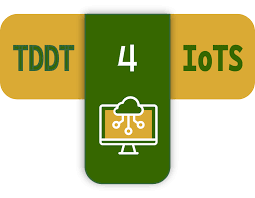
\includegraphics[width=131.75pt,height=102.55pt]{latexImage_9fc631784fec3eb3e8f264ea08b44acd.png}}
\end{picture}
\newpage
\begin{tikzpicture}[overlay]\path(0pt,0pt);\end{tikzpicture}
\begin{picture}(-5,0)(2.5,0)
\put(88.1,-72.97998){\fontsize{14.04}{1}\usefont{T1}{cmr}{b}{n}\selectfont\color{color_29791}14. Análisis de entorno. }
\put(70.104,-94.46002){\fontsize{12}{1}\usefont{T1}{cmr}{m}{n}\selectfont\color{color_29791}El Sistema Inteligente de Monitoreo y Control de Calidad del Aire surge como una }
\put(70.104,-115.22){\fontsize{12}{1}\usefont{T1}{cmr}{m}{n}\selectfont\color{color_29791}solución innovadora y proactiva para abordar la necesidad de proteger la salud de los }
\put(70.104,-135.86){\fontsize{12}{1}\usefont{T1}{cmr}{m}{n}\selectfont\color{color_29791}habitantes del hogar, especialmente de grupos vulnerables como niños, ancianos y }
\put(70.104,-156.62){\fontsize{12}{1}\usefont{T1}{cmr}{m}{n}\selectfont\color{color_29791}personas con condiciones médicas existentes. La calidad del aire en espacios interiores es }
\put(70.104,-177.26){\fontsize{12}{1}\usefont{T1}{cmr}{m}{n}\selectfont\color{color_29791}un aspecto crítico que puede afectar la salud de las personas que habitan en ellos.  }
\put(70.104,-205.94){\fontsize{12}{1}\usefont{T1}{cmr}{m}{n}\selectfont\color{color_29791}Además, el Sistema Inteligente de Monitoreo y Control de Calidad del Aire se enfoca en }
\put(70.104,-226.7){\fontsize{12}{1}\usefont{T1}{cmr}{m}{n}\selectfont\color{color_29791}ofrecer una solución práctica y posible para todos los usuarios, independientemente de }
\put(70.104,-247.34){\fontsize{12}{1}\usefont{T1}{cmr}{m}{n}\selectfont\color{color_29791}sus conocimientos técnicos. La conectividad a internet es fundamental para enviar alertas }
\put(70.104,-268.13){\fontsize{12}{1}\usefont{T1}{cmr}{m}{n}\selectfont\color{color_29791}y notificaciones a los usuarios a través de una aplicación móvil, indicando la naturaleza }
\put(70.104,-288.77){\fontsize{12}{1}\usefont{T1}{cmr}{m}{n}\selectfont\color{color_29791}del problema y las medidas recomendadas para solucionarlo. Se busca que el sistema sea }
\put(70.104,-309.53){\fontsize{12}{1}\usefont{T1}{cmr}{m}{n}\selectfont\color{color_29791}fácil de instalar en cualquier hogar, para ofrecer una solución práctica y mejorar la calidad }
\put(70.104,-330.17){\fontsize{12}{1}\usefont{T1}{cmr}{m}{n}\selectfont\color{color_29791}de vida en casa. Es importante garantizar que el sistema cumpla con los estándares y }
\put(70.104,-350.93){\fontsize{12}{1}\usefont{T1}{cmr}{m}{n}\selectfont\color{color_29791}regulaciones de calidad del aire y seguridad del hogar, para asegurar la protección de la }
\put(70.104,-371.57){\fontsize{12}{1}\usefont{T1}{cmr}{m}{n}\selectfont\color{color_29791}salud de los habitantes del hogar.  }
\put(88.1,-412.13){\fontsize{14.04}{1}\usefont{T1}{cmr}{b}{n}\selectfont\color{color_29791}15. Análisis de viabilidad. }
\put(70.104,-433.63){\fontsize{12}{1}\usefont{T1}{cmr}{m}{n}\selectfont\color{color_29791}Es importante realizar un análisis de viabilidad para detectar las posibilidades y riesgos }
\put(70.104,-454.39){\fontsize{12}{1}\usefont{T1}{cmr}{m}{n}\selectfont\color{color_29791}asociados con la implementación de un proyecto IoT. Los estados de factibilidad de este }
\put(70.104,-475.03){\fontsize{12}{1}\usefont{T1}{cmr}{m}{n}\selectfont\color{color_29791}trabajo son los siguientes: }
\put(88.1,-504.79){\fontsize{12}{1}\usefont{T1}{cmr}{m}{n}\selectfont\color{color_29791}• Viabilidad legal: Es importante cumplir con las regulaciones y estándares de }
\put(106.1,-525.31){\fontsize{12}{1}\usefont{T1}{cmr}{m}{n}\selectfont\color{color_29791}calidad del aire y seguridad del hogar para garantizar la protección de la salud de }
\put(106.1,-546.07){\fontsize{12}{1}\usefont{T1}{cmr}{m}{n}\selectfont\color{color_29791}los habitantes del hogar. Es necesario investigar y cumplir con las leyes y }
\put(106.1,-566.71){\fontsize{12}{1}\usefont{T1}{cmr}{m}{n}\selectfont\color{color_29791}regulaciones locales y nacionales relacionadas con la calidad del aire en espacios }
\put(106.1,-587.47){\fontsize{12}{1}\usefont{T1}{cmr}{m}{n}\selectfont\color{color_29791}interiores. }
\put(88.1,-609.1){\fontsize{12}{1}\usefont{T1}{cmr}{m}{n}\selectfont\color{color_29791}• Viabilidad social: El Sistema Inteligente de Monitoreo y Control de Calidad del }
\put(106.1,-629.74){\fontsize{12}{1}\usefont{T1}{cmr}{m}{n}\selectfont\color{color_29791}Aire tiene un impacto social positivo al mejorar la calidad de vida de los habitantes }
\put(106.1,-650.38){\fontsize{12}{1}\usefont{T1}{cmr}{m}{n}\selectfont\color{color_29791}del hogar, especialmente de grupos vulnerables como niños, ancianos y personas }
\put(106.1,-671.14){\fontsize{12}{1}\usefont{T1}{cmr}{m}{n}\selectfont\color{color_29791}con condiciones médicas existentes. Además, al ser una solución práctica y }
\put(106.1,-691.78){\fontsize{12}{1}\usefont{T1}{cmr}{m}{n}\selectfont\color{color_29791}asequible, puede ser accesible para una amplia gama de usuarios. }
\put(88.1,-713.5){\fontsize{12}{1}\usefont{T1}{cmr}{m}{n}\selectfont\color{color_29791}• Importancia de la calidad del aire en espacios interiores: La contaminación del }
\put(106.1,-734.016){\fontsize{12}{1}\usefont{T1}{cmr}{m}{n}\selectfont\color{color_29791}aire en ambientes cerrados representa un desafío significativo, especialmente en }
\put(106.1,-754.776){\fontsize{12}{1}\usefont{T1}{cmr}{m}{n}\selectfont\color{color_29791}lo que respecta a la detección y control de contaminantes que pueden afectar la }
\end{picture}
\newpage
\begin{tikzpicture}[overlay]\path(0pt,0pt);\end{tikzpicture}
\begin{picture}(-5,0)(2.5,0)
\put(106.1,-71.03998){\fontsize{12}{1}\usefont{T1}{cmr}{m}{n}\selectfont\color{color_29791}salud de quienes habitan allí, en particular, de grupos vulnerables. Por lo tanto, un }
\put(106.1,-91.82001){\fontsize{12}{1}\usefont{T1}{cmr}{m}{n}\selectfont\color{color_29791}sistema de monitoreo y control de calidad del aire en el hogar es crucial para }
\put(106.1,-112.46){\fontsize{12}{1}\usefont{T1}{cmr}{m}{n}\selectfont\color{color_29791}proteger la salud de los residentes. }
\put(70.104,-141.26){\fontsize{12}{1}\usefont{T1}{cmr}{m}{n}\selectfont\color{color_29791} }
\put(88.1,-170.9){\fontsize{12}{1}\usefont{T1}{cmr}{m}{n}\selectfont\color{color_29791}• Necesidad de proteger a grupos vulnerables: Los niños, ancianos y personas con }
\put(106.1,-191.42){\fontsize{12}{1}\usefont{T1}{cmr}{m}{n}\selectfont\color{color_29791}condiciones médicas previas son especialmente susceptibles a los efectos }
\put(106.1,-212.18){\fontsize{12}{1}\usefont{T1}{cmr}{m}{n}\selectfont\color{color_29791}negativos de la mala calidad del aire en espacios interiores. Por lo tanto, contar }
\put(106.1,-232.82){\fontsize{12}{1}\usefont{T1}{cmr}{m}{n}\selectfont\color{color_29791}con un sistema que les brinde protección y alertas ante niveles elevados de }
\put(106.1,-253.61){\fontsize{12}{1}\usefont{T1}{cmr}{m}{n}\selectfont\color{color_29791}contaminación es esencial para su bienestar, }
\put(88.1,-294.17){\fontsize{14.04}{1}\usefont{T1}{cmr}{b}{n}\selectfont\color{color_29791}16. Diseño de la capa tecnológica }
\put(70.104,-315.65){\fontsize{12}{1}\usefont{T1}{cmr}{m}{n}\selectfont\color{color_29791}Durante esta etapa, todos los miembros del equipo del proyecto estuvieron involucrados }
\put(70.104,-336.41){\fontsize{12}{1}\usefont{T1}{cmr}{m}{n}\selectfont\color{color_29791}en la tarea de Diseño de la capa de tecnológica, creando así el primer diseño del sistema }
\put(70.104,-357.05){\fontsize{12}{1}\usefont{T1}{cmr}{m}{n}\selectfont\color{color_29791}global que orientará al equipo de desarrollo. Para llevar a cabo el diseño del sistema, }
\put(70.104,-377.81){\fontsize{12}{1}\usefont{T1}{cmr}{m}{n}\selectfont\color{color_29791}resultó útil emplear la herramienta de diseño de circuitos TDDT4IoTS que permitió }
\put(70.104,-398.45){\fontsize{12}{1}\usefont{T1}{cmr}{m}{n}\selectfont\color{color_29791}representar de manera clara los componentes definidos para el proyecto. Después de }
\put(70.104,-419.09){\fontsize{12}{1}\usefont{T1}{cmr}{m}{n}\selectfont\color{color_29791}obtener el diseño, se pudo analizar los costos de los componentes de hardware que lo }
\put(70.104,-439.87){\fontsize{12}{1}\usefont{T1}{cmr}{m}{n}\selectfont\color{color_29791}integrarán. }
\put(70.104,-468.55){\fontsize{12}{1}\usefont{T1}{cmr}{m}{n}\selectfont\color{color_29791}Los resultados de este trabajo de diseño produjeron el diseño de la arquitectura del IoT, }
\put(70.104,-489.31){\fontsize{12}{1}\usefont{T1}{cmr}{m}{n}\selectfont\color{color_29791}que consta de dos tipos de arquitectura: una de ellas es conocida como la arquitectura de }
\put(70.104,-509.95){\fontsize{12}{1}\usefont{T1}{cmr}{m}{n}\selectfont\color{color_29791}cinco capas, la cual incluye la capa de percepción, capa de transporte, capa de }
\put(70.104,-530.71){\fontsize{12}{1}\usefont{T1}{cmr}{m}{n}\selectfont\color{color_29791}proc}
\put(79.19999,-760.1198){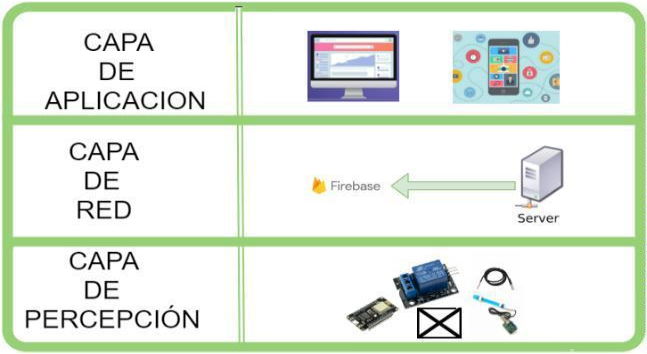
\includegraphics[width=401.9678pt,height=219.334pt]{latexImage_50d62af52a4f31bc9300aea2528508be.png}}
\put(271.12,-746.493){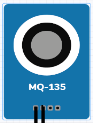
\includegraphics[width=33.614pt,height=44.556pt]{latexImage_882588c6b3903172be82c1a53aff9d6b.png}}
\put(304.73,-745.892){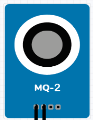
\includegraphics[width=33.614pt,height=43.353pt]{latexImage_fb82b9f8bca3adefade15e4c58accfa6.png}}
\put(338.34,-753.073){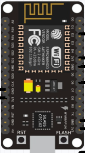
\includegraphics[width=30.928pt,height=55.201pt]{latexImage_51662cfb78b906b9688ee035575b39b5.png}}
\put(370.58,-732.07){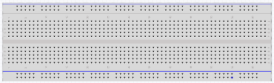
\includegraphics[width=98.938pt,height=30.132pt]{latexImage_c76f7614c7e24111ecfa27694771242d.png}}
\put(414.82,-746.937){
\includegraphics[width=40.43303pt,height=14.86806pt]{latexImage_f1df0345069f0e1e6cf6214aa39dd3ec.png}}
\end{picture}
\newpage
\begin{tikzpicture}[overlay]\path(0pt,0pt);\end{tikzpicture}
\begin{picture}(-5,0)(2.5,0)
\put(70.104,-71.03998){\fontsize{12}{1}\usefont{T1}{cmr}{m}{n}\selectfont\color{color_29791}requerimientos del sistema distribuido para el Sistema Inteligente de Monitoreo y Control }
\put(70.104,-91.82001){\fontsize{12}{1}\usefont{T1}{cmr}{m}{n}\selectfont\color{color_29791}de Calidad del Aire, se han considerado solamente tres capas que son: capa de aplicación, }
\put(70.104,-112.46){\fontsize{12}{1}\usefont{T1}{cmr}{m}{n}\selectfont\color{color_29791}capa de internet y capa de percepción, en la Figura a continuación se ilustra con más }
\put(70.104,-133.22){\fontsize{12}{1}\usefont{T1}{cmr}{m}{n}\selectfont\color{color_29791}detalle los elementos presentes en cada una de estas capas. La capa inferior se denomina }
\put(70.104,-153.86){\fontsize{12}{1}\usefont{T1}{cmr}{m}{n}\selectfont\color{color_29791}capa de percepción, ya que es aquí donde se encuentran los sensores y donde se lleva a }
\put(70.104,-174.62){\fontsize{12}{1}\usefont{T1}{cmr}{m}{n}\selectfont\color{color_29791}cabo el preprocesamiento de la información detectada por los sensores. Esta capa es }
\put(70.104,-195.26){\fontsize{12}{1}\usefont{T1}{cmr}{m}{n}\selectfont\color{color_29791}responsable de realizar las funciones de seguimiento y control del entorno. La capa }
\put(70.104,-216.02){\fontsize{12}{1}\usefont{T1}{cmr}{m}{n}\selectfont\color{color_29791}intermedia, denominada capa de internet, es donde se lleva a cabo tanto la conectividad }
\put(70.104,-236.66){\fontsize{12}{1}\usefont{T1}{cmr}{m}{n}\selectfont\color{color_29791}como el procesamiento y almacenamiento de la información. En esta capa se ubica el  }
\put(215.45,-262.73){\fontsize{9}{1}\usefont{T1}{cmr}{m}{it}\selectfont\color{color_97849}Ilustración 1Arquitectura del sistema }
\put(70.104,-290.93){\fontsize{12}{1}\usefont{T1}{cmr}{m}{n}\selectfont\color{color_29791}servicio Hosting, el cual se utiliza para enviar datos en tiempo real para ser almacenados }
\put(70.104,-311.69){\fontsize{12}{1}\usefont{T1}{cmr}{m}{n}\selectfont\color{color_29791}en la base de datos Firebase [18] y visualizados en ambas aplicaciones (web y móvil). La }
\put(70.104,-332.33){\fontsize{12}{1}\usefont{T1}{cmr}{m}{n}\selectfont\color{color_29791}capa de Aplicación es la capa que permite la interacción del usuario, la cual se compone }
\put(70.104,-353.09){\fontsize{12}{1}\usefont{T1}{cmr}{m}{n}\selectfont\color{color_29791}de dos aplicaciones (web y móvil) a través de las cuales los usuarios pueden interactuar }
\put(70.104,-373.73){\fontsize{12}{1}\usefont{T1}{cmr}{m}{n}\selectfont\color{color_29791}con el sistema. }
\put(70.104,-402.41){\fontsize{12}{1}\usefont{T1}{cmr}{m}{n}\selectfont\color{color_29791}En la Fig. 1 se muestra la arquitectura del sistema IoT esta arquitectura permitirá que los }
\put(70.104,-423.17){\fontsize{12}{1}\usefont{T1}{cmr}{m}{n}\selectfont\color{color_29791}datos capturados por la capa de percepción sean enviados mediante internet al }
\put(70.104,-443.83){\fontsize{12}{1}\usefont{T1}{cmr}{m}{n}\selectfont\color{color_29791}almacenamiento en la nube desde el cual las aplicaciones tanto web y móvil servirán para }
\put(70.104,-464.59){\fontsize{12}{1}\usefont{T1}{cmr}{m}{n}\selectfont\color{color_29791}ingresar datos de configuración para la capa de actuadores, además la aplicación móvil }
\put(70.104,-485.23){\fontsize{12}{1}\usefont{T1}{cmr}{m}{n}\selectfont\color{color_29791}podrá enviar órdenes a los actuadores de la capa de percepción por medio de la capa de }
\put(70.104,-505.99){\fontsize{12}{1}\usefont{T1}{cmr}{m}{n}\selectfont\color{color_29791}internet. }
\end{picture}
\newpage
\begin{tikzpicture}[overlay]\path(0pt,0pt);\end{tikzpicture}
\begin{picture}(-5,0)(2.5,0)
\put(70.104,-71.03998){\fontsize{12}{1}\usefont{T1}{cmr}{m}{n}\selectfont\color{color_29791}El diseño del dispositivo IoT (ilustracion2) permitirá detectar varios datos como }
\put(70.104,-91.82001){\fontsize{12}{1}\usefont{T1}{cmr}{m}{n}\selectfont\color{color_29791}humedad, temperatura, calidad de aire, gas Lp, i-butano, propano, metano, alcohol, }
\put(70.104,-112.46){\fontsize{12}{1}\usefont{T1}{cmr}{m}{n}\selectfont\color{color_29791}hidrógeno. Este esquema se ha desarrollado utilizando la herramienta TDDT4IoTS. Los }
\put(70.104,-133.22){\fontsize{12}{1}\usefont{T1}{cmr}{m}{n}\selectfont\color{color_29791}componentes utilizados son: (A) Sensor MQ2, (B) Sensor MQ 135, (C)DTH11 Sensor de }
\put(70.104,-153.86){\fontsize{12}{1}\usefont{T1}{cmr}{m}{n}\selectfont\color{color_29791}temperatura y humedad, (D) ESP8266 Modulo wifi, (E) Servomotor, (F) Ventilador }
\put(70.104,-458.59){\fontsize{12}{1}\usefont{T1}{cmr}{m}{n}\selectfont\color{color_29791}Las etapas de Análisis preliminar y Diseño de la capa tecnológica no volverán a realizarse }
\put(70.104,-479.35){\fontsize{12}{1}\usefont{T1}{cmr}{m}{n}\selectfont\color{color_29791}debido a que los requisitos de este sistema fueron claros y concretos desde las primeras }
\put(70.104,-499.99){\fontsize{12}{1}\usefont{T1}{cmr}{m}{n}\selectfont\color{color_29791}etapas. Además, la participación de los usuarios en esta etapa fue fundamental para }
\put(70.104,-520.75){\fontsize{12}{1}\usefont{T1}{cmr}{m}{n}\selectfont\color{color_29791}garantizar que el diseño del sistema satisficiera sus necesidades.  }
\put(88.1,-551.35){\fontsize{14.04}{1}\usefont{T1}{cmr}{b}{n}\selectfont\color{color_29791}17. Análisis de costos del dispositivo }
\put(70.104,-574.75){\fontsize{12}{1}\usefont{T1}{cmr}{m}{n}\selectfont\color{color_29791}Es importante conocer el valor de cada uno de los componentes utilizados para calcular }
\put(70.104,-595.51){\fontsize{12}{1}\usefont{T1}{cmr}{m}{n}\selectfont\color{color_29791}con precisión el costo total de construir un dispositivo similar al que se describe aquí. }
\put(70.104,-616.18){\fontsize{12}{1}\usefont{T1}{cmr}{m}{n}\selectfont\color{color_29791}Debido a esto se ha proporcionado una descripción detallada  de cada uno de ellos, para }
\put(70.104,-636.94){\fontsize{12}{1}\usefont{T1}{cmr}{m}{n}\selectfont\color{color_29791}que el lector pueda tener una idea clara de los precios a considerar en su mercado local. }
\put(226.85,-662.98){\fontsize{9}{1}\usefont{T1}{cmr}{m}{it}\selectfont\color{color_97849}Tabla 4 Costos del dispositivos }
\put(132.5,-686.5){\fontsize{12}{1}\usefont{T1}{cmr}{m}{n}\selectfont\color{color_29791}Dispositivo Cantidad Precio }
\end{picture}
\begin{tikzpicture}[overlay]
\path(0pt,0pt);
\filldraw[color_29791][even odd rule]
(126.74pt, -675.34pt) -- (127.22pt, -675.34pt)
 -- (127.22pt, -675.34pt)
 -- (127.22pt, -674.86pt)
 -- (127.22pt, -674.86pt)
 -- (126.74pt, -674.86pt) -- cycle
;
\filldraw[color_29791][even odd rule]
(126.74pt, -675.34pt) -- (127.22pt, -675.34pt)
 -- (127.22pt, -675.34pt)
 -- (127.22pt, -674.86pt)
 -- (127.22pt, -674.86pt)
 -- (126.74pt, -674.86pt) -- cycle
;
\filldraw[color_29791][even odd rule]
(127.22pt, -675.34pt) -- (340.15pt, -675.34pt)
 -- (340.15pt, -675.34pt)
 -- (340.15pt, -674.86pt)
 -- (340.15pt, -674.86pt)
 -- (127.22pt, -674.86pt) -- cycle
;
\filldraw[color_29791][even odd rule]
(340.15pt, -675.34pt) -- (340.63pt, -675.34pt)
 -- (340.63pt, -675.34pt)
 -- (340.63pt, -674.86pt)
 -- (340.63pt, -674.86pt)
 -- (340.15pt, -674.86pt) -- cycle
;
\filldraw[color_29791][even odd rule]
(340.63pt, -675.34pt) -- (394.27pt, -675.34pt)
 -- (394.27pt, -675.34pt)
 -- (394.27pt, -674.86pt)
 -- (394.27pt, -674.86pt)
 -- (340.63pt, -674.86pt) -- cycle
;
\filldraw[color_29791][even odd rule]
(394.27pt, -675.34pt) -- (394.75pt, -675.34pt)
 -- (394.75pt, -675.34pt)
 -- (394.75pt, -674.86pt)
 -- (394.75pt, -674.86pt)
 -- (394.27pt, -674.86pt) -- cycle
;
\filldraw[color_29791][even odd rule]
(394.75pt, -675.34pt) -- (438.094pt, -675.34pt)
 -- (438.094pt, -675.34pt)
 -- (438.094pt, -674.86pt)
 -- (438.094pt, -674.86pt)
 -- (394.75pt, -674.86pt) -- cycle
;
\filldraw[color_29791][even odd rule]
(438.1pt, -675.34pt) -- (438.58pt, -675.34pt)
 -- (438.58pt, -675.34pt)
 -- (438.58pt, -674.86pt)
 -- (438.58pt, -674.86pt)
 -- (438.1pt, -674.86pt) -- cycle
;
\filldraw[color_29791][even odd rule]
(438.1pt, -675.34pt) -- (438.58pt, -675.34pt)
 -- (438.58pt, -675.34pt)
 -- (438.58pt, -674.86pt)
 -- (438.58pt, -674.86pt)
 -- (438.1pt, -674.86pt) -- cycle
;
\filldraw[color_29791][even odd rule]
(126.74pt, -695.98pt) -- (127.22pt, -695.98pt)
 -- (127.22pt, -695.98pt)
 -- (127.22pt, -675.34pt)
 -- (127.22pt, -675.34pt)
 -- (126.74pt, -675.34pt) -- cycle
;
\filldraw[color_29791][even odd rule]
(340.15pt, -695.98pt) -- (340.63pt, -695.98pt)
 -- (340.63pt, -695.98pt)
 -- (340.63pt, -675.34pt)
 -- (340.63pt, -675.34pt)
 -- (340.15pt, -675.34pt) -- cycle
;
\filldraw[color_29791][even odd rule]
(394.27pt, -695.98pt) -- (394.75pt, -695.98pt)
 -- (394.75pt, -695.98pt)
 -- (394.75pt, -675.34pt)
 -- (394.75pt, -675.34pt)
 -- (394.27pt, -675.34pt) -- cycle
;
\filldraw[color_29791][even odd rule]
(438.1pt, -695.98pt) -- (438.58pt, -695.98pt)
 -- (438.58pt, -695.98pt)
 -- (438.58pt, -675.34pt)
 -- (438.58pt, -675.34pt)
 -- (438.1pt, -675.34pt) -- cycle
;
\begin{scope}
\clip
(127.34pt, -717.22pt) -- (340.15pt, -717.22pt)
 -- (340.15pt, -717.22pt)
 -- (340.15pt, -696.46pt)
 -- (340.15pt, -696.46pt)
 -- (127.34pt, -696.46pt) -- cycle
;
\begin{scope}
\clip
(127.34pt, -717.22pt) -- (340.15pt, -717.22pt)
 -- (340.15pt, -717.22pt)
 -- (340.15pt, -696.46pt)
 -- (340.15pt, -696.46pt)
 -- (127.34pt, -696.46pt) -- cycle
;
\end{scope}
\end{scope}
\end{tikzpicture}
\begin{picture}(-5,0)(2.5,0)
\put(132.5,-707.62){\fontsize{12}{1}\usefont{T1}{cmr}{m}{n}\selectfont\color{color_29791}Protoboard 830 puntos 1 \$4.49 }
\end{picture}
\begin{tikzpicture}[overlay]
\path(0pt,0pt);
\filldraw[color_29791][even odd rule]
(126.74pt, -696.46pt) -- (127.22pt, -696.46pt)
 -- (127.22pt, -696.46pt)
 -- (127.22pt, -695.98pt)
 -- (127.22pt, -695.98pt)
 -- (126.74pt, -695.98pt) -- cycle
;
\filldraw[color_29791][even odd rule]
(127.22pt, -696.46pt) -- (340.15pt, -696.46pt)
 -- (340.15pt, -696.46pt)
 -- (340.15pt, -695.98pt)
 -- (340.15pt, -695.98pt)
 -- (127.22pt, -695.98pt) -- cycle
;
\filldraw[color_29791][even odd rule]
(340.15pt, -696.46pt) -- (340.63pt, -696.46pt)
 -- (340.63pt, -696.46pt)
 -- (340.63pt, -695.98pt)
 -- (340.63pt, -695.98pt)
 -- (340.15pt, -695.98pt) -- cycle
;
\filldraw[color_29791][even odd rule]
(340.63pt, -696.46pt) -- (394.27pt, -696.46pt)
 -- (394.27pt, -696.46pt)
 -- (394.27pt, -695.98pt)
 -- (394.27pt, -695.98pt)
 -- (340.63pt, -695.98pt) -- cycle
;
\filldraw[color_29791][even odd rule]
(394.27pt, -696.46pt) -- (394.75pt, -696.46pt)
 -- (394.75pt, -696.46pt)
 -- (394.75pt, -695.98pt)
 -- (394.75pt, -695.98pt)
 -- (394.27pt, -695.98pt) -- cycle
;
\filldraw[color_29791][even odd rule]
(394.75pt, -696.46pt) -- (438.094pt, -696.46pt)
 -- (438.094pt, -696.46pt)
 -- (438.094pt, -695.98pt)
 -- (438.094pt, -695.98pt)
 -- (394.75pt, -695.98pt) -- cycle
;
\filldraw[color_29791][even odd rule]
(438.1pt, -696.46pt) -- (438.58pt, -696.46pt)
 -- (438.58pt, -696.46pt)
 -- (438.58pt, -695.98pt)
 -- (438.58pt, -695.98pt)
 -- (438.1pt, -695.98pt) -- cycle
;
\filldraw[color_29791][even odd rule]
(126.74pt, -717.22pt) -- (127.22pt, -717.22pt)
 -- (127.22pt, -717.22pt)
 -- (127.22pt, -696.46pt)
 -- (127.22pt, -696.46pt)
 -- (126.74pt, -696.46pt) -- cycle
;
\filldraw[color_29791][even odd rule]
(340.15pt, -717.22pt) -- (340.63pt, -717.22pt)
 -- (340.63pt, -717.22pt)
 -- (340.63pt, -696.46pt)
 -- (340.63pt, -696.46pt)
 -- (340.15pt, -696.46pt) -- cycle
;
\filldraw[color_29791][even odd rule]
(394.27pt, -717.22pt) -- (394.75pt, -717.22pt)
 -- (394.75pt, -717.22pt)
 -- (394.75pt, -696.46pt)
 -- (394.75pt, -696.46pt)
 -- (394.27pt, -696.46pt) -- cycle
;
\filldraw[color_29791][even odd rule]
(438.1pt, -717.22pt) -- (438.58pt, -717.22pt)
 -- (438.58pt, -717.22pt)
 -- (438.58pt, -696.46pt)
 -- (438.58pt, -696.46pt)
 -- (438.1pt, -696.46pt) -- cycle
;
\begin{scope}
\clip
(127.34pt, -738.456pt) -- (340.15pt, -738.456pt)
 -- (340.15pt, -738.456pt)
 -- (340.15pt, -717.696pt)
 -- (340.15pt, -717.696pt)
 -- (127.34pt, -717.696pt) -- cycle
;
\begin{scope}
\clip
(127.34pt, -738.456pt) -- (340.15pt, -738.456pt)
 -- (340.15pt, -738.456pt)
 -- (340.15pt, -717.696pt)
 -- (340.15pt, -717.696pt)
 -- (127.34pt, -717.696pt) -- cycle
;
\end{scope}
\end{scope}
\end{tikzpicture}
\begin{picture}(-5,0)(2.5,0)
\put(132.5,-728.86){\fontsize{12}{1}\usefont{T1}{cmr}{m}{n}\selectfont\color{color_29791}Sensor MQ2 1 \$3.99 }
\end{picture}
\begin{tikzpicture}[overlay]
\path(0pt,0pt);
\filldraw[color_29791][even odd rule]
(126.74pt, -717.7pt) -- (127.22pt, -717.7pt)
 -- (127.22pt, -717.7pt)
 -- (127.22pt, -717.22pt)
 -- (127.22pt, -717.22pt)
 -- (126.74pt, -717.22pt) -- cycle
;
\filldraw[color_29791][even odd rule]
(127.22pt, -717.7pt) -- (340.15pt, -717.7pt)
 -- (340.15pt, -717.7pt)
 -- (340.15pt, -717.22pt)
 -- (340.15pt, -717.22pt)
 -- (127.22pt, -717.22pt) -- cycle
;
\filldraw[color_29791][even odd rule]
(340.15pt, -717.7pt) -- (340.63pt, -717.7pt)
 -- (340.63pt, -717.7pt)
 -- (340.63pt, -717.22pt)
 -- (340.63pt, -717.22pt)
 -- (340.15pt, -717.22pt) -- cycle
;
\filldraw[color_29791][even odd rule]
(340.63pt, -717.7pt) -- (394.27pt, -717.7pt)
 -- (394.27pt, -717.7pt)
 -- (394.27pt, -717.22pt)
 -- (394.27pt, -717.22pt)
 -- (340.63pt, -717.22pt) -- cycle
;
\filldraw[color_29791][even odd rule]
(394.27pt, -717.7pt) -- (394.75pt, -717.7pt)
 -- (394.75pt, -717.7pt)
 -- (394.75pt, -717.22pt)
 -- (394.75pt, -717.22pt)
 -- (394.27pt, -717.22pt) -- cycle
;
\filldraw[color_29791][even odd rule]
(394.75pt, -717.7pt) -- (438.094pt, -717.7pt)
 -- (438.094pt, -717.7pt)
 -- (438.094pt, -717.22pt)
 -- (438.094pt, -717.22pt)
 -- (394.75pt, -717.22pt) -- cycle
;
\filldraw[color_29791][even odd rule]
(438.1pt, -717.7pt) -- (438.58pt, -717.7pt)
 -- (438.58pt, -717.7pt)
 -- (438.58pt, -717.22pt)
 -- (438.58pt, -717.22pt)
 -- (438.1pt, -717.22pt) -- cycle
;
\filldraw[color_29791][even odd rule]
(126.74pt, -738.456pt) -- (127.22pt, -738.456pt)
 -- (127.22pt, -738.456pt)
 -- (127.22pt, -717.696pt)
 -- (127.22pt, -717.696pt)
 -- (126.74pt, -717.696pt) -- cycle
;
\filldraw[color_29791][even odd rule]
(340.15pt, -738.456pt) -- (340.63pt, -738.456pt)
 -- (340.63pt, -738.456pt)
 -- (340.63pt, -717.696pt)
 -- (340.63pt, -717.696pt)
 -- (340.15pt, -717.696pt) -- cycle
;
\filldraw[color_29791][even odd rule]
(394.27pt, -738.456pt) -- (394.75pt, -738.456pt)
 -- (394.75pt, -738.456pt)
 -- (394.75pt, -717.696pt)
 -- (394.75pt, -717.696pt)
 -- (394.27pt, -717.696pt) -- cycle
;
\filldraw[color_29791][even odd rule]
(438.1pt, -738.456pt) -- (438.58pt, -738.456pt)
 -- (438.58pt, -738.456pt)
 -- (438.58pt, -717.696pt)
 -- (438.58pt, -717.696pt)
 -- (438.1pt, -717.696pt) -- cycle
;
\begin{scope}
\clip
(127.34pt, -759.576pt) -- (340.15pt, -759.576pt)
 -- (340.15pt, -759.576pt)
 -- (340.15pt, -738.936pt)
 -- (340.15pt, -738.936pt)
 -- (127.34pt, -738.936pt) -- cycle
;
\begin{scope}
\clip
(127.34pt, -759.576pt) -- (340.15pt, -759.576pt)
 -- (340.15pt, -759.576pt)
 -- (340.15pt, -738.936pt)
 -- (340.15pt, -738.936pt)
 -- (127.34pt, -738.936pt) -- cycle
;
\end{scope}
\end{scope}
\end{tikzpicture}
\begin{picture}(-5,0)(2.5,0)
\put(132.5,-750.096){\fontsize{12}{1}\usefont{T1}{cmr}{m}{n}\selectfont\color{color_29791}Sensor MQ 135 1 \$3.99 }
\end{picture}
\begin{tikzpicture}[overlay]
\path(0pt,0pt);
\filldraw[color_29791][even odd rule]
(126.74pt, -738.936pt) -- (127.22pt, -738.936pt)
 -- (127.22pt, -738.936pt)
 -- (127.22pt, -738.4559pt)
 -- (127.22pt, -738.4559pt)
 -- (126.74pt, -738.4559pt) -- cycle
;
\filldraw[color_29791][even odd rule]
(127.22pt, -738.936pt) -- (340.15pt, -738.936pt)
 -- (340.15pt, -738.936pt)
 -- (340.15pt, -738.4559pt)
 -- (340.15pt, -738.4559pt)
 -- (127.22pt, -738.4559pt) -- cycle
;
\filldraw[color_29791][even odd rule]
(340.15pt, -738.936pt) -- (340.63pt, -738.936pt)
 -- (340.63pt, -738.936pt)
 -- (340.63pt, -738.4559pt)
 -- (340.63pt, -738.4559pt)
 -- (340.15pt, -738.4559pt) -- cycle
;
\filldraw[color_29791][even odd rule]
(340.63pt, -738.936pt) -- (394.27pt, -738.936pt)
 -- (394.27pt, -738.936pt)
 -- (394.27pt, -738.4559pt)
 -- (394.27pt, -738.4559pt)
 -- (340.63pt, -738.4559pt) -- cycle
;
\filldraw[color_29791][even odd rule]
(394.27pt, -738.936pt) -- (394.75pt, -738.936pt)
 -- (394.75pt, -738.936pt)
 -- (394.75pt, -738.4559pt)
 -- (394.75pt, -738.4559pt)
 -- (394.27pt, -738.4559pt) -- cycle
;
\filldraw[color_29791][even odd rule]
(394.75pt, -738.936pt) -- (438.094pt, -738.936pt)
 -- (438.094pt, -738.936pt)
 -- (438.094pt, -738.4559pt)
 -- (438.094pt, -738.4559pt)
 -- (394.75pt, -738.4559pt) -- cycle
;
\filldraw[color_29791][even odd rule]
(438.1pt, -738.936pt) -- (438.58pt, -738.936pt)
 -- (438.58pt, -738.936pt)
 -- (438.58pt, -738.4559pt)
 -- (438.58pt, -738.4559pt)
 -- (438.1pt, -738.4559pt) -- cycle
;
\filldraw[color_29791][even odd rule]
(126.74pt, -759.576pt) -- (127.22pt, -759.576pt)
 -- (127.22pt, -759.576pt)
 -- (127.22pt, -738.936pt)
 -- (127.22pt, -738.936pt)
 -- (126.74pt, -738.936pt) -- cycle
;
\filldraw[color_29791][even odd rule]
(126.74pt, -760.056pt) -- (127.22pt, -760.056pt)
 -- (127.22pt, -760.056pt)
 -- (127.22pt, -759.576pt)
 -- (127.22pt, -759.576pt)
 -- (126.74pt, -759.576pt) -- cycle
;
\filldraw[color_29791][even odd rule]
(126.74pt, -760.056pt) -- (127.22pt, -760.056pt)
 -- (127.22pt, -760.056pt)
 -- (127.22pt, -759.576pt)
 -- (127.22pt, -759.576pt)
 -- (126.74pt, -759.576pt) -- cycle
;
\filldraw[color_29791][even odd rule]
(127.22pt, -760.056pt) -- (340.15pt, -760.056pt)
 -- (340.15pt, -760.056pt)
 -- (340.15pt, -759.576pt)
 -- (340.15pt, -759.576pt)
 -- (127.22pt, -759.576pt) -- cycle
;
\filldraw[color_29791][even odd rule]
(340.15pt, -759.576pt) -- (340.63pt, -759.576pt)
 -- (340.63pt, -759.576pt)
 -- (340.63pt, -738.936pt)
 -- (340.63pt, -738.936pt)
 -- (340.15pt, -738.936pt) -- cycle
;
\filldraw[color_29791][even odd rule]
(340.15pt, -760.056pt) -- (340.63pt, -760.056pt)
 -- (340.63pt, -760.056pt)
 -- (340.63pt, -759.576pt)
 -- (340.63pt, -759.576pt)
 -- (340.15pt, -759.576pt) -- cycle
;
\filldraw[color_29791][even odd rule]
(340.63pt, -760.056pt) -- (394.27pt, -760.056pt)
 -- (394.27pt, -760.056pt)
 -- (394.27pt, -759.576pt)
 -- (394.27pt, -759.576pt)
 -- (340.63pt, -759.576pt) -- cycle
;
\filldraw[color_29791][even odd rule]
(394.27pt, -759.576pt) -- (394.75pt, -759.576pt)
 -- (394.75pt, -759.576pt)
 -- (394.75pt, -738.936pt)
 -- (394.75pt, -738.936pt)
 -- (394.27pt, -738.936pt) -- cycle
;
\filldraw[color_29791][even odd rule]
(394.27pt, -760.056pt) -- (394.75pt, -760.056pt)
 -- (394.75pt, -760.056pt)
 -- (394.75pt, -759.576pt)
 -- (394.75pt, -759.576pt)
 -- (394.27pt, -759.576pt) -- cycle
;
\filldraw[color_29791][even odd rule]
(394.75pt, -760.056pt) -- (438.094pt, -760.056pt)
 -- (438.094pt, -760.056pt)
 -- (438.094pt, -759.576pt)
 -- (438.094pt, -759.576pt)
 -- (394.75pt, -759.576pt) -- cycle
;
\filldraw[color_29791][even odd rule]
(438.1pt, -759.576pt) -- (438.58pt, -759.576pt)
 -- (438.58pt, -759.576pt)
 -- (438.58pt, -738.936pt)
 -- (438.58pt, -738.936pt)
 -- (438.1pt, -738.936pt) -- cycle
;
\filldraw[color_29791][even odd rule]
(438.1pt, -760.056pt) -- (438.58pt, -760.056pt)
 -- (438.58pt, -760.056pt)
 -- (438.58pt, -759.576pt)
 -- (438.58pt, -759.576pt)
 -- (438.1pt, -759.576pt) -- cycle
;
\filldraw[color_29791][even odd rule]
(438.1pt, -760.056pt) -- (438.58pt, -760.056pt)
 -- (438.58pt, -760.056pt)
 -- (438.58pt, -759.576pt)
 -- (438.58pt, -759.576pt)
 -- (438.1pt, -759.576pt) -- cycle
;
\begin{scope}
\clip
(69.75pt, -414.13pt) -- (494.95pt, -414.13pt)
 -- (494.95pt, -414.13pt)
 -- (494.95pt, -174.93pt)
 -- (494.95pt, -174.93pt)
 -- (69.75pt, -174.93pt) -- cycle
;
\end{scope}
\end{tikzpicture}
\begin{picture}(-5,0)(2.5,0)
\put(69.75,-414.13){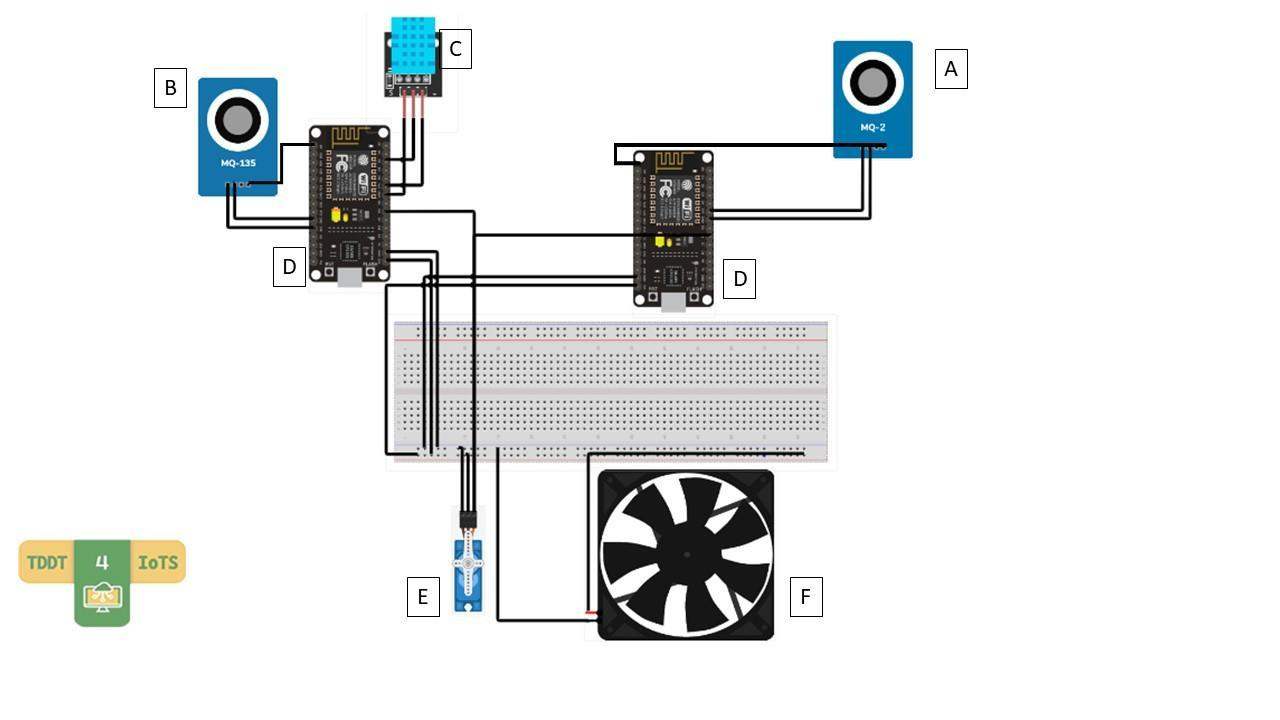
\includegraphics[width=425.2pt,height=239.2pt]{latexImage_42a3a6ebbb9f22dcdbb48a9f9a151f9f.png}}
\end{picture}
\begin{tikzpicture}[overlay]
\path(0pt,0pt);
\filldraw[color_283006][even odd rule]
(69.75pt, -434.73pt) -- (494.95pt, -434.73pt)
 -- (494.95pt, -434.73pt)
 -- (494.95pt, -414.38pt)
 -- (494.95pt, -414.38pt)
 -- (69.75pt, -414.38pt) -- cycle
;
\begin{scope}
\clip
(69.744pt, -434.83pt) -- (495.094pt, -434.83pt)
 -- (495.094pt, -434.83pt)
 -- (495.094pt, -414.406pt)
 -- (495.094pt, -414.406pt)
 -- (69.744pt, -414.406pt) -- cycle
;
\begin{scope}
\clip
(69.744pt, -434.83pt) -- (495.094pt, -434.83pt)
 -- (495.094pt, -434.83pt)
 -- (495.094pt, -414.406pt)
 -- (495.094pt, -414.406pt)
 -- (69.744pt, -414.406pt) -- cycle
;
\end{scope}
\end{scope}
\end{tikzpicture}
\begin{picture}(-5,0)(2.5,0)
\put(210.65,-422.93){\fontsize{9}{1}\usefont{T1}{cmr}{m}{it}\selectfont\color{color_97849}Ilustración 2 Diseño del dispositivo IoT }
\end{picture}
\newpage
\begin{tikzpicture}[overlay]\path(0pt,0pt);\end{tikzpicture}
\begin{picture}(-5,0)(2.5,0)
\put(132.5,-71.64001){\fontsize{12}{1}\usefont{T1}{cmr}{m}{n}\selectfont\color{color_29791}DTH11 Sensor de temperatura y humedad 1 \$6.25 }
\end{picture}
\begin{tikzpicture}[overlay]
\path(0pt,0pt);
\filldraw[color_29791][even odd rule]
(126.74pt, -60.35999pt) -- (127.22pt, -60.35999pt)
 -- (127.22pt, -60.35999pt)
 -- (127.22pt, -59.88pt)
 -- (127.22pt, -59.88pt)
 -- (126.74pt, -59.88pt) -- cycle
;
\filldraw[color_29791][even odd rule]
(126.74pt, -60.35999pt) -- (127.22pt, -60.35999pt)
 -- (127.22pt, -60.35999pt)
 -- (127.22pt, -59.88pt)
 -- (127.22pt, -59.88pt)
 -- (126.74pt, -59.88pt) -- cycle
;
\filldraw[color_29791][even odd rule]
(127.22pt, -60.35999pt) -- (340.15pt, -60.35999pt)
 -- (340.15pt, -60.35999pt)
 -- (340.15pt, -59.88pt)
 -- (340.15pt, -59.88pt)
 -- (127.22pt, -59.88pt) -- cycle
;
\filldraw[color_29791][even odd rule]
(340.15pt, -60.35999pt) -- (340.63pt, -60.35999pt)
 -- (340.63pt, -60.35999pt)
 -- (340.63pt, -59.88pt)
 -- (340.63pt, -59.88pt)
 -- (340.15pt, -59.88pt) -- cycle
;
\filldraw[color_29791][even odd rule]
(340.63pt, -60.35999pt) -- (394.27pt, -60.35999pt)
 -- (394.27pt, -60.35999pt)
 -- (394.27pt, -59.88pt)
 -- (394.27pt, -59.88pt)
 -- (340.63pt, -59.88pt) -- cycle
;
\filldraw[color_29791][even odd rule]
(394.27pt, -60.35999pt) -- (394.75pt, -60.35999pt)
 -- (394.75pt, -60.35999pt)
 -- (394.75pt, -59.88pt)
 -- (394.75pt, -59.88pt)
 -- (394.27pt, -59.88pt) -- cycle
;
\filldraw[color_29791][even odd rule]
(394.75pt, -60.35999pt) -- (438.094pt, -60.35999pt)
 -- (438.094pt, -60.35999pt)
 -- (438.094pt, -59.88pt)
 -- (438.094pt, -59.88pt)
 -- (394.75pt, -59.88pt) -- cycle
;
\filldraw[color_29791][even odd rule]
(438.1pt, -60.35999pt) -- (438.58pt, -60.35999pt)
 -- (438.58pt, -60.35999pt)
 -- (438.58pt, -59.88pt)
 -- (438.58pt, -59.88pt)
 -- (438.1pt, -59.88pt) -- cycle
;
\filldraw[color_29791][even odd rule]
(438.1pt, -60.35999pt) -- (438.58pt, -60.35999pt)
 -- (438.58pt, -60.35999pt)
 -- (438.58pt, -59.88pt)
 -- (438.58pt, -59.88pt)
 -- (438.1pt, -59.88pt) -- cycle
;
\filldraw[color_29791][even odd rule]
(126.74pt, -81.14001pt) -- (127.22pt, -81.14001pt)
 -- (127.22pt, -81.14001pt)
 -- (127.22pt, -60.35602pt)
 -- (127.22pt, -60.35602pt)
 -- (126.74pt, -60.35602pt) -- cycle
;
\filldraw[color_29791][even odd rule]
(340.15pt, -81.14001pt) -- (340.63pt, -81.14001pt)
 -- (340.63pt, -81.14001pt)
 -- (340.63pt, -60.35602pt)
 -- (340.63pt, -60.35602pt)
 -- (340.15pt, -60.35602pt) -- cycle
;
\filldraw[color_29791][even odd rule]
(394.27pt, -81.14001pt) -- (394.75pt, -81.14001pt)
 -- (394.75pt, -81.14001pt)
 -- (394.75pt, -60.35602pt)
 -- (394.75pt, -60.35602pt)
 -- (394.27pt, -60.35602pt) -- cycle
;
\filldraw[color_29791][even odd rule]
(438.1pt, -81.14001pt) -- (438.58pt, -81.14001pt)
 -- (438.58pt, -81.14001pt)
 -- (438.58pt, -60.35602pt)
 -- (438.58pt, -60.35602pt)
 -- (438.1pt, -60.35602pt) -- cycle
;
\begin{scope}
\clip
(127.34pt, -102.38pt) -- (340.15pt, -102.38pt)
 -- (340.15pt, -102.38pt)
 -- (340.15pt, -81.62pt)
 -- (340.15pt, -81.62pt)
 -- (127.34pt, -81.62pt) -- cycle
;
\begin{scope}
\clip
(127.34pt, -102.38pt) -- (340.15pt, -102.38pt)
 -- (340.15pt, -102.38pt)
 -- (340.15pt, -81.62pt)
 -- (340.15pt, -81.62pt)
 -- (127.34pt, -81.62pt) -- cycle
;
\end{scope}
\end{scope}
\end{tikzpicture}
\begin{picture}(-5,0)(2.5,0)
\put(132.5,-92.78003){\fontsize{12}{1}\usefont{T1}{cmr}{m}{n}\selectfont\color{color_29791}ESP8266 Modulo wifi  2 \$8.00 }
\end{picture}
\begin{tikzpicture}[overlay]
\path(0pt,0pt);
\filldraw[color_29791][even odd rule]
(126.74pt, -81.62pt) -- (127.22pt, -81.62pt)
 -- (127.22pt, -81.62pt)
 -- (127.22pt, -81.14001pt)
 -- (127.22pt, -81.14001pt)
 -- (126.74pt, -81.14001pt) -- cycle
;
\filldraw[color_29791][even odd rule]
(127.22pt, -81.62pt) -- (340.15pt, -81.62pt)
 -- (340.15pt, -81.62pt)
 -- (340.15pt, -81.14001pt)
 -- (340.15pt, -81.14001pt)
 -- (127.22pt, -81.14001pt) -- cycle
;
\filldraw[color_29791][even odd rule]
(340.15pt, -81.62pt) -- (340.63pt, -81.62pt)
 -- (340.63pt, -81.62pt)
 -- (340.63pt, -81.14001pt)
 -- (340.63pt, -81.14001pt)
 -- (340.15pt, -81.14001pt) -- cycle
;
\filldraw[color_29791][even odd rule]
(340.63pt, -81.62pt) -- (394.27pt, -81.62pt)
 -- (394.27pt, -81.62pt)
 -- (394.27pt, -81.14001pt)
 -- (394.27pt, -81.14001pt)
 -- (340.63pt, -81.14001pt) -- cycle
;
\filldraw[color_29791][even odd rule]
(394.27pt, -81.62pt) -- (394.75pt, -81.62pt)
 -- (394.75pt, -81.62pt)
 -- (394.75pt, -81.14001pt)
 -- (394.75pt, -81.14001pt)
 -- (394.27pt, -81.14001pt) -- cycle
;
\filldraw[color_29791][even odd rule]
(394.75pt, -81.62pt) -- (438.094pt, -81.62pt)
 -- (438.094pt, -81.62pt)
 -- (438.094pt, -81.14001pt)
 -- (438.094pt, -81.14001pt)
 -- (394.75pt, -81.14001pt) -- cycle
;
\filldraw[color_29791][even odd rule]
(438.1pt, -81.62pt) -- (438.58pt, -81.62pt)
 -- (438.58pt, -81.62pt)
 -- (438.58pt, -81.14001pt)
 -- (438.58pt, -81.14001pt)
 -- (438.1pt, -81.14001pt) -- cycle
;
\filldraw[color_29791][even odd rule]
(126.74pt, -102.38pt) -- (127.22pt, -102.38pt)
 -- (127.22pt, -102.38pt)
 -- (127.22pt, -81.62pt)
 -- (127.22pt, -81.62pt)
 -- (126.74pt, -81.62pt) -- cycle
;
\filldraw[color_29791][even odd rule]
(340.15pt, -102.38pt) -- (340.63pt, -102.38pt)
 -- (340.63pt, -102.38pt)
 -- (340.63pt, -81.62pt)
 -- (340.63pt, -81.62pt)
 -- (340.15pt, -81.62pt) -- cycle
;
\filldraw[color_29791][even odd rule]
(394.27pt, -102.38pt) -- (394.75pt, -102.38pt)
 -- (394.75pt, -102.38pt)
 -- (394.75pt, -81.62pt)
 -- (394.75pt, -81.62pt)
 -- (394.27pt, -81.62pt) -- cycle
;
\filldraw[color_29791][even odd rule]
(438.1pt, -102.38pt) -- (438.58pt, -102.38pt)
 -- (438.58pt, -102.38pt)
 -- (438.58pt, -81.62pt)
 -- (438.58pt, -81.62pt)
 -- (438.1pt, -81.62pt) -- cycle
;
\begin{scope}
\clip
(127.34pt, -123.5pt) -- (340.15pt, -123.5pt)
 -- (340.15pt, -123.5pt)
 -- (340.15pt, -102.86pt)
 -- (340.15pt, -102.86pt)
 -- (127.34pt, -102.86pt) -- cycle
;
\begin{scope}
\clip
(127.34pt, -123.5pt) -- (340.15pt, -123.5pt)
 -- (340.15pt, -123.5pt)
 -- (340.15pt, -102.86pt)
 -- (340.15pt, -102.86pt)
 -- (127.34pt, -102.86pt) -- cycle
;
\end{scope}
\end{scope}
\end{tikzpicture}
\begin{picture}(-5,0)(2.5,0)
\put(132.5,-114.02){\fontsize{12}{1}\usefont{T1}{cmr}{m}{n}\selectfont\color{color_29791}Servomotor 1 \$2.80 }
\end{picture}
\begin{tikzpicture}[overlay]
\path(0pt,0pt);
\filldraw[color_29791][even odd rule]
(126.74pt, -102.86pt) -- (127.22pt, -102.86pt)
 -- (127.22pt, -102.86pt)
 -- (127.22pt, -102.38pt)
 -- (127.22pt, -102.38pt)
 -- (126.74pt, -102.38pt) -- cycle
;
\filldraw[color_29791][even odd rule]
(127.22pt, -102.86pt) -- (340.15pt, -102.86pt)
 -- (340.15pt, -102.86pt)
 -- (340.15pt, -102.38pt)
 -- (340.15pt, -102.38pt)
 -- (127.22pt, -102.38pt) -- cycle
;
\filldraw[color_29791][even odd rule]
(340.15pt, -102.86pt) -- (340.63pt, -102.86pt)
 -- (340.63pt, -102.86pt)
 -- (340.63pt, -102.38pt)
 -- (340.63pt, -102.38pt)
 -- (340.15pt, -102.38pt) -- cycle
;
\filldraw[color_29791][even odd rule]
(340.63pt, -102.86pt) -- (394.27pt, -102.86pt)
 -- (394.27pt, -102.86pt)
 -- (394.27pt, -102.38pt)
 -- (394.27pt, -102.38pt)
 -- (340.63pt, -102.38pt) -- cycle
;
\filldraw[color_29791][even odd rule]
(394.27pt, -102.86pt) -- (394.75pt, -102.86pt)
 -- (394.75pt, -102.86pt)
 -- (394.75pt, -102.38pt)
 -- (394.75pt, -102.38pt)
 -- (394.27pt, -102.38pt) -- cycle
;
\filldraw[color_29791][even odd rule]
(394.75pt, -102.86pt) -- (438.094pt, -102.86pt)
 -- (438.094pt, -102.86pt)
 -- (438.094pt, -102.38pt)
 -- (438.094pt, -102.38pt)
 -- (394.75pt, -102.38pt) -- cycle
;
\filldraw[color_29791][even odd rule]
(438.1pt, -102.86pt) -- (438.58pt, -102.86pt)
 -- (438.58pt, -102.86pt)
 -- (438.58pt, -102.38pt)
 -- (438.58pt, -102.38pt)
 -- (438.1pt, -102.38pt) -- cycle
;
\filldraw[color_29791][even odd rule]
(126.74pt, -123.5pt) -- (127.22pt, -123.5pt)
 -- (127.22pt, -123.5pt)
 -- (127.22pt, -102.86pt)
 -- (127.22pt, -102.86pt)
 -- (126.74pt, -102.86pt) -- cycle
;
\filldraw[color_29791][even odd rule]
(340.15pt, -123.5pt) -- (340.63pt, -123.5pt)
 -- (340.63pt, -123.5pt)
 -- (340.63pt, -102.86pt)
 -- (340.63pt, -102.86pt)
 -- (340.15pt, -102.86pt) -- cycle
;
\filldraw[color_29791][even odd rule]
(394.27pt, -123.5pt) -- (394.75pt, -123.5pt)
 -- (394.75pt, -123.5pt)
 -- (394.75pt, -102.86pt)
 -- (394.75pt, -102.86pt)
 -- (394.27pt, -102.86pt) -- cycle
;
\filldraw[color_29791][even odd rule]
(438.1pt, -123.5pt) -- (438.58pt, -123.5pt)
 -- (438.58pt, -123.5pt)
 -- (438.58pt, -102.86pt)
 -- (438.58pt, -102.86pt)
 -- (438.1pt, -102.86pt) -- cycle
;
\begin{scope}
\clip
(127.34pt, -144.74pt) -- (340.15pt, -144.74pt)
 -- (340.15pt, -144.74pt)
 -- (340.15pt, -124.1pt)
 -- (340.15pt, -124.1pt)
 -- (127.34pt, -124.1pt) -- cycle
;
\begin{scope}
\clip
(127.34pt, -144.74pt) -- (340.15pt, -144.74pt)
 -- (340.15pt, -144.74pt)
 -- (340.15pt, -124.1pt)
 -- (340.15pt, -124.1pt)
 -- (127.34pt, -124.1pt) -- cycle
;
\end{scope}
\end{scope}
\end{tikzpicture}
\begin{picture}(-5,0)(2.5,0)
\put(132.5,-135.26){\fontsize{12}{1}\usefont{T1}{cmr}{m}{n}\selectfont\color{color_29791}Ventilador 1 \$2.67 }
\end{picture}
\begin{tikzpicture}[overlay]
\path(0pt,0pt);
\filldraw[color_29791][even odd rule]
(126.74pt, -123.98pt) -- (127.22pt, -123.98pt)
 -- (127.22pt, -123.98pt)
 -- (127.22pt, -123.5pt)
 -- (127.22pt, -123.5pt)
 -- (126.74pt, -123.5pt) -- cycle
;
\filldraw[color_29791][even odd rule]
(127.22pt, -123.98pt) -- (340.15pt, -123.98pt)
 -- (340.15pt, -123.98pt)
 -- (340.15pt, -123.5pt)
 -- (340.15pt, -123.5pt)
 -- (127.22pt, -123.5pt) -- cycle
;
\filldraw[color_29791][even odd rule]
(340.15pt, -123.98pt) -- (340.63pt, -123.98pt)
 -- (340.63pt, -123.98pt)
 -- (340.63pt, -123.5pt)
 -- (340.63pt, -123.5pt)
 -- (340.15pt, -123.5pt) -- cycle
;
\filldraw[color_29791][even odd rule]
(340.63pt, -123.98pt) -- (394.27pt, -123.98pt)
 -- (394.27pt, -123.98pt)
 -- (394.27pt, -123.5pt)
 -- (394.27pt, -123.5pt)
 -- (340.63pt, -123.5pt) -- cycle
;
\filldraw[color_29791][even odd rule]
(394.27pt, -123.98pt) -- (394.75pt, -123.98pt)
 -- (394.75pt, -123.98pt)
 -- (394.75pt, -123.5pt)
 -- (394.75pt, -123.5pt)
 -- (394.27pt, -123.5pt) -- cycle
;
\filldraw[color_29791][even odd rule]
(394.75pt, -123.98pt) -- (438.094pt, -123.98pt)
 -- (438.094pt, -123.98pt)
 -- (438.094pt, -123.5pt)
 -- (438.094pt, -123.5pt)
 -- (394.75pt, -123.5pt) -- cycle
;
\filldraw[color_29791][even odd rule]
(438.1pt, -123.98pt) -- (438.58pt, -123.98pt)
 -- (438.58pt, -123.98pt)
 -- (438.58pt, -123.5pt)
 -- (438.58pt, -123.5pt)
 -- (438.1pt, -123.5pt) -- cycle
;
\filldraw[color_29791][even odd rule]
(126.74pt, -144.74pt) -- (127.22pt, -144.74pt)
 -- (127.22pt, -144.74pt)
 -- (127.22pt, -123.98pt)
 -- (127.22pt, -123.98pt)
 -- (126.74pt, -123.98pt) -- cycle
;
\filldraw[color_29791][even odd rule]
(340.15pt, -144.74pt) -- (340.63pt, -144.74pt)
 -- (340.63pt, -144.74pt)
 -- (340.63pt, -123.98pt)
 -- (340.63pt, -123.98pt)
 -- (340.15pt, -123.98pt) -- cycle
;
\filldraw[color_29791][even odd rule]
(394.27pt, -144.74pt) -- (394.75pt, -144.74pt)
 -- (394.75pt, -144.74pt)
 -- (394.75pt, -123.98pt)
 -- (394.75pt, -123.98pt)
 -- (394.27pt, -123.98pt) -- cycle
;
\filldraw[color_29791][even odd rule]
(438.1pt, -144.74pt) -- (438.58pt, -144.74pt)
 -- (438.58pt, -144.74pt)
 -- (438.58pt, -123.98pt)
 -- (438.58pt, -123.98pt)
 -- (438.1pt, -123.98pt) -- cycle
;
\begin{scope}
\clip
(127.34pt, -165.98pt) -- (340.15pt, -165.98pt)
 -- (340.15pt, -165.98pt)
 -- (340.15pt, -145.22pt)
 -- (340.15pt, -145.22pt)
 -- (127.34pt, -145.22pt) -- cycle
;
\begin{scope}
\clip
(127.34pt, -165.98pt) -- (340.15pt, -165.98pt)
 -- (340.15pt, -165.98pt)
 -- (340.15pt, -145.22pt)
 -- (340.15pt, -145.22pt)
 -- (127.34pt, -145.22pt) -- cycle
;
\end{scope}
\end{scope}
\end{tikzpicture}
\begin{picture}(-5,0)(2.5,0)
\put(132.5,-156.38){\fontsize{12}{1}\usefont{T1}{cmr}{m}{n}\selectfont\color{color_29791} Total \$32.19 }
\end{picture}
\begin{tikzpicture}[overlay]
\path(0pt,0pt);
\filldraw[color_29791][even odd rule]
(126.74pt, -145.22pt) -- (127.22pt, -145.22pt)
 -- (127.22pt, -145.22pt)
 -- (127.22pt, -144.74pt)
 -- (127.22pt, -144.74pt)
 -- (126.74pt, -144.74pt) -- cycle
;
\filldraw[color_29791][even odd rule]
(127.22pt, -145.22pt) -- (340.15pt, -145.22pt)
 -- (340.15pt, -145.22pt)
 -- (340.15pt, -144.74pt)
 -- (340.15pt, -144.74pt)
 -- (127.22pt, -144.74pt) -- cycle
;
\filldraw[color_29791][even odd rule]
(340.15pt, -145.22pt) -- (340.63pt, -145.22pt)
 -- (340.63pt, -145.22pt)
 -- (340.63pt, -144.74pt)
 -- (340.63pt, -144.74pt)
 -- (340.15pt, -144.74pt) -- cycle
;
\filldraw[color_29791][even odd rule]
(340.63pt, -145.22pt) -- (394.27pt, -145.22pt)
 -- (394.27pt, -145.22pt)
 -- (394.27pt, -144.74pt)
 -- (394.27pt, -144.74pt)
 -- (340.63pt, -144.74pt) -- cycle
;
\filldraw[color_29791][even odd rule]
(394.27pt, -145.22pt) -- (394.75pt, -145.22pt)
 -- (394.75pt, -145.22pt)
 -- (394.75pt, -144.74pt)
 -- (394.75pt, -144.74pt)
 -- (394.27pt, -144.74pt) -- cycle
;
\filldraw[color_29791][even odd rule]
(394.75pt, -145.22pt) -- (438.094pt, -145.22pt)
 -- (438.094pt, -145.22pt)
 -- (438.094pt, -144.74pt)
 -- (438.094pt, -144.74pt)
 -- (394.75pt, -144.74pt) -- cycle
;
\filldraw[color_29791][even odd rule]
(438.1pt, -145.22pt) -- (438.58pt, -145.22pt)
 -- (438.58pt, -145.22pt)
 -- (438.58pt, -144.74pt)
 -- (438.58pt, -144.74pt)
 -- (438.1pt, -144.74pt) -- cycle
;
\filldraw[color_29791][even odd rule]
(126.74pt, -165.98pt) -- (127.22pt, -165.98pt)
 -- (127.22pt, -165.98pt)
 -- (127.22pt, -145.22pt)
 -- (127.22pt, -145.22pt)
 -- (126.74pt, -145.22pt) -- cycle
;
\filldraw[color_29791][even odd rule]
(126.74pt, -166.46pt) -- (127.22pt, -166.46pt)
 -- (127.22pt, -166.46pt)
 -- (127.22pt, -165.98pt)
 -- (127.22pt, -165.98pt)
 -- (126.74pt, -165.98pt) -- cycle
;
\filldraw[color_29791][even odd rule]
(126.74pt, -166.46pt) -- (127.22pt, -166.46pt)
 -- (127.22pt, -166.46pt)
 -- (127.22pt, -165.98pt)
 -- (127.22pt, -165.98pt)
 -- (126.74pt, -165.98pt) -- cycle
;
\filldraw[color_29791][even odd rule]
(127.22pt, -166.46pt) -- (340.15pt, -166.46pt)
 -- (340.15pt, -166.46pt)
 -- (340.15pt, -165.98pt)
 -- (340.15pt, -165.98pt)
 -- (127.22pt, -165.98pt) -- cycle
;
\filldraw[color_29791][even odd rule]
(340.15pt, -165.98pt) -- (340.63pt, -165.98pt)
 -- (340.63pt, -165.98pt)
 -- (340.63pt, -145.22pt)
 -- (340.63pt, -145.22pt)
 -- (340.15pt, -145.22pt) -- cycle
;
\filldraw[color_29791][even odd rule]
(340.15pt, -166.46pt) -- (340.63pt, -166.46pt)
 -- (340.63pt, -166.46pt)
 -- (340.63pt, -165.98pt)
 -- (340.63pt, -165.98pt)
 -- (340.15pt, -165.98pt) -- cycle
;
\filldraw[color_29791][even odd rule]
(340.63pt, -166.46pt) -- (394.27pt, -166.46pt)
 -- (394.27pt, -166.46pt)
 -- (394.27pt, -165.98pt)
 -- (394.27pt, -165.98pt)
 -- (340.63pt, -165.98pt) -- cycle
;
\filldraw[color_29791][even odd rule]
(394.27pt, -165.98pt) -- (394.75pt, -165.98pt)
 -- (394.75pt, -165.98pt)
 -- (394.75pt, -145.22pt)
 -- (394.75pt, -145.22pt)
 -- (394.27pt, -145.22pt) -- cycle
;
\filldraw[color_29791][even odd rule]
(394.27pt, -166.46pt) -- (394.75pt, -166.46pt)
 -- (394.75pt, -166.46pt)
 -- (394.75pt, -165.98pt)
 -- (394.75pt, -165.98pt)
 -- (394.27pt, -165.98pt) -- cycle
;
\filldraw[color_29791][even odd rule]
(394.75pt, -166.46pt) -- (438.094pt, -166.46pt)
 -- (438.094pt, -166.46pt)
 -- (438.094pt, -165.98pt)
 -- (438.094pt, -165.98pt)
 -- (394.75pt, -165.98pt) -- cycle
;
\filldraw[color_29791][even odd rule]
(438.1pt, -165.98pt) -- (438.58pt, -165.98pt)
 -- (438.58pt, -165.98pt)
 -- (438.58pt, -145.22pt)
 -- (438.58pt, -145.22pt)
 -- (438.1pt, -145.22pt) -- cycle
;
\filldraw[color_29791][even odd rule]
(438.1pt, -166.46pt) -- (438.58pt, -166.46pt)
 -- (438.58pt, -166.46pt)
 -- (438.58pt, -165.98pt)
 -- (438.58pt, -165.98pt)
 -- (438.1pt, -165.98pt) -- cycle
;
\filldraw[color_29791][even odd rule]
(438.1pt, -166.46pt) -- (438.58pt, -166.46pt)
 -- (438.58pt, -166.46pt)
 -- (438.58pt, -165.98pt)
 -- (438.58pt, -165.98pt)
 -- (438.1pt, -165.98pt) -- cycle
;
\end{tikzpicture}
\begin{picture}(-5,0)(2.5,0)
\put(70.104,-177.62){\fontsize{12}{1}\usefont{T1}{cmr}{m}{n}\selectfont\color{color_29791} }
\put(88.1,-218.18){\fontsize{14.04}{1}\usefont{T1}{cmr}{b}{n}\selectfont\color{color_29791}18. Análisis detallado de casos de uso  }
\put(70.104,-239.66){\fontsize{12}{1}\usefont{T1}{cmr}{m}{n}\selectfont\color{color_29791}A partir de esta etapa y las siguientes deben ejecutarse en cada entregable. Los entregables }
\put(70.104,-260.45){\fontsize{12}{1}\usefont{T1}{cmr}{m}{n}\selectfont\color{color_29791}más relevantes para el cliente son el dispositivo, la aplicación móvil y la aplicación web. }
\put(70.104,-281.09){\fontsize{12}{1}\usefont{T1}{cmr}{m}{n}\selectfont\color{color_29791}Por lo tanto, es necesario que esté satisfecho, para lograr esto se hará un análisis detallado }
\put(70.104,-301.85){\fontsize{12}{1}\usefont{T1}{cmr}{m}{n}\selectfont\color{color_29791}de requisitos usando casos de uso extendidos. }
\put(209.81,-327.89){\fontsize{9}{1}\usefont{T1}{cmr}{m}{it}\selectfont\color{color_97849}Tabla 5. Caso de uso Registrar Usuario. }
\put(75.744,-351.29){\fontsize{12}{1}\usefont{T1}{cmr}{b}{n}\selectfont\color{color_29791}    Registrar Usuario }
\end{picture}
\begin{tikzpicture}[overlay]
\path(0pt,0pt);
\filldraw[color_29791][even odd rule]
(70.104pt, -340.13pt) -- (70.584pt, -340.13pt)
 -- (70.584pt, -340.13pt)
 -- (70.584pt, -339.65pt)
 -- (70.584pt, -339.65pt)
 -- (70.104pt, -339.65pt) -- cycle
;
\filldraw[color_29791][even odd rule]
(70.104pt, -340.13pt) -- (70.584pt, -340.13pt)
 -- (70.584pt, -340.13pt)
 -- (70.584pt, -339.65pt)
 -- (70.584pt, -339.65pt)
 -- (70.104pt, -339.65pt) -- cycle
;
\filldraw[color_29791][even odd rule]
(70.584pt, -340.13pt) -- (239.684pt, -340.13pt)
 -- (239.684pt, -340.13pt)
 -- (239.684pt, -339.65pt)
 -- (239.684pt, -339.65pt)
 -- (70.584pt, -339.65pt) -- cycle
;
\filldraw[color_29791][even odd rule]
(239.69pt, -340.13pt) -- (240.17pt, -340.13pt)
 -- (240.17pt, -340.13pt)
 -- (240.17pt, -339.65pt)
 -- (240.17pt, -339.65pt)
 -- (239.69pt, -339.65pt) -- cycle
;
\filldraw[color_29791][even odd rule]
(240.17pt, -340.13pt) -- (494.86pt, -340.13pt)
 -- (494.86pt, -340.13pt)
 -- (494.86pt, -339.65pt)
 -- (494.86pt, -339.65pt)
 -- (240.17pt, -339.65pt) -- cycle
;
\filldraw[color_29791][even odd rule]
(494.86pt, -340.13pt) -- (495.34pt, -340.13pt)
 -- (495.34pt, -340.13pt)
 -- (495.34pt, -339.65pt)
 -- (495.34pt, -339.65pt)
 -- (494.86pt, -339.65pt) -- cycle
;
\filldraw[color_29791][even odd rule]
(494.86pt, -340.13pt) -- (495.34pt, -340.13pt)
 -- (495.34pt, -340.13pt)
 -- (495.34pt, -339.65pt)
 -- (495.34pt, -339.65pt)
 -- (494.86pt, -339.65pt) -- cycle
;
\filldraw[color_29791][even odd rule]
(70.104pt, -360.89pt) -- (70.584pt, -360.89pt)
 -- (70.584pt, -360.89pt)
 -- (70.584pt, -340.13pt)
 -- (70.584pt, -340.13pt)
 -- (70.104pt, -340.13pt) -- cycle
;
\filldraw[color_29791][even odd rule]
(239.69pt, -360.89pt) -- (240.17pt, -360.89pt)
 -- (240.17pt, -360.89pt)
 -- (240.17pt, -340.13pt)
 -- (240.17pt, -340.13pt)
 -- (239.69pt, -340.13pt) -- cycle
;
\filldraw[color_29791][even odd rule]
(494.86pt, -360.89pt) -- (495.34pt, -360.89pt)
 -- (495.34pt, -360.89pt)
 -- (495.34pt, -340.13pt)
 -- (495.34pt, -340.13pt)
 -- (494.86pt, -340.13pt) -- cycle
;
\begin{scope}
\clip
(70.584pt, -382.13pt) -- (239.684pt, -382.13pt)
 -- (239.684pt, -382.13pt)
 -- (239.684pt, -361.37pt)
 -- (239.684pt, -361.37pt)
 -- (70.584pt, -361.37pt) -- cycle
;
\begin{scope}
\clip
(70.584pt, -382.13pt) -- (239.684pt, -382.13pt)
 -- (239.684pt, -382.13pt)
 -- (239.684pt, -361.37pt)
 -- (239.684pt, -361.37pt)
 -- (70.584pt, -361.37pt) -- cycle
;
\end{scope}
\end{scope}
\end{tikzpicture}
\begin{picture}(-5,0)(2.5,0)
\put(75.744,-372.53){\fontsize{12}{1}\usefont{T1}{cmr}{b}{n}\selectfont\color{color_29791}Actores }
\end{picture}
\begin{tikzpicture}[overlay]
\path(0pt,0pt);
\begin{scope}
\clip
(240.17pt, -382.13pt) -- (494.86pt, -382.13pt)
 -- (494.86pt, -382.13pt)
 -- (494.86pt, -361.37pt)
 -- (494.86pt, -361.37pt)
 -- (240.17pt, -361.37pt) -- cycle
;
\filldraw[color_283006][even odd rule]
(245.33pt, -373.49pt) -- (281.57pt, -373.49pt)
 -- (281.57pt, -373.49pt)
 -- (281.57pt, -361.37pt)
 -- (281.57pt, -361.37pt)
 -- (245.33pt, -361.37pt) -- cycle
;
\begin{scope}
\clip
(240.17pt, -382.13pt) -- (494.86pt, -382.13pt)
 -- (494.86pt, -382.13pt)
 -- (494.86pt, -361.37pt)
 -- (494.86pt, -361.37pt)
 -- (240.17pt, -361.37pt) -- cycle
;
\end{scope}
\end{scope}
\end{tikzpicture}
\begin{picture}(-5,0)(2.5,0)
\put(245.33,-371.21){\fontsize{10.56}{1}\usefont{T1}{cmr}{m}{n}\selectfont\color{color_80434}Usuario }
\end{picture}
\begin{tikzpicture}[overlay]
\path(0pt,0pt);
\filldraw[color_29791][even odd rule]
(70.104pt, -361.37pt) -- (70.584pt, -361.37pt)
 -- (70.584pt, -361.37pt)
 -- (70.584pt, -360.89pt)
 -- (70.584pt, -360.89pt)
 -- (70.104pt, -360.89pt) -- cycle
;
\filldraw[color_29791][even odd rule]
(70.584pt, -361.37pt) -- (239.684pt, -361.37pt)
 -- (239.684pt, -361.37pt)
 -- (239.684pt, -360.89pt)
 -- (239.684pt, -360.89pt)
 -- (70.584pt, -360.89pt) -- cycle
;
\filldraw[color_29791][even odd rule]
(239.69pt, -361.37pt) -- (240.17pt, -361.37pt)
 -- (240.17pt, -361.37pt)
 -- (240.17pt, -360.89pt)
 -- (240.17pt, -360.89pt)
 -- (239.69pt, -360.89pt) -- cycle
;
\filldraw[color_29791][even odd rule]
(240.17pt, -361.37pt) -- (494.86pt, -361.37pt)
 -- (494.86pt, -361.37pt)
 -- (494.86pt, -360.89pt)
 -- (494.86pt, -360.89pt)
 -- (240.17pt, -360.89pt) -- cycle
;
\filldraw[color_29791][even odd rule]
(494.86pt, -361.37pt) -- (495.34pt, -361.37pt)
 -- (495.34pt, -361.37pt)
 -- (495.34pt, -360.89pt)
 -- (495.34pt, -360.89pt)
 -- (494.86pt, -360.89pt) -- cycle
;
\filldraw[color_29791][even odd rule]
(70.104pt, -382.13pt) -- (70.584pt, -382.13pt)
 -- (70.584pt, -382.13pt)
 -- (70.584pt, -361.37pt)
 -- (70.584pt, -361.37pt)
 -- (70.104pt, -361.37pt) -- cycle
;
\filldraw[color_29791][even odd rule]
(239.69pt, -382.13pt) -- (240.17pt, -382.13pt)
 -- (240.17pt, -382.13pt)
 -- (240.17pt, -361.37pt)
 -- (240.17pt, -361.37pt)
 -- (239.69pt, -361.37pt) -- cycle
;
\filldraw[color_29791][even odd rule]
(494.86pt, -382.13pt) -- (495.34pt, -382.13pt)
 -- (495.34pt, -382.13pt)
 -- (495.34pt, -361.37pt)
 -- (495.34pt, -361.37pt)
 -- (494.86pt, -361.37pt) -- cycle
;
\begin{scope}
\clip
(70.584pt, -403.25pt) -- (239.684pt, -403.25pt)
 -- (239.684pt, -403.25pt)
 -- (239.684pt, -382.61pt)
 -- (239.684pt, -382.61pt)
 -- (70.584pt, -382.61pt) -- cycle
;
\begin{scope}
\clip
(70.584pt, -403.25pt) -- (239.684pt, -403.25pt)
 -- (239.684pt, -403.25pt)
 -- (239.684pt, -382.61pt)
 -- (239.684pt, -382.61pt)
 -- (70.584pt, -382.61pt) -- cycle
;
\end{scope}
\end{scope}
\end{tikzpicture}
\begin{picture}(-5,0)(2.5,0)
\put(75.744,-393.77){\fontsize{12}{1}\usefont{T1}{cmr}{b}{n}\selectfont\color{color_29791}Propósito Registrar usuario }
\end{picture}
\begin{tikzpicture}[overlay]
\path(0pt,0pt);
\filldraw[color_29791][even odd rule]
(70.104pt, -382.61pt) -- (70.584pt, -382.61pt)
 -- (70.584pt, -382.61pt)
 -- (70.584pt, -382.13pt)
 -- (70.584pt, -382.13pt)
 -- (70.104pt, -382.13pt) -- cycle
;
\filldraw[color_29791][even odd rule]
(70.584pt, -382.61pt) -- (239.684pt, -382.61pt)
 -- (239.684pt, -382.61pt)
 -- (239.684pt, -382.13pt)
 -- (239.684pt, -382.13pt)
 -- (70.584pt, -382.13pt) -- cycle
;
\filldraw[color_29791][even odd rule]
(239.69pt, -382.61pt) -- (240.17pt, -382.61pt)
 -- (240.17pt, -382.61pt)
 -- (240.17pt, -382.13pt)
 -- (240.17pt, -382.13pt)
 -- (239.69pt, -382.13pt) -- cycle
;
\filldraw[color_29791][even odd rule]
(240.17pt, -382.61pt) -- (494.86pt, -382.61pt)
 -- (494.86pt, -382.61pt)
 -- (494.86pt, -382.13pt)
 -- (494.86pt, -382.13pt)
 -- (240.17pt, -382.13pt) -- cycle
;
\filldraw[color_29791][even odd rule]
(494.86pt, -382.61pt) -- (495.34pt, -382.61pt)
 -- (495.34pt, -382.61pt)
 -- (495.34pt, -382.13pt)
 -- (495.34pt, -382.13pt)
 -- (494.86pt, -382.13pt) -- cycle
;
\filldraw[color_29791][even odd rule]
(70.104pt, -403.25pt) -- (70.584pt, -403.25pt)
 -- (70.584pt, -403.25pt)
 -- (70.584pt, -382.61pt)
 -- (70.584pt, -382.61pt)
 -- (70.104pt, -382.61pt) -- cycle
;
\filldraw[color_29791][even odd rule]
(239.69pt, -403.25pt) -- (240.17pt, -403.25pt)
 -- (240.17pt, -403.25pt)
 -- (240.17pt, -382.61pt)
 -- (240.17pt, -382.61pt)
 -- (239.69pt, -382.61pt) -- cycle
;
\filldraw[color_29791][even odd rule]
(494.86pt, -403.25pt) -- (495.34pt, -403.25pt)
 -- (495.34pt, -403.25pt)
 -- (495.34pt, -382.61pt)
 -- (495.34pt, -382.61pt)
 -- (494.86pt, -382.61pt) -- cycle
;
\begin{scope}
\clip
(70.584pt, -445.15pt) -- (239.684pt, -445.15pt)
 -- (239.684pt, -445.15pt)
 -- (239.684pt, -403.726pt)
 -- (239.684pt, -403.726pt)
 -- (70.584pt, -403.726pt) -- cycle
;
\begin{scope}
\clip
(70.584pt, -445.15pt) -- (239.684pt, -445.15pt)
 -- (239.684pt, -445.15pt)
 -- (239.684pt, -403.726pt)
 -- (239.684pt, -403.726pt)
 -- (70.584pt, -403.726pt) -- cycle
;
\end{scope}
\end{scope}
\end{tikzpicture}
\begin{picture}(-5,0)(2.5,0)
\put(75.744,-414.89){\fontsize{12}{1}\usefont{T1}{cmr}{b}{n}\selectfont\color{color_29791}Resumen Este caso de uso permitirá a un Usuario registrarse }
\put(245.33,-435.67){\fontsize{12}{1}\usefont{T1}{cmr}{m}{n}\selectfont\color{color_29791}en la aplicación }
\end{picture}
\begin{tikzpicture}[overlay]
\path(0pt,0pt);
\filldraw[color_29791][even odd rule]
(70.104pt, -403.73pt) -- (70.584pt, -403.73pt)
 -- (70.584pt, -403.73pt)
 -- (70.584pt, -403.25pt)
 -- (70.584pt, -403.25pt)
 -- (70.104pt, -403.25pt) -- cycle
;
\filldraw[color_29791][even odd rule]
(70.584pt, -403.73pt) -- (239.684pt, -403.73pt)
 -- (239.684pt, -403.73pt)
 -- (239.684pt, -403.25pt)
 -- (239.684pt, -403.25pt)
 -- (70.584pt, -403.25pt) -- cycle
;
\filldraw[color_29791][even odd rule]
(239.69pt, -403.73pt) -- (240.17pt, -403.73pt)
 -- (240.17pt, -403.73pt)
 -- (240.17pt, -403.25pt)
 -- (240.17pt, -403.25pt)
 -- (239.69pt, -403.25pt) -- cycle
;
\filldraw[color_29791][even odd rule]
(240.17pt, -403.73pt) -- (494.86pt, -403.73pt)
 -- (494.86pt, -403.73pt)
 -- (494.86pt, -403.25pt)
 -- (494.86pt, -403.25pt)
 -- (240.17pt, -403.25pt) -- cycle
;
\filldraw[color_29791][even odd rule]
(494.86pt, -403.73pt) -- (495.34pt, -403.73pt)
 -- (495.34pt, -403.73pt)
 -- (495.34pt, -403.25pt)
 -- (495.34pt, -403.25pt)
 -- (494.86pt, -403.25pt) -- cycle
;
\filldraw[color_29791][even odd rule]
(70.104pt, -445.15pt) -- (70.584pt, -445.15pt)
 -- (70.584pt, -445.15pt)
 -- (70.584pt, -403.726pt)
 -- (70.584pt, -403.726pt)
 -- (70.104pt, -403.726pt) -- cycle
;
\filldraw[color_29791][even odd rule]
(239.69pt, -445.15pt) -- (240.17pt, -445.15pt)
 -- (240.17pt, -445.15pt)
 -- (240.17pt, -403.726pt)
 -- (240.17pt, -403.726pt)
 -- (239.69pt, -403.726pt) -- cycle
;
\filldraw[color_29791][even odd rule]
(494.86pt, -445.15pt) -- (495.34pt, -445.15pt)
 -- (495.34pt, -445.15pt)
 -- (495.34pt, -403.726pt)
 -- (495.34pt, -403.726pt)
 -- (494.86pt, -403.726pt) -- cycle
;
\begin{scope}
\clip
(70.584pt, -466.39pt) -- (239.684pt, -466.39pt)
 -- (239.684pt, -466.39pt)
 -- (239.684pt, -445.75pt)
 -- (239.684pt, -445.75pt)
 -- (70.584pt, -445.75pt) -- cycle
;
\begin{scope}
\clip
(70.584pt, -466.39pt) -- (239.684pt, -466.39pt)
 -- (239.684pt, -466.39pt)
 -- (239.684pt, -445.75pt)
 -- (239.684pt, -445.75pt)
 -- (70.584pt, -445.75pt) -- cycle
;
\end{scope}
\end{scope}
\end{tikzpicture}
\begin{picture}(-5,0)(2.5,0)
\put(75.744,-456.91){\fontsize{12}{1}\usefont{T1}{cmr}{b}{n}\selectfont\color{color_29791}Tipo Primario }
\end{picture}
\begin{tikzpicture}[overlay]
\path(0pt,0pt);
\filldraw[color_29791][even odd rule]
(70.104pt, -445.63pt) -- (70.584pt, -445.63pt)
 -- (70.584pt, -445.63pt)
 -- (70.584pt, -445.15pt)
 -- (70.584pt, -445.15pt)
 -- (70.104pt, -445.15pt) -- cycle
;
\filldraw[color_29791][even odd rule]
(70.584pt, -445.63pt) -- (239.684pt, -445.63pt)
 -- (239.684pt, -445.63pt)
 -- (239.684pt, -445.15pt)
 -- (239.684pt, -445.15pt)
 -- (70.584pt, -445.15pt) -- cycle
;
\filldraw[color_29791][even odd rule]
(239.69pt, -445.63pt) -- (240.17pt, -445.63pt)
 -- (240.17pt, -445.63pt)
 -- (240.17pt, -445.15pt)
 -- (240.17pt, -445.15pt)
 -- (239.69pt, -445.15pt) -- cycle
;
\filldraw[color_29791][even odd rule]
(240.17pt, -445.63pt) -- (494.86pt, -445.63pt)
 -- (494.86pt, -445.63pt)
 -- (494.86pt, -445.15pt)
 -- (494.86pt, -445.15pt)
 -- (240.17pt, -445.15pt) -- cycle
;
\filldraw[color_29791][even odd rule]
(494.86pt, -445.63pt) -- (495.34pt, -445.63pt)
 -- (495.34pt, -445.63pt)
 -- (495.34pt, -445.15pt)
 -- (495.34pt, -445.15pt)
 -- (494.86pt, -445.15pt) -- cycle
;
\filldraw[color_29791][even odd rule]
(70.104pt, -466.39pt) -- (70.584pt, -466.39pt)
 -- (70.584pt, -466.39pt)
 -- (70.584pt, -445.63pt)
 -- (70.584pt, -445.63pt)
 -- (70.104pt, -445.63pt) -- cycle
;
\filldraw[color_29791][even odd rule]
(239.69pt, -466.39pt) -- (240.17pt, -466.39pt)
 -- (240.17pt, -466.39pt)
 -- (240.17pt, -445.63pt)
 -- (240.17pt, -445.63pt)
 -- (239.69pt, -445.63pt) -- cycle
;
\filldraw[color_29791][even odd rule]
(494.86pt, -466.39pt) -- (495.34pt, -466.39pt)
 -- (495.34pt, -466.39pt)
 -- (495.34pt, -445.63pt)
 -- (495.34pt, -445.63pt)
 -- (494.86pt, -445.63pt) -- cycle
;
\begin{scope}
\clip
(70.584pt, -487.63pt) -- (494.854pt, -487.63pt)
 -- (494.854pt, -487.63pt)
 -- (494.854pt, -466.87pt)
 -- (494.854pt, -466.87pt)
 -- (70.584pt, -466.87pt) -- cycle
;
\begin{scope}
\clip
(70.584pt, -487.63pt) -- (494.854pt, -487.63pt)
 -- (494.854pt, -487.63pt)
 -- (494.854pt, -466.87pt)
 -- (494.854pt, -466.87pt)
 -- (70.584pt, -466.87pt) -- cycle
;
\end{scope}
\end{scope}
\end{tikzpicture}
\begin{picture}(-5,0)(2.5,0)
\put(75.744,-478.03){\fontsize{12}{1}\usefont{T1}{cmr}{b}{n}\selectfont\color{color_29791}Precondiciones }
\end{picture}
\begin{tikzpicture}[overlay]
\path(0pt,0pt);
\filldraw[color_29791][even odd rule]
(70.104pt, -466.87pt) -- (70.584pt, -466.87pt)
 -- (70.584pt, -466.87pt)
 -- (70.584pt, -466.39pt)
 -- (70.584pt, -466.39pt)
 -- (70.104pt, -466.39pt) -- cycle
;
\filldraw[color_29791][even odd rule]
(70.584pt, -466.87pt) -- (239.684pt, -466.87pt)
 -- (239.684pt, -466.87pt)
 -- (239.684pt, -466.39pt)
 -- (239.684pt, -466.39pt)
 -- (70.584pt, -466.39pt) -- cycle
;
\filldraw[color_29791][even odd rule]
(239.69pt, -466.87pt) -- (240.17pt, -466.87pt)
 -- (240.17pt, -466.87pt)
 -- (240.17pt, -466.39pt)
 -- (240.17pt, -466.39pt)
 -- (239.69pt, -466.39pt) -- cycle
;
\filldraw[color_29791][even odd rule]
(240.17pt, -466.87pt) -- (494.86pt, -466.87pt)
 -- (494.86pt, -466.87pt)
 -- (494.86pt, -466.39pt)
 -- (494.86pt, -466.39pt)
 -- (240.17pt, -466.39pt) -- cycle
;
\filldraw[color_29791][even odd rule]
(494.86pt, -466.87pt) -- (495.34pt, -466.87pt)
 -- (495.34pt, -466.87pt)
 -- (495.34pt, -466.39pt)
 -- (495.34pt, -466.39pt)
 -- (494.86pt, -466.39pt) -- cycle
;
\filldraw[color_29791][even odd rule]
(70.104pt, -487.63pt) -- (70.584pt, -487.63pt)
 -- (70.584pt, -487.63pt)
 -- (70.584pt, -466.87pt)
 -- (70.584pt, -466.87pt)
 -- (70.104pt, -466.87pt) -- cycle
;
\filldraw[color_29791][even odd rule]
(494.86pt, -487.63pt) -- (495.34pt, -487.63pt)
 -- (495.34pt, -487.63pt)
 -- (495.34pt, -466.87pt)
 -- (495.34pt, -466.87pt)
 -- (494.86pt, -466.87pt) -- cycle
;
\begin{scope}
\clip
(70.584pt, -509.71pt) -- (494.854pt, -509.71pt)
 -- (494.854pt, -509.71pt)
 -- (494.854pt, -488.11pt)
 -- (494.854pt, -488.11pt)
 -- (70.584pt, -488.11pt) -- cycle
;
\begin{scope}
\clip
(70.584pt, -509.71pt) -- (494.854pt, -509.71pt)
 -- (494.854pt, -509.71pt)
 -- (494.854pt, -488.11pt)
 -- (494.854pt, -488.11pt)
 -- (70.584pt, -488.11pt) -- cycle
;
\end{scope}
\end{scope}
\end{tikzpicture}
\begin{picture}(-5,0)(2.5,0)
\put(93.74,-500.23){\fontsize{12}{1}\usefont{T1}{cmr}{m}{n}\selectfont\color{color_29791}• El usuario no debe tener cuenta registrada en el sistema (aplicación). }
\end{picture}
\begin{tikzpicture}[overlay]
\path(0pt,0pt);
\filldraw[color_29791][even odd rule]
(70.104pt, -488.11pt) -- (70.584pt, -488.11pt)
 -- (70.584pt, -488.11pt)
 -- (70.584pt, -487.63pt)
 -- (70.584pt, -487.63pt)
 -- (70.104pt, -487.63pt) -- cycle
;
\filldraw[color_29791][even odd rule]
(70.584pt, -488.11pt) -- (494.854pt, -488.11pt)
 -- (494.854pt, -488.11pt)
 -- (494.854pt, -487.63pt)
 -- (494.854pt, -487.63pt)
 -- (70.584pt, -487.63pt) -- cycle
;
\filldraw[color_29791][even odd rule]
(494.86pt, -488.11pt) -- (495.34pt, -488.11pt)
 -- (495.34pt, -488.11pt)
 -- (495.34pt, -487.63pt)
 -- (495.34pt, -487.63pt)
 -- (494.86pt, -487.63pt) -- cycle
;
\filldraw[color_29791][even odd rule]
(70.104pt, -509.71pt) -- (70.584pt, -509.71pt)
 -- (70.584pt, -509.71pt)
 -- (70.584pt, -488.11pt)
 -- (70.584pt, -488.11pt)
 -- (70.104pt, -488.11pt) -- cycle
;
\filldraw[color_29791][even odd rule]
(494.86pt, -509.71pt) -- (495.34pt, -509.71pt)
 -- (495.34pt, -509.71pt)
 -- (495.34pt, -488.11pt)
 -- (495.34pt, -488.11pt)
 -- (494.86pt, -488.11pt) -- cycle
;
\begin{scope}
\clip
(70.584pt, -530.83pt) -- (494.854pt, -530.83pt)
 -- (494.854pt, -530.83pt)
 -- (494.854pt, -510.19pt)
 -- (494.854pt, -510.19pt)
 -- (70.584pt, -510.19pt) -- cycle
;
\begin{scope}
\clip
(70.584pt, -530.83pt) -- (494.854pt, -530.83pt)
 -- (494.854pt, -530.83pt)
 -- (494.854pt, -510.19pt)
 -- (494.854pt, -510.19pt)
 -- (70.584pt, -510.19pt) -- cycle
;
\end{scope}
\end{scope}
\end{tikzpicture}
\begin{picture}(-5,0)(2.5,0)
\put(75.744,-521.35){\fontsize{12}{1}\usefont{T1}{cmr}{b}{n}\selectfont\color{color_29791}Postcondiciones }
\end{picture}
\begin{tikzpicture}[overlay]
\path(0pt,0pt);
\filldraw[color_29791][even odd rule]
(70.104pt, -510.19pt) -- (70.584pt, -510.19pt)
 -- (70.584pt, -510.19pt)
 -- (70.584pt, -509.71pt)
 -- (70.584pt, -509.71pt)
 -- (70.104pt, -509.71pt) -- cycle
;
\filldraw[color_29791][even odd rule]
(70.584pt, -510.19pt) -- (494.854pt, -510.19pt)
 -- (494.854pt, -510.19pt)
 -- (494.854pt, -509.71pt)
 -- (494.854pt, -509.71pt)
 -- (70.584pt, -509.71pt) -- cycle
;
\filldraw[color_29791][even odd rule]
(494.86pt, -510.19pt) -- (495.34pt, -510.19pt)
 -- (495.34pt, -510.19pt)
 -- (495.34pt, -509.71pt)
 -- (495.34pt, -509.71pt)
 -- (494.86pt, -509.71pt) -- cycle
;
\filldraw[color_29791][even odd rule]
(70.104pt, -530.83pt) -- (70.584pt, -530.83pt)
 -- (70.584pt, -530.83pt)
 -- (70.584pt, -510.19pt)
 -- (70.584pt, -510.19pt)
 -- (70.104pt, -510.19pt) -- cycle
;
\filldraw[color_29791][even odd rule]
(494.86pt, -530.83pt) -- (495.34pt, -530.83pt)
 -- (495.34pt, -530.83pt)
 -- (495.34pt, -510.19pt)
 -- (495.34pt, -510.19pt)
 -- (494.86pt, -510.19pt) -- cycle
;
\begin{scope}
\clip
(70.584pt, -552.91pt) -- (494.854pt, -552.91pt)
 -- (494.854pt, -552.91pt)
 -- (494.854pt, -531.31pt)
 -- (494.854pt, -531.31pt)
 -- (70.584pt, -531.31pt) -- cycle
;
\begin{scope}
\clip
(70.584pt, -552.91pt) -- (494.854pt, -552.91pt)
 -- (494.854pt, -552.91pt)
 -- (494.854pt, -531.31pt)
 -- (494.854pt, -531.31pt)
 -- (70.584pt, -531.31pt) -- cycle
;
\end{scope}
\end{scope}
\end{tikzpicture}
\begin{picture}(-5,0)(2.5,0)
\put(93.74,-543.43){\fontsize{12}{1}\usefont{T1}{cmr}{m}{n}\selectfont\color{color_29791}• El sistema mostrará el mensaje “Registro exitoso” }
\end{picture}
\begin{tikzpicture}[overlay]
\path(0pt,0pt);
\filldraw[color_29791][even odd rule]
(70.104pt, -531.31pt) -- (70.584pt, -531.31pt)
 -- (70.584pt, -531.31pt)
 -- (70.584pt, -530.83pt)
 -- (70.584pt, -530.83pt)
 -- (70.104pt, -530.83pt) -- cycle
;
\filldraw[color_29791][even odd rule]
(70.584pt, -531.31pt) -- (494.854pt, -531.31pt)
 -- (494.854pt, -531.31pt)
 -- (494.854pt, -530.83pt)
 -- (494.854pt, -530.83pt)
 -- (70.584pt, -530.83pt) -- cycle
;
\filldraw[color_29791][even odd rule]
(494.86pt, -531.31pt) -- (495.34pt, -531.31pt)
 -- (495.34pt, -531.31pt)
 -- (495.34pt, -530.83pt)
 -- (495.34pt, -530.83pt)
 -- (494.86pt, -530.83pt) -- cycle
;
\filldraw[color_29791][even odd rule]
(70.104pt, -552.91pt) -- (70.584pt, -552.91pt)
 -- (70.584pt, -552.91pt)
 -- (70.584pt, -531.31pt)
 -- (70.584pt, -531.31pt)
 -- (70.104pt, -531.31pt) -- cycle
;
\filldraw[color_29791][even odd rule]
(494.86pt, -552.91pt) -- (495.34pt, -552.91pt)
 -- (495.34pt, -552.91pt)
 -- (495.34pt, -531.31pt)
 -- (495.34pt, -531.31pt)
 -- (494.86pt, -531.31pt) -- cycle
;
\begin{scope}
\clip
(70.584pt, -574.15pt) -- (494.854pt, -574.15pt)
 -- (494.854pt, -574.15pt)
 -- (494.854pt, -553.39pt)
 -- (494.854pt, -553.39pt)
 -- (70.584pt, -553.39pt) -- cycle
;
\begin{scope}
\clip
(70.584pt, -574.15pt) -- (494.854pt, -574.15pt)
 -- (494.854pt, -574.15pt)
 -- (494.854pt, -553.39pt)
 -- (494.854pt, -553.39pt)
 -- (70.584pt, -553.39pt) -- cycle
;
\end{scope}
\end{scope}
\end{tikzpicture}
\begin{picture}(-5,0)(2.5,0)
\put(75.744,-564.55){\fontsize{12}{1}\usefont{T1}{cmr}{b}{n}\selectfont\color{color_29791}Flujo normal de eventos }
\end{picture}
\begin{tikzpicture}[overlay]
\path(0pt,0pt);
\filldraw[color_29791][even odd rule]
(70.104pt, -553.39pt) -- (70.584pt, -553.39pt)
 -- (70.584pt, -553.39pt)
 -- (70.584pt, -552.91pt)
 -- (70.584pt, -552.91pt)
 -- (70.104pt, -552.91pt) -- cycle
;
\filldraw[color_29791][even odd rule]
(70.584pt, -553.39pt) -- (494.854pt, -553.39pt)
 -- (494.854pt, -553.39pt)
 -- (494.854pt, -552.91pt)
 -- (494.854pt, -552.91pt)
 -- (70.584pt, -552.91pt) -- cycle
;
\filldraw[color_29791][even odd rule]
(494.86pt, -553.39pt) -- (495.34pt, -553.39pt)
 -- (495.34pt, -553.39pt)
 -- (495.34pt, -552.91pt)
 -- (495.34pt, -552.91pt)
 -- (494.86pt, -552.91pt) -- cycle
;
\filldraw[color_29791][even odd rule]
(70.104pt, -574.15pt) -- (70.584pt, -574.15pt)
 -- (70.584pt, -574.15pt)
 -- (70.584pt, -553.39pt)
 -- (70.584pt, -553.39pt)
 -- (70.104pt, -553.39pt) -- cycle
;
\filldraw[color_29791][even odd rule]
(494.86pt, -574.15pt) -- (495.34pt, -574.15pt)
 -- (495.34pt, -574.15pt)
 -- (495.34pt, -553.39pt)
 -- (495.34pt, -553.39pt)
 -- (494.86pt, -553.39pt) -- cycle
;
\begin{scope}
\clip
(70.584pt, -595.27pt) -- (239.684pt, -595.27pt)
 -- (239.684pt, -595.27pt)
 -- (239.684pt, -574.63pt)
 -- (239.684pt, -574.63pt)
 -- (70.584pt, -574.63pt) -- cycle
;
\begin{scope}
\clip
(70.584pt, -595.27pt) -- (239.684pt, -595.27pt)
 -- (239.684pt, -595.27pt)
 -- (239.684pt, -574.63pt)
 -- (239.684pt, -574.63pt)
 -- (70.584pt, -574.63pt) -- cycle
;
\end{scope}
\end{scope}
\end{tikzpicture}
\begin{picture}(-5,0)(2.5,0)
\put(75.744,-585.79){\fontsize{12}{1}\usefont{T1}{cmr}{b}{n}\selectfont\color{color_29791}Acción del actor Respuesta del sistema }
\end{picture}
\begin{tikzpicture}[overlay]
\path(0pt,0pt);
\filldraw[color_29791][even odd rule]
(70.104pt, -574.63pt) -- (70.584pt, -574.63pt)
 -- (70.584pt, -574.63pt)
 -- (70.584pt, -574.15pt)
 -- (70.584pt, -574.15pt)
 -- (70.104pt, -574.15pt) -- cycle
;
\filldraw[color_29791][even odd rule]
(70.584pt, -574.63pt) -- (239.684pt, -574.63pt)
 -- (239.684pt, -574.63pt)
 -- (239.684pt, -574.15pt)
 -- (239.684pt, -574.15pt)
 -- (70.584pt, -574.15pt) -- cycle
;
\filldraw[color_29791][even odd rule]
(239.69pt, -574.63pt) -- (240.17pt, -574.63pt)
 -- (240.17pt, -574.63pt)
 -- (240.17pt, -574.15pt)
 -- (240.17pt, -574.15pt)
 -- (239.69pt, -574.15pt) -- cycle
;
\filldraw[color_29791][even odd rule]
(240.17pt, -574.63pt) -- (494.86pt, -574.63pt)
 -- (494.86pt, -574.63pt)
 -- (494.86pt, -574.15pt)
 -- (494.86pt, -574.15pt)
 -- (240.17pt, -574.15pt) -- cycle
;
\filldraw[color_29791][even odd rule]
(494.86pt, -574.63pt) -- (495.34pt, -574.63pt)
 -- (495.34pt, -574.63pt)
 -- (495.34pt, -574.15pt)
 -- (495.34pt, -574.15pt)
 -- (494.86pt, -574.15pt) -- cycle
;
\filldraw[color_29791][even odd rule]
(70.104pt, -595.27pt) -- (70.584pt, -595.27pt)
 -- (70.584pt, -595.27pt)
 -- (70.584pt, -574.63pt)
 -- (70.584pt, -574.63pt)
 -- (70.104pt, -574.63pt) -- cycle
;
\filldraw[color_29791][even odd rule]
(239.69pt, -595.27pt) -- (240.17pt, -595.27pt)
 -- (240.17pt, -595.27pt)
 -- (240.17pt, -574.63pt)
 -- (240.17pt, -574.63pt)
 -- (239.69pt, -574.63pt) -- cycle
;
\filldraw[color_29791][even odd rule]
(494.86pt, -595.27pt) -- (495.34pt, -595.27pt)
 -- (495.34pt, -595.27pt)
 -- (495.34pt, -574.63pt)
 -- (495.34pt, -574.63pt)
 -- (494.86pt, -574.63pt) -- cycle
;
\begin{scope}
\clip
(70.584pt, -757.176pt) -- (239.684pt, -757.176pt)
 -- (239.684pt, -757.176pt)
 -- (239.684pt, -595.756pt)
 -- (239.684pt, -595.756pt)
 -- (70.584pt, -595.756pt) -- cycle
;
\begin{scope}
\clip
(70.584pt, -757.176pt) -- (239.684pt, -757.176pt)
 -- (239.684pt, -757.176pt)
 -- (239.684pt, -595.756pt)
 -- (239.684pt, -595.756pt)
 -- (70.584pt, -595.756pt) -- cycle
;
\end{scope}
\end{scope}
\end{tikzpicture}
\begin{picture}(-5,0)(2.5,0)
\put(93.74,-606.94){\fontsize{12}{1}\usefont{T1}{cmr}{m}{n}\selectfont\color{color_29791}1. Este caso de uso comienza }
\put(111.74,-626.02){\fontsize{11.04}{1}\usefont{T1}{cmr}{m}{n}\selectfont\color{color_29791}cuando una Usuario quiere }
\put(111.74,-644.98){\fontsize{11.04}{1}\usefont{T1}{cmr}{m}{n}\selectfont\color{color_29791}registrarse como usuario en }
\put(111.74,-664.06){\fontsize{11.04}{1}\usefont{T1}{cmr}{m}{n}\selectfont\color{color_29791}el sistema. }
\put(93.74,-683.86){\fontsize{12}{1}\usefont{T1}{cmr}{m}{n}\selectfont\color{color_29791}2. La Usuario accede a la }
\put(111.74,-702.94){\fontsize{11.04}{1}\usefont{T1}{cmr}{m}{n}\selectfont\color{color_29791}interfaz de registrar usuario. }
\put(75.744,-722.74){\fontsize{12}{1}\usefont{T1}{cmr}{m}{n}\selectfont\color{color_29791} }
\put(75.744,-743.376){\fontsize{12}{1}\usefont{T1}{cmr}{m}{n}\selectfont\color{color_29791} }
\put(245.33,-606.94){\fontsize{12}{1}\usefont{T1}{cmr}{m}{n}\selectfont\color{color_29791} }
\put(245.33,-627.7){\fontsize{12}{1}\usefont{T1}{cmr}{m}{n}\selectfont\color{color_29791} }
\put(245.33,-648.34){\fontsize{12}{1}\usefont{T1}{cmr}{m}{n}\selectfont\color{color_29791} }
\put(245.33,-669.1){\fontsize{12}{1}\usefont{T1}{cmr}{m}{n}\selectfont\color{color_29791} }
\put(245.33,-689.74){\fontsize{12}{1}\usefont{T1}{cmr}{m}{n}\selectfont\color{color_29791} }
\put(263.33,-710.5){\fontsize{12}{1}\usefont{T1}{cmr}{m}{n}\selectfont\color{color_29791}3. El sistema mostrará el formulario con los datos }
\put(281.33,-729.58){\fontsize{11.04}{1}\usefont{T1}{cmr}{m}{n}\selectfont\color{color_29791}a ingresar en registrar usuario se debe tener en }
\put(281.33,-748.536){\fontsize{11.04}{1}\usefont{T1}{cmr}{m}{n}\selectfont\color{color_29791}cuenta que el usuario puede tener un estado de }
\end{picture}
\begin{tikzpicture}[overlay]
\path(0pt,0pt);
\filldraw[color_29791][even odd rule]
(70.104pt, -595.75pt) -- (70.584pt, -595.75pt)
 -- (70.584pt, -595.75pt)
 -- (70.584pt, -595.27pt)
 -- (70.584pt, -595.27pt)
 -- (70.104pt, -595.27pt) -- cycle
;
\filldraw[color_29791][even odd rule]
(70.584pt, -595.75pt) -- (239.684pt, -595.75pt)
 -- (239.684pt, -595.75pt)
 -- (239.684pt, -595.27pt)
 -- (239.684pt, -595.27pt)
 -- (70.584pt, -595.27pt) -- cycle
;
\filldraw[color_29791][even odd rule]
(239.69pt, -595.75pt) -- (240.17pt, -595.75pt)
 -- (240.17pt, -595.75pt)
 -- (240.17pt, -595.27pt)
 -- (240.17pt, -595.27pt)
 -- (239.69pt, -595.27pt) -- cycle
;
\filldraw[color_29791][even odd rule]
(240.17pt, -595.75pt) -- (494.86pt, -595.75pt)
 -- (494.86pt, -595.75pt)
 -- (494.86pt, -595.27pt)
 -- (494.86pt, -595.27pt)
 -- (240.17pt, -595.27pt) -- cycle
;
\filldraw[color_29791][even odd rule]
(494.86pt, -595.75pt) -- (495.34pt, -595.75pt)
 -- (495.34pt, -595.75pt)
 -- (495.34pt, -595.27pt)
 -- (495.34pt, -595.27pt)
 -- (494.86pt, -595.27pt) -- cycle
;
\filldraw[color_29791][even odd rule]
(70.104pt, -757.176pt) -- (70.584pt, -757.176pt)
 -- (70.584pt, -757.176pt)
 -- (70.584pt, -595.756pt)
 -- (70.584pt, -595.756pt)
 -- (70.104pt, -595.756pt) -- cycle
;
\filldraw[color_29791][even odd rule]
(70.104pt, -757.656pt) -- (70.584pt, -757.656pt)
 -- (70.584pt, -757.656pt)
 -- (70.584pt, -757.176pt)
 -- (70.584pt, -757.176pt)
 -- (70.104pt, -757.176pt) -- cycle
;
\filldraw[color_29791][even odd rule]
(70.104pt, -757.656pt) -- (70.584pt, -757.656pt)
 -- (70.584pt, -757.656pt)
 -- (70.584pt, -757.176pt)
 -- (70.584pt, -757.176pt)
 -- (70.104pt, -757.176pt) -- cycle
;
\filldraw[color_29791][even odd rule]
(70.584pt, -757.656pt) -- (239.684pt, -757.656pt)
 -- (239.684pt, -757.656pt)
 -- (239.684pt, -757.176pt)
 -- (239.684pt, -757.176pt)
 -- (70.584pt, -757.176pt) -- cycle
;
\filldraw[color_29791][even odd rule]
(239.69pt, -757.176pt) -- (240.17pt, -757.176pt)
 -- (240.17pt, -757.176pt)
 -- (240.17pt, -595.756pt)
 -- (240.17pt, -595.756pt)
 -- (239.69pt, -595.756pt) -- cycle
;
\filldraw[color_29791][even odd rule]
(239.69pt, -757.656pt) -- (240.17pt, -757.656pt)
 -- (240.17pt, -757.656pt)
 -- (240.17pt, -757.176pt)
 -- (240.17pt, -757.176pt)
 -- (239.69pt, -757.176pt) -- cycle
;
\filldraw[color_29791][even odd rule]
(240.17pt, -757.656pt) -- (494.86pt, -757.656pt)
 -- (494.86pt, -757.656pt)
 -- (494.86pt, -757.176pt)
 -- (494.86pt, -757.176pt)
 -- (240.17pt, -757.176pt) -- cycle
;
\filldraw[color_29791][even odd rule]
(494.86pt, -757.176pt) -- (495.34pt, -757.176pt)
 -- (495.34pt, -757.176pt)
 -- (495.34pt, -595.756pt)
 -- (495.34pt, -595.756pt)
 -- (494.86pt, -595.756pt) -- cycle
;
\filldraw[color_29791][even odd rule]
(494.86pt, -757.656pt) -- (495.34pt, -757.656pt)
 -- (495.34pt, -757.656pt)
 -- (495.34pt, -757.176pt)
 -- (495.34pt, -757.176pt)
 -- (494.86pt, -757.176pt) -- cycle
;
\end{tikzpicture}
\newpage
\begin{tikzpicture}[overlay]
\path(0pt,0pt);
\filldraw[color_29791][even odd rule]
(494.86pt, -757.656pt) -- (495.34pt, -757.656pt)
 -- (495.34pt, -757.656pt)
 -- (495.34pt, -757.176pt)
 -- (495.34pt, -757.176pt)
 -- (494.86pt, -757.176pt) -- cycle
;
\begin{scope}
\clip
(70.584pt, -197.66pt) -- (239.684pt, -197.66pt)
 -- (239.684pt, -197.66pt)
 -- (239.684pt, -60.47998pt)
 -- (239.684pt, -60.47998pt)
 -- (70.584pt, -60.47998pt) -- cycle
;
\begin{scope}
\clip
(70.584pt, -197.66pt) -- (239.684pt, -197.66pt)
 -- (239.684pt, -197.66pt)
 -- (239.684pt, -60.47998pt)
 -- (239.684pt, -60.47998pt)
 -- (70.584pt, -60.47998pt) -- cycle
;
\end{scope}
\end{scope}
\end{tikzpicture}
\begin{picture}(-5,0)(2.5,0)
\put(75.744,-71.64001){\fontsize{12}{1}\usefont{T1}{cmr}{m}{n}\selectfont\color{color_29791} }
\put(75.744,-92.29999){\fontsize{12}{1}\usefont{T1}{cmr}{m}{n}\selectfont\color{color_29791} }
\put(93.74,-113.06){\fontsize{12}{1}\usefont{T1}{cmr}{m}{n}\selectfont\color{color_29791}4. El Usuario ingresa la }
\put(111.74,-133.7){\fontsize{12}{1}\usefont{T1}{cmr}{m}{n}\selectfont\color{color_29791}información solicitada. }
\put(281.33,-70.79999){\fontsize{11.04}{1}\usefont{T1}{cmr}{m}{n}\selectfont\color{color_29791}habilitado o deshabilitado, por defecto estará }
\put(281.33,-89.78003){\fontsize{11.04}{1}\usefont{T1}{cmr}{m}{n}\selectfont\color{color_29791}habilitado }
\put(263.33,-109.58){\fontsize{12}{1}\usefont{T1}{cmr}{m}{n}\selectfont\color{color_29791} }
\put(263.33,-130.22){\fontsize{12}{1}\usefont{T1}{cmr}{m}{n}\selectfont\color{color_29791} }
\put(263.33,-150.98){\fontsize{12}{1}\usefont{T1}{cmr}{m}{n}\selectfont\color{color_29791}5. El sistema verifica los datos y si los datos son }
\put(281.33,-170.06){\fontsize{11.04}{1}\usefont{T1}{cmr}{m}{n}\selectfont\color{color_29791}correctos mostrará un mensaje “registro }
\put(281.33,-189.02){\fontsize{11.04}{1}\usefont{T1}{cmr}{m}{n}\selectfont\color{color_29791}exitoso” }
\end{picture}
\begin{tikzpicture}[overlay]
\path(0pt,0pt);
\filldraw[color_29791][even odd rule]
(70.104pt, -60.35999pt) -- (70.584pt, -60.35999pt)
 -- (70.584pt, -60.35999pt)
 -- (70.584pt, -59.88pt)
 -- (70.584pt, -59.88pt)
 -- (70.104pt, -59.88pt) -- cycle
;
\filldraw[color_29791][even odd rule]
(70.104pt, -60.35999pt) -- (70.584pt, -60.35999pt)
 -- (70.584pt, -60.35999pt)
 -- (70.584pt, -59.88pt)
 -- (70.584pt, -59.88pt)
 -- (70.104pt, -59.88pt) -- cycle
;
\filldraw[color_29791][even odd rule]
(70.584pt, -60.35999pt) -- (239.684pt, -60.35999pt)
 -- (239.684pt, -60.35999pt)
 -- (239.684pt, -59.88pt)
 -- (239.684pt, -59.88pt)
 -- (70.584pt, -59.88pt) -- cycle
;
\filldraw[color_29791][even odd rule]
(239.69pt, -60.35999pt) -- (240.17pt, -60.35999pt)
 -- (240.17pt, -60.35999pt)
 -- (240.17pt, -59.88pt)
 -- (240.17pt, -59.88pt)
 -- (239.69pt, -59.88pt) -- cycle
;
\filldraw[color_29791][even odd rule]
(240.17pt, -60.35999pt) -- (494.86pt, -60.35999pt)
 -- (494.86pt, -60.35999pt)
 -- (494.86pt, -59.88pt)
 -- (494.86pt, -59.88pt)
 -- (240.17pt, -59.88pt) -- cycle
;
\filldraw[color_29791][even odd rule]
(494.86pt, -60.35999pt) -- (495.34pt, -60.35999pt)
 -- (495.34pt, -60.35999pt)
 -- (495.34pt, -59.88pt)
 -- (495.34pt, -59.88pt)
 -- (494.86pt, -59.88pt) -- cycle
;
\filldraw[color_29791][even odd rule]
(494.86pt, -60.35999pt) -- (495.34pt, -60.35999pt)
 -- (495.34pt, -60.35999pt)
 -- (495.34pt, -59.88pt)
 -- (495.34pt, -59.88pt)
 -- (494.86pt, -59.88pt) -- cycle
;
\filldraw[color_29791][even odd rule]
(70.104pt, -197.66pt) -- (70.584pt, -197.66pt)
 -- (70.584pt, -197.66pt)
 -- (70.584pt, -60.35999pt)
 -- (70.584pt, -60.35999pt)
 -- (70.104pt, -60.35999pt) -- cycle
;
\filldraw[color_29791][even odd rule]
(70.104pt, -198.14pt) -- (70.584pt, -198.14pt)
 -- (70.584pt, -198.14pt)
 -- (70.584pt, -197.66pt)
 -- (70.584pt, -197.66pt)
 -- (70.104pt, -197.66pt) -- cycle
;
\filldraw[color_29791][even odd rule]
(70.104pt, -198.14pt) -- (70.584pt, -198.14pt)
 -- (70.584pt, -198.14pt)
 -- (70.584pt, -197.66pt)
 -- (70.584pt, -197.66pt)
 -- (70.104pt, -197.66pt) -- cycle
;
\filldraw[color_29791][even odd rule]
(70.584pt, -198.14pt) -- (239.684pt, -198.14pt)
 -- (239.684pt, -198.14pt)
 -- (239.684pt, -197.66pt)
 -- (239.684pt, -197.66pt)
 -- (70.584pt, -197.66pt) -- cycle
;
\filldraw[color_29791][even odd rule]
(239.69pt, -197.66pt) -- (240.17pt, -197.66pt)
 -- (240.17pt, -197.66pt)
 -- (240.17pt, -60.35999pt)
 -- (240.17pt, -60.35999pt)
 -- (239.69pt, -60.35999pt) -- cycle
;
\filldraw[color_29791][even odd rule]
(239.69pt, -198.14pt) -- (240.17pt, -198.14pt)
 -- (240.17pt, -198.14pt)
 -- (240.17pt, -197.66pt)
 -- (240.17pt, -197.66pt)
 -- (239.69pt, -197.66pt) -- cycle
;
\filldraw[color_29791][even odd rule]
(240.17pt, -198.14pt) -- (494.86pt, -198.14pt)
 -- (494.86pt, -198.14pt)
 -- (494.86pt, -197.66pt)
 -- (494.86pt, -197.66pt)
 -- (240.17pt, -197.66pt) -- cycle
;
\filldraw[color_29791][even odd rule]
(494.86pt, -197.66pt) -- (495.34pt, -197.66pt)
 -- (495.34pt, -197.66pt)
 -- (495.34pt, -60.35999pt)
 -- (495.34pt, -60.35999pt)
 -- (494.86pt, -60.35999pt) -- cycle
;
\filldraw[color_29791][even odd rule]
(494.86pt, -198.14pt) -- (495.34pt, -198.14pt)
 -- (495.34pt, -198.14pt)
 -- (495.34pt, -197.66pt)
 -- (495.34pt, -197.66pt)
 -- (494.86pt, -197.66pt) -- cycle
;
\filldraw[color_29791][even odd rule]
(494.86pt, -198.14pt) -- (495.34pt, -198.14pt)
 -- (495.34pt, -198.14pt)
 -- (495.34pt, -197.66pt)
 -- (495.34pt, -197.66pt)
 -- (494.86pt, -197.66pt) -- cycle
;
\end{tikzpicture}
\begin{picture}(-5,0)(2.5,0)
\put(70.104,-209.3){\fontsize{12}{1}\usefont{T1}{cmr}{m}{n}\selectfont\color{color_29791} }
\put(217.61,-235.34){\fontsize{9}{1}\usefont{T1}{cmr}{m}{it}\selectfont\color{color_97849}Tabla 6. Caso de uso Iniciar Sesión. }
\put(75.744,-258.89){\fontsize{12}{1}\usefont{T1}{cmr}{b}{n}\selectfont\color{color_29791}Caso de uso \#2 Iniciar Sesión }
\end{picture}
\begin{tikzpicture}[overlay]
\path(0pt,0pt);
\filldraw[color_29791][even odd rule]
(70.104pt, -247.7pt) -- (70.584pt, -247.7pt)
 -- (70.584pt, -247.7pt)
 -- (70.584pt, -247.22pt)
 -- (70.584pt, -247.22pt)
 -- (70.104pt, -247.22pt) -- cycle
;
\filldraw[color_29791][even odd rule]
(70.104pt, -247.7pt) -- (70.584pt, -247.7pt)
 -- (70.584pt, -247.7pt)
 -- (70.584pt, -247.22pt)
 -- (70.584pt, -247.22pt)
 -- (70.104pt, -247.22pt) -- cycle
;
\filldraw[color_29791][even odd rule]
(70.584pt, -247.7pt) -- (254.204pt, -247.7pt)
 -- (254.204pt, -247.7pt)
 -- (254.204pt, -247.22pt)
 -- (254.204pt, -247.22pt)
 -- (70.584pt, -247.22pt) -- cycle
;
\filldraw[color_29791][even odd rule]
(254.21pt, -247.7pt) -- (254.69pt, -247.7pt)
 -- (254.69pt, -247.7pt)
 -- (254.69pt, -247.22pt)
 -- (254.69pt, -247.22pt)
 -- (254.21pt, -247.22pt) -- cycle
;
\filldraw[color_29791][even odd rule]
(254.69pt, -247.7pt) -- (494.86pt, -247.7pt)
 -- (494.86pt, -247.7pt)
 -- (494.86pt, -247.22pt)
 -- (494.86pt, -247.22pt)
 -- (254.69pt, -247.22pt) -- cycle
;
\filldraw[color_29791][even odd rule]
(494.86pt, -247.7pt) -- (495.34pt, -247.7pt)
 -- (495.34pt, -247.7pt)
 -- (495.34pt, -247.22pt)
 -- (495.34pt, -247.22pt)
 -- (494.86pt, -247.22pt) -- cycle
;
\filldraw[color_29791][even odd rule]
(494.86pt, -247.7pt) -- (495.34pt, -247.7pt)
 -- (495.34pt, -247.7pt)
 -- (495.34pt, -247.22pt)
 -- (495.34pt, -247.22pt)
 -- (494.86pt, -247.22pt) -- cycle
;
\filldraw[color_29791][even odd rule]
(70.104pt, -268.37pt) -- (70.584pt, -268.37pt)
 -- (70.584pt, -268.37pt)
 -- (70.584pt, -247.706pt)
 -- (70.584pt, -247.706pt)
 -- (70.104pt, -247.706pt) -- cycle
;
\filldraw[color_29791][even odd rule]
(254.21pt, -268.37pt) -- (254.69pt, -268.37pt)
 -- (254.69pt, -268.37pt)
 -- (254.69pt, -247.706pt)
 -- (254.69pt, -247.706pt)
 -- (254.21pt, -247.706pt) -- cycle
;
\filldraw[color_29791][even odd rule]
(494.86pt, -268.37pt) -- (495.34pt, -268.37pt)
 -- (495.34pt, -268.37pt)
 -- (495.34pt, -247.706pt)
 -- (495.34pt, -247.706pt)
 -- (494.86pt, -247.706pt) -- cycle
;
\begin{scope}
\clip
(70.584pt, -289.61pt) -- (254.204pt, -289.61pt)
 -- (254.204pt, -289.61pt)
 -- (254.204pt, -268.97pt)
 -- (254.204pt, -268.97pt)
 -- (70.584pt, -268.97pt) -- cycle
;
\begin{scope}
\clip
(70.584pt, -289.61pt) -- (254.204pt, -289.61pt)
 -- (254.204pt, -289.61pt)
 -- (254.204pt, -268.97pt)
 -- (254.204pt, -268.97pt)
 -- (70.584pt, -268.97pt) -- cycle
;
\end{scope}
\end{scope}
\end{tikzpicture}
\begin{picture}(-5,0)(2.5,0)
\put(75.744,-280.13){\fontsize{12}{1}\usefont{T1}{cmr}{b}{n}\selectfont\color{color_29791}Actores Usuario }
\end{picture}
\begin{tikzpicture}[overlay]
\path(0pt,0pt);
\filldraw[color_29791][even odd rule]
(70.104pt, -268.85pt) -- (70.584pt, -268.85pt)
 -- (70.584pt, -268.85pt)
 -- (70.584pt, -268.37pt)
 -- (70.584pt, -268.37pt)
 -- (70.104pt, -268.37pt) -- cycle
;
\filldraw[color_29791][even odd rule]
(70.584pt, -268.85pt) -- (254.204pt, -268.85pt)
 -- (254.204pt, -268.85pt)
 -- (254.204pt, -268.37pt)
 -- (254.204pt, -268.37pt)
 -- (70.584pt, -268.37pt) -- cycle
;
\filldraw[color_29791][even odd rule]
(254.21pt, -268.85pt) -- (254.69pt, -268.85pt)
 -- (254.69pt, -268.85pt)
 -- (254.69pt, -268.37pt)
 -- (254.69pt, -268.37pt)
 -- (254.21pt, -268.37pt) -- cycle
;
\filldraw[color_29791][even odd rule]
(254.69pt, -268.85pt) -- (494.86pt, -268.85pt)
 -- (494.86pt, -268.85pt)
 -- (494.86pt, -268.37pt)
 -- (494.86pt, -268.37pt)
 -- (254.69pt, -268.37pt) -- cycle
;
\filldraw[color_29791][even odd rule]
(494.86pt, -268.85pt) -- (495.34pt, -268.85pt)
 -- (495.34pt, -268.85pt)
 -- (495.34pt, -268.37pt)
 -- (495.34pt, -268.37pt)
 -- (494.86pt, -268.37pt) -- cycle
;
\filldraw[color_29791][even odd rule]
(70.104pt, -289.61pt) -- (70.584pt, -289.61pt)
 -- (70.584pt, -289.61pt)
 -- (70.584pt, -268.85pt)
 -- (70.584pt, -268.85pt)
 -- (70.104pt, -268.85pt) -- cycle
;
\filldraw[color_29791][even odd rule]
(254.21pt, -289.61pt) -- (254.69pt, -289.61pt)
 -- (254.69pt, -289.61pt)
 -- (254.69pt, -268.85pt)
 -- (254.69pt, -268.85pt)
 -- (254.21pt, -268.85pt) -- cycle
;
\filldraw[color_29791][even odd rule]
(494.86pt, -289.61pt) -- (495.34pt, -289.61pt)
 -- (495.34pt, -289.61pt)
 -- (495.34pt, -268.85pt)
 -- (495.34pt, -268.85pt)
 -- (494.86pt, -268.85pt) -- cycle
;
\begin{scope}
\clip
(70.584pt, -331.49pt) -- (254.204pt, -331.49pt)
 -- (254.204pt, -331.49pt)
 -- (254.204pt, -290.09pt)
 -- (254.204pt, -290.09pt)
 -- (70.584pt, -290.09pt) -- cycle
;
\begin{scope}
\clip
(70.584pt, -331.49pt) -- (254.204pt, -331.49pt)
 -- (254.204pt, -331.49pt)
 -- (254.204pt, -290.09pt)
 -- (254.204pt, -290.09pt)
 -- (70.584pt, -290.09pt) -- cycle
;
\end{scope}
\end{scope}
\end{tikzpicture}
\begin{picture}(-5,0)(2.5,0)
\put(75.744,-301.25){\fontsize{12}{1}\usefont{T1}{cmr}{b}{n}\selectfont\color{color_29791}Propósito }
\end{picture}
\begin{tikzpicture}[overlay]
\path(0pt,0pt);
\begin{scope}
\clip
(254.69pt, -331.49pt) -- (494.86pt, -331.49pt)
 -- (494.86pt, -331.49pt)
 -- (494.86pt, -290.09pt)
 -- (494.86pt, -290.09pt)
 -- (254.69pt, -290.09pt) -- cycle
;
\filldraw[color_283006][even odd rule]
(335.23pt, -304.01pt) -- (377.71pt, -304.01pt)
 -- (377.71pt, -304.01pt)
 -- (377.71pt, -290.09pt)
 -- (377.71pt, -290.09pt)
 -- (335.23pt, -290.09pt) -- cycle
;
\begin{scope}
\clip
(254.69pt, -331.49pt) -- (494.86pt, -331.49pt)
 -- (494.86pt, -331.49pt)
 -- (494.86pt, -290.09pt)
 -- (494.86pt, -290.09pt)
 -- (254.69pt, -290.09pt) -- cycle
;
\end{scope}
\end{scope}
\end{tikzpicture}
\begin{picture}(-5,0)(2.5,0)
\put(259.85,-301.25){\fontsize{12}{1}\usefont{T1}{cmr}{m}{n}\selectfont\color{color_29791}Permitir a un Usuario iniciar sesión con sus }
\put(259.85,-322.01){\fontsize{12}{1}\usefont{T1}{cmr}{m}{n}\selectfont\color{color_29791}credenciales }
\end{picture}
\begin{tikzpicture}[overlay]
\path(0pt,0pt);
\filldraw[color_29791][even odd rule]
(70.104pt, -290.09pt) -- (70.584pt, -290.09pt)
 -- (70.584pt, -290.09pt)
 -- (70.584pt, -289.61pt)
 -- (70.584pt, -289.61pt)
 -- (70.104pt, -289.61pt) -- cycle
;
\filldraw[color_29791][even odd rule]
(70.584pt, -290.09pt) -- (254.204pt, -290.09pt)
 -- (254.204pt, -290.09pt)
 -- (254.204pt, -289.61pt)
 -- (254.204pt, -289.61pt)
 -- (70.584pt, -289.61pt) -- cycle
;
\filldraw[color_29791][even odd rule]
(254.21pt, -290.09pt) -- (254.69pt, -290.09pt)
 -- (254.69pt, -290.09pt)
 -- (254.69pt, -289.61pt)
 -- (254.69pt, -289.61pt)
 -- (254.21pt, -289.61pt) -- cycle
;
\filldraw[color_29791][even odd rule]
(254.69pt, -290.09pt) -- (494.86pt, -290.09pt)
 -- (494.86pt, -290.09pt)
 -- (494.86pt, -289.61pt)
 -- (494.86pt, -289.61pt)
 -- (254.69pt, -289.61pt) -- cycle
;
\filldraw[color_29791][even odd rule]
(494.86pt, -290.09pt) -- (495.34pt, -290.09pt)
 -- (495.34pt, -290.09pt)
 -- (495.34pt, -289.61pt)
 -- (495.34pt, -289.61pt)
 -- (494.86pt, -289.61pt) -- cycle
;
\filldraw[color_29791][even odd rule]
(70.104pt, -331.49pt) -- (70.584pt, -331.49pt)
 -- (70.584pt, -331.49pt)
 -- (70.584pt, -290.09pt)
 -- (70.584pt, -290.09pt)
 -- (70.104pt, -290.09pt) -- cycle
;
\filldraw[color_29791][even odd rule]
(254.21pt, -331.49pt) -- (254.69pt, -331.49pt)
 -- (254.69pt, -331.49pt)
 -- (254.69pt, -290.09pt)
 -- (254.69pt, -290.09pt)
 -- (254.21pt, -290.09pt) -- cycle
;
\filldraw[color_29791][even odd rule]
(494.86pt, -331.49pt) -- (495.34pt, -331.49pt)
 -- (495.34pt, -331.49pt)
 -- (495.34pt, -290.09pt)
 -- (495.34pt, -290.09pt)
 -- (494.86pt, -290.09pt) -- cycle
;
\begin{scope}
\clip
(70.584pt, -414.77pt) -- (254.204pt, -414.77pt)
 -- (254.204pt, -414.77pt)
 -- (254.204pt, -331.97pt)
 -- (254.204pt, -331.97pt)
 -- (70.584pt, -331.97pt) -- cycle
;
\begin{scope}
\clip
(70.584pt, -414.77pt) -- (254.204pt, -414.77pt)
 -- (254.204pt, -414.77pt)
 -- (254.204pt, -331.97pt)
 -- (254.204pt, -331.97pt)
 -- (70.584pt, -331.97pt) -- cycle
;
\end{scope}
\end{scope}
\end{tikzpicture}
\begin{picture}(-5,0)(2.5,0)
\put(75.744,-343.13){\fontsize{12}{1}\usefont{T1}{cmr}{b}{n}\selectfont\color{color_29791}Resumen Este caso de uso permitirá que un usuario }
\put(259.85,-363.89){\fontsize{12}{1}\usefont{T1}{cmr}{m}{n}\selectfont\color{color_29791}registrado con anterioridad ingrese al sistema y }
\put(259.85,-384.53){\fontsize{12}{1}\usefont{T1}{cmr}{m}{n}\selectfont\color{color_29791}tenga el control sobre la aplicación y los detalles }
\put(259.85,-405.29){\fontsize{12}{1}\usefont{T1}{cmr}{m}{n}\selectfont\color{color_29791}del sistema IOT hola aplicaciones del todo }
\end{picture}
\begin{tikzpicture}[overlay]
\path(0pt,0pt);
\filldraw[color_29791][even odd rule]
(70.104pt, -331.97pt) -- (70.584pt, -331.97pt)
 -- (70.584pt, -331.97pt)
 -- (70.584pt, -331.49pt)
 -- (70.584pt, -331.49pt)
 -- (70.104pt, -331.49pt) -- cycle
;
\filldraw[color_29791][even odd rule]
(70.584pt, -331.97pt) -- (254.204pt, -331.97pt)
 -- (254.204pt, -331.97pt)
 -- (254.204pt, -331.49pt)
 -- (254.204pt, -331.49pt)
 -- (70.584pt, -331.49pt) -- cycle
;
\filldraw[color_29791][even odd rule]
(254.21pt, -331.97pt) -- (254.69pt, -331.97pt)
 -- (254.69pt, -331.97pt)
 -- (254.69pt, -331.49pt)
 -- (254.69pt, -331.49pt)
 -- (254.21pt, -331.49pt) -- cycle
;
\filldraw[color_29791][even odd rule]
(254.69pt, -331.97pt) -- (494.86pt, -331.97pt)
 -- (494.86pt, -331.97pt)
 -- (494.86pt, -331.49pt)
 -- (494.86pt, -331.49pt)
 -- (254.69pt, -331.49pt) -- cycle
;
\filldraw[color_29791][even odd rule]
(494.86pt, -331.97pt) -- (495.34pt, -331.97pt)
 -- (495.34pt, -331.97pt)
 -- (495.34pt, -331.49pt)
 -- (495.34pt, -331.49pt)
 -- (494.86pt, -331.49pt) -- cycle
;
\filldraw[color_29791][even odd rule]
(70.104pt, -414.77pt) -- (70.584pt, -414.77pt)
 -- (70.584pt, -414.77pt)
 -- (70.584pt, -331.97pt)
 -- (70.584pt, -331.97pt)
 -- (70.104pt, -331.97pt) -- cycle
;
\filldraw[color_29791][even odd rule]
(254.21pt, -414.77pt) -- (254.69pt, -414.77pt)
 -- (254.69pt, -414.77pt)
 -- (254.69pt, -331.97pt)
 -- (254.69pt, -331.97pt)
 -- (254.21pt, -331.97pt) -- cycle
;
\filldraw[color_29791][even odd rule]
(494.86pt, -414.77pt) -- (495.34pt, -414.77pt)
 -- (495.34pt, -414.77pt)
 -- (495.34pt, -331.97pt)
 -- (495.34pt, -331.97pt)
 -- (494.86pt, -331.97pt) -- cycle
;
\begin{scope}
\clip
(70.584pt, -436.03pt) -- (254.204pt, -436.03pt)
 -- (254.204pt, -436.03pt)
 -- (254.204pt, -415.366pt)
 -- (254.204pt, -415.366pt)
 -- (70.584pt, -415.366pt) -- cycle
;
\begin{scope}
\clip
(70.584pt, -436.03pt) -- (254.204pt, -436.03pt)
 -- (254.204pt, -436.03pt)
 -- (254.204pt, -415.366pt)
 -- (254.204pt, -415.366pt)
 -- (70.584pt, -415.366pt) -- cycle
;
\end{scope}
\end{scope}
\end{tikzpicture}
\begin{picture}(-5,0)(2.5,0)
\put(75.744,-426.53){\fontsize{12}{1}\usefont{T1}{cmr}{b}{n}\selectfont\color{color_29791}Tipo Primario }
\end{picture}
\begin{tikzpicture}[overlay]
\path(0pt,0pt);
\filldraw[color_29791][even odd rule]
(70.104pt, -415.25pt) -- (70.584pt, -415.25pt)
 -- (70.584pt, -415.25pt)
 -- (70.584pt, -414.77pt)
 -- (70.584pt, -414.77pt)
 -- (70.104pt, -414.77pt) -- cycle
;
\filldraw[color_29791][even odd rule]
(70.584pt, -415.25pt) -- (254.204pt, -415.25pt)
 -- (254.204pt, -415.25pt)
 -- (254.204pt, -414.77pt)
 -- (254.204pt, -414.77pt)
 -- (70.584pt, -414.77pt) -- cycle
;
\filldraw[color_29791][even odd rule]
(254.21pt, -415.25pt) -- (254.69pt, -415.25pt)
 -- (254.69pt, -415.25pt)
 -- (254.69pt, -414.77pt)
 -- (254.69pt, -414.77pt)
 -- (254.21pt, -414.77pt) -- cycle
;
\filldraw[color_29791][even odd rule]
(254.69pt, -415.25pt) -- (494.86pt, -415.25pt)
 -- (494.86pt, -415.25pt)
 -- (494.86pt, -414.77pt)
 -- (494.86pt, -414.77pt)
 -- (254.69pt, -414.77pt) -- cycle
;
\filldraw[color_29791][even odd rule]
(494.86pt, -415.25pt) -- (495.34pt, -415.25pt)
 -- (495.34pt, -415.25pt)
 -- (495.34pt, -414.77pt)
 -- (495.34pt, -414.77pt)
 -- (494.86pt, -414.77pt) -- cycle
;
\filldraw[color_29791][even odd rule]
(70.104pt, -436.03pt) -- (70.584pt, -436.03pt)
 -- (70.584pt, -436.03pt)
 -- (70.584pt, -415.246pt)
 -- (70.584pt, -415.246pt)
 -- (70.104pt, -415.246pt) -- cycle
;
\filldraw[color_29791][even odd rule]
(254.21pt, -436.03pt) -- (254.69pt, -436.03pt)
 -- (254.69pt, -436.03pt)
 -- (254.69pt, -415.246pt)
 -- (254.69pt, -415.246pt)
 -- (254.21pt, -415.246pt) -- cycle
;
\filldraw[color_29791][even odd rule]
(494.86pt, -436.03pt) -- (495.34pt, -436.03pt)
 -- (495.34pt, -436.03pt)
 -- (495.34pt, -415.246pt)
 -- (495.34pt, -415.246pt)
 -- (494.86pt, -415.246pt) -- cycle
;
\begin{scope}
\clip
(70.584pt, -457.27pt) -- (494.854pt, -457.27pt)
 -- (494.854pt, -457.27pt)
 -- (494.854pt, -436.51pt)
 -- (494.854pt, -436.51pt)
 -- (70.584pt, -436.51pt) -- cycle
;
\begin{scope}
\clip
(70.584pt, -457.27pt) -- (494.854pt, -457.27pt)
 -- (494.854pt, -457.27pt)
 -- (494.854pt, -436.51pt)
 -- (494.854pt, -436.51pt)
 -- (70.584pt, -436.51pt) -- cycle
;
\end{scope}
\end{scope}
\end{tikzpicture}
\begin{picture}(-5,0)(2.5,0)
\put(75.744,-447.67){\fontsize{12}{1}\usefont{T1}{cmr}{b}{n}\selectfont\color{color_29791}Precondiciones }
\end{picture}
\begin{tikzpicture}[overlay]
\path(0pt,0pt);
\filldraw[color_29791][even odd rule]
(70.104pt, -436.51pt) -- (70.584pt, -436.51pt)
 -- (70.584pt, -436.51pt)
 -- (70.584pt, -436.03pt)
 -- (70.584pt, -436.03pt)
 -- (70.104pt, -436.03pt) -- cycle
;
\filldraw[color_29791][even odd rule]
(70.584pt, -436.51pt) -- (254.204pt, -436.51pt)
 -- (254.204pt, -436.51pt)
 -- (254.204pt, -436.03pt)
 -- (254.204pt, -436.03pt)
 -- (70.584pt, -436.03pt) -- cycle
;
\filldraw[color_29791][even odd rule]
(254.21pt, -436.51pt) -- (254.69pt, -436.51pt)
 -- (254.69pt, -436.51pt)
 -- (254.69pt, -436.03pt)
 -- (254.69pt, -436.03pt)
 -- (254.21pt, -436.03pt) -- cycle
;
\filldraw[color_29791][even odd rule]
(254.69pt, -436.51pt) -- (494.86pt, -436.51pt)
 -- (494.86pt, -436.51pt)
 -- (494.86pt, -436.03pt)
 -- (494.86pt, -436.03pt)
 -- (254.69pt, -436.03pt) -- cycle
;
\filldraw[color_29791][even odd rule]
(494.86pt, -436.51pt) -- (495.34pt, -436.51pt)
 -- (495.34pt, -436.51pt)
 -- (495.34pt, -436.03pt)
 -- (495.34pt, -436.03pt)
 -- (494.86pt, -436.03pt) -- cycle
;
\filldraw[color_29791][even odd rule]
(70.104pt, -457.27pt) -- (70.584pt, -457.27pt)
 -- (70.584pt, -457.27pt)
 -- (70.584pt, -436.51pt)
 -- (70.584pt, -436.51pt)
 -- (70.104pt, -436.51pt) -- cycle
;
\filldraw[color_29791][even odd rule]
(494.86pt, -457.27pt) -- (495.34pt, -457.27pt)
 -- (495.34pt, -457.27pt)
 -- (495.34pt, -436.51pt)
 -- (495.34pt, -436.51pt)
 -- (494.86pt, -436.51pt) -- cycle
;
\begin{scope}
\clip
(70.584pt, -479.23pt) -- (494.854pt, -479.23pt)
 -- (494.854pt, -479.23pt)
 -- (494.854pt, -457.75pt)
 -- (494.854pt, -457.75pt)
 -- (70.584pt, -457.75pt) -- cycle
;
\begin{scope}
\clip
(70.584pt, -479.23pt) -- (494.854pt, -479.23pt)
 -- (494.854pt, -479.23pt)
 -- (494.854pt, -457.75pt)
 -- (494.854pt, -457.75pt)
 -- (70.584pt, -457.75pt) -- cycle
;
\end{scope}
\end{scope}
\end{tikzpicture}
\begin{picture}(-5,0)(2.5,0)
\put(93.74,-469.87){\fontsize{12}{1}\usefont{T1}{cmr}{m}{n}\selectfont\color{color_29791}• El usuario debe tener una cuenta creada con anterioridad. }
\end{picture}
\begin{tikzpicture}[overlay]
\path(0pt,0pt);
\filldraw[color_29791][even odd rule]
(70.104pt, -457.75pt) -- (70.584pt, -457.75pt)
 -- (70.584pt, -457.75pt)
 -- (70.584pt, -457.27pt)
 -- (70.584pt, -457.27pt)
 -- (70.104pt, -457.27pt) -- cycle
;
\filldraw[color_29791][even odd rule]
(70.584pt, -457.75pt) -- (494.854pt, -457.75pt)
 -- (494.854pt, -457.75pt)
 -- (494.854pt, -457.27pt)
 -- (494.854pt, -457.27pt)
 -- (70.584pt, -457.27pt) -- cycle
;
\filldraw[color_29791][even odd rule]
(494.86pt, -457.75pt) -- (495.34pt, -457.75pt)
 -- (495.34pt, -457.75pt)
 -- (495.34pt, -457.27pt)
 -- (495.34pt, -457.27pt)
 -- (494.86pt, -457.27pt) -- cycle
;
\filldraw[color_29791][even odd rule]
(70.104pt, -479.23pt) -- (70.584pt, -479.23pt)
 -- (70.584pt, -479.23pt)
 -- (70.584pt, -457.75pt)
 -- (70.584pt, -457.75pt)
 -- (70.104pt, -457.75pt) -- cycle
;
\filldraw[color_29791][even odd rule]
(494.86pt, -479.23pt) -- (495.34pt, -479.23pt)
 -- (495.34pt, -479.23pt)
 -- (495.34pt, -457.75pt)
 -- (495.34pt, -457.75pt)
 -- (494.86pt, -457.75pt) -- cycle
;
\begin{scope}
\clip
(70.584pt, -500.47pt) -- (494.854pt, -500.47pt)
 -- (494.854pt, -500.47pt)
 -- (494.854pt, -479.83pt)
 -- (494.854pt, -479.83pt)
 -- (70.584pt, -479.83pt) -- cycle
;
\begin{scope}
\clip
(70.584pt, -500.47pt) -- (494.854pt, -500.47pt)
 -- (494.854pt, -500.47pt)
 -- (494.854pt, -479.83pt)
 -- (494.854pt, -479.83pt)
 -- (70.584pt, -479.83pt) -- cycle
;
\end{scope}
\end{scope}
\end{tikzpicture}
\begin{picture}(-5,0)(2.5,0)
\put(75.744,-490.99){\fontsize{12}{1}\usefont{T1}{cmr}{b}{n}\selectfont\color{color_29791}Postcondiciones }
\end{picture}
\begin{tikzpicture}[overlay]
\path(0pt,0pt);
\filldraw[color_29791][even odd rule]
(70.104pt, -479.71pt) -- (70.584pt, -479.71pt)
 -- (70.584pt, -479.71pt)
 -- (70.584pt, -479.23pt)
 -- (70.584pt, -479.23pt)
 -- (70.104pt, -479.23pt) -- cycle
;
\filldraw[color_29791][even odd rule]
(70.584pt, -479.71pt) -- (494.854pt, -479.71pt)
 -- (494.854pt, -479.71pt)
 -- (494.854pt, -479.23pt)
 -- (494.854pt, -479.23pt)
 -- (70.584pt, -479.23pt) -- cycle
;
\filldraw[color_29791][even odd rule]
(494.86pt, -479.71pt) -- (495.34pt, -479.71pt)
 -- (495.34pt, -479.71pt)
 -- (495.34pt, -479.23pt)
 -- (495.34pt, -479.23pt)
 -- (494.86pt, -479.23pt) -- cycle
;
\filldraw[color_29791][even odd rule]
(70.104pt, -500.47pt) -- (70.584pt, -500.47pt)
 -- (70.584pt, -500.47pt)
 -- (70.584pt, -479.71pt)
 -- (70.584pt, -479.71pt)
 -- (70.104pt, -479.71pt) -- cycle
;
\filldraw[color_29791][even odd rule]
(494.86pt, -500.47pt) -- (495.34pt, -500.47pt)
 -- (495.34pt, -500.47pt)
 -- (495.34pt, -479.71pt)
 -- (495.34pt, -479.71pt)
 -- (494.86pt, -479.71pt) -- cycle
;
\begin{scope}
\clip
(70.584pt, -522.55pt) -- (494.854pt, -522.55pt)
 -- (494.854pt, -522.55pt)
 -- (494.854pt, -500.95pt)
 -- (494.854pt, -500.95pt)
 -- (70.584pt, -500.95pt) -- cycle
;
\begin{scope}
\clip
(70.584pt, -522.55pt) -- (494.854pt, -522.55pt)
 -- (494.854pt, -522.55pt)
 -- (494.854pt, -500.95pt)
 -- (494.854pt, -500.95pt)
 -- (70.584pt, -500.95pt) -- cycle
;
\end{scope}
\end{scope}
\end{tikzpicture}
\begin{picture}(-5,0)(2.5,0)
\put(93.74,-513.07){\fontsize{12}{1}\usefont{T1}{cmr}{m}{n}\selectfont\color{color_29791}• Visualizar la interfaz principal del sistema. }
\end{picture}
\begin{tikzpicture}[overlay]
\path(0pt,0pt);
\filldraw[color_29791][even odd rule]
(70.104pt, -500.95pt) -- (70.584pt, -500.95pt)
 -- (70.584pt, -500.95pt)
 -- (70.584pt, -500.47pt)
 -- (70.584pt, -500.47pt)
 -- (70.104pt, -500.47pt) -- cycle
;
\filldraw[color_29791][even odd rule]
(70.584pt, -500.95pt) -- (494.854pt, -500.95pt)
 -- (494.854pt, -500.95pt)
 -- (494.854pt, -500.47pt)
 -- (494.854pt, -500.47pt)
 -- (70.584pt, -500.47pt) -- cycle
;
\filldraw[color_29791][even odd rule]
(494.86pt, -500.95pt) -- (495.34pt, -500.95pt)
 -- (495.34pt, -500.95pt)
 -- (495.34pt, -500.47pt)
 -- (495.34pt, -500.47pt)
 -- (494.86pt, -500.47pt) -- cycle
;
\filldraw[color_29791][even odd rule]
(70.104pt, -522.55pt) -- (70.584pt, -522.55pt)
 -- (70.584pt, -522.55pt)
 -- (70.584pt, -500.95pt)
 -- (70.584pt, -500.95pt)
 -- (70.104pt, -500.95pt) -- cycle
;
\filldraw[color_29791][even odd rule]
(494.86pt, -522.55pt) -- (495.34pt, -522.55pt)
 -- (495.34pt, -522.55pt)
 -- (495.34pt, -500.95pt)
 -- (495.34pt, -500.95pt)
 -- (494.86pt, -500.95pt) -- cycle
;
\begin{scope}
\clip
(70.584pt, -543.79pt) -- (494.854pt, -543.79pt)
 -- (494.854pt, -543.79pt)
 -- (494.854pt, -523.03pt)
 -- (494.854pt, -523.03pt)
 -- (70.584pt, -523.03pt) -- cycle
;
\begin{scope}
\clip
(70.584pt, -543.79pt) -- (494.854pt, -543.79pt)
 -- (494.854pt, -543.79pt)
 -- (494.854pt, -523.03pt)
 -- (494.854pt, -523.03pt)
 -- (70.584pt, -523.03pt) -- cycle
;
\end{scope}
\end{scope}
\end{tikzpicture}
\begin{picture}(-5,0)(2.5,0)
\put(75.744,-534.19){\fontsize{12}{1}\usefont{T1}{cmr}{b}{n}\selectfont\color{color_29791}Flujo normal de eventos }
\end{picture}
\begin{tikzpicture}[overlay]
\path(0pt,0pt);
\filldraw[color_29791][even odd rule]
(70.104pt, -523.03pt) -- (70.584pt, -523.03pt)
 -- (70.584pt, -523.03pt)
 -- (70.584pt, -522.5499pt)
 -- (70.584pt, -522.5499pt)
 -- (70.104pt, -522.5499pt) -- cycle
;
\filldraw[color_29791][even odd rule]
(70.584pt, -523.03pt) -- (494.854pt, -523.03pt)
 -- (494.854pt, -523.03pt)
 -- (494.854pt, -522.5499pt)
 -- (494.854pt, -522.5499pt)
 -- (70.584pt, -522.5499pt) -- cycle
;
\filldraw[color_29791][even odd rule]
(494.86pt, -523.03pt) -- (495.34pt, -523.03pt)
 -- (495.34pt, -523.03pt)
 -- (495.34pt, -522.5499pt)
 -- (495.34pt, -522.5499pt)
 -- (494.86pt, -522.5499pt) -- cycle
;
\filldraw[color_29791][even odd rule]
(70.104pt, -543.79pt) -- (70.584pt, -543.79pt)
 -- (70.584pt, -543.79pt)
 -- (70.584pt, -523.03pt)
 -- (70.584pt, -523.03pt)
 -- (70.104pt, -523.03pt) -- cycle
;
\filldraw[color_29791][even odd rule]
(494.86pt, -543.79pt) -- (495.34pt, -543.79pt)
 -- (495.34pt, -543.79pt)
 -- (495.34pt, -523.03pt)
 -- (495.34pt, -523.03pt)
 -- (494.86pt, -523.03pt) -- cycle
;
\begin{scope}
\clip
(70.584pt, -564.91pt) -- (254.204pt, -564.91pt)
 -- (254.204pt, -564.91pt)
 -- (254.204pt, -544.27pt)
 -- (254.204pt, -544.27pt)
 -- (70.584pt, -544.27pt) -- cycle
;
\begin{scope}
\clip
(70.584pt, -564.91pt) -- (254.204pt, -564.91pt)
 -- (254.204pt, -564.91pt)
 -- (254.204pt, -544.27pt)
 -- (254.204pt, -544.27pt)
 -- (70.584pt, -544.27pt) -- cycle
;
\end{scope}
\end{scope}
\end{tikzpicture}
\begin{picture}(-5,0)(2.5,0)
\put(75.744,-555.43){\fontsize{12}{1}\usefont{T1}{cmr}{b}{n}\selectfont\color{color_29791}Acción del actor Respuesta del sistema }
\end{picture}
\begin{tikzpicture}[overlay]
\path(0pt,0pt);
\filldraw[color_29791][even odd rule]
(70.104pt, -544.27pt) -- (70.584pt, -544.27pt)
 -- (70.584pt, -544.27pt)
 -- (70.584pt, -543.7899pt)
 -- (70.584pt, -543.7899pt)
 -- (70.104pt, -543.7899pt) -- cycle
;
\filldraw[color_29791][even odd rule]
(70.584pt, -544.27pt) -- (254.204pt, -544.27pt)
 -- (254.204pt, -544.27pt)
 -- (254.204pt, -543.7899pt)
 -- (254.204pt, -543.7899pt)
 -- (70.584pt, -543.7899pt) -- cycle
;
\filldraw[color_29791][even odd rule]
(254.21pt, -544.27pt) -- (254.69pt, -544.27pt)
 -- (254.69pt, -544.27pt)
 -- (254.69pt, -543.7899pt)
 -- (254.69pt, -543.7899pt)
 -- (254.21pt, -543.7899pt) -- cycle
;
\filldraw[color_29791][even odd rule]
(254.69pt, -544.27pt) -- (494.86pt, -544.27pt)
 -- (494.86pt, -544.27pt)
 -- (494.86pt, -543.7899pt)
 -- (494.86pt, -543.7899pt)
 -- (254.69pt, -543.7899pt) -- cycle
;
\filldraw[color_29791][even odd rule]
(494.86pt, -544.27pt) -- (495.34pt, -544.27pt)
 -- (495.34pt, -544.27pt)
 -- (495.34pt, -543.7899pt)
 -- (495.34pt, -543.7899pt)
 -- (494.86pt, -543.7899pt) -- cycle
;
\filldraw[color_29791][even odd rule]
(70.104pt, -564.91pt) -- (70.584pt, -564.91pt)
 -- (70.584pt, -564.91pt)
 -- (70.584pt, -544.27pt)
 -- (70.584pt, -544.27pt)
 -- (70.104pt, -544.27pt) -- cycle
;
\filldraw[color_29791][even odd rule]
(254.21pt, -564.91pt) -- (254.69pt, -564.91pt)
 -- (254.69pt, -564.91pt)
 -- (254.69pt, -544.27pt)
 -- (254.69pt, -544.27pt)
 -- (254.21pt, -544.27pt) -- cycle
;
\filldraw[color_29791][even odd rule]
(494.86pt, -564.91pt) -- (495.34pt, -564.91pt)
 -- (495.34pt, -564.91pt)
 -- (495.34pt, -544.27pt)
 -- (495.34pt, -544.27pt)
 -- (494.86pt, -544.27pt) -- cycle
;
\begin{scope}
\clip
(70.584pt, -749.256pt) -- (254.204pt, -749.256pt)
 -- (254.204pt, -749.256pt)
 -- (254.204pt, -565.396pt)
 -- (254.204pt, -565.396pt)
 -- (70.584pt, -565.396pt) -- cycle
;
\begin{scope}
\clip
(70.584pt, -749.256pt) -- (254.204pt, -749.256pt)
 -- (254.204pt, -749.256pt)
 -- (254.204pt, -565.396pt)
 -- (254.204pt, -565.396pt)
 -- (70.584pt, -565.396pt) -- cycle
;
\end{scope}
\end{scope}
\end{tikzpicture}
\begin{picture}(-5,0)(2.5,0)
\put(93.74,-576.55){\fontsize{12}{1}\usefont{T1}{cmr}{m}{n}\selectfont\color{color_29791}1. El usuario ingresa a la interfaz }
\put(111.74,-595.63){\fontsize{11.04}{1}\usefont{T1}{cmr}{m}{n}\selectfont\color{color_29791}iniciar sesión  }
\put(75.744,-615.46){\fontsize{12}{1}\usefont{T1}{cmr}{m}{n}\selectfont\color{color_29791} }
\put(75.744,-636.22){\fontsize{12}{1}\usefont{T1}{cmr}{m}{n}\selectfont\color{color_29791} }
\put(75.744,-656.86){\fontsize{12}{1}\usefont{T1}{cmr}{m}{n}\selectfont\color{color_29791} }
\put(93.74,-677.62){\fontsize{12}{1}\usefont{T1}{cmr}{m}{n}\selectfont\color{color_29791}3. El usuario ingresa los datos }
\put(111.74,-698.26){\fontsize{12}{1}\usefont{T1}{cmr}{m}{n}\selectfont\color{color_29791}solicitados en la interfaz y }
\put(111.74,-719.02){\fontsize{12}{1}\usefont{T1}{cmr}{m}{n}\selectfont\color{color_29791}dará clic en iniciar sesión }
\put(93.74,-739.656){\fontsize{12}{1}\usefont{T1}{cmr}{m}{n}\selectfont\color{color_29791} }
\put(259.85,-576.55){\fontsize{12}{1}\usefont{T1}{cmr}{m}{n}\selectfont\color{color_29791} }
\put(259.85,-597.31){\fontsize{12}{1}\usefont{T1}{cmr}{m}{n}\selectfont\color{color_29791} }
\put(277.85,-617.98){\fontsize{12}{1}\usefont{T1}{cmr}{m}{n}\selectfont\color{color_29791}2. El sistema solicita el email o usuario y la }
\put(295.85,-638.74){\fontsize{12}{1}\usefont{T1}{cmr}{m}{n}\selectfont\color{color_29791}contraseña a través de la interfaz. }
\put(277.85,-659.38){\fontsize{12}{1}\usefont{T1}{cmr}{m}{n}\selectfont\color{color_29791} }
\put(259.85,-680.14){\fontsize{12}{1}\usefont{T1}{cmr}{m}{n}\selectfont\color{color_29791} }
\put(259.85,-700.78){\fontsize{12}{1}\usefont{T1}{cmr}{m}{n}\selectfont\color{color_29791} }
\put(259.85,-721.54){\fontsize{12}{1}\usefont{T1}{cmr}{m}{n}\selectfont\color{color_29791} }
\end{picture}
\begin{tikzpicture}[overlay]
\path(0pt,0pt);
\filldraw[color_29791][even odd rule]
(70.104pt, -565.39pt) -- (70.584pt, -565.39pt)
 -- (70.584pt, -565.39pt)
 -- (70.584pt, -564.91pt)
 -- (70.584pt, -564.91pt)
 -- (70.104pt, -564.91pt) -- cycle
;
\filldraw[color_29791][even odd rule]
(70.584pt, -565.39pt) -- (254.204pt, -565.39pt)
 -- (254.204pt, -565.39pt)
 -- (254.204pt, -564.91pt)
 -- (254.204pt, -564.91pt)
 -- (70.584pt, -564.91pt) -- cycle
;
\filldraw[color_29791][even odd rule]
(254.21pt, -565.39pt) -- (254.69pt, -565.39pt)
 -- (254.69pt, -565.39pt)
 -- (254.69pt, -564.91pt)
 -- (254.69pt, -564.91pt)
 -- (254.21pt, -564.91pt) -- cycle
;
\filldraw[color_29791][even odd rule]
(254.69pt, -565.39pt) -- (494.86pt, -565.39pt)
 -- (494.86pt, -565.39pt)
 -- (494.86pt, -564.91pt)
 -- (494.86pt, -564.91pt)
 -- (254.69pt, -564.91pt) -- cycle
;
\filldraw[color_29791][even odd rule]
(494.86pt, -565.39pt) -- (495.34pt, -565.39pt)
 -- (495.34pt, -565.39pt)
 -- (495.34pt, -564.91pt)
 -- (495.34pt, -564.91pt)
 -- (494.86pt, -564.91pt) -- cycle
;
\filldraw[color_29791][even odd rule]
(70.104pt, -749.256pt) -- (70.584pt, -749.256pt)
 -- (70.584pt, -749.256pt)
 -- (70.584pt, -565.396pt)
 -- (70.584pt, -565.396pt)
 -- (70.104pt, -565.396pt) -- cycle
;
\filldraw[color_29791][even odd rule]
(70.104pt, -749.736pt) -- (70.584pt, -749.736pt)
 -- (70.584pt, -749.736pt)
 -- (70.584pt, -749.256pt)
 -- (70.584pt, -749.256pt)
 -- (70.104pt, -749.256pt) -- cycle
;
\filldraw[color_29791][even odd rule]
(70.104pt, -749.736pt) -- (70.584pt, -749.736pt)
 -- (70.584pt, -749.736pt)
 -- (70.584pt, -749.256pt)
 -- (70.584pt, -749.256pt)
 -- (70.104pt, -749.256pt) -- cycle
;
\filldraw[color_29791][even odd rule]
(70.584pt, -749.736pt) -- (254.204pt, -749.736pt)
 -- (254.204pt, -749.736pt)
 -- (254.204pt, -749.256pt)
 -- (254.204pt, -749.256pt)
 -- (70.584pt, -749.256pt) -- cycle
;
\filldraw[color_29791][even odd rule]
(254.21pt, -749.256pt) -- (254.69pt, -749.256pt)
 -- (254.69pt, -749.256pt)
 -- (254.69pt, -565.396pt)
 -- (254.69pt, -565.396pt)
 -- (254.21pt, -565.396pt) -- cycle
;
\filldraw[color_29791][even odd rule]
(254.21pt, -749.736pt) -- (254.69pt, -749.736pt)
 -- (254.69pt, -749.736pt)
 -- (254.69pt, -749.256pt)
 -- (254.69pt, -749.256pt)
 -- (254.21pt, -749.256pt) -- cycle
;
\filldraw[color_29791][even odd rule]
(254.69pt, -749.736pt) -- (494.86pt, -749.736pt)
 -- (494.86pt, -749.736pt)
 -- (494.86pt, -749.256pt)
 -- (494.86pt, -749.256pt)
 -- (254.69pt, -749.256pt) -- cycle
;
\filldraw[color_29791][even odd rule]
(494.86pt, -749.256pt) -- (495.34pt, -749.256pt)
 -- (495.34pt, -749.256pt)
 -- (495.34pt, -565.396pt)
 -- (495.34pt, -565.396pt)
 -- (494.86pt, -565.396pt) -- cycle
;
\filldraw[color_29791][even odd rule]
(494.86pt, -749.736pt) -- (495.34pt, -749.736pt)
 -- (495.34pt, -749.736pt)
 -- (495.34pt, -749.256pt)
 -- (495.34pt, -749.256pt)
 -- (494.86pt, -749.256pt) -- cycle
;
\end{tikzpicture}
\newpage
\begin{tikzpicture}[overlay]
\path(0pt,0pt);
\filldraw[color_29791][even odd rule]
(494.86pt, -749.736pt) -- (495.34pt, -749.736pt)
 -- (495.34pt, -749.736pt)
 -- (495.34pt, -749.256pt)
 -- (495.34pt, -749.256pt)
 -- (494.86pt, -749.256pt) -- cycle
;
\begin{scope}
\clip
(254.69pt, -143.3pt) -- (494.86pt, -143.3pt)
 -- (494.86pt, -143.3pt)
 -- (494.86pt, -60.47601pt)
 -- (494.86pt, -60.47601pt)
 -- (254.69pt, -60.47601pt) -- cycle
;
\begin{scope}
\clip
(254.69pt, -143.3pt) -- (494.86pt, -143.3pt)
 -- (494.86pt, -143.3pt)
 -- (494.86pt, -60.47601pt)
 -- (494.86pt, -60.47601pt)
 -- (254.69pt, -60.47601pt) -- cycle
;
\end{scope}
\end{scope}
\end{tikzpicture}
\begin{picture}(-5,0)(2.5,0)
\put(277.85,-71.64001){\fontsize{12}{1}\usefont{T1}{cmr}{m}{n}\selectfont\color{color_29791}4. El sistema verificará que la información }
\put(295.85,-92.29999){\fontsize{12}{1}\usefont{T1}{cmr}{m}{n}\selectfont\color{color_29791}ingresada sea válida y exista el usuario y }
\put(295.85,-113.06){\fontsize{12}{1}\usefont{T1}{cmr}{m}{n}\selectfont\color{color_29791}devolverá un mensaje de inicio de sesión }
\put(295.85,-133.7){\fontsize{12}{1}\usefont{T1}{cmr}{m}{n}\selectfont\color{color_29791}exitoso. }
\end{picture}
\begin{tikzpicture}[overlay]
\path(0pt,0pt);
\filldraw[color_29791][even odd rule]
(70.104pt, -60.35999pt) -- (70.584pt, -60.35999pt)
 -- (70.584pt, -60.35999pt)
 -- (70.584pt, -59.88pt)
 -- (70.584pt, -59.88pt)
 -- (70.104pt, -59.88pt) -- cycle
;
\filldraw[color_29791][even odd rule]
(70.104pt, -60.35999pt) -- (70.584pt, -60.35999pt)
 -- (70.584pt, -60.35999pt)
 -- (70.584pt, -59.88pt)
 -- (70.584pt, -59.88pt)
 -- (70.104pt, -59.88pt) -- cycle
;
\filldraw[color_29791][even odd rule]
(70.584pt, -60.35999pt) -- (254.204pt, -60.35999pt)
 -- (254.204pt, -60.35999pt)
 -- (254.204pt, -59.88pt)
 -- (254.204pt, -59.88pt)
 -- (70.584pt, -59.88pt) -- cycle
;
\filldraw[color_29791][even odd rule]
(254.21pt, -60.35999pt) -- (254.69pt, -60.35999pt)
 -- (254.69pt, -60.35999pt)
 -- (254.69pt, -59.88pt)
 -- (254.69pt, -59.88pt)
 -- (254.21pt, -59.88pt) -- cycle
;
\filldraw[color_29791][even odd rule]
(254.69pt, -60.35999pt) -- (494.86pt, -60.35999pt)
 -- (494.86pt, -60.35999pt)
 -- (494.86pt, -59.88pt)
 -- (494.86pt, -59.88pt)
 -- (254.69pt, -59.88pt) -- cycle
;
\filldraw[color_29791][even odd rule]
(494.86pt, -60.35999pt) -- (495.34pt, -60.35999pt)
 -- (495.34pt, -60.35999pt)
 -- (495.34pt, -59.88pt)
 -- (495.34pt, -59.88pt)
 -- (494.86pt, -59.88pt) -- cycle
;
\filldraw[color_29791][even odd rule]
(494.86pt, -60.35999pt) -- (495.34pt, -60.35999pt)
 -- (495.34pt, -60.35999pt)
 -- (495.34pt, -59.88pt)
 -- (495.34pt, -59.88pt)
 -- (494.86pt, -59.88pt) -- cycle
;
\filldraw[color_29791][even odd rule]
(70.104pt, -143.3pt) -- (70.584pt, -143.3pt)
 -- (70.584pt, -143.3pt)
 -- (70.584pt, -60.35596pt)
 -- (70.584pt, -60.35596pt)
 -- (70.104pt, -60.35596pt) -- cycle
;
\filldraw[color_29791][even odd rule]
(254.21pt, -143.3pt) -- (254.69pt, -143.3pt)
 -- (254.69pt, -143.3pt)
 -- (254.69pt, -60.35596pt)
 -- (254.69pt, -60.35596pt)
 -- (254.21pt, -60.35596pt) -- cycle
;
\filldraw[color_29791][even odd rule]
(494.86pt, -143.3pt) -- (495.34pt, -143.3pt)
 -- (495.34pt, -143.3pt)
 -- (495.34pt, -60.35596pt)
 -- (495.34pt, -60.35596pt)
 -- (494.86pt, -60.35596pt) -- cycle
;
\begin{scope}
\clip
(70.584pt, -164.42pt) -- (494.854pt, -164.42pt)
 -- (494.854pt, -164.42pt)
 -- (494.854pt, -143.78pt)
 -- (494.854pt, -143.78pt)
 -- (70.584pt, -143.78pt) -- cycle
;
\begin{scope}
\clip
(70.584pt, -164.42pt) -- (494.854pt, -164.42pt)
 -- (494.854pt, -164.42pt)
 -- (494.854pt, -143.78pt)
 -- (494.854pt, -143.78pt)
 -- (70.584pt, -143.78pt) -- cycle
;
\end{scope}
\end{scope}
\end{tikzpicture}
\begin{picture}(-5,0)(2.5,0)
\put(75.744,-154.94){\fontsize{12}{1}\usefont{T1}{cmr}{b}{n}\selectfont\color{color_29791}Flujo alternativo }
\end{picture}
\begin{tikzpicture}[overlay]
\path(0pt,0pt);
\filldraw[color_29791][even odd rule]
(70.104pt, -143.78pt) -- (70.584pt, -143.78pt)
 -- (70.584pt, -143.78pt)
 -- (70.584pt, -143.3pt)
 -- (70.584pt, -143.3pt)
 -- (70.104pt, -143.3pt) -- cycle
;
\filldraw[color_29791][even odd rule]
(70.584pt, -143.78pt) -- (254.204pt, -143.78pt)
 -- (254.204pt, -143.78pt)
 -- (254.204pt, -143.3pt)
 -- (254.204pt, -143.3pt)
 -- (70.584pt, -143.3pt) -- cycle
;
\filldraw[color_29791][even odd rule]
(254.21pt, -143.78pt) -- (254.69pt, -143.78pt)
 -- (254.69pt, -143.78pt)
 -- (254.69pt, -143.3pt)
 -- (254.69pt, -143.3pt)
 -- (254.21pt, -143.3pt) -- cycle
;
\filldraw[color_29791][even odd rule]
(254.69pt, -143.78pt) -- (494.86pt, -143.78pt)
 -- (494.86pt, -143.78pt)
 -- (494.86pt, -143.3pt)
 -- (494.86pt, -143.3pt)
 -- (254.69pt, -143.3pt) -- cycle
;
\filldraw[color_29791][even odd rule]
(494.86pt, -143.78pt) -- (495.34pt, -143.78pt)
 -- (495.34pt, -143.78pt)
 -- (495.34pt, -143.3pt)
 -- (495.34pt, -143.3pt)
 -- (494.86pt, -143.3pt) -- cycle
;
\filldraw[color_29791][even odd rule]
(70.104pt, -164.42pt) -- (70.584pt, -164.42pt)
 -- (70.584pt, -164.42pt)
 -- (70.584pt, -143.78pt)
 -- (70.584pt, -143.78pt)
 -- (70.104pt, -143.78pt) -- cycle
;
\filldraw[color_29791][even odd rule]
(494.86pt, -164.42pt) -- (495.34pt, -164.42pt)
 -- (495.34pt, -164.42pt)
 -- (495.34pt, -143.78pt)
 -- (495.34pt, -143.78pt)
 -- (494.86pt, -143.78pt) -- cycle
;
\begin{scope}
\clip
(70.584pt, -206.3pt) -- (254.204pt, -206.3pt)
 -- (254.204pt, -206.3pt)
 -- (254.204pt, -164.9pt)
 -- (254.204pt, -164.9pt)
 -- (70.584pt, -164.9pt) -- cycle
;
\begin{scope}
\clip
(70.584pt, -206.3pt) -- (254.204pt, -206.3pt)
 -- (254.204pt, -206.3pt)
 -- (254.204pt, -164.9pt)
 -- (254.204pt, -164.9pt)
 -- (70.584pt, -164.9pt) -- cycle
;
\end{scope}
\end{scope}
\end{tikzpicture}
\begin{picture}(-5,0)(2.5,0)
\put(111.74,-175.22){\fontsize{11.04}{1}\usefont{T1}{cmr}{m}{n}\selectfont\color{color_29791} }
\put(277.85,-176.06){\fontsize{12}{1}\usefont{T1}{cmr}{m}{n}\selectfont\color{color_29791}4. El sistema muestra el mensaje }
\put(295.85,-196.82){\fontsize{12}{1}\usefont{T1}{cmr}{m}{n}\selectfont\color{color_29791}“Credenciales ingresadas incorrectas”. }
\end{picture}
\begin{tikzpicture}[overlay]
\path(0pt,0pt);
\filldraw[color_29791][even odd rule]
(70.104pt, -164.9pt) -- (70.584pt, -164.9pt)
 -- (70.584pt, -164.9pt)
 -- (70.584pt, -164.42pt)
 -- (70.584pt, -164.42pt)
 -- (70.104pt, -164.42pt) -- cycle
;
\filldraw[color_29791][even odd rule]
(70.584pt, -164.9pt) -- (254.204pt, -164.9pt)
 -- (254.204pt, -164.9pt)
 -- (254.204pt, -164.42pt)
 -- (254.204pt, -164.42pt)
 -- (70.584pt, -164.42pt) -- cycle
;
\filldraw[color_29791][even odd rule]
(254.21pt, -164.9pt) -- (254.69pt, -164.9pt)
 -- (254.69pt, -164.9pt)
 -- (254.69pt, -164.42pt)
 -- (254.69pt, -164.42pt)
 -- (254.21pt, -164.42pt) -- cycle
;
\filldraw[color_29791][even odd rule]
(254.69pt, -164.9pt) -- (494.86pt, -164.9pt)
 -- (494.86pt, -164.9pt)
 -- (494.86pt, -164.42pt)
 -- (494.86pt, -164.42pt)
 -- (254.69pt, -164.42pt) -- cycle
;
\filldraw[color_29791][even odd rule]
(494.86pt, -164.9pt) -- (495.34pt, -164.9pt)
 -- (495.34pt, -164.9pt)
 -- (495.34pt, -164.42pt)
 -- (495.34pt, -164.42pt)
 -- (494.86pt, -164.42pt) -- cycle
;
\filldraw[color_29791][even odd rule]
(70.104pt, -206.3pt) -- (70.584pt, -206.3pt)
 -- (70.584pt, -206.3pt)
 -- (70.584pt, -164.9pt)
 -- (70.584pt, -164.9pt)
 -- (70.104pt, -164.9pt) -- cycle
;
\filldraw[color_29791][even odd rule]
(70.104pt, -206.78pt) -- (70.584pt, -206.78pt)
 -- (70.584pt, -206.78pt)
 -- (70.584pt, -206.3pt)
 -- (70.584pt, -206.3pt)
 -- (70.104pt, -206.3pt) -- cycle
;
\filldraw[color_29791][even odd rule]
(70.104pt, -206.78pt) -- (70.584pt, -206.78pt)
 -- (70.584pt, -206.78pt)
 -- (70.584pt, -206.3pt)
 -- (70.584pt, -206.3pt)
 -- (70.104pt, -206.3pt) -- cycle
;
\filldraw[color_29791][even odd rule]
(70.584pt, -206.78pt) -- (254.204pt, -206.78pt)
 -- (254.204pt, -206.78pt)
 -- (254.204pt, -206.3pt)
 -- (254.204pt, -206.3pt)
 -- (70.584pt, -206.3pt) -- cycle
;
\filldraw[color_29791][even odd rule]
(254.21pt, -206.3pt) -- (254.69pt, -206.3pt)
 -- (254.69pt, -206.3pt)
 -- (254.69pt, -164.9pt)
 -- (254.69pt, -164.9pt)
 -- (254.21pt, -164.9pt) -- cycle
;
\filldraw[color_29791][even odd rule]
(254.21pt, -206.78pt) -- (254.69pt, -206.78pt)
 -- (254.69pt, -206.78pt)
 -- (254.69pt, -206.3pt)
 -- (254.69pt, -206.3pt)
 -- (254.21pt, -206.3pt) -- cycle
;
\filldraw[color_29791][even odd rule]
(254.69pt, -206.78pt) -- (494.86pt, -206.78pt)
 -- (494.86pt, -206.78pt)
 -- (494.86pt, -206.3pt)
 -- (494.86pt, -206.3pt)
 -- (254.69pt, -206.3pt) -- cycle
;
\filldraw[color_29791][even odd rule]
(494.86pt, -206.3pt) -- (495.34pt, -206.3pt)
 -- (495.34pt, -206.3pt)
 -- (495.34pt, -164.9pt)
 -- (495.34pt, -164.9pt)
 -- (494.86pt, -164.9pt) -- cycle
;
\filldraw[color_29791][even odd rule]
(494.86pt, -206.78pt) -- (495.34pt, -206.78pt)
 -- (495.34pt, -206.78pt)
 -- (495.34pt, -206.3pt)
 -- (495.34pt, -206.3pt)
 -- (494.86pt, -206.3pt) -- cycle
;
\filldraw[color_29791][even odd rule]
(494.86pt, -206.78pt) -- (495.34pt, -206.78pt)
 -- (495.34pt, -206.78pt)
 -- (495.34pt, -206.3pt)
 -- (495.34pt, -206.3pt)
 -- (494.86pt, -206.3pt) -- cycle
;
\end{tikzpicture}
\begin{picture}(-5,0)(2.5,0)
\put(70.104,-217.94){\fontsize{12}{1}\usefont{T1}{cmr}{m}{n}\selectfont\color{color_29791} }
\put(201.53,-244.1){\fontsize{9}{1}\usefont{T1}{cmr}{m}{it}\selectfont\color{color_97849}Tabla 7. Caso de uso Recuperar Contraseña. }
\put(75.744,-267.53){\fontsize{12}{1}\usefont{T1}{cmr}{b}{n}\selectfont\color{color_29791}Caso de uso \#3 Recuperar contraseña }
\end{picture}
\begin{tikzpicture}[overlay]
\path(0pt,0pt);
\filldraw[color_29791][even odd rule]
(70.104pt, -256.37pt) -- (70.584pt, -256.37pt)
 -- (70.584pt, -256.37pt)
 -- (70.584pt, -255.89pt)
 -- (70.584pt, -255.89pt)
 -- (70.104pt, -255.89pt) -- cycle
;
\filldraw[color_29791][even odd rule]
(70.104pt, -256.37pt) -- (70.584pt, -256.37pt)
 -- (70.584pt, -256.37pt)
 -- (70.584pt, -255.89pt)
 -- (70.584pt, -255.89pt)
 -- (70.104pt, -255.89pt) -- cycle
;
\filldraw[color_29791][even odd rule]
(70.584pt, -256.37pt) -- (254.204pt, -256.37pt)
 -- (254.204pt, -256.37pt)
 -- (254.204pt, -255.89pt)
 -- (254.204pt, -255.89pt)
 -- (70.584pt, -255.89pt) -- cycle
;
\filldraw[color_29791][even odd rule]
(254.21pt, -256.37pt) -- (254.69pt, -256.37pt)
 -- (254.69pt, -256.37pt)
 -- (254.69pt, -255.89pt)
 -- (254.69pt, -255.89pt)
 -- (254.21pt, -255.89pt) -- cycle
;
\filldraw[color_29791][even odd rule]
(254.69pt, -256.37pt) -- (494.86pt, -256.37pt)
 -- (494.86pt, -256.37pt)
 -- (494.86pt, -255.89pt)
 -- (494.86pt, -255.89pt)
 -- (254.69pt, -255.89pt) -- cycle
;
\filldraw[color_29791][even odd rule]
(494.86pt, -256.37pt) -- (495.34pt, -256.37pt)
 -- (495.34pt, -256.37pt)
 -- (495.34pt, -255.89pt)
 -- (495.34pt, -255.89pt)
 -- (494.86pt, -255.89pt) -- cycle
;
\filldraw[color_29791][even odd rule]
(494.86pt, -256.37pt) -- (495.34pt, -256.37pt)
 -- (495.34pt, -256.37pt)
 -- (495.34pt, -255.89pt)
 -- (495.34pt, -255.89pt)
 -- (494.86pt, -255.89pt) -- cycle
;
\filldraw[color_29791][even odd rule]
(70.104pt, -277.13pt) -- (70.584pt, -277.13pt)
 -- (70.584pt, -277.13pt)
 -- (70.584pt, -256.37pt)
 -- (70.584pt, -256.37pt)
 -- (70.104pt, -256.37pt) -- cycle
;
\filldraw[color_29791][even odd rule]
(254.21pt, -277.13pt) -- (254.69pt, -277.13pt)
 -- (254.69pt, -277.13pt)
 -- (254.69pt, -256.37pt)
 -- (254.69pt, -256.37pt)
 -- (254.21pt, -256.37pt) -- cycle
;
\filldraw[color_29791][even odd rule]
(494.86pt, -277.13pt) -- (495.34pt, -277.13pt)
 -- (495.34pt, -277.13pt)
 -- (495.34pt, -256.37pt)
 -- (495.34pt, -256.37pt)
 -- (494.86pt, -256.37pt) -- cycle
;
\begin{scope}
\clip
(70.584pt, -298.37pt) -- (254.204pt, -298.37pt)
 -- (254.204pt, -298.37pt)
 -- (254.204pt, -277.61pt)
 -- (254.204pt, -277.61pt)
 -- (70.584pt, -277.61pt) -- cycle
;
\begin{scope}
\clip
(70.584pt, -298.37pt) -- (254.204pt, -298.37pt)
 -- (254.204pt, -298.37pt)
 -- (254.204pt, -277.61pt)
 -- (254.204pt, -277.61pt)
 -- (70.584pt, -277.61pt) -- cycle
;
\end{scope}
\end{scope}
\end{tikzpicture}
\begin{picture}(-5,0)(2.5,0)
\put(75.744,-288.77){\fontsize{12}{1}\usefont{T1}{cmr}{b}{n}\selectfont\color{color_29791}Actores }
\end{picture}
\begin{tikzpicture}[overlay]
\path(0pt,0pt);
\begin{scope}
\clip
(254.69pt, -298.37pt) -- (494.86pt, -298.37pt)
 -- (494.86pt, -298.37pt)
 -- (494.86pt, -277.61pt)
 -- (494.86pt, -277.61pt)
 -- (254.69pt, -277.61pt) -- cycle
;
\filldraw[color_283006][even odd rule]
(259.85pt, -289.73pt) -- (296.114pt, -289.73pt)
 -- (296.114pt, -289.73pt)
 -- (296.114pt, -277.61pt)
 -- (296.114pt, -277.61pt)
 -- (259.85pt, -277.61pt) -- cycle
;
\begin{scope}
\clip
(254.69pt, -298.37pt) -- (494.86pt, -298.37pt)
 -- (494.86pt, -298.37pt)
 -- (494.86pt, -277.61pt)
 -- (494.86pt, -277.61pt)
 -- (254.69pt, -277.61pt) -- cycle
;
\end{scope}
\end{scope}
\end{tikzpicture}
\begin{picture}(-5,0)(2.5,0)
\put(259.85,-287.45){\fontsize{10.56}{1}\usefont{T1}{cmr}{m}{n}\selectfont\color{color_80434}Usuario }
\end{picture}
\begin{tikzpicture}[overlay]
\path(0pt,0pt);
\filldraw[color_29791][even odd rule]
(70.104pt, -277.61pt) -- (70.584pt, -277.61pt)
 -- (70.584pt, -277.61pt)
 -- (70.584pt, -277.13pt)
 -- (70.584pt, -277.13pt)
 -- (70.104pt, -277.13pt) -- cycle
;
\filldraw[color_29791][even odd rule]
(70.584pt, -277.61pt) -- (254.204pt, -277.61pt)
 -- (254.204pt, -277.61pt)
 -- (254.204pt, -277.13pt)
 -- (254.204pt, -277.13pt)
 -- (70.584pt, -277.13pt) -- cycle
;
\filldraw[color_29791][even odd rule]
(254.21pt, -277.61pt) -- (254.69pt, -277.61pt)
 -- (254.69pt, -277.61pt)
 -- (254.69pt, -277.13pt)
 -- (254.69pt, -277.13pt)
 -- (254.21pt, -277.13pt) -- cycle
;
\filldraw[color_29791][even odd rule]
(254.69pt, -277.61pt) -- (494.86pt, -277.61pt)
 -- (494.86pt, -277.61pt)
 -- (494.86pt, -277.13pt)
 -- (494.86pt, -277.13pt)
 -- (254.69pt, -277.13pt) -- cycle
;
\filldraw[color_29791][even odd rule]
(494.86pt, -277.61pt) -- (495.34pt, -277.61pt)
 -- (495.34pt, -277.61pt)
 -- (495.34pt, -277.13pt)
 -- (495.34pt, -277.13pt)
 -- (494.86pt, -277.13pt) -- cycle
;
\filldraw[color_29791][even odd rule]
(70.104pt, -298.37pt) -- (70.584pt, -298.37pt)
 -- (70.584pt, -298.37pt)
 -- (70.584pt, -277.61pt)
 -- (70.584pt, -277.61pt)
 -- (70.104pt, -277.61pt) -- cycle
;
\filldraw[color_29791][even odd rule]
(254.21pt, -298.37pt) -- (254.69pt, -298.37pt)
 -- (254.69pt, -298.37pt)
 -- (254.69pt, -277.61pt)
 -- (254.69pt, -277.61pt)
 -- (254.21pt, -277.61pt) -- cycle
;
\filldraw[color_29791][even odd rule]
(494.86pt, -298.37pt) -- (495.34pt, -298.37pt)
 -- (495.34pt, -298.37pt)
 -- (495.34pt, -277.61pt)
 -- (495.34pt, -277.61pt)
 -- (494.86pt, -277.61pt) -- cycle
;
\begin{scope}
\clip
(70.584pt, -319.49pt) -- (254.204pt, -319.49pt)
 -- (254.204pt, -319.49pt)
 -- (254.204pt, -298.85pt)
 -- (254.204pt, -298.85pt)
 -- (70.584pt, -298.85pt) -- cycle
;
\begin{scope}
\clip
(70.584pt, -319.49pt) -- (254.204pt, -319.49pt)
 -- (254.204pt, -319.49pt)
 -- (254.204pt, -298.85pt)
 -- (254.204pt, -298.85pt)
 -- (70.584pt, -298.85pt) -- cycle
;
\end{scope}
\end{scope}
\end{tikzpicture}
\begin{picture}(-5,0)(2.5,0)
\put(75.744,-310.01){\fontsize{12}{1}\usefont{T1}{cmr}{b}{n}\selectfont\color{color_29791}Propósito Permitir a un usuario recuperar su contraseña. }
\end{picture}
\begin{tikzpicture}[overlay]
\path(0pt,0pt);
\filldraw[color_29791][even odd rule]
(70.104pt, -298.85pt) -- (70.584pt, -298.85pt)
 -- (70.584pt, -298.85pt)
 -- (70.584pt, -298.37pt)
 -- (70.584pt, -298.37pt)
 -- (70.104pt, -298.37pt) -- cycle
;
\filldraw[color_29791][even odd rule]
(70.584pt, -298.85pt) -- (254.204pt, -298.85pt)
 -- (254.204pt, -298.85pt)
 -- (254.204pt, -298.37pt)
 -- (254.204pt, -298.37pt)
 -- (70.584pt, -298.37pt) -- cycle
;
\filldraw[color_29791][even odd rule]
(254.21pt, -298.85pt) -- (254.69pt, -298.85pt)
 -- (254.69pt, -298.85pt)
 -- (254.69pt, -298.37pt)
 -- (254.69pt, -298.37pt)
 -- (254.21pt, -298.37pt) -- cycle
;
\filldraw[color_29791][even odd rule]
(254.69pt, -298.85pt) -- (494.86pt, -298.85pt)
 -- (494.86pt, -298.85pt)
 -- (494.86pt, -298.37pt)
 -- (494.86pt, -298.37pt)
 -- (254.69pt, -298.37pt) -- cycle
;
\filldraw[color_29791][even odd rule]
(494.86pt, -298.85pt) -- (495.34pt, -298.85pt)
 -- (495.34pt, -298.85pt)
 -- (495.34pt, -298.37pt)
 -- (495.34pt, -298.37pt)
 -- (494.86pt, -298.37pt) -- cycle
;
\filldraw[color_29791][even odd rule]
(70.104pt, -319.49pt) -- (70.584pt, -319.49pt)
 -- (70.584pt, -319.49pt)
 -- (70.584pt, -298.85pt)
 -- (70.584pt, -298.85pt)
 -- (70.104pt, -298.85pt) -- cycle
;
\filldraw[color_29791][even odd rule]
(254.21pt, -319.49pt) -- (254.69pt, -319.49pt)
 -- (254.69pt, -319.49pt)
 -- (254.69pt, -298.85pt)
 -- (254.69pt, -298.85pt)
 -- (254.21pt, -298.85pt) -- cycle
;
\filldraw[color_29791][even odd rule]
(494.86pt, -319.49pt) -- (495.34pt, -319.49pt)
 -- (495.34pt, -319.49pt)
 -- (495.34pt, -298.85pt)
 -- (495.34pt, -298.85pt)
 -- (494.86pt, -298.85pt) -- cycle
;
\begin{scope}
\clip
(70.584pt, -382.13pt) -- (254.204pt, -382.13pt)
 -- (254.204pt, -382.13pt)
 -- (254.204pt, -319.97pt)
 -- (254.204pt, -319.97pt)
 -- (70.584pt, -319.97pt) -- cycle
;
\begin{scope}
\clip
(70.584pt, -382.13pt) -- (254.204pt, -382.13pt)
 -- (254.204pt, -382.13pt)
 -- (254.204pt, -319.97pt)
 -- (254.204pt, -319.97pt)
 -- (70.584pt, -319.97pt) -- cycle
;
\end{scope}
\end{scope}
\end{tikzpicture}
\begin{picture}(-5,0)(2.5,0)
\put(75.744,-331.13){\fontsize{12}{1}\usefont{T1}{cmr}{b}{n}\selectfont\color{color_29791}Resumen Este caso de uso permitirá al usuario recuperar }
\put(259.85,-351.89){\fontsize{12}{1}\usefont{T1}{cmr}{m}{n}\selectfont\color{color_29791}su contraseña en caso de que este la haya }
\put(259.85,-372.53){\fontsize{12}{1}\usefont{T1}{cmr}{m}{n}\selectfont\color{color_29791}olvidado mediante el correo electrónico. }
\end{picture}
\begin{tikzpicture}[overlay]
\path(0pt,0pt);
\filldraw[color_29791][even odd rule]
(70.104pt, -319.97pt) -- (70.584pt, -319.97pt)
 -- (70.584pt, -319.97pt)
 -- (70.584pt, -319.49pt)
 -- (70.584pt, -319.49pt)
 -- (70.104pt, -319.49pt) -- cycle
;
\filldraw[color_29791][even odd rule]
(70.584pt, -319.97pt) -- (254.204pt, -319.97pt)
 -- (254.204pt, -319.97pt)
 -- (254.204pt, -319.49pt)
 -- (254.204pt, -319.49pt)
 -- (70.584pt, -319.49pt) -- cycle
;
\filldraw[color_29791][even odd rule]
(254.21pt, -319.97pt) -- (254.69pt, -319.97pt)
 -- (254.69pt, -319.97pt)
 -- (254.69pt, -319.49pt)
 -- (254.69pt, -319.49pt)
 -- (254.21pt, -319.49pt) -- cycle
;
\filldraw[color_29791][even odd rule]
(254.69pt, -319.97pt) -- (494.86pt, -319.97pt)
 -- (494.86pt, -319.97pt)
 -- (494.86pt, -319.49pt)
 -- (494.86pt, -319.49pt)
 -- (254.69pt, -319.49pt) -- cycle
;
\filldraw[color_29791][even odd rule]
(494.86pt, -319.97pt) -- (495.34pt, -319.97pt)
 -- (495.34pt, -319.97pt)
 -- (495.34pt, -319.49pt)
 -- (495.34pt, -319.49pt)
 -- (494.86pt, -319.49pt) -- cycle
;
\filldraw[color_29791][even odd rule]
(70.104pt, -382.13pt) -- (70.584pt, -382.13pt)
 -- (70.584pt, -382.13pt)
 -- (70.584pt, -319.97pt)
 -- (70.584pt, -319.97pt)
 -- (70.104pt, -319.97pt) -- cycle
;
\filldraw[color_29791][even odd rule]
(254.21pt, -382.13pt) -- (254.69pt, -382.13pt)
 -- (254.69pt, -382.13pt)
 -- (254.69pt, -319.97pt)
 -- (254.69pt, -319.97pt)
 -- (254.21pt, -319.97pt) -- cycle
;
\filldraw[color_29791][even odd rule]
(494.86pt, -382.13pt) -- (495.34pt, -382.13pt)
 -- (495.34pt, -382.13pt)
 -- (495.34pt, -319.97pt)
 -- (495.34pt, -319.97pt)
 -- (494.86pt, -319.97pt) -- cycle
;
\begin{scope}
\clip
(70.584pt, -403.25pt) -- (254.204pt, -403.25pt)
 -- (254.204pt, -403.25pt)
 -- (254.204pt, -382.61pt)
 -- (254.204pt, -382.61pt)
 -- (70.584pt, -382.61pt) -- cycle
;
\begin{scope}
\clip
(70.584pt, -403.25pt) -- (254.204pt, -403.25pt)
 -- (254.204pt, -403.25pt)
 -- (254.204pt, -382.61pt)
 -- (254.204pt, -382.61pt)
 -- (70.584pt, -382.61pt) -- cycle
;
\end{scope}
\end{scope}
\end{tikzpicture}
\begin{picture}(-5,0)(2.5,0)
\put(75.744,-393.77){\fontsize{12}{1}\usefont{T1}{cmr}{b}{n}\selectfont\color{color_29791}Tipo Primario }
\end{picture}
\begin{tikzpicture}[overlay]
\path(0pt,0pt);
\filldraw[color_29791][even odd rule]
(70.104pt, -382.61pt) -- (70.584pt, -382.61pt)
 -- (70.584pt, -382.61pt)
 -- (70.584pt, -382.13pt)
 -- (70.584pt, -382.13pt)
 -- (70.104pt, -382.13pt) -- cycle
;
\filldraw[color_29791][even odd rule]
(70.584pt, -382.61pt) -- (254.204pt, -382.61pt)
 -- (254.204pt, -382.61pt)
 -- (254.204pt, -382.13pt)
 -- (254.204pt, -382.13pt)
 -- (70.584pt, -382.13pt) -- cycle
;
\filldraw[color_29791][even odd rule]
(254.21pt, -382.61pt) -- (254.69pt, -382.61pt)
 -- (254.69pt, -382.61pt)
 -- (254.69pt, -382.13pt)
 -- (254.69pt, -382.13pt)
 -- (254.21pt, -382.13pt) -- cycle
;
\filldraw[color_29791][even odd rule]
(254.69pt, -382.61pt) -- (494.86pt, -382.61pt)
 -- (494.86pt, -382.61pt)
 -- (494.86pt, -382.13pt)
 -- (494.86pt, -382.13pt)
 -- (254.69pt, -382.13pt) -- cycle
;
\filldraw[color_29791][even odd rule]
(494.86pt, -382.61pt) -- (495.34pt, -382.61pt)
 -- (495.34pt, -382.61pt)
 -- (495.34pt, -382.13pt)
 -- (495.34pt, -382.13pt)
 -- (494.86pt, -382.13pt) -- cycle
;
\filldraw[color_29791][even odd rule]
(70.104pt, -403.25pt) -- (70.584pt, -403.25pt)
 -- (70.584pt, -403.25pt)
 -- (70.584pt, -382.61pt)
 -- (70.584pt, -382.61pt)
 -- (70.104pt, -382.61pt) -- cycle
;
\filldraw[color_29791][even odd rule]
(254.21pt, -403.25pt) -- (254.69pt, -403.25pt)
 -- (254.69pt, -403.25pt)
 -- (254.69pt, -382.61pt)
 -- (254.69pt, -382.61pt)
 -- (254.21pt, -382.61pt) -- cycle
;
\filldraw[color_29791][even odd rule]
(494.86pt, -403.25pt) -- (495.34pt, -403.25pt)
 -- (495.34pt, -403.25pt)
 -- (495.34pt, -382.61pt)
 -- (495.34pt, -382.61pt)
 -- (494.86pt, -382.61pt) -- cycle
;
\begin{scope}
\clip
(70.584pt, -424.49pt) -- (494.854pt, -424.49pt)
 -- (494.854pt, -424.49pt)
 -- (494.854pt, -403.85pt)
 -- (494.854pt, -403.85pt)
 -- (70.584pt, -403.85pt) -- cycle
;
\begin{scope}
\clip
(70.584pt, -424.49pt) -- (494.854pt, -424.49pt)
 -- (494.854pt, -424.49pt)
 -- (494.854pt, -403.85pt)
 -- (494.854pt, -403.85pt)
 -- (70.584pt, -403.85pt) -- cycle
;
\end{scope}
\end{scope}
\end{tikzpicture}
\begin{picture}(-5,0)(2.5,0)
\put(75.744,-415.01){\fontsize{12}{1}\usefont{T1}{cmr}{b}{n}\selectfont\color{color_29791}Precondiciones }
\end{picture}
\begin{tikzpicture}[overlay]
\path(0pt,0pt);
\filldraw[color_29791][even odd rule]
(70.104pt, -403.73pt) -- (70.584pt, -403.73pt)
 -- (70.584pt, -403.73pt)
 -- (70.584pt, -403.25pt)
 -- (70.584pt, -403.25pt)
 -- (70.104pt, -403.25pt) -- cycle
;
\filldraw[color_29791][even odd rule]
(70.584pt, -403.73pt) -- (254.204pt, -403.73pt)
 -- (254.204pt, -403.73pt)
 -- (254.204pt, -403.25pt)
 -- (254.204pt, -403.25pt)
 -- (70.584pt, -403.25pt) -- cycle
;
\filldraw[color_29791][even odd rule]
(254.21pt, -403.73pt) -- (254.69pt, -403.73pt)
 -- (254.69pt, -403.73pt)
 -- (254.69pt, -403.25pt)
 -- (254.69pt, -403.25pt)
 -- (254.21pt, -403.25pt) -- cycle
;
\filldraw[color_29791][even odd rule]
(254.69pt, -403.73pt) -- (494.86pt, -403.73pt)
 -- (494.86pt, -403.73pt)
 -- (494.86pt, -403.25pt)
 -- (494.86pt, -403.25pt)
 -- (254.69pt, -403.25pt) -- cycle
;
\filldraw[color_29791][even odd rule]
(494.86pt, -403.73pt) -- (495.34pt, -403.73pt)
 -- (495.34pt, -403.73pt)
 -- (495.34pt, -403.25pt)
 -- (495.34pt, -403.25pt)
 -- (494.86pt, -403.25pt) -- cycle
;
\filldraw[color_29791][even odd rule]
(70.104pt, -424.49pt) -- (70.584pt, -424.49pt)
 -- (70.584pt, -424.49pt)
 -- (70.584pt, -403.73pt)
 -- (70.584pt, -403.73pt)
 -- (70.104pt, -403.73pt) -- cycle
;
\filldraw[color_29791][even odd rule]
(494.86pt, -424.49pt) -- (495.34pt, -424.49pt)
 -- (495.34pt, -424.49pt)
 -- (495.34pt, -403.73pt)
 -- (495.34pt, -403.73pt)
 -- (494.86pt, -403.73pt) -- cycle
;
\begin{scope}
\clip
(70.584pt, -446.59pt) -- (494.854pt, -446.59pt)
 -- (494.854pt, -446.59pt)
 -- (494.854pt, -424.966pt)
 -- (494.854pt, -424.966pt)
 -- (70.584pt, -424.966pt) -- cycle
;
\begin{scope}
\clip
(70.584pt, -446.59pt) -- (494.854pt, -446.59pt)
 -- (494.854pt, -446.59pt)
 -- (494.854pt, -424.966pt)
 -- (494.854pt, -424.966pt)
 -- (70.584pt, -424.966pt) -- cycle
;
\end{scope}
\end{scope}
\end{tikzpicture}
\begin{picture}(-5,0)(2.5,0)
\put(93.74,-437.11){\fontsize{12}{1}\usefont{T1}{cmr}{m}{n}\selectfont\color{color_29791}• El usuario debe tener una cuenta creada con anterioridad. }
\end{picture}
\begin{tikzpicture}[overlay]
\path(0pt,0pt);
\filldraw[color_29791][even odd rule]
(70.104pt, -424.97pt) -- (70.584pt, -424.97pt)
 -- (70.584pt, -424.97pt)
 -- (70.584pt, -424.49pt)
 -- (70.584pt, -424.49pt)
 -- (70.104pt, -424.49pt) -- cycle
;
\filldraw[color_29791][even odd rule]
(70.584pt, -424.97pt) -- (494.854pt, -424.97pt)
 -- (494.854pt, -424.97pt)
 -- (494.854pt, -424.49pt)
 -- (494.854pt, -424.49pt)
 -- (70.584pt, -424.49pt) -- cycle
;
\filldraw[color_29791][even odd rule]
(494.86pt, -424.97pt) -- (495.34pt, -424.97pt)
 -- (495.34pt, -424.97pt)
 -- (495.34pt, -424.49pt)
 -- (495.34pt, -424.49pt)
 -- (494.86pt, -424.49pt) -- cycle
;
\filldraw[color_29791][even odd rule]
(70.104pt, -446.59pt) -- (70.584pt, -446.59pt)
 -- (70.584pt, -446.59pt)
 -- (70.584pt, -424.966pt)
 -- (70.584pt, -424.966pt)
 -- (70.104pt, -424.966pt) -- cycle
;
\filldraw[color_29791][even odd rule]
(494.86pt, -446.59pt) -- (495.34pt, -446.59pt)
 -- (495.34pt, -446.59pt)
 -- (495.34pt, -424.966pt)
 -- (495.34pt, -424.966pt)
 -- (494.86pt, -424.966pt) -- cycle
;
\begin{scope}
\clip
(70.584pt, -467.83pt) -- (494.854pt, -467.83pt)
 -- (494.854pt, -467.83pt)
 -- (494.854pt, -447.07pt)
 -- (494.854pt, -447.07pt)
 -- (70.584pt, -447.07pt) -- cycle
;
\begin{scope}
\clip
(70.584pt, -467.83pt) -- (494.854pt, -467.83pt)
 -- (494.854pt, -467.83pt)
 -- (494.854pt, -447.07pt)
 -- (494.854pt, -447.07pt)
 -- (70.584pt, -447.07pt) -- cycle
;
\end{scope}
\end{scope}
\end{tikzpicture}
\begin{picture}(-5,0)(2.5,0)
\put(75.744,-458.23){\fontsize{12}{1}\usefont{T1}{cmr}{b}{n}\selectfont\color{color_29791}Postcondiciones }
\end{picture}
\begin{tikzpicture}[overlay]
\path(0pt,0pt);
\filldraw[color_29791][even odd rule]
(70.104pt, -447.07pt) -- (70.584pt, -447.07pt)
 -- (70.584pt, -447.07pt)
 -- (70.584pt, -446.59pt)
 -- (70.584pt, -446.59pt)
 -- (70.104pt, -446.59pt) -- cycle
;
\filldraw[color_29791][even odd rule]
(70.584pt, -447.07pt) -- (494.854pt, -447.07pt)
 -- (494.854pt, -447.07pt)
 -- (494.854pt, -446.59pt)
 -- (494.854pt, -446.59pt)
 -- (70.584pt, -446.59pt) -- cycle
;
\filldraw[color_29791][even odd rule]
(494.86pt, -447.07pt) -- (495.34pt, -447.07pt)
 -- (495.34pt, -447.07pt)
 -- (495.34pt, -446.59pt)
 -- (495.34pt, -446.59pt)
 -- (494.86pt, -446.59pt) -- cycle
;
\filldraw[color_29791][even odd rule]
(70.104pt, -467.83pt) -- (70.584pt, -467.83pt)
 -- (70.584pt, -467.83pt)
 -- (70.584pt, -447.07pt)
 -- (70.584pt, -447.07pt)
 -- (70.104pt, -447.07pt) -- cycle
;
\filldraw[color_29791][even odd rule]
(494.86pt, -467.83pt) -- (495.34pt, -467.83pt)
 -- (495.34pt, -467.83pt)
 -- (495.34pt, -447.07pt)
 -- (495.34pt, -447.07pt)
 -- (494.86pt, -447.07pt) -- cycle
;
\begin{scope}
\clip
(70.584pt, -489.79pt) -- (494.854pt, -489.79pt)
 -- (494.854pt, -489.79pt)
 -- (494.854pt, -468.31pt)
 -- (494.854pt, -468.31pt)
 -- (70.584pt, -468.31pt) -- cycle
;
\begin{scope}
\clip
(70.584pt, -489.79pt) -- (494.854pt, -489.79pt)
 -- (494.854pt, -489.79pt)
 -- (494.854pt, -468.31pt)
 -- (494.854pt, -468.31pt)
 -- (70.584pt, -468.31pt) -- cycle
;
\end{scope}
\end{scope}
\end{tikzpicture}
\begin{picture}(-5,0)(2.5,0)
\put(93.74,-480.43){\fontsize{12}{1}\usefont{T1}{cmr}{m}{n}\selectfont\color{color_29791}• Correo recibido con las credenciales del usuario. }
\end{picture}
\begin{tikzpicture}[overlay]
\path(0pt,0pt);
\filldraw[color_29791][even odd rule]
(70.104pt, -468.31pt) -- (70.584pt, -468.31pt)
 -- (70.584pt, -468.31pt)
 -- (70.584pt, -467.83pt)
 -- (70.584pt, -467.83pt)
 -- (70.104pt, -467.83pt) -- cycle
;
\filldraw[color_29791][even odd rule]
(70.584pt, -468.31pt) -- (494.854pt, -468.31pt)
 -- (494.854pt, -468.31pt)
 -- (494.854pt, -467.83pt)
 -- (494.854pt, -467.83pt)
 -- (70.584pt, -467.83pt) -- cycle
;
\filldraw[color_29791][even odd rule]
(494.86pt, -468.31pt) -- (495.34pt, -468.31pt)
 -- (495.34pt, -468.31pt)
 -- (495.34pt, -467.83pt)
 -- (495.34pt, -467.83pt)
 -- (494.86pt, -467.83pt) -- cycle
;
\filldraw[color_29791][even odd rule]
(70.104pt, -489.79pt) -- (70.584pt, -489.79pt)
 -- (70.584pt, -489.79pt)
 -- (70.584pt, -468.31pt)
 -- (70.584pt, -468.31pt)
 -- (70.104pt, -468.31pt) -- cycle
;
\filldraw[color_29791][even odd rule]
(494.86pt, -489.79pt) -- (495.34pt, -489.79pt)
 -- (495.34pt, -489.79pt)
 -- (495.34pt, -468.31pt)
 -- (495.34pt, -468.31pt)
 -- (494.86pt, -468.31pt) -- cycle
;
\begin{scope}
\clip
(70.584pt, -511.03pt) -- (494.854pt, -511.03pt)
 -- (494.854pt, -511.03pt)
 -- (494.854pt, -490.39pt)
 -- (494.854pt, -490.39pt)
 -- (70.584pt, -490.39pt) -- cycle
;
\begin{scope}
\clip
(70.584pt, -511.03pt) -- (494.854pt, -511.03pt)
 -- (494.854pt, -511.03pt)
 -- (494.854pt, -490.39pt)
 -- (494.854pt, -490.39pt)
 -- (70.584pt, -490.39pt) -- cycle
;
\end{scope}
\end{scope}
\end{tikzpicture}
\begin{picture}(-5,0)(2.5,0)
\put(75.744,-501.55){\fontsize{12}{1}\usefont{T1}{cmr}{b}{n}\selectfont\color{color_29791}Flujo normal de eventos }
\end{picture}
\begin{tikzpicture}[overlay]
\path(0pt,0pt);
\filldraw[color_29791][even odd rule]
(70.104pt, -490.27pt) -- (70.584pt, -490.27pt)
 -- (70.584pt, -490.27pt)
 -- (70.584pt, -489.79pt)
 -- (70.584pt, -489.79pt)
 -- (70.104pt, -489.79pt) -- cycle
;
\filldraw[color_29791][even odd rule]
(70.584pt, -490.27pt) -- (494.854pt, -490.27pt)
 -- (494.854pt, -490.27pt)
 -- (494.854pt, -489.79pt)
 -- (494.854pt, -489.79pt)
 -- (70.584pt, -489.79pt) -- cycle
;
\filldraw[color_29791][even odd rule]
(494.86pt, -490.27pt) -- (495.34pt, -490.27pt)
 -- (495.34pt, -490.27pt)
 -- (495.34pt, -489.79pt)
 -- (495.34pt, -489.79pt)
 -- (494.86pt, -489.79pt) -- cycle
;
\filldraw[color_29791][even odd rule]
(70.104pt, -511.03pt) -- (70.584pt, -511.03pt)
 -- (70.584pt, -511.03pt)
 -- (70.584pt, -490.27pt)
 -- (70.584pt, -490.27pt)
 -- (70.104pt, -490.27pt) -- cycle
;
\filldraw[color_29791][even odd rule]
(494.86pt, -511.03pt) -- (495.34pt, -511.03pt)
 -- (495.34pt, -511.03pt)
 -- (495.34pt, -490.27pt)
 -- (495.34pt, -490.27pt)
 -- (494.86pt, -490.27pt) -- cycle
;
\begin{scope}
\clip
(70.584pt, -532.27pt) -- (254.204pt, -532.27pt)
 -- (254.204pt, -532.27pt)
 -- (254.204pt, -511.51pt)
 -- (254.204pt, -511.51pt)
 -- (70.584pt, -511.51pt) -- cycle
;
\begin{scope}
\clip
(70.584pt, -532.27pt) -- (254.204pt, -532.27pt)
 -- (254.204pt, -532.27pt)
 -- (254.204pt, -511.51pt)
 -- (254.204pt, -511.51pt)
 -- (70.584pt, -511.51pt) -- cycle
;
\end{scope}
\end{scope}
\end{tikzpicture}
\begin{picture}(-5,0)(2.5,0)
\put(75.744,-522.67){\fontsize{12}{1}\usefont{T1}{cmr}{b}{n}\selectfont\color{color_29791}Acción del actor Respuesta del sistema }
\end{picture}
\begin{tikzpicture}[overlay]
\path(0pt,0pt);
\filldraw[color_29791][even odd rule]
(70.104pt, -511.51pt) -- (70.584pt, -511.51pt)
 -- (70.584pt, -511.51pt)
 -- (70.584pt, -511.03pt)
 -- (70.584pt, -511.03pt)
 -- (70.104pt, -511.03pt) -- cycle
;
\filldraw[color_29791][even odd rule]
(70.584pt, -511.51pt) -- (254.204pt, -511.51pt)
 -- (254.204pt, -511.51pt)
 -- (254.204pt, -511.03pt)
 -- (254.204pt, -511.03pt)
 -- (70.584pt, -511.03pt) -- cycle
;
\filldraw[color_29791][even odd rule]
(254.21pt, -511.51pt) -- (254.69pt, -511.51pt)
 -- (254.69pt, -511.51pt)
 -- (254.69pt, -511.03pt)
 -- (254.69pt, -511.03pt)
 -- (254.21pt, -511.03pt) -- cycle
;
\filldraw[color_29791][even odd rule]
(254.69pt, -511.51pt) -- (494.86pt, -511.51pt)
 -- (494.86pt, -511.51pt)
 -- (494.86pt, -511.03pt)
 -- (494.86pt, -511.03pt)
 -- (254.69pt, -511.03pt) -- cycle
;
\filldraw[color_29791][even odd rule]
(494.86pt, -511.51pt) -- (495.34pt, -511.51pt)
 -- (495.34pt, -511.51pt)
 -- (495.34pt, -511.03pt)
 -- (495.34pt, -511.03pt)
 -- (494.86pt, -511.03pt) -- cycle
;
\filldraw[color_29791][even odd rule]
(70.104pt, -532.27pt) -- (70.584pt, -532.27pt)
 -- (70.584pt, -532.27pt)
 -- (70.584pt, -511.51pt)
 -- (70.584pt, -511.51pt)
 -- (70.104pt, -511.51pt) -- cycle
;
\filldraw[color_29791][even odd rule]
(254.21pt, -532.27pt) -- (254.69pt, -532.27pt)
 -- (254.69pt, -532.27pt)
 -- (254.69pt, -511.51pt)
 -- (254.69pt, -511.51pt)
 -- (254.21pt, -511.51pt) -- cycle
;
\filldraw[color_29791][even odd rule]
(494.86pt, -532.27pt) -- (495.34pt, -532.27pt)
 -- (495.34pt, -532.27pt)
 -- (495.34pt, -511.51pt)
 -- (495.34pt, -511.51pt)
 -- (494.86pt, -511.51pt) -- cycle
;
\begin{scope}
\clip
(70.584pt, -757.896pt) -- (254.204pt, -757.896pt)
 -- (254.204pt, -757.896pt)
 -- (254.204pt, -532.756pt)
 -- (254.204pt, -532.756pt)
 -- (70.584pt, -532.756pt) -- cycle
;
\begin{scope}
\clip
(70.584pt, -757.896pt) -- (254.204pt, -757.896pt)
 -- (254.204pt, -757.896pt)
 -- (254.204pt, -532.756pt)
 -- (254.204pt, -532.756pt)
 -- (70.584pt, -532.756pt) -- cycle
;
\end{scope}
\end{scope}
\end{tikzpicture}
\begin{picture}(-5,0)(2.5,0)
\put(93.74,-543.91){\fontsize{12}{1}\usefont{T1}{cmr}{m}{n}\selectfont\color{color_29791}1. El usuario ingresa a la interfaz }
\put(111.74,-562.99){\fontsize{11.04}{1}\usefont{T1}{cmr}{m}{n}\selectfont\color{color_29791}iniciar sesión  }
\put(93.74,-582.79){\fontsize{12}{1}\usefont{T1}{cmr}{m}{n}\selectfont\color{color_29791}2. ¿El usuario selecciona “Has }
\put(111.74,-603.43){\fontsize{12}{1}\usefont{T1}{cmr}{m}{n}\selectfont\color{color_29791}olvidado tu contraseña?” }
\put(75.744,-624.22){\fontsize{12}{1}\usefont{T1}{cmr}{m}{n}\selectfont\color{color_29791} }
\put(75.744,-644.86){\fontsize{12}{1}\usefont{T1}{cmr}{m}{n}\selectfont\color{color_29791} }
\put(75.744,-665.62){\fontsize{12}{1}\usefont{T1}{cmr}{m}{n}\selectfont\color{color_29791} }
\put(93.74,-686.26){\fontsize{12}{1}\usefont{T1}{cmr}{m}{n}\selectfont\color{color_29791}4. El usuario ingresa los datos }
\put(111.74,-707.02){\fontsize{12}{1}\usefont{T1}{cmr}{m}{n}\selectfont\color{color_29791}solicitados en la interfaz y }
\put(111.74,-727.66){\fontsize{12}{1}\usefont{T1}{cmr}{m}{n}\selectfont\color{color_29791}dará clic en recuperar }
\put(111.74,-748.416){\fontsize{12}{1}\usefont{T1}{cmr}{m}{n}\selectfont\color{color_29791}contraseña. }
\put(259.85,-543.91){\fontsize{12}{1}\usefont{T1}{cmr}{m}{n}\selectfont\color{color_29791} }
\put(259.85,-564.55){\fontsize{12}{1}\usefont{T1}{cmr}{m}{n}\selectfont\color{color_29791} }
\put(259.85,-585.31){\fontsize{12}{1}\usefont{T1}{cmr}{m}{n}\selectfont\color{color_29791} }
\put(259.85,-605.95){\fontsize{12}{1}\usefont{T1}{cmr}{m}{n}\selectfont\color{color_29791} }
\put(277.85,-626.74){\fontsize{12}{1}\usefont{T1}{cmr}{m}{n}\selectfont\color{color_29791}3. El sistema solicita el email al usuario. }
\put(277.85,-647.38){\fontsize{12}{1}\usefont{T1}{cmr}{m}{n}\selectfont\color{color_29791} }
\put(259.85,-668.14){\fontsize{12}{1}\usefont{T1}{cmr}{m}{n}\selectfont\color{color_29791} }
\put(259.85,-688.78){\fontsize{12}{1}\usefont{T1}{cmr}{m}{n}\selectfont\color{color_29791} }
\put(259.85,-709.54){\fontsize{12}{1}\usefont{T1}{cmr}{m}{n}\selectfont\color{color_29791} }
\put(259.85,-730.18){\fontsize{12}{1}\usefont{T1}{cmr}{m}{n}\selectfont\color{color_29791} }
\end{picture}
\begin{tikzpicture}[overlay]
\path(0pt,0pt);
\filldraw[color_29791][even odd rule]
(70.104pt, -532.75pt) -- (70.584pt, -532.75pt)
 -- (70.584pt, -532.75pt)
 -- (70.584pt, -532.27pt)
 -- (70.584pt, -532.27pt)
 -- (70.104pt, -532.27pt) -- cycle
;
\filldraw[color_29791][even odd rule]
(70.584pt, -532.75pt) -- (254.204pt, -532.75pt)
 -- (254.204pt, -532.75pt)
 -- (254.204pt, -532.27pt)
 -- (254.204pt, -532.27pt)
 -- (70.584pt, -532.27pt) -- cycle
;
\filldraw[color_29791][even odd rule]
(254.21pt, -532.75pt) -- (254.69pt, -532.75pt)
 -- (254.69pt, -532.75pt)
 -- (254.69pt, -532.27pt)
 -- (254.69pt, -532.27pt)
 -- (254.21pt, -532.27pt) -- cycle
;
\filldraw[color_29791][even odd rule]
(254.69pt, -532.75pt) -- (494.86pt, -532.75pt)
 -- (494.86pt, -532.75pt)
 -- (494.86pt, -532.27pt)
 -- (494.86pt, -532.27pt)
 -- (254.69pt, -532.27pt) -- cycle
;
\filldraw[color_29791][even odd rule]
(494.86pt, -532.75pt) -- (495.34pt, -532.75pt)
 -- (495.34pt, -532.75pt)
 -- (495.34pt, -532.27pt)
 -- (495.34pt, -532.27pt)
 -- (494.86pt, -532.27pt) -- cycle
;
\filldraw[color_29791][even odd rule]
(70.104pt, -757.896pt) -- (70.584pt, -757.896pt)
 -- (70.584pt, -757.896pt)
 -- (70.584pt, -532.756pt)
 -- (70.584pt, -532.756pt)
 -- (70.104pt, -532.756pt) -- cycle
;
\filldraw[color_29791][even odd rule]
(70.104pt, -758.376pt) -- (70.584pt, -758.376pt)
 -- (70.584pt, -758.376pt)
 -- (70.584pt, -757.8959pt)
 -- (70.584pt, -757.8959pt)
 -- (70.104pt, -757.8959pt) -- cycle
;
\filldraw[color_29791][even odd rule]
(70.104pt, -758.376pt) -- (70.584pt, -758.376pt)
 -- (70.584pt, -758.376pt)
 -- (70.584pt, -757.8959pt)
 -- (70.584pt, -757.8959pt)
 -- (70.104pt, -757.8959pt) -- cycle
;
\filldraw[color_29791][even odd rule]
(70.584pt, -758.376pt) -- (254.204pt, -758.376pt)
 -- (254.204pt, -758.376pt)
 -- (254.204pt, -757.8959pt)
 -- (254.204pt, -757.8959pt)
 -- (70.584pt, -757.8959pt) -- cycle
;
\filldraw[color_29791][even odd rule]
(254.21pt, -757.896pt) -- (254.69pt, -757.896pt)
 -- (254.69pt, -757.896pt)
 -- (254.69pt, -532.756pt)
 -- (254.69pt, -532.756pt)
 -- (254.21pt, -532.756pt) -- cycle
;
\filldraw[color_29791][even odd rule]
(254.21pt, -758.376pt) -- (254.69pt, -758.376pt)
 -- (254.69pt, -758.376pt)
 -- (254.69pt, -757.8959pt)
 -- (254.69pt, -757.8959pt)
 -- (254.21pt, -757.8959pt) -- cycle
;
\filldraw[color_29791][even odd rule]
(254.69pt, -758.376pt) -- (494.86pt, -758.376pt)
 -- (494.86pt, -758.376pt)
 -- (494.86pt, -757.8959pt)
 -- (494.86pt, -757.8959pt)
 -- (254.69pt, -757.8959pt) -- cycle
;
\filldraw[color_29791][even odd rule]
(494.86pt, -757.896pt) -- (495.34pt, -757.896pt)
 -- (495.34pt, -757.896pt)
 -- (495.34pt, -532.756pt)
 -- (495.34pt, -532.756pt)
 -- (494.86pt, -532.756pt) -- cycle
;
\filldraw[color_29791][even odd rule]
(494.86pt, -758.376pt) -- (495.34pt, -758.376pt)
 -- (495.34pt, -758.376pt)
 -- (495.34pt, -757.8959pt)
 -- (495.34pt, -757.8959pt)
 -- (494.86pt, -757.8959pt) -- cycle
;
\end{tikzpicture}
\newpage
\begin{tikzpicture}[overlay]
\path(0pt,0pt);
\filldraw[color_29791][even odd rule]
(494.86pt, -758.376pt) -- (495.34pt, -758.376pt)
 -- (495.34pt, -758.376pt)
 -- (495.34pt, -757.8959pt)
 -- (495.34pt, -757.8959pt)
 -- (494.86pt, -757.8959pt) -- cycle
;
\begin{scope}
\clip
(70.584pt, -163.94pt) -- (254.204pt, -163.94pt)
 -- (254.204pt, -163.94pt)
 -- (254.204pt, -60.47998pt)
 -- (254.204pt, -60.47998pt)
 -- (70.584pt, -60.47998pt) -- cycle
;
\begin{scope}
\clip
(70.584pt, -163.94pt) -- (254.204pt, -163.94pt)
 -- (254.204pt, -163.94pt)
 -- (254.204pt, -60.47998pt)
 -- (254.204pt, -60.47998pt)
 -- (70.584pt, -60.47998pt) -- cycle
;
\end{scope}
\end{scope}
\end{tikzpicture}
\begin{picture}(-5,0)(2.5,0)
\put(93.74,-71.64001){\fontsize{12}{1}\usefont{T1}{cmr}{m}{n}\selectfont\color{color_29791}  }
\put(277.85,-92.29999){\fontsize{12}{1}\usefont{T1}{cmr}{m}{n}\selectfont\color{color_29791}5. El sistema verificará la existencia de la }
\put(295.85,-113.06){\fontsize{12}{1}\usefont{T1}{cmr}{m}{n}\selectfont\color{color_29791}cuenta registrada con el correo }
\put(295.85,-133.7){\fontsize{12}{1}\usefont{T1}{cmr}{m}{n}\selectfont\color{color_29791}electrónico brindado por el usuario y }
\put(295.85,-154.46){\fontsize{12}{1}\usefont{T1}{cmr}{m}{n}\selectfont\color{color_29791}enviará un correo electrónico al email. }
\end{picture}
\begin{tikzpicture}[overlay]
\path(0pt,0pt);
\filldraw[color_29791][even odd rule]
(70.104pt, -60.35999pt) -- (70.584pt, -60.35999pt)
 -- (70.584pt, -60.35999pt)
 -- (70.584pt, -59.88pt)
 -- (70.584pt, -59.88pt)
 -- (70.104pt, -59.88pt) -- cycle
;
\filldraw[color_29791][even odd rule]
(70.104pt, -60.35999pt) -- (70.584pt, -60.35999pt)
 -- (70.584pt, -60.35999pt)
 -- (70.584pt, -59.88pt)
 -- (70.584pt, -59.88pt)
 -- (70.104pt, -59.88pt) -- cycle
;
\filldraw[color_29791][even odd rule]
(70.584pt, -60.35999pt) -- (254.204pt, -60.35999pt)
 -- (254.204pt, -60.35999pt)
 -- (254.204pt, -59.88pt)
 -- (254.204pt, -59.88pt)
 -- (70.584pt, -59.88pt) -- cycle
;
\filldraw[color_29791][even odd rule]
(254.21pt, -60.35999pt) -- (254.69pt, -60.35999pt)
 -- (254.69pt, -60.35999pt)
 -- (254.69pt, -59.88pt)
 -- (254.69pt, -59.88pt)
 -- (254.21pt, -59.88pt) -- cycle
;
\filldraw[color_29791][even odd rule]
(254.69pt, -60.35999pt) -- (494.86pt, -60.35999pt)
 -- (494.86pt, -60.35999pt)
 -- (494.86pt, -59.88pt)
 -- (494.86pt, -59.88pt)
 -- (254.69pt, -59.88pt) -- cycle
;
\filldraw[color_29791][even odd rule]
(494.86pt, -60.35999pt) -- (495.34pt, -60.35999pt)
 -- (495.34pt, -60.35999pt)
 -- (495.34pt, -59.88pt)
 -- (495.34pt, -59.88pt)
 -- (494.86pt, -59.88pt) -- cycle
;
\filldraw[color_29791][even odd rule]
(494.86pt, -60.35999pt) -- (495.34pt, -60.35999pt)
 -- (495.34pt, -60.35999pt)
 -- (495.34pt, -59.88pt)
 -- (495.34pt, -59.88pt)
 -- (494.86pt, -59.88pt) -- cycle
;
\filldraw[color_29791][even odd rule]
(70.104pt, -163.94pt) -- (70.584pt, -163.94pt)
 -- (70.584pt, -163.94pt)
 -- (70.584pt, -60.35999pt)
 -- (70.584pt, -60.35999pt)
 -- (70.104pt, -60.35999pt) -- cycle
;
\filldraw[color_29791][even odd rule]
(254.21pt, -163.94pt) -- (254.69pt, -163.94pt)
 -- (254.69pt, -163.94pt)
 -- (254.69pt, -60.35999pt)
 -- (254.69pt, -60.35999pt)
 -- (254.21pt, -60.35999pt) -- cycle
;
\filldraw[color_29791][even odd rule]
(494.86pt, -163.94pt) -- (495.34pt, -163.94pt)
 -- (495.34pt, -163.94pt)
 -- (495.34pt, -60.35999pt)
 -- (495.34pt, -60.35999pt)
 -- (494.86pt, -60.35999pt) -- cycle
;
\begin{scope}
\clip
(70.584pt, -185.18pt) -- (494.854pt, -185.18pt)
 -- (494.854pt, -185.18pt)
 -- (494.854pt, -164.42pt)
 -- (494.854pt, -164.42pt)
 -- (70.584pt, -164.42pt) -- cycle
;
\begin{scope}
\clip
(70.584pt, -185.18pt) -- (494.854pt, -185.18pt)
 -- (494.854pt, -185.18pt)
 -- (494.854pt, -164.42pt)
 -- (494.854pt, -164.42pt)
 -- (70.584pt, -164.42pt) -- cycle
;
\end{scope}
\end{scope}
\end{tikzpicture}
\begin{picture}(-5,0)(2.5,0)
\put(75.744,-175.58){\fontsize{12}{1}\usefont{T1}{cmr}{b}{n}\selectfont\color{color_29791}Flujo alternativo }
\end{picture}
\begin{tikzpicture}[overlay]
\path(0pt,0pt);
\filldraw[color_29791][even odd rule]
(70.104pt, -164.42pt) -- (70.584pt, -164.42pt)
 -- (70.584pt, -164.42pt)
 -- (70.584pt, -163.94pt)
 -- (70.584pt, -163.94pt)
 -- (70.104pt, -163.94pt) -- cycle
;
\filldraw[color_29791][even odd rule]
(70.584pt, -164.42pt) -- (254.204pt, -164.42pt)
 -- (254.204pt, -164.42pt)
 -- (254.204pt, -163.94pt)
 -- (254.204pt, -163.94pt)
 -- (70.584pt, -163.94pt) -- cycle
;
\filldraw[color_29791][even odd rule]
(254.21pt, -164.42pt) -- (254.69pt, -164.42pt)
 -- (254.69pt, -164.42pt)
 -- (254.69pt, -163.94pt)
 -- (254.69pt, -163.94pt)
 -- (254.21pt, -163.94pt) -- cycle
;
\filldraw[color_29791][even odd rule]
(254.69pt, -164.42pt) -- (494.86pt, -164.42pt)
 -- (494.86pt, -164.42pt)
 -- (494.86pt, -163.94pt)
 -- (494.86pt, -163.94pt)
 -- (254.69pt, -163.94pt) -- cycle
;
\filldraw[color_29791][even odd rule]
(494.86pt, -164.42pt) -- (495.34pt, -164.42pt)
 -- (495.34pt, -164.42pt)
 -- (495.34pt, -163.94pt)
 -- (495.34pt, -163.94pt)
 -- (494.86pt, -163.94pt) -- cycle
;
\filldraw[color_29791][even odd rule]
(70.104pt, -185.18pt) -- (70.584pt, -185.18pt)
 -- (70.584pt, -185.18pt)
 -- (70.584pt, -164.42pt)
 -- (70.584pt, -164.42pt)
 -- (70.104pt, -164.42pt) -- cycle
;
\filldraw[color_29791][even odd rule]
(494.86pt, -185.18pt) -- (495.34pt, -185.18pt)
 -- (495.34pt, -185.18pt)
 -- (495.34pt, -164.42pt)
 -- (495.34pt, -164.42pt)
 -- (494.86pt, -164.42pt) -- cycle
;
\begin{scope}
\clip
(70.584pt, -247.7pt) -- (254.204pt, -247.7pt)
 -- (254.204pt, -247.7pt)
 -- (254.204pt, -185.66pt)
 -- (254.204pt, -185.66pt)
 -- (70.584pt, -185.66pt) -- cycle
;
\begin{scope}
\clip
(70.584pt, -247.7pt) -- (254.204pt, -247.7pt)
 -- (254.204pt, -247.7pt)
 -- (254.204pt, -185.66pt)
 -- (254.204pt, -185.66pt)
 -- (70.584pt, -185.66pt) -- cycle
;
\end{scope}
\end{scope}
\end{tikzpicture}
\begin{picture}(-5,0)(2.5,0)
\put(111.74,-195.98){\fontsize{11.04}{1}\usefont{T1}{cmr}{m}{n}\selectfont\color{color_29791} }
\put(277.85,-196.82){\fontsize{12}{1}\usefont{T1}{cmr}{m}{n}\selectfont\color{color_29791}5. El sistema muestra el mensaje “No se }
\put(295.85,-217.46){\fontsize{12}{1}\usefont{T1}{cmr}{m}{n}\selectfont\color{color_29791}encontró una cuenta asociada a este }
\put(295.85,-238.22){\fontsize{12}{1}\usefont{T1}{cmr}{m}{n}\selectfont\color{color_29791}correo electrónico”. }
\end{picture}
\begin{tikzpicture}[overlay]
\path(0pt,0pt);
\filldraw[color_29791][even odd rule]
(70.104pt, -185.66pt) -- (70.584pt, -185.66pt)
 -- (70.584pt, -185.66pt)
 -- (70.584pt, -185.18pt)
 -- (70.584pt, -185.18pt)
 -- (70.104pt, -185.18pt) -- cycle
;
\filldraw[color_29791][even odd rule]
(70.584pt, -185.66pt) -- (254.204pt, -185.66pt)
 -- (254.204pt, -185.66pt)
 -- (254.204pt, -185.18pt)
 -- (254.204pt, -185.18pt)
 -- (70.584pt, -185.18pt) -- cycle
;
\filldraw[color_29791][even odd rule]
(254.21pt, -185.66pt) -- (254.69pt, -185.66pt)
 -- (254.69pt, -185.66pt)
 -- (254.69pt, -185.18pt)
 -- (254.69pt, -185.18pt)
 -- (254.21pt, -185.18pt) -- cycle
;
\filldraw[color_29791][even odd rule]
(254.69pt, -185.66pt) -- (494.86pt, -185.66pt)
 -- (494.86pt, -185.66pt)
 -- (494.86pt, -185.18pt)
 -- (494.86pt, -185.18pt)
 -- (254.69pt, -185.18pt) -- cycle
;
\filldraw[color_29791][even odd rule]
(494.86pt, -185.66pt) -- (495.34pt, -185.66pt)
 -- (495.34pt, -185.66pt)
 -- (495.34pt, -185.18pt)
 -- (495.34pt, -185.18pt)
 -- (494.86pt, -185.18pt) -- cycle
;
\filldraw[color_29791][even odd rule]
(70.104pt, -247.7pt) -- (70.584pt, -247.7pt)
 -- (70.584pt, -247.7pt)
 -- (70.584pt, -185.66pt)
 -- (70.584pt, -185.66pt)
 -- (70.104pt, -185.66pt) -- cycle
;
\filldraw[color_29791][even odd rule]
(70.104pt, -248.18pt) -- (70.584pt, -248.18pt)
 -- (70.584pt, -248.18pt)
 -- (70.584pt, -247.7pt)
 -- (70.584pt, -247.7pt)
 -- (70.104pt, -247.7pt) -- cycle
;
\filldraw[color_29791][even odd rule]
(70.104pt, -248.18pt) -- (70.584pt, -248.18pt)
 -- (70.584pt, -248.18pt)
 -- (70.584pt, -247.7pt)
 -- (70.584pt, -247.7pt)
 -- (70.104pt, -247.7pt) -- cycle
;
\filldraw[color_29791][even odd rule]
(70.584pt, -248.18pt) -- (254.204pt, -248.18pt)
 -- (254.204pt, -248.18pt)
 -- (254.204pt, -247.7pt)
 -- (254.204pt, -247.7pt)
 -- (70.584pt, -247.7pt) -- cycle
;
\filldraw[color_29791][even odd rule]
(254.21pt, -247.7pt) -- (254.69pt, -247.7pt)
 -- (254.69pt, -247.7pt)
 -- (254.69pt, -185.66pt)
 -- (254.69pt, -185.66pt)
 -- (254.21pt, -185.66pt) -- cycle
;
\filldraw[color_29791][even odd rule]
(254.21pt, -248.18pt) -- (254.69pt, -248.18pt)
 -- (254.69pt, -248.18pt)
 -- (254.69pt, -247.7pt)
 -- (254.69pt, -247.7pt)
 -- (254.21pt, -247.7pt) -- cycle
;
\filldraw[color_29791][even odd rule]
(254.69pt, -248.18pt) -- (494.86pt, -248.18pt)
 -- (494.86pt, -248.18pt)
 -- (494.86pt, -247.7pt)
 -- (494.86pt, -247.7pt)
 -- (254.69pt, -247.7pt) -- cycle
;
\filldraw[color_29791][even odd rule]
(494.86pt, -247.7pt) -- (495.34pt, -247.7pt)
 -- (495.34pt, -247.7pt)
 -- (495.34pt, -185.66pt)
 -- (495.34pt, -185.66pt)
 -- (494.86pt, -185.66pt) -- cycle
;
\filldraw[color_29791][even odd rule]
(494.86pt, -248.18pt) -- (495.34pt, -248.18pt)
 -- (495.34pt, -248.18pt)
 -- (495.34pt, -247.7pt)
 -- (495.34pt, -247.7pt)
 -- (494.86pt, -247.7pt) -- cycle
;
\filldraw[color_29791][even odd rule]
(494.86pt, -248.18pt) -- (495.34pt, -248.18pt)
 -- (495.34pt, -248.18pt)
 -- (495.34pt, -247.7pt)
 -- (495.34pt, -247.7pt)
 -- (494.86pt, -247.7pt) -- cycle
;
\end{tikzpicture}
\begin{picture}(-5,0)(2.5,0)
\put(70.104,-259.37){\fontsize{12}{1}\usefont{T1}{cmr}{m}{n}\selectfont\color{color_29791} }
\put(163.82,-285.53){\fontsize{9}{1}\usefont{T1}{cmr}{m}{it}\selectfont\color{color_97849}Tabla 8. Caso de uso Visualizar datos ambientales en tiempo real. }
\put(75.744,-308.93){\fontsize{12}{1}\usefont{T1}{cmr}{b}{n}\selectfont\color{color_29791}Caso de uso \#4 Visualizar datos ambientales en tiempo real }
\end{picture}
\begin{tikzpicture}[overlay]
\path(0pt,0pt);
\filldraw[color_29791][even odd rule]
(70.104pt, -297.77pt) -- (70.584pt, -297.77pt)
 -- (70.584pt, -297.77pt)
 -- (70.584pt, -297.29pt)
 -- (70.584pt, -297.29pt)
 -- (70.104pt, -297.29pt) -- cycle
;
\filldraw[color_29791][even odd rule]
(70.104pt, -297.77pt) -- (70.584pt, -297.77pt)
 -- (70.584pt, -297.77pt)
 -- (70.584pt, -297.29pt)
 -- (70.584pt, -297.29pt)
 -- (70.104pt, -297.29pt) -- cycle
;
\filldraw[color_29791][even odd rule]
(70.584pt, -297.77pt) -- (254.204pt, -297.77pt)
 -- (254.204pt, -297.77pt)
 -- (254.204pt, -297.29pt)
 -- (254.204pt, -297.29pt)
 -- (70.584pt, -297.29pt) -- cycle
;
\filldraw[color_29791][even odd rule]
(254.21pt, -297.77pt) -- (254.69pt, -297.77pt)
 -- (254.69pt, -297.77pt)
 -- (254.69pt, -297.29pt)
 -- (254.69pt, -297.29pt)
 -- (254.21pt, -297.29pt) -- cycle
;
\filldraw[color_29791][even odd rule]
(254.69pt, -297.77pt) -- (494.86pt, -297.77pt)
 -- (494.86pt, -297.77pt)
 -- (494.86pt, -297.29pt)
 -- (494.86pt, -297.29pt)
 -- (254.69pt, -297.29pt) -- cycle
;
\filldraw[color_29791][even odd rule]
(494.86pt, -297.77pt) -- (495.34pt, -297.77pt)
 -- (495.34pt, -297.77pt)
 -- (495.34pt, -297.29pt)
 -- (495.34pt, -297.29pt)
 -- (494.86pt, -297.29pt) -- cycle
;
\filldraw[color_29791][even odd rule]
(494.86pt, -297.77pt) -- (495.34pt, -297.77pt)
 -- (495.34pt, -297.77pt)
 -- (495.34pt, -297.29pt)
 -- (495.34pt, -297.29pt)
 -- (494.86pt, -297.29pt) -- cycle
;
\filldraw[color_29791][even odd rule]
(70.104pt, -318.53pt) -- (70.584pt, -318.53pt)
 -- (70.584pt, -318.53pt)
 -- (70.584pt, -297.77pt)
 -- (70.584pt, -297.77pt)
 -- (70.104pt, -297.77pt) -- cycle
;
\filldraw[color_29791][even odd rule]
(254.21pt, -318.53pt) -- (254.69pt, -318.53pt)
 -- (254.69pt, -318.53pt)
 -- (254.69pt, -297.77pt)
 -- (254.69pt, -297.77pt)
 -- (254.21pt, -297.77pt) -- cycle
;
\filldraw[color_29791][even odd rule]
(494.86pt, -318.53pt) -- (495.34pt, -318.53pt)
 -- (495.34pt, -318.53pt)
 -- (495.34pt, -297.77pt)
 -- (495.34pt, -297.77pt)
 -- (494.86pt, -297.77pt) -- cycle
;
\begin{scope}
\clip
(70.584pt, -339.65pt) -- (254.204pt, -339.65pt)
 -- (254.204pt, -339.65pt)
 -- (254.204pt, -319.01pt)
 -- (254.204pt, -319.01pt)
 -- (70.584pt, -319.01pt) -- cycle
;
\begin{scope}
\clip
(70.584pt, -339.65pt) -- (254.204pt, -339.65pt)
 -- (254.204pt, -339.65pt)
 -- (254.204pt, -319.01pt)
 -- (254.204pt, -319.01pt)
 -- (70.584pt, -319.01pt) -- cycle
;
\end{scope}
\end{scope}
\end{tikzpicture}
\begin{picture}(-5,0)(2.5,0)
\put(75.744,-330.17){\fontsize{12}{1}\usefont{T1}{cmr}{b}{n}\selectfont\color{color_29791}Actores }
\end{picture}
\begin{tikzpicture}[overlay]
\path(0pt,0pt);
\begin{scope}
\clip
(254.69pt, -339.65pt) -- (494.86pt, -339.65pt)
 -- (494.86pt, -339.65pt)
 -- (494.86pt, -319.01pt)
 -- (494.86pt, -319.01pt)
 -- (254.69pt, -319.01pt) -- cycle
;
\filldraw[color_283006][even odd rule]
(259.85pt, -331.13pt) -- (296.114pt, -331.13pt)
 -- (296.114pt, -331.13pt)
 -- (296.114pt, -319.01pt)
 -- (296.114pt, -319.01pt)
 -- (259.85pt, -319.01pt) -- cycle
;
\begin{scope}
\clip
(254.69pt, -339.65pt) -- (494.86pt, -339.65pt)
 -- (494.86pt, -339.65pt)
 -- (494.86pt, -319.01pt)
 -- (494.86pt, -319.01pt)
 -- (254.69pt, -319.01pt) -- cycle
;
\end{scope}
\end{scope}
\end{tikzpicture}
\begin{picture}(-5,0)(2.5,0)
\put(259.85,-328.85){\fontsize{10.56}{1}\usefont{T1}{cmr}{m}{n}\selectfont\color{color_80434}Usuario }
\end{picture}
\begin{tikzpicture}[overlay]
\path(0pt,0pt);
\filldraw[color_29791][even odd rule]
(70.104pt, -319.01pt) -- (70.584pt, -319.01pt)
 -- (70.584pt, -319.01pt)
 -- (70.584pt, -318.53pt)
 -- (70.584pt, -318.53pt)
 -- (70.104pt, -318.53pt) -- cycle
;
\filldraw[color_29791][even odd rule]
(70.584pt, -319.01pt) -- (254.204pt, -319.01pt)
 -- (254.204pt, -319.01pt)
 -- (254.204pt, -318.53pt)
 -- (254.204pt, -318.53pt)
 -- (70.584pt, -318.53pt) -- cycle
;
\filldraw[color_29791][even odd rule]
(254.21pt, -319.01pt) -- (254.69pt, -319.01pt)
 -- (254.69pt, -319.01pt)
 -- (254.69pt, -318.53pt)
 -- (254.69pt, -318.53pt)
 -- (254.21pt, -318.53pt) -- cycle
;
\filldraw[color_29791][even odd rule]
(254.69pt, -319.01pt) -- (494.86pt, -319.01pt)
 -- (494.86pt, -319.01pt)
 -- (494.86pt, -318.53pt)
 -- (494.86pt, -318.53pt)
 -- (254.69pt, -318.53pt) -- cycle
;
\filldraw[color_29791][even odd rule]
(494.86pt, -319.01pt) -- (495.34pt, -319.01pt)
 -- (495.34pt, -319.01pt)
 -- (495.34pt, -318.53pt)
 -- (495.34pt, -318.53pt)
 -- (494.86pt, -318.53pt) -- cycle
;
\filldraw[color_29791][even odd rule]
(70.104pt, -339.65pt) -- (70.584pt, -339.65pt)
 -- (70.584pt, -339.65pt)
 -- (70.584pt, -319.01pt)
 -- (70.584pt, -319.01pt)
 -- (70.104pt, -319.01pt) -- cycle
;
\filldraw[color_29791][even odd rule]
(254.21pt, -339.65pt) -- (254.69pt, -339.65pt)
 -- (254.69pt, -339.65pt)
 -- (254.69pt, -319.01pt)
 -- (254.69pt, -319.01pt)
 -- (254.21pt, -319.01pt) -- cycle
;
\filldraw[color_29791][even odd rule]
(494.86pt, -339.65pt) -- (495.34pt, -339.65pt)
 -- (495.34pt, -339.65pt)
 -- (495.34pt, -319.01pt)
 -- (495.34pt, -319.01pt)
 -- (494.86pt, -319.01pt) -- cycle
;
\begin{scope}
\clip
(70.584pt, -381.65pt) -- (254.204pt, -381.65pt)
 -- (254.204pt, -381.65pt)
 -- (254.204pt, -340.25pt)
 -- (254.204pt, -340.25pt)
 -- (70.584pt, -340.25pt) -- cycle
;
\begin{scope}
\clip
(70.584pt, -381.65pt) -- (254.204pt, -381.65pt)
 -- (254.204pt, -381.65pt)
 -- (254.204pt, -340.25pt)
 -- (254.204pt, -340.25pt)
 -- (70.584pt, -340.25pt) -- cycle
;
\end{scope}
\end{scope}
\end{tikzpicture}
\begin{picture}(-5,0)(2.5,0)
\put(75.744,-351.41){\fontsize{12}{1}\usefont{T1}{cmr}{b}{n}\selectfont\color{color_29791}Propósito Permitir a un usuario visualizar los datos del }
\put(259.85,-372.05){\fontsize{12}{1}\usefont{T1}{cmr}{m}{n}\selectfont\color{color_29791}ambiente. }
\end{picture}
\begin{tikzpicture}[overlay]
\path(0pt,0pt);
\filldraw[color_29791][even odd rule]
(70.104pt, -340.13pt) -- (70.584pt, -340.13pt)
 -- (70.584pt, -340.13pt)
 -- (70.584pt, -339.65pt)
 -- (70.584pt, -339.65pt)
 -- (70.104pt, -339.65pt) -- cycle
;
\filldraw[color_29791][even odd rule]
(70.584pt, -340.13pt) -- (254.204pt, -340.13pt)
 -- (254.204pt, -340.13pt)
 -- (254.204pt, -339.65pt)
 -- (254.204pt, -339.65pt)
 -- (70.584pt, -339.65pt) -- cycle
;
\filldraw[color_29791][even odd rule]
(254.21pt, -340.13pt) -- (254.69pt, -340.13pt)
 -- (254.69pt, -340.13pt)
 -- (254.69pt, -339.65pt)
 -- (254.69pt, -339.65pt)
 -- (254.21pt, -339.65pt) -- cycle
;
\filldraw[color_29791][even odd rule]
(254.69pt, -340.13pt) -- (494.86pt, -340.13pt)
 -- (494.86pt, -340.13pt)
 -- (494.86pt, -339.65pt)
 -- (494.86pt, -339.65pt)
 -- (254.69pt, -339.65pt) -- cycle
;
\filldraw[color_29791][even odd rule]
(494.86pt, -340.13pt) -- (495.34pt, -340.13pt)
 -- (495.34pt, -340.13pt)
 -- (495.34pt, -339.65pt)
 -- (495.34pt, -339.65pt)
 -- (494.86pt, -339.65pt) -- cycle
;
\filldraw[color_29791][even odd rule]
(70.104pt, -381.65pt) -- (70.584pt, -381.65pt)
 -- (70.584pt, -381.65pt)
 -- (70.584pt, -340.13pt)
 -- (70.584pt, -340.13pt)
 -- (70.104pt, -340.13pt) -- cycle
;
\filldraw[color_29791][even odd rule]
(254.21pt, -381.65pt) -- (254.69pt, -381.65pt)
 -- (254.69pt, -381.65pt)
 -- (254.69pt, -340.13pt)
 -- (254.69pt, -340.13pt)
 -- (254.21pt, -340.13pt) -- cycle
;
\filldraw[color_29791][even odd rule]
(494.86pt, -381.65pt) -- (495.34pt, -381.65pt)
 -- (495.34pt, -381.65pt)
 -- (495.34pt, -340.13pt)
 -- (495.34pt, -340.13pt)
 -- (494.86pt, -340.13pt) -- cycle
;
\begin{scope}
\clip
(70.584pt, -444.19pt) -- (254.204pt, -444.19pt)
 -- (254.204pt, -444.19pt)
 -- (254.204pt, -382.126pt)
 -- (254.204pt, -382.126pt)
 -- (70.584pt, -382.126pt) -- cycle
;
\begin{scope}
\clip
(70.584pt, -444.19pt) -- (254.204pt, -444.19pt)
 -- (254.204pt, -444.19pt)
 -- (254.204pt, -382.126pt)
 -- (254.204pt, -382.126pt)
 -- (70.584pt, -382.126pt) -- cycle
;
\end{scope}
\end{scope}
\end{tikzpicture}
\begin{picture}(-5,0)(2.5,0)
\put(75.744,-393.29){\fontsize{12}{1}\usefont{T1}{cmr}{b}{n}\selectfont\color{color_29791}Resumen Este caso de uso permitirá al usuario visualizar }
\put(259.85,-413.93){\fontsize{12}{1}\usefont{T1}{cmr}{m}{n}\selectfont\color{color_29791}en tiempo real las condiciones del ambiente }
\put(259.85,-434.71){\fontsize{12}{1}\usefont{T1}{cmr}{m}{n}\selectfont\color{color_29791}donde se encuentra instalado el sistema }
\end{picture}
\begin{tikzpicture}[overlay]
\path(0pt,0pt);
\filldraw[color_29791][even odd rule]
(70.104pt, -382.13pt) -- (70.584pt, -382.13pt)
 -- (70.584pt, -382.13pt)
 -- (70.584pt, -381.65pt)
 -- (70.584pt, -381.65pt)
 -- (70.104pt, -381.65pt) -- cycle
;
\filldraw[color_29791][even odd rule]
(70.584pt, -382.13pt) -- (254.204pt, -382.13pt)
 -- (254.204pt, -382.13pt)
 -- (254.204pt, -381.65pt)
 -- (254.204pt, -381.65pt)
 -- (70.584pt, -381.65pt) -- cycle
;
\filldraw[color_29791][even odd rule]
(254.21pt, -382.13pt) -- (254.69pt, -382.13pt)
 -- (254.69pt, -382.13pt)
 -- (254.69pt, -381.65pt)
 -- (254.69pt, -381.65pt)
 -- (254.21pt, -381.65pt) -- cycle
;
\filldraw[color_29791][even odd rule]
(254.69pt, -382.13pt) -- (494.86pt, -382.13pt)
 -- (494.86pt, -382.13pt)
 -- (494.86pt, -381.65pt)
 -- (494.86pt, -381.65pt)
 -- (254.69pt, -381.65pt) -- cycle
;
\filldraw[color_29791][even odd rule]
(494.86pt, -382.13pt) -- (495.34pt, -382.13pt)
 -- (495.34pt, -382.13pt)
 -- (495.34pt, -381.65pt)
 -- (495.34pt, -381.65pt)
 -- (494.86pt, -381.65pt) -- cycle
;
\filldraw[color_29791][even odd rule]
(70.104pt, -444.19pt) -- (70.584pt, -444.19pt)
 -- (70.584pt, -444.19pt)
 -- (70.584pt, -382.126pt)
 -- (70.584pt, -382.126pt)
 -- (70.104pt, -382.126pt) -- cycle
;
\filldraw[color_29791][even odd rule]
(254.21pt, -444.19pt) -- (254.69pt, -444.19pt)
 -- (254.69pt, -444.19pt)
 -- (254.69pt, -382.126pt)
 -- (254.69pt, -382.126pt)
 -- (254.21pt, -382.126pt) -- cycle
;
\filldraw[color_29791][even odd rule]
(494.86pt, -444.19pt) -- (495.34pt, -444.19pt)
 -- (495.34pt, -444.19pt)
 -- (495.34pt, -382.126pt)
 -- (495.34pt, -382.126pt)
 -- (494.86pt, -382.126pt) -- cycle
;
\begin{scope}
\clip
(70.584pt, -465.43pt) -- (254.204pt, -465.43pt)
 -- (254.204pt, -465.43pt)
 -- (254.204pt, -444.67pt)
 -- (254.204pt, -444.67pt)
 -- (70.584pt, -444.67pt) -- cycle
;
\begin{scope}
\clip
(70.584pt, -465.43pt) -- (254.204pt, -465.43pt)
 -- (254.204pt, -465.43pt)
 -- (254.204pt, -444.67pt)
 -- (254.204pt, -444.67pt)
 -- (70.584pt, -444.67pt) -- cycle
;
\end{scope}
\end{scope}
\end{tikzpicture}
\begin{picture}(-5,0)(2.5,0)
\put(75.744,-455.83){\fontsize{12}{1}\usefont{T1}{cmr}{b}{n}\selectfont\color{color_29791}Tipo Primario }
\end{picture}
\begin{tikzpicture}[overlay]
\path(0pt,0pt);
\filldraw[color_29791][even odd rule]
(70.104pt, -444.67pt) -- (70.584pt, -444.67pt)
 -- (70.584pt, -444.67pt)
 -- (70.584pt, -444.19pt)
 -- (70.584pt, -444.19pt)
 -- (70.104pt, -444.19pt) -- cycle
;
\filldraw[color_29791][even odd rule]
(70.584pt, -444.67pt) -- (254.204pt, -444.67pt)
 -- (254.204pt, -444.67pt)
 -- (254.204pt, -444.19pt)
 -- (254.204pt, -444.19pt)
 -- (70.584pt, -444.19pt) -- cycle
;
\filldraw[color_29791][even odd rule]
(254.21pt, -444.67pt) -- (254.69pt, -444.67pt)
 -- (254.69pt, -444.67pt)
 -- (254.69pt, -444.19pt)
 -- (254.69pt, -444.19pt)
 -- (254.21pt, -444.19pt) -- cycle
;
\filldraw[color_29791][even odd rule]
(254.69pt, -444.67pt) -- (494.86pt, -444.67pt)
 -- (494.86pt, -444.67pt)
 -- (494.86pt, -444.19pt)
 -- (494.86pt, -444.19pt)
 -- (254.69pt, -444.19pt) -- cycle
;
\filldraw[color_29791][even odd rule]
(494.86pt, -444.67pt) -- (495.34pt, -444.67pt)
 -- (495.34pt, -444.67pt)
 -- (495.34pt, -444.19pt)
 -- (495.34pt, -444.19pt)
 -- (494.86pt, -444.19pt) -- cycle
;
\filldraw[color_29791][even odd rule]
(70.104pt, -465.43pt) -- (70.584pt, -465.43pt)
 -- (70.584pt, -465.43pt)
 -- (70.584pt, -444.67pt)
 -- (70.584pt, -444.67pt)
 -- (70.104pt, -444.67pt) -- cycle
;
\filldraw[color_29791][even odd rule]
(254.21pt, -465.43pt) -- (254.69pt, -465.43pt)
 -- (254.69pt, -465.43pt)
 -- (254.69pt, -444.67pt)
 -- (254.69pt, -444.67pt)
 -- (254.21pt, -444.67pt) -- cycle
;
\filldraw[color_29791][even odd rule]
(494.86pt, -465.43pt) -- (495.34pt, -465.43pt)
 -- (495.34pt, -465.43pt)
 -- (495.34pt, -444.67pt)
 -- (495.34pt, -444.67pt)
 -- (494.86pt, -444.67pt) -- cycle
;
\begin{scope}
\clip
(70.584pt, -486.67pt) -- (494.854pt, -486.67pt)
 -- (494.854pt, -486.67pt)
 -- (494.854pt, -465.91pt)
 -- (494.854pt, -465.91pt)
 -- (70.584pt, -465.91pt) -- cycle
;
\begin{scope}
\clip
(70.584pt, -486.67pt) -- (494.854pt, -486.67pt)
 -- (494.854pt, -486.67pt)
 -- (494.854pt, -465.91pt)
 -- (494.854pt, -465.91pt)
 -- (70.584pt, -465.91pt) -- cycle
;
\end{scope}
\end{scope}
\end{tikzpicture}
\begin{picture}(-5,0)(2.5,0)
\put(75.744,-477.07){\fontsize{12}{1}\usefont{T1}{cmr}{b}{n}\selectfont\color{color_29791}Precondiciones }
\end{picture}
\begin{tikzpicture}[overlay]
\path(0pt,0pt);
\filldraw[color_29791][even odd rule]
(70.104pt, -465.91pt) -- (70.584pt, -465.91pt)
 -- (70.584pt, -465.91pt)
 -- (70.584pt, -465.43pt)
 -- (70.584pt, -465.43pt)
 -- (70.104pt, -465.43pt) -- cycle
;
\filldraw[color_29791][even odd rule]
(70.584pt, -465.91pt) -- (254.204pt, -465.91pt)
 -- (254.204pt, -465.91pt)
 -- (254.204pt, -465.43pt)
 -- (254.204pt, -465.43pt)
 -- (70.584pt, -465.43pt) -- cycle
;
\filldraw[color_29791][even odd rule]
(254.21pt, -465.91pt) -- (254.69pt, -465.91pt)
 -- (254.69pt, -465.91pt)
 -- (254.69pt, -465.43pt)
 -- (254.69pt, -465.43pt)
 -- (254.21pt, -465.43pt) -- cycle
;
\filldraw[color_29791][even odd rule]
(254.69pt, -465.91pt) -- (494.86pt, -465.91pt)
 -- (494.86pt, -465.91pt)
 -- (494.86pt, -465.43pt)
 -- (494.86pt, -465.43pt)
 -- (254.69pt, -465.43pt) -- cycle
;
\filldraw[color_29791][even odd rule]
(494.86pt, -465.91pt) -- (495.34pt, -465.91pt)
 -- (495.34pt, -465.91pt)
 -- (495.34pt, -465.43pt)
 -- (495.34pt, -465.43pt)
 -- (494.86pt, -465.43pt) -- cycle
;
\filldraw[color_29791][even odd rule]
(70.104pt, -486.67pt) -- (70.584pt, -486.67pt)
 -- (70.584pt, -486.67pt)
 -- (70.584pt, -465.91pt)
 -- (70.584pt, -465.91pt)
 -- (70.104pt, -465.91pt) -- cycle
;
\filldraw[color_29791][even odd rule]
(494.86pt, -486.67pt) -- (495.34pt, -486.67pt)
 -- (495.34pt, -486.67pt)
 -- (495.34pt, -465.91pt)
 -- (495.34pt, -465.91pt)
 -- (494.86pt, -465.91pt) -- cycle
;
\begin{scope}
\clip
(70.584pt, -530.23pt) -- (494.854pt, -530.23pt)
 -- (494.854pt, -530.23pt)
 -- (494.854pt, -487.15pt)
 -- (494.854pt, -487.15pt)
 -- (70.584pt, -487.15pt) -- cycle
;
\begin{scope}
\clip
(70.584pt, -530.23pt) -- (494.854pt, -530.23pt)
 -- (494.854pt, -530.23pt)
 -- (494.854pt, -487.15pt)
 -- (494.854pt, -487.15pt)
 -- (70.584pt, -487.15pt) -- cycle
;
\end{scope}
\end{scope}
\end{tikzpicture}
\begin{picture}(-5,0)(2.5,0)
\put(93.74,-499.27){\fontsize{12}{1}\usefont{T1}{cmr}{m}{n}\selectfont\color{color_29791}• El usuario debe tener una cuenta creada con anterioridad. }
\put(93.74,-520.75){\fontsize{12}{1}\usefont{T1}{cmr}{m}{n}\selectfont\color{color_29791}• El usuario debe haber ingresado al apartado de visualizar datos ambientales. }
\end{picture}
\begin{tikzpicture}[overlay]
\path(0pt,0pt);
\filldraw[color_29791][even odd rule]
(70.104pt, -487.15pt) -- (70.584pt, -487.15pt)
 -- (70.584pt, -487.15pt)
 -- (70.584pt, -486.67pt)
 -- (70.584pt, -486.67pt)
 -- (70.104pt, -486.67pt) -- cycle
;
\filldraw[color_29791][even odd rule]
(70.584pt, -487.15pt) -- (494.854pt, -487.15pt)
 -- (494.854pt, -487.15pt)
 -- (494.854pt, -486.67pt)
 -- (494.854pt, -486.67pt)
 -- (70.584pt, -486.67pt) -- cycle
;
\filldraw[color_29791][even odd rule]
(494.86pt, -487.15pt) -- (495.34pt, -487.15pt)
 -- (495.34pt, -487.15pt)
 -- (495.34pt, -486.67pt)
 -- (495.34pt, -486.67pt)
 -- (494.86pt, -486.67pt) -- cycle
;
\filldraw[color_29791][even odd rule]
(70.104pt, -530.23pt) -- (70.584pt, -530.23pt)
 -- (70.584pt, -530.23pt)
 -- (70.584pt, -487.15pt)
 -- (70.584pt, -487.15pt)
 -- (70.104pt, -487.15pt) -- cycle
;
\filldraw[color_29791][even odd rule]
(494.86pt, -530.23pt) -- (495.34pt, -530.23pt)
 -- (495.34pt, -530.23pt)
 -- (495.34pt, -487.15pt)
 -- (495.34pt, -487.15pt)
 -- (494.86pt, -487.15pt) -- cycle
;
\begin{scope}
\clip
(70.584pt, -551.47pt) -- (494.854pt, -551.47pt)
 -- (494.854pt, -551.47pt)
 -- (494.854pt, -530.71pt)
 -- (494.854pt, -530.71pt)
 -- (70.584pt, -530.71pt) -- cycle
;
\begin{scope}
\clip
(70.584pt, -551.47pt) -- (494.854pt, -551.47pt)
 -- (494.854pt, -551.47pt)
 -- (494.854pt, -530.71pt)
 -- (494.854pt, -530.71pt)
 -- (70.584pt, -530.71pt) -- cycle
;
\end{scope}
\end{scope}
\end{tikzpicture}
\begin{picture}(-5,0)(2.5,0)
\put(75.744,-541.87){\fontsize{12}{1}\usefont{T1}{cmr}{b}{n}\selectfont\color{color_29791}Postcondiciones }
\end{picture}
\begin{tikzpicture}[overlay]
\path(0pt,0pt);
\filldraw[color_29791][even odd rule]
(70.104pt, -530.71pt) -- (70.584pt, -530.71pt)
 -- (70.584pt, -530.71pt)
 -- (70.584pt, -530.23pt)
 -- (70.584pt, -530.23pt)
 -- (70.104pt, -530.23pt) -- cycle
;
\filldraw[color_29791][even odd rule]
(70.584pt, -530.71pt) -- (494.854pt, -530.71pt)
 -- (494.854pt, -530.71pt)
 -- (494.854pt, -530.23pt)
 -- (494.854pt, -530.23pt)
 -- (70.584pt, -530.23pt) -- cycle
;
\filldraw[color_29791][even odd rule]
(494.86pt, -530.71pt) -- (495.34pt, -530.71pt)
 -- (495.34pt, -530.71pt)
 -- (495.34pt, -530.23pt)
 -- (495.34pt, -530.23pt)
 -- (494.86pt, -530.23pt) -- cycle
;
\filldraw[color_29791][even odd rule]
(70.104pt, -551.47pt) -- (70.584pt, -551.47pt)
 -- (70.584pt, -551.47pt)
 -- (70.584pt, -530.71pt)
 -- (70.584pt, -530.71pt)
 -- (70.104pt, -530.71pt) -- cycle
;
\filldraw[color_29791][even odd rule]
(494.86pt, -551.47pt) -- (495.34pt, -551.47pt)
 -- (495.34pt, -551.47pt)
 -- (495.34pt, -530.71pt)
 -- (495.34pt, -530.71pt)
 -- (494.86pt, -530.71pt) -- cycle
;
\begin{scope}
\clip
(70.584pt, -573.55pt) -- (494.854pt, -573.55pt)
 -- (494.854pt, -573.55pt)
 -- (494.854pt, -551.95pt)
 -- (494.854pt, -551.95pt)
 -- (70.584pt, -551.95pt) -- cycle
;
\begin{scope}
\clip
(70.584pt, -573.55pt) -- (494.854pt, -573.55pt)
 -- (494.854pt, -573.55pt)
 -- (494.854pt, -551.95pt)
 -- (494.854pt, -551.95pt)
 -- (70.584pt, -551.95pt) -- cycle
;
\end{scope}
\end{scope}
\end{tikzpicture}
\begin{picture}(-5,0)(2.5,0)
\put(93.74,-564.07){\fontsize{12}{1}\usefont{T1}{cmr}{m}{n}\selectfont\color{color_29791}• Visualizar todos los gráficos con los datos obtenidos mediante los sensores. }
\end{picture}
\begin{tikzpicture}[overlay]
\path(0pt,0pt);
\filldraw[color_29791][even odd rule]
(70.104pt, -551.95pt) -- (70.584pt, -551.95pt)
 -- (70.584pt, -551.95pt)
 -- (70.584pt, -551.47pt)
 -- (70.584pt, -551.47pt)
 -- (70.104pt, -551.47pt) -- cycle
;
\filldraw[color_29791][even odd rule]
(70.584pt, -551.95pt) -- (494.854pt, -551.95pt)
 -- (494.854pt, -551.95pt)
 -- (494.854pt, -551.47pt)
 -- (494.854pt, -551.47pt)
 -- (70.584pt, -551.47pt) -- cycle
;
\filldraw[color_29791][even odd rule]
(494.86pt, -551.95pt) -- (495.34pt, -551.95pt)
 -- (495.34pt, -551.95pt)
 -- (495.34pt, -551.47pt)
 -- (495.34pt, -551.47pt)
 -- (494.86pt, -551.47pt) -- cycle
;
\filldraw[color_29791][even odd rule]
(70.104pt, -573.55pt) -- (70.584pt, -573.55pt)
 -- (70.584pt, -573.55pt)
 -- (70.584pt, -551.95pt)
 -- (70.584pt, -551.95pt)
 -- (70.104pt, -551.95pt) -- cycle
;
\filldraw[color_29791][even odd rule]
(494.86pt, -573.55pt) -- (495.34pt, -573.55pt)
 -- (495.34pt, -573.55pt)
 -- (495.34pt, -551.95pt)
 -- (495.34pt, -551.95pt)
 -- (494.86pt, -551.95pt) -- cycle
;
\begin{scope}
\clip
(70.584pt, -594.67pt) -- (494.854pt, -594.67pt)
 -- (494.854pt, -594.67pt)
 -- (494.854pt, -574.03pt)
 -- (494.854pt, -574.03pt)
 -- (70.584pt, -574.03pt) -- cycle
;
\begin{scope}
\clip
(70.584pt, -594.67pt) -- (494.854pt, -594.67pt)
 -- (494.854pt, -594.67pt)
 -- (494.854pt, -574.03pt)
 -- (494.854pt, -574.03pt)
 -- (70.584pt, -574.03pt) -- cycle
;
\end{scope}
\end{scope}
\end{tikzpicture}
\begin{picture}(-5,0)(2.5,0)
\put(75.744,-585.19){\fontsize{12}{1}\usefont{T1}{cmr}{b}{n}\selectfont\color{color_29791}Flujo normal de eventos }
\end{picture}
\begin{tikzpicture}[overlay]
\path(0pt,0pt);
\filldraw[color_29791][even odd rule]
(70.104pt, -574.03pt) -- (70.584pt, -574.03pt)
 -- (70.584pt, -574.03pt)
 -- (70.584pt, -573.5499pt)
 -- (70.584pt, -573.5499pt)
 -- (70.104pt, -573.5499pt) -- cycle
;
\filldraw[color_29791][even odd rule]
(70.584pt, -574.03pt) -- (494.854pt, -574.03pt)
 -- (494.854pt, -574.03pt)
 -- (494.854pt, -573.5499pt)
 -- (494.854pt, -573.5499pt)
 -- (70.584pt, -573.5499pt) -- cycle
;
\filldraw[color_29791][even odd rule]
(494.86pt, -574.03pt) -- (495.34pt, -574.03pt)
 -- (495.34pt, -574.03pt)
 -- (495.34pt, -573.5499pt)
 -- (495.34pt, -573.5499pt)
 -- (494.86pt, -573.5499pt) -- cycle
;
\filldraw[color_29791][even odd rule]
(70.104pt, -594.67pt) -- (70.584pt, -594.67pt)
 -- (70.584pt, -594.67pt)
 -- (70.584pt, -574.03pt)
 -- (70.584pt, -574.03pt)
 -- (70.104pt, -574.03pt) -- cycle
;
\filldraw[color_29791][even odd rule]
(494.86pt, -594.67pt) -- (495.34pt, -594.67pt)
 -- (495.34pt, -594.67pt)
 -- (495.34pt, -574.03pt)
 -- (495.34pt, -574.03pt)
 -- (494.86pt, -574.03pt) -- cycle
;
\begin{scope}
\clip
(70.584pt, -615.94pt) -- (254.204pt, -615.94pt)
 -- (254.204pt, -615.94pt)
 -- (254.204pt, -595.156pt)
 -- (254.204pt, -595.156pt)
 -- (70.584pt, -595.156pt) -- cycle
;
\begin{scope}
\clip
(70.584pt, -615.94pt) -- (254.204pt, -615.94pt)
 -- (254.204pt, -615.94pt)
 -- (254.204pt, -595.156pt)
 -- (254.204pt, -595.156pt)
 -- (70.584pt, -595.156pt) -- cycle
;
\end{scope}
\end{scope}
\end{tikzpicture}
\begin{picture}(-5,0)(2.5,0)
\put(75.744,-606.31){\fontsize{12}{1}\usefont{T1}{cmr}{b}{n}\selectfont\color{color_29791}Acción del actor Respuesta del sistema }
\end{picture}
\begin{tikzpicture}[overlay]
\path(0pt,0pt);
\filldraw[color_29791][even odd rule]
(70.104pt, -595.15pt) -- (70.584pt, -595.15pt)
 -- (70.584pt, -595.15pt)
 -- (70.584pt, -594.6699pt)
 -- (70.584pt, -594.6699pt)
 -- (70.104pt, -594.6699pt) -- cycle
;
\filldraw[color_29791][even odd rule]
(70.584pt, -595.15pt) -- (254.204pt, -595.15pt)
 -- (254.204pt, -595.15pt)
 -- (254.204pt, -594.6699pt)
 -- (254.204pt, -594.6699pt)
 -- (70.584pt, -594.6699pt) -- cycle
;
\filldraw[color_29791][even odd rule]
(254.21pt, -595.15pt) -- (254.69pt, -595.15pt)
 -- (254.69pt, -595.15pt)
 -- (254.69pt, -594.6699pt)
 -- (254.69pt, -594.6699pt)
 -- (254.21pt, -594.6699pt) -- cycle
;
\filldraw[color_29791][even odd rule]
(254.69pt, -595.15pt) -- (494.86pt, -595.15pt)
 -- (494.86pt, -595.15pt)
 -- (494.86pt, -594.6699pt)
 -- (494.86pt, -594.6699pt)
 -- (254.69pt, -594.6699pt) -- cycle
;
\filldraw[color_29791][even odd rule]
(494.86pt, -595.15pt) -- (495.34pt, -595.15pt)
 -- (495.34pt, -595.15pt)
 -- (495.34pt, -594.6699pt)
 -- (495.34pt, -594.6699pt)
 -- (494.86pt, -594.6699pt) -- cycle
;
\filldraw[color_29791][even odd rule]
(70.104pt, -615.94pt) -- (70.584pt, -615.94pt)
 -- (70.584pt, -615.94pt)
 -- (70.584pt, -595.156pt)
 -- (70.584pt, -595.156pt)
 -- (70.104pt, -595.156pt) -- cycle
;
\filldraw[color_29791][even odd rule]
(254.21pt, -615.94pt) -- (254.69pt, -615.94pt)
 -- (254.69pt, -615.94pt)
 -- (254.69pt, -595.156pt)
 -- (254.69pt, -595.156pt)
 -- (254.21pt, -595.156pt) -- cycle
;
\filldraw[color_29791][even odd rule]
(494.86pt, -615.94pt) -- (495.34pt, -615.94pt)
 -- (495.34pt, -615.94pt)
 -- (495.34pt, -595.156pt)
 -- (495.34pt, -595.156pt)
 -- (494.86pt, -595.156pt) -- cycle
;
\begin{scope}
\clip
(70.584pt, -740.616pt) -- (254.204pt, -740.616pt)
 -- (254.204pt, -740.616pt)
 -- (254.204pt, -616.416pt)
 -- (254.204pt, -616.416pt)
 -- (70.584pt, -616.416pt) -- cycle
;
\begin{scope}
\clip
(70.584pt, -740.616pt) -- (254.204pt, -740.616pt)
 -- (254.204pt, -740.616pt)
 -- (254.204pt, -616.416pt)
 -- (254.204pt, -616.416pt)
 -- (70.584pt, -616.416pt) -- cycle
;
\end{scope}
\end{scope}
\end{tikzpicture}
\begin{picture}(-5,0)(2.5,0)
\put(93.74,-627.58){\fontsize{12}{1}\usefont{T1}{cmr}{m}{n}\selectfont\color{color_29791}1. El usuario selecciona la opción }
\put(111.74,-646.66){\fontsize{11.04}{1}\usefont{T1}{cmr}{m}{n}\selectfont\color{color_29791}de monitoreo en tiempo real. }
\put(75.744,-665.62){\fontsize{11.04}{1}\usefont{T1}{cmr}{m}{n}\selectfont\color{color_29791} }
\put(75.744,-684.58){\fontsize{11.04}{1}\usefont{T1}{cmr}{m}{n}\selectfont\color{color_29791} }
\put(75.744,-703.54){\fontsize{11.04}{1}\usefont{T1}{cmr}{m}{n}\selectfont\color{color_29791} }
\put(259.85,-627.58){\fontsize{12}{1}\usefont{T1}{cmr}{m}{n}\selectfont\color{color_29791} }
\put(259.85,-648.22){\fontsize{12}{1}\usefont{T1}{cmr}{m}{n}\selectfont\color{color_29791} }
\put(277.85,-668.98){\fontsize{12}{1}\usefont{T1}{cmr}{m}{n}\selectfont\color{color_29791}2. El sistema mostrará los gráficos con los }
\put(295.85,-689.62){\fontsize{12}{1}\usefont{T1}{cmr}{m}{n}\selectfont\color{color_29791}datos obtenidos mediante los sensores. }
\put(277.85,-710.38){\fontsize{12}{1}\usefont{T1}{cmr}{m}{n}\selectfont\color{color_29791} }
\put(277.85,-731.016){\fontsize{12}{1}\usefont{T1}{cmr}{m}{n}\selectfont\color{color_29791} }
\end{picture}
\begin{tikzpicture}[overlay]
\path(0pt,0pt);
\filldraw[color_29791][even odd rule]
(70.104pt, -616.42pt) -- (70.584pt, -616.42pt)
 -- (70.584pt, -616.42pt)
 -- (70.584pt, -615.94pt)
 -- (70.584pt, -615.94pt)
 -- (70.104pt, -615.94pt) -- cycle
;
\filldraw[color_29791][even odd rule]
(70.584pt, -616.42pt) -- (254.204pt, -616.42pt)
 -- (254.204pt, -616.42pt)
 -- (254.204pt, -615.94pt)
 -- (254.204pt, -615.94pt)
 -- (70.584pt, -615.94pt) -- cycle
;
\filldraw[color_29791][even odd rule]
(254.21pt, -616.42pt) -- (254.69pt, -616.42pt)
 -- (254.69pt, -616.42pt)
 -- (254.69pt, -615.94pt)
 -- (254.69pt, -615.94pt)
 -- (254.21pt, -615.94pt) -- cycle
;
\filldraw[color_29791][even odd rule]
(254.69pt, -616.42pt) -- (494.86pt, -616.42pt)
 -- (494.86pt, -616.42pt)
 -- (494.86pt, -615.94pt)
 -- (494.86pt, -615.94pt)
 -- (254.69pt, -615.94pt) -- cycle
;
\filldraw[color_29791][even odd rule]
(494.86pt, -616.42pt) -- (495.34pt, -616.42pt)
 -- (495.34pt, -616.42pt)
 -- (495.34pt, -615.94pt)
 -- (495.34pt, -615.94pt)
 -- (494.86pt, -615.94pt) -- cycle
;
\filldraw[color_29791][even odd rule]
(70.104pt, -740.616pt) -- (70.584pt, -740.616pt)
 -- (70.584pt, -740.616pt)
 -- (70.584pt, -616.416pt)
 -- (70.584pt, -616.416pt)
 -- (70.104pt, -616.416pt) -- cycle
;
\filldraw[color_29791][even odd rule]
(70.104pt, -741.096pt) -- (70.584pt, -741.096pt)
 -- (70.584pt, -741.096pt)
 -- (70.584pt, -740.616pt)
 -- (70.584pt, -740.616pt)
 -- (70.104pt, -740.616pt) -- cycle
;
\filldraw[color_29791][even odd rule]
(70.104pt, -741.096pt) -- (70.584pt, -741.096pt)
 -- (70.584pt, -741.096pt)
 -- (70.584pt, -740.616pt)
 -- (70.584pt, -740.616pt)
 -- (70.104pt, -740.616pt) -- cycle
;
\filldraw[color_29791][even odd rule]
(70.584pt, -741.096pt) -- (254.204pt, -741.096pt)
 -- (254.204pt, -741.096pt)
 -- (254.204pt, -740.616pt)
 -- (254.204pt, -740.616pt)
 -- (70.584pt, -740.616pt) -- cycle
;
\filldraw[color_29791][even odd rule]
(254.21pt, -740.616pt) -- (254.69pt, -740.616pt)
 -- (254.69pt, -740.616pt)
 -- (254.69pt, -616.416pt)
 -- (254.69pt, -616.416pt)
 -- (254.21pt, -616.416pt) -- cycle
;
\filldraw[color_29791][even odd rule]
(254.21pt, -741.096pt) -- (254.69pt, -741.096pt)
 -- (254.69pt, -741.096pt)
 -- (254.69pt, -740.616pt)
 -- (254.69pt, -740.616pt)
 -- (254.21pt, -740.616pt) -- cycle
;
\filldraw[color_29791][even odd rule]
(254.69pt, -741.096pt) -- (494.86pt, -741.096pt)
 -- (494.86pt, -741.096pt)
 -- (494.86pt, -740.616pt)
 -- (494.86pt, -740.616pt)
 -- (254.69pt, -740.616pt) -- cycle
;
\filldraw[color_29791][even odd rule]
(494.86pt, -740.616pt) -- (495.34pt, -740.616pt)
 -- (495.34pt, -740.616pt)
 -- (495.34pt, -616.416pt)
 -- (495.34pt, -616.416pt)
 -- (494.86pt, -616.416pt) -- cycle
;
\filldraw[color_29791][even odd rule]
(494.86pt, -741.096pt) -- (495.34pt, -741.096pt)
 -- (495.34pt, -741.096pt)
 -- (495.34pt, -740.616pt)
 -- (495.34pt, -740.616pt)
 -- (494.86pt, -740.616pt) -- cycle
;
\end{tikzpicture}
\newpage
\begin{tikzpicture}[overlay]
\path(0pt,0pt);
\filldraw[color_29791][even odd rule]
(494.86pt, -741.096pt) -- (495.34pt, -741.096pt)
 -- (495.34pt, -741.096pt)
 -- (495.34pt, -740.616pt)
 -- (495.34pt, -740.616pt)
 -- (494.86pt, -740.616pt) -- cycle
;
\begin{scope}
\clip
(70.584pt, -163.94pt) -- (254.204pt, -163.94pt)
 -- (254.204pt, -163.94pt)
 -- (254.204pt, -60.47998pt)
 -- (254.204pt, -60.47998pt)
 -- (70.584pt, -60.47998pt) -- cycle
;
\begin{scope}
\clip
(70.584pt, -163.94pt) -- (254.204pt, -163.94pt)
 -- (254.204pt, -163.94pt)
 -- (254.204pt, -60.47998pt)
 -- (254.204pt, -60.47998pt)
 -- (70.584pt, -60.47998pt) -- cycle
;
\end{scope}
\end{scope}
\end{tikzpicture}
\begin{picture}(-5,0)(2.5,0)
\put(93.74,-71.64001){\fontsize{12}{1}\usefont{T1}{cmr}{m}{n}\selectfont\color{color_29791}3. El usuario selecciona la }
\put(111.74,-92.29999){\fontsize{12}{1}\usefont{T1}{cmr}{m}{n}\selectfont\color{color_29791}opción que desea visualizar, }
\put(111.74,-113.06){\fontsize{12}{1}\usefont{T1}{cmr}{m}{n}\selectfont\color{color_29791}por ejemplo “Humedad” }
\put(111.74,-133.7){\fontsize{12}{1}\usefont{T1}{cmr}{m}{n}\selectfont\color{color_29791} }
\put(259.85,-71.64001){\fontsize{12}{1}\usefont{T1}{cmr}{m}{n}\selectfont\color{color_29791} }
\put(259.85,-92.29999){\fontsize{12}{1}\usefont{T1}{cmr}{m}{n}\selectfont\color{color_29791} }
\put(277.85,-113.06){\fontsize{12}{1}\usefont{T1}{cmr}{m}{n}\selectfont\color{color_29791}4. El sistema mostrará solo la información }
\put(295.85,-133.7){\fontsize{12}{1}\usefont{T1}{cmr}{m}{n}\selectfont\color{color_29791}correspondiente a la opción seleccionada }
\put(295.85,-154.46){\fontsize{12}{1}\usefont{T1}{cmr}{m}{n}\selectfont\color{color_29791}por el usuario. }
\end{picture}
\begin{tikzpicture}[overlay]
\path(0pt,0pt);
\filldraw[color_29791][even odd rule]
(70.104pt, -60.35999pt) -- (70.584pt, -60.35999pt)
 -- (70.584pt, -60.35999pt)
 -- (70.584pt, -59.88pt)
 -- (70.584pt, -59.88pt)
 -- (70.104pt, -59.88pt) -- cycle
;
\filldraw[color_29791][even odd rule]
(70.104pt, -60.35999pt) -- (70.584pt, -60.35999pt)
 -- (70.584pt, -60.35999pt)
 -- (70.584pt, -59.88pt)
 -- (70.584pt, -59.88pt)
 -- (70.104pt, -59.88pt) -- cycle
;
\filldraw[color_29791][even odd rule]
(70.584pt, -60.35999pt) -- (254.204pt, -60.35999pt)
 -- (254.204pt, -60.35999pt)
 -- (254.204pt, -59.88pt)
 -- (254.204pt, -59.88pt)
 -- (70.584pt, -59.88pt) -- cycle
;
\filldraw[color_29791][even odd rule]
(254.21pt, -60.35999pt) -- (254.69pt, -60.35999pt)
 -- (254.69pt, -60.35999pt)
 -- (254.69pt, -59.88pt)
 -- (254.69pt, -59.88pt)
 -- (254.21pt, -59.88pt) -- cycle
;
\filldraw[color_29791][even odd rule]
(254.69pt, -60.35999pt) -- (494.86pt, -60.35999pt)
 -- (494.86pt, -60.35999pt)
 -- (494.86pt, -59.88pt)
 -- (494.86pt, -59.88pt)
 -- (254.69pt, -59.88pt) -- cycle
;
\filldraw[color_29791][even odd rule]
(494.86pt, -60.35999pt) -- (495.34pt, -60.35999pt)
 -- (495.34pt, -60.35999pt)
 -- (495.34pt, -59.88pt)
 -- (495.34pt, -59.88pt)
 -- (494.86pt, -59.88pt) -- cycle
;
\filldraw[color_29791][even odd rule]
(494.86pt, -60.35999pt) -- (495.34pt, -60.35999pt)
 -- (495.34pt, -60.35999pt)
 -- (495.34pt, -59.88pt)
 -- (495.34pt, -59.88pt)
 -- (494.86pt, -59.88pt) -- cycle
;
\filldraw[color_29791][even odd rule]
(70.104pt, -163.94pt) -- (70.584pt, -163.94pt)
 -- (70.584pt, -163.94pt)
 -- (70.584pt, -60.35999pt)
 -- (70.584pt, -60.35999pt)
 -- (70.104pt, -60.35999pt) -- cycle
;
\filldraw[color_29791][even odd rule]
(70.104pt, -164.42pt) -- (70.584pt, -164.42pt)
 -- (70.584pt, -164.42pt)
 -- (70.584pt, -163.94pt)
 -- (70.584pt, -163.94pt)
 -- (70.104pt, -163.94pt) -- cycle
;
\filldraw[color_29791][even odd rule]
(70.104pt, -164.42pt) -- (70.584pt, -164.42pt)
 -- (70.584pt, -164.42pt)
 -- (70.584pt, -163.94pt)
 -- (70.584pt, -163.94pt)
 -- (70.104pt, -163.94pt) -- cycle
;
\filldraw[color_29791][even odd rule]
(70.584pt, -164.42pt) -- (254.204pt, -164.42pt)
 -- (254.204pt, -164.42pt)
 -- (254.204pt, -163.94pt)
 -- (254.204pt, -163.94pt)
 -- (70.584pt, -163.94pt) -- cycle
;
\filldraw[color_29791][even odd rule]
(254.21pt, -163.94pt) -- (254.69pt, -163.94pt)
 -- (254.69pt, -163.94pt)
 -- (254.69pt, -60.35999pt)
 -- (254.69pt, -60.35999pt)
 -- (254.21pt, -60.35999pt) -- cycle
;
\filldraw[color_29791][even odd rule]
(254.21pt, -164.42pt) -- (254.69pt, -164.42pt)
 -- (254.69pt, -164.42pt)
 -- (254.69pt, -163.94pt)
 -- (254.69pt, -163.94pt)
 -- (254.21pt, -163.94pt) -- cycle
;
\filldraw[color_29791][even odd rule]
(254.69pt, -164.42pt) -- (494.86pt, -164.42pt)
 -- (494.86pt, -164.42pt)
 -- (494.86pt, -163.94pt)
 -- (494.86pt, -163.94pt)
 -- (254.69pt, -163.94pt) -- cycle
;
\filldraw[color_29791][even odd rule]
(494.86pt, -163.94pt) -- (495.34pt, -163.94pt)
 -- (495.34pt, -163.94pt)
 -- (495.34pt, -60.35999pt)
 -- (495.34pt, -60.35999pt)
 -- (494.86pt, -60.35999pt) -- cycle
;
\filldraw[color_29791][even odd rule]
(494.86pt, -164.42pt) -- (495.34pt, -164.42pt)
 -- (495.34pt, -164.42pt)
 -- (495.34pt, -163.94pt)
 -- (495.34pt, -163.94pt)
 -- (494.86pt, -163.94pt) -- cycle
;
\filldraw[color_29791][even odd rule]
(494.86pt, -164.42pt) -- (495.34pt, -164.42pt)
 -- (495.34pt, -164.42pt)
 -- (495.34pt, -163.94pt)
 -- (495.34pt, -163.94pt)
 -- (494.86pt, -163.94pt) -- cycle
;
\end{tikzpicture}
\begin{picture}(-5,0)(2.5,0)
\put(70.104,-175.58){\fontsize{12}{1}\usefont{T1}{cmr}{m}{n}\selectfont\color{color_29791} }
\put(183.41,-201.62){\fontsize{9}{1}\usefont{T1}{cmr}{m}{it}\selectfont\color{color_97849}Tabla 9. Caso de uso Visualizar historial de incidentes. }
\put(75.744,-225.14){\fontsize{12}{1}\usefont{T1}{cmr}{b}{n}\selectfont\color{color_29791}Caso de uso \#5 Visualizar historial de incidentes }
\end{picture}
\begin{tikzpicture}[overlay]
\path(0pt,0pt);
\filldraw[color_29791][even odd rule]
(70.104pt, -213.98pt) -- (70.584pt, -213.98pt)
 -- (70.584pt, -213.98pt)
 -- (70.584pt, -213.5pt)
 -- (70.584pt, -213.5pt)
 -- (70.104pt, -213.5pt) -- cycle
;
\filldraw[color_29791][even odd rule]
(70.104pt, -213.98pt) -- (70.584pt, -213.98pt)
 -- (70.584pt, -213.98pt)
 -- (70.584pt, -213.5pt)
 -- (70.584pt, -213.5pt)
 -- (70.104pt, -213.5pt) -- cycle
;
\filldraw[color_29791][even odd rule]
(70.584pt, -213.98pt) -- (254.204pt, -213.98pt)
 -- (254.204pt, -213.98pt)
 -- (254.204pt, -213.5pt)
 -- (254.204pt, -213.5pt)
 -- (70.584pt, -213.5pt) -- cycle
;
\filldraw[color_29791][even odd rule]
(254.21pt, -213.98pt) -- (254.69pt, -213.98pt)
 -- (254.69pt, -213.98pt)
 -- (254.69pt, -213.5pt)
 -- (254.69pt, -213.5pt)
 -- (254.21pt, -213.5pt) -- cycle
;
\filldraw[color_29791][even odd rule]
(254.69pt, -213.98pt) -- (494.86pt, -213.98pt)
 -- (494.86pt, -213.98pt)
 -- (494.86pt, -213.5pt)
 -- (494.86pt, -213.5pt)
 -- (254.69pt, -213.5pt) -- cycle
;
\filldraw[color_29791][even odd rule]
(494.86pt, -213.98pt) -- (495.34pt, -213.98pt)
 -- (495.34pt, -213.98pt)
 -- (495.34pt, -213.5pt)
 -- (495.34pt, -213.5pt)
 -- (494.86pt, -213.5pt) -- cycle
;
\filldraw[color_29791][even odd rule]
(494.86pt, -213.98pt) -- (495.34pt, -213.98pt)
 -- (495.34pt, -213.98pt)
 -- (495.34pt, -213.5pt)
 -- (495.34pt, -213.5pt)
 -- (494.86pt, -213.5pt) -- cycle
;
\filldraw[color_29791][even odd rule]
(70.104pt, -234.74pt) -- (70.584pt, -234.74pt)
 -- (70.584pt, -234.74pt)
 -- (70.584pt, -213.98pt)
 -- (70.584pt, -213.98pt)
 -- (70.104pt, -213.98pt) -- cycle
;
\filldraw[color_29791][even odd rule]
(254.21pt, -234.74pt) -- (254.69pt, -234.74pt)
 -- (254.69pt, -234.74pt)
 -- (254.69pt, -213.98pt)
 -- (254.69pt, -213.98pt)
 -- (254.21pt, -213.98pt) -- cycle
;
\filldraw[color_29791][even odd rule]
(494.86pt, -234.74pt) -- (495.34pt, -234.74pt)
 -- (495.34pt, -234.74pt)
 -- (495.34pt, -213.98pt)
 -- (495.34pt, -213.98pt)
 -- (494.86pt, -213.98pt) -- cycle
;
\begin{scope}
\clip
(70.584pt, -255.89pt) -- (254.204pt, -255.89pt)
 -- (254.204pt, -255.89pt)
 -- (254.204pt, -235.226pt)
 -- (254.204pt, -235.226pt)
 -- (70.584pt, -235.226pt) -- cycle
;
\begin{scope}
\clip
(70.584pt, -255.89pt) -- (254.204pt, -255.89pt)
 -- (254.204pt, -255.89pt)
 -- (254.204pt, -235.226pt)
 -- (254.204pt, -235.226pt)
 -- (70.584pt, -235.226pt) -- cycle
;
\end{scope}
\end{scope}
\end{tikzpicture}
\begin{picture}(-5,0)(2.5,0)
\put(75.744,-246.38){\fontsize{12}{1}\usefont{T1}{cmr}{b}{n}\selectfont\color{color_29791}Actores }
\end{picture}
\begin{tikzpicture}[overlay]
\path(0pt,0pt);
\begin{scope}
\clip
(254.69pt, -255.89pt) -- (494.86pt, -255.89pt)
 -- (494.86pt, -255.89pt)
 -- (494.86pt, -235.226pt)
 -- (494.86pt, -235.226pt)
 -- (254.69pt, -235.226pt) -- cycle
;
\filldraw[color_283006][even odd rule]
(259.85pt, -247.34pt) -- (296.114pt, -247.34pt)
 -- (296.114pt, -247.34pt)
 -- (296.114pt, -235.22pt)
 -- (296.114pt, -235.22pt)
 -- (259.85pt, -235.22pt) -- cycle
;
\begin{scope}
\clip
(254.69pt, -255.89pt) -- (494.86pt, -255.89pt)
 -- (494.86pt, -255.89pt)
 -- (494.86pt, -235.226pt)
 -- (494.86pt, -235.226pt)
 -- (254.69pt, -235.226pt) -- cycle
;
\end{scope}
\end{scope}
\end{tikzpicture}
\begin{picture}(-5,0)(2.5,0)
\put(259.85,-245.06){\fontsize{10.56}{1}\usefont{T1}{cmr}{m}{n}\selectfont\color{color_80434}Usuario }
\end{picture}
\begin{tikzpicture}[overlay]
\path(0pt,0pt);
\filldraw[color_29791][even odd rule]
(70.104pt, -235.22pt) -- (70.584pt, -235.22pt)
 -- (70.584pt, -235.22pt)
 -- (70.584pt, -234.74pt)
 -- (70.584pt, -234.74pt)
 -- (70.104pt, -234.74pt) -- cycle
;
\filldraw[color_29791][even odd rule]
(70.584pt, -235.22pt) -- (254.204pt, -235.22pt)
 -- (254.204pt, -235.22pt)
 -- (254.204pt, -234.74pt)
 -- (254.204pt, -234.74pt)
 -- (70.584pt, -234.74pt) -- cycle
;
\filldraw[color_29791][even odd rule]
(254.21pt, -235.22pt) -- (254.69pt, -235.22pt)
 -- (254.69pt, -235.22pt)
 -- (254.69pt, -234.74pt)
 -- (254.69pt, -234.74pt)
 -- (254.21pt, -234.74pt) -- cycle
;
\filldraw[color_29791][even odd rule]
(254.69pt, -235.22pt) -- (494.86pt, -235.22pt)
 -- (494.86pt, -235.22pt)
 -- (494.86pt, -234.74pt)
 -- (494.86pt, -234.74pt)
 -- (254.69pt, -234.74pt) -- cycle
;
\filldraw[color_29791][even odd rule]
(494.86pt, -235.22pt) -- (495.34pt, -235.22pt)
 -- (495.34pt, -235.22pt)
 -- (495.34pt, -234.74pt)
 -- (495.34pt, -234.74pt)
 -- (494.86pt, -234.74pt) -- cycle
;
\filldraw[color_29791][even odd rule]
(70.104pt, -255.89pt) -- (70.584pt, -255.89pt)
 -- (70.584pt, -255.89pt)
 -- (70.584pt, -235.226pt)
 -- (70.584pt, -235.226pt)
 -- (70.104pt, -235.226pt) -- cycle
;
\filldraw[color_29791][even odd rule]
(254.21pt, -255.89pt) -- (254.69pt, -255.89pt)
 -- (254.69pt, -255.89pt)
 -- (254.69pt, -235.226pt)
 -- (254.69pt, -235.226pt)
 -- (254.21pt, -235.226pt) -- cycle
;
\filldraw[color_29791][even odd rule]
(494.86pt, -255.89pt) -- (495.34pt, -255.89pt)
 -- (495.34pt, -255.89pt)
 -- (495.34pt, -235.226pt)
 -- (495.34pt, -235.226pt)
 -- (494.86pt, -235.226pt) -- cycle
;
\begin{scope}
\clip
(70.584pt, -297.77pt) -- (254.204pt, -297.77pt)
 -- (254.204pt, -297.77pt)
 -- (254.204pt, -256.37pt)
 -- (254.204pt, -256.37pt)
 -- (70.584pt, -256.37pt) -- cycle
;
\begin{scope}
\clip
(70.584pt, -297.77pt) -- (254.204pt, -297.77pt)
 -- (254.204pt, -297.77pt)
 -- (254.204pt, -256.37pt)
 -- (254.204pt, -256.37pt)
 -- (70.584pt, -256.37pt) -- cycle
;
\end{scope}
\end{scope}
\end{tikzpicture}
\begin{picture}(-5,0)(2.5,0)
\put(75.744,-267.53){\fontsize{12}{1}\usefont{T1}{cmr}{b}{n}\selectfont\color{color_29791}Propósito Permitir a un usuario visualizar los datos del }
\put(259.85,-288.29){\fontsize{12}{1}\usefont{T1}{cmr}{m}{n}\selectfont\color{color_29791}ambiente. }
\end{picture}
\begin{tikzpicture}[overlay]
\path(0pt,0pt);
\filldraw[color_29791][even odd rule]
(70.104pt, -256.37pt) -- (70.584pt, -256.37pt)
 -- (70.584pt, -256.37pt)
 -- (70.584pt, -255.89pt)
 -- (70.584pt, -255.89pt)
 -- (70.104pt, -255.89pt) -- cycle
;
\filldraw[color_29791][even odd rule]
(70.584pt, -256.37pt) -- (254.204pt, -256.37pt)
 -- (254.204pt, -256.37pt)
 -- (254.204pt, -255.89pt)
 -- (254.204pt, -255.89pt)
 -- (70.584pt, -255.89pt) -- cycle
;
\filldraw[color_29791][even odd rule]
(254.21pt, -256.37pt) -- (254.69pt, -256.37pt)
 -- (254.69pt, -256.37pt)
 -- (254.69pt, -255.89pt)
 -- (254.69pt, -255.89pt)
 -- (254.21pt, -255.89pt) -- cycle
;
\filldraw[color_29791][even odd rule]
(254.69pt, -256.37pt) -- (494.86pt, -256.37pt)
 -- (494.86pt, -256.37pt)
 -- (494.86pt, -255.89pt)
 -- (494.86pt, -255.89pt)
 -- (254.69pt, -255.89pt) -- cycle
;
\filldraw[color_29791][even odd rule]
(494.86pt, -256.37pt) -- (495.34pt, -256.37pt)
 -- (495.34pt, -256.37pt)
 -- (495.34pt, -255.89pt)
 -- (495.34pt, -255.89pt)
 -- (494.86pt, -255.89pt) -- cycle
;
\filldraw[color_29791][even odd rule]
(70.104pt, -297.77pt) -- (70.584pt, -297.77pt)
 -- (70.584pt, -297.77pt)
 -- (70.584pt, -256.37pt)
 -- (70.584pt, -256.37pt)
 -- (70.104pt, -256.37pt) -- cycle
;
\filldraw[color_29791][even odd rule]
(254.21pt, -297.77pt) -- (254.69pt, -297.77pt)
 -- (254.69pt, -297.77pt)
 -- (254.69pt, -256.37pt)
 -- (254.69pt, -256.37pt)
 -- (254.21pt, -256.37pt) -- cycle
;
\filldraw[color_29791][even odd rule]
(494.86pt, -297.77pt) -- (495.34pt, -297.77pt)
 -- (495.34pt, -297.77pt)
 -- (495.34pt, -256.37pt)
 -- (495.34pt, -256.37pt)
 -- (494.86pt, -256.37pt) -- cycle
;
\begin{scope}
\clip
(70.584pt, -360.41pt) -- (254.204pt, -360.41pt)
 -- (254.204pt, -360.41pt)
 -- (254.204pt, -298.37pt)
 -- (254.204pt, -298.37pt)
 -- (70.584pt, -298.37pt) -- cycle
;
\begin{scope}
\clip
(70.584pt, -360.41pt) -- (254.204pt, -360.41pt)
 -- (254.204pt, -360.41pt)
 -- (254.204pt, -298.37pt)
 -- (254.204pt, -298.37pt)
 -- (70.584pt, -298.37pt) -- cycle
;
\end{scope}
\end{scope}
\end{tikzpicture}
\begin{picture}(-5,0)(2.5,0)
\put(75.744,-309.53){\fontsize{12}{1}\usefont{T1}{cmr}{b}{n}\selectfont\color{color_29791}Resumen Este caso de uso permitirá al usuario visualizar }
\put(259.85,-330.17){\fontsize{12}{1}\usefont{T1}{cmr}{m}{n}\selectfont\color{color_29791}en tiempo real las condiciones del ambiente }
\put(259.85,-350.81){\fontsize{12}{1}\usefont{T1}{cmr}{m}{n}\selectfont\color{color_29791}donde se encuentra instalado el sistema }
\end{picture}
\begin{tikzpicture}[overlay]
\path(0pt,0pt);
\filldraw[color_29791][even odd rule]
(70.104pt, -298.25pt) -- (70.584pt, -298.25pt)
 -- (70.584pt, -298.25pt)
 -- (70.584pt, -297.77pt)
 -- (70.584pt, -297.77pt)
 -- (70.104pt, -297.77pt) -- cycle
;
\filldraw[color_29791][even odd rule]
(70.584pt, -298.25pt) -- (254.204pt, -298.25pt)
 -- (254.204pt, -298.25pt)
 -- (254.204pt, -297.77pt)
 -- (254.204pt, -297.77pt)
 -- (70.584pt, -297.77pt) -- cycle
;
\filldraw[color_29791][even odd rule]
(254.21pt, -298.25pt) -- (254.69pt, -298.25pt)
 -- (254.69pt, -298.25pt)
 -- (254.69pt, -297.77pt)
 -- (254.69pt, -297.77pt)
 -- (254.21pt, -297.77pt) -- cycle
;
\filldraw[color_29791][even odd rule]
(254.69pt, -298.25pt) -- (494.86pt, -298.25pt)
 -- (494.86pt, -298.25pt)
 -- (494.86pt, -297.77pt)
 -- (494.86pt, -297.77pt)
 -- (254.69pt, -297.77pt) -- cycle
;
\filldraw[color_29791][even odd rule]
(494.86pt, -298.25pt) -- (495.34pt, -298.25pt)
 -- (495.34pt, -298.25pt)
 -- (495.34pt, -297.77pt)
 -- (495.34pt, -297.77pt)
 -- (494.86pt, -297.77pt) -- cycle
;
\filldraw[color_29791][even odd rule]
(70.104pt, -360.41pt) -- (70.584pt, -360.41pt)
 -- (70.584pt, -360.41pt)
 -- (70.584pt, -298.25pt)
 -- (70.584pt, -298.25pt)
 -- (70.104pt, -298.25pt) -- cycle
;
\filldraw[color_29791][even odd rule]
(254.21pt, -360.41pt) -- (254.69pt, -360.41pt)
 -- (254.69pt, -360.41pt)
 -- (254.69pt, -298.25pt)
 -- (254.69pt, -298.25pt)
 -- (254.21pt, -298.25pt) -- cycle
;
\filldraw[color_29791][even odd rule]
(494.86pt, -360.41pt) -- (495.34pt, -360.41pt)
 -- (495.34pt, -360.41pt)
 -- (495.34pt, -298.25pt)
 -- (495.34pt, -298.25pt)
 -- (494.86pt, -298.25pt) -- cycle
;
\begin{scope}
\clip
(70.584pt, -381.65pt) -- (254.204pt, -381.65pt)
 -- (254.204pt, -381.65pt)
 -- (254.204pt, -360.89pt)
 -- (254.204pt, -360.89pt)
 -- (70.584pt, -360.89pt) -- cycle
;
\begin{scope}
\clip
(70.584pt, -381.65pt) -- (254.204pt, -381.65pt)
 -- (254.204pt, -381.65pt)
 -- (254.204pt, -360.89pt)
 -- (254.204pt, -360.89pt)
 -- (70.584pt, -360.89pt) -- cycle
;
\end{scope}
\end{scope}
\end{tikzpicture}
\begin{picture}(-5,0)(2.5,0)
\put(75.744,-372.05){\fontsize{12}{1}\usefont{T1}{cmr}{b}{n}\selectfont\color{color_29791}Tipo Primario }
\end{picture}
\begin{tikzpicture}[overlay]
\path(0pt,0pt);
\filldraw[color_29791][even odd rule]
(70.104pt, -360.89pt) -- (70.584pt, -360.89pt)
 -- (70.584pt, -360.89pt)
 -- (70.584pt, -360.41pt)
 -- (70.584pt, -360.41pt)
 -- (70.104pt, -360.41pt) -- cycle
;
\filldraw[color_29791][even odd rule]
(70.584pt, -360.89pt) -- (254.204pt, -360.89pt)
 -- (254.204pt, -360.89pt)
 -- (254.204pt, -360.41pt)
 -- (254.204pt, -360.41pt)
 -- (70.584pt, -360.41pt) -- cycle
;
\filldraw[color_29791][even odd rule]
(254.21pt, -360.89pt) -- (254.69pt, -360.89pt)
 -- (254.69pt, -360.89pt)
 -- (254.69pt, -360.41pt)
 -- (254.69pt, -360.41pt)
 -- (254.21pt, -360.41pt) -- cycle
;
\filldraw[color_29791][even odd rule]
(254.69pt, -360.89pt) -- (494.86pt, -360.89pt)
 -- (494.86pt, -360.89pt)
 -- (494.86pt, -360.41pt)
 -- (494.86pt, -360.41pt)
 -- (254.69pt, -360.41pt) -- cycle
;
\filldraw[color_29791][even odd rule]
(494.86pt, -360.89pt) -- (495.34pt, -360.89pt)
 -- (495.34pt, -360.89pt)
 -- (495.34pt, -360.41pt)
 -- (495.34pt, -360.41pt)
 -- (494.86pt, -360.41pt) -- cycle
;
\filldraw[color_29791][even odd rule]
(70.104pt, -381.65pt) -- (70.584pt, -381.65pt)
 -- (70.584pt, -381.65pt)
 -- (70.584pt, -360.89pt)
 -- (70.584pt, -360.89pt)
 -- (70.104pt, -360.89pt) -- cycle
;
\filldraw[color_29791][even odd rule]
(254.21pt, -381.65pt) -- (254.69pt, -381.65pt)
 -- (254.69pt, -381.65pt)
 -- (254.69pt, -360.89pt)
 -- (254.69pt, -360.89pt)
 -- (254.21pt, -360.89pt) -- cycle
;
\filldraw[color_29791][even odd rule]
(494.86pt, -381.65pt) -- (495.34pt, -381.65pt)
 -- (495.34pt, -381.65pt)
 -- (495.34pt, -360.89pt)
 -- (495.34pt, -360.89pt)
 -- (494.86pt, -360.89pt) -- cycle
;
\begin{scope}
\clip
(70.584pt, -402.77pt) -- (494.854pt, -402.77pt)
 -- (494.854pt, -402.77pt)
 -- (494.854pt, -382.13pt)
 -- (494.854pt, -382.13pt)
 -- (70.584pt, -382.13pt) -- cycle
;
\begin{scope}
\clip
(70.584pt, -402.77pt) -- (494.854pt, -402.77pt)
 -- (494.854pt, -402.77pt)
 -- (494.854pt, -382.13pt)
 -- (494.854pt, -382.13pt)
 -- (70.584pt, -382.13pt) -- cycle
;
\end{scope}
\end{scope}
\end{tikzpicture}
\begin{picture}(-5,0)(2.5,0)
\put(75.744,-393.29){\fontsize{12}{1}\usefont{T1}{cmr}{b}{n}\selectfont\color{color_29791}Precondiciones }
\end{picture}
\begin{tikzpicture}[overlay]
\path(0pt,0pt);
\filldraw[color_29791][even odd rule]
(70.104pt, -382.13pt) -- (70.584pt, -382.13pt)
 -- (70.584pt, -382.13pt)
 -- (70.584pt, -381.65pt)
 -- (70.584pt, -381.65pt)
 -- (70.104pt, -381.65pt) -- cycle
;
\filldraw[color_29791][even odd rule]
(70.584pt, -382.13pt) -- (254.204pt, -382.13pt)
 -- (254.204pt, -382.13pt)
 -- (254.204pt, -381.65pt)
 -- (254.204pt, -381.65pt)
 -- (70.584pt, -381.65pt) -- cycle
;
\filldraw[color_29791][even odd rule]
(254.21pt, -382.13pt) -- (254.69pt, -382.13pt)
 -- (254.69pt, -382.13pt)
 -- (254.69pt, -381.65pt)
 -- (254.69pt, -381.65pt)
 -- (254.21pt, -381.65pt) -- cycle
;
\filldraw[color_29791][even odd rule]
(254.69pt, -382.13pt) -- (494.86pt, -382.13pt)
 -- (494.86pt, -382.13pt)
 -- (494.86pt, -381.65pt)
 -- (494.86pt, -381.65pt)
 -- (254.69pt, -381.65pt) -- cycle
;
\filldraw[color_29791][even odd rule]
(494.86pt, -382.13pt) -- (495.34pt, -382.13pt)
 -- (495.34pt, -382.13pt)
 -- (495.34pt, -381.65pt)
 -- (495.34pt, -381.65pt)
 -- (494.86pt, -381.65pt) -- cycle
;
\filldraw[color_29791][even odd rule]
(70.104pt, -402.77pt) -- (70.584pt, -402.77pt)
 -- (70.584pt, -402.77pt)
 -- (70.584pt, -382.13pt)
 -- (70.584pt, -382.13pt)
 -- (70.104pt, -382.13pt) -- cycle
;
\filldraw[color_29791][even odd rule]
(494.86pt, -402.77pt) -- (495.34pt, -402.77pt)
 -- (495.34pt, -402.77pt)
 -- (495.34pt, -382.13pt)
 -- (495.34pt, -382.13pt)
 -- (494.86pt, -382.13pt) -- cycle
;
\begin{scope}
\clip
(70.584pt, -446.47pt) -- (494.854pt, -446.47pt)
 -- (494.854pt, -446.47pt)
 -- (494.854pt, -403.246pt)
 -- (494.854pt, -403.246pt)
 -- (70.584pt, -403.246pt) -- cycle
;
\begin{scope}
\clip
(70.584pt, -446.47pt) -- (494.854pt, -446.47pt)
 -- (494.854pt, -446.47pt)
 -- (494.854pt, -403.246pt)
 -- (494.854pt, -403.246pt)
 -- (70.584pt, -403.246pt) -- cycle
;
\end{scope}
\end{scope}
\end{tikzpicture}
\begin{picture}(-5,0)(2.5,0)
\put(93.74,-415.37){\fontsize{12}{1}\usefont{T1}{cmr}{m}{n}\selectfont\color{color_29791}• El usuario debe haber iniciado sesión con sus credenciales. }
\put(93.74,-436.99){\fontsize{12}{1}\usefont{T1}{cmr}{m}{n}\selectfont\color{color_29791}• El usuario debe haber ingresado al apartado de historial de incidentes. }
\end{picture}
\begin{tikzpicture}[overlay]
\path(0pt,0pt);
\filldraw[color_29791][even odd rule]
(70.104pt, -403.25pt) -- (70.584pt, -403.25pt)
 -- (70.584pt, -403.25pt)
 -- (70.584pt, -402.77pt)
 -- (70.584pt, -402.77pt)
 -- (70.104pt, -402.77pt) -- cycle
;
\filldraw[color_29791][even odd rule]
(70.584pt, -403.25pt) -- (494.854pt, -403.25pt)
 -- (494.854pt, -403.25pt)
 -- (494.854pt, -402.77pt)
 -- (494.854pt, -402.77pt)
 -- (70.584pt, -402.77pt) -- cycle
;
\filldraw[color_29791][even odd rule]
(494.86pt, -403.25pt) -- (495.34pt, -403.25pt)
 -- (495.34pt, -403.25pt)
 -- (495.34pt, -402.77pt)
 -- (495.34pt, -402.77pt)
 -- (494.86pt, -402.77pt) -- cycle
;
\filldraw[color_29791][even odd rule]
(70.104pt, -446.47pt) -- (70.584pt, -446.47pt)
 -- (70.584pt, -446.47pt)
 -- (70.584pt, -403.246pt)
 -- (70.584pt, -403.246pt)
 -- (70.104pt, -403.246pt) -- cycle
;
\filldraw[color_29791][even odd rule]
(494.86pt, -446.47pt) -- (495.34pt, -446.47pt)
 -- (495.34pt, -446.47pt)
 -- (495.34pt, -403.246pt)
 -- (495.34pt, -403.246pt)
 -- (494.86pt, -403.246pt) -- cycle
;
\begin{scope}
\clip
(70.584pt, -467.59pt) -- (494.854pt, -467.59pt)
 -- (494.854pt, -467.59pt)
 -- (494.854pt, -446.95pt)
 -- (494.854pt, -446.95pt)
 -- (70.584pt, -446.95pt) -- cycle
;
\begin{scope}
\clip
(70.584pt, -467.59pt) -- (494.854pt, -467.59pt)
 -- (494.854pt, -467.59pt)
 -- (494.854pt, -446.95pt)
 -- (494.854pt, -446.95pt)
 -- (70.584pt, -446.95pt) -- cycle
;
\end{scope}
\end{scope}
\end{tikzpicture}
\begin{picture}(-5,0)(2.5,0)
\put(75.744,-458.11){\fontsize{12}{1}\usefont{T1}{cmr}{b}{n}\selectfont\color{color_29791}Postcondiciones }
\end{picture}
\begin{tikzpicture}[overlay]
\path(0pt,0pt);
\filldraw[color_29791][even odd rule]
(70.104pt, -446.95pt) -- (70.584pt, -446.95pt)
 -- (70.584pt, -446.95pt)
 -- (70.584pt, -446.47pt)
 -- (70.584pt, -446.47pt)
 -- (70.104pt, -446.47pt) -- cycle
;
\filldraw[color_29791][even odd rule]
(70.584pt, -446.95pt) -- (494.854pt, -446.95pt)
 -- (494.854pt, -446.95pt)
 -- (494.854pt, -446.47pt)
 -- (494.854pt, -446.47pt)
 -- (70.584pt, -446.47pt) -- cycle
;
\filldraw[color_29791][even odd rule]
(494.86pt, -446.95pt) -- (495.34pt, -446.95pt)
 -- (495.34pt, -446.95pt)
 -- (495.34pt, -446.47pt)
 -- (495.34pt, -446.47pt)
 -- (494.86pt, -446.47pt) -- cycle
;
\filldraw[color_29791][even odd rule]
(70.104pt, -467.59pt) -- (70.584pt, -467.59pt)
 -- (70.584pt, -467.59pt)
 -- (70.584pt, -446.95pt)
 -- (70.584pt, -446.95pt)
 -- (70.104pt, -446.95pt) -- cycle
;
\filldraw[color_29791][even odd rule]
(494.86pt, -467.59pt) -- (495.34pt, -467.59pt)
 -- (495.34pt, -467.59pt)
 -- (495.34pt, -446.95pt)
 -- (495.34pt, -446.95pt)
 -- (494.86pt, -446.95pt) -- cycle
;
\begin{scope}
\clip
(70.584pt, -510.43pt) -- (494.854pt, -510.43pt)
 -- (494.854pt, -510.43pt)
 -- (494.854pt, -468.19pt)
 -- (494.854pt, -468.19pt)
 -- (70.584pt, -468.19pt) -- cycle
;
\begin{scope}
\clip
(70.584pt, -510.43pt) -- (494.854pt, -510.43pt)
 -- (494.854pt, -510.43pt)
 -- (494.854pt, -468.19pt)
 -- (494.854pt, -468.19pt)
 -- (70.584pt, -468.19pt) -- cycle
;
\end{scope}
\end{scope}
\end{tikzpicture}
\begin{picture}(-5,0)(2.5,0)
\put(93.74,-480.31){\fontsize{12}{1}\usefont{T1}{cmr}{m}{n}\selectfont\color{color_29791}• Visualizar detalles de los incidentes o anomalías captadas por los sensores }
\put(111.74,-500.83){\fontsize{12}{1}\usefont{T1}{cmr}{m}{n}\selectfont\color{color_29791}(sistema). }
\end{picture}
\begin{tikzpicture}[overlay]
\path(0pt,0pt);
\filldraw[color_29791][even odd rule]
(70.104pt, -468.07pt) -- (70.584pt, -468.07pt)
 -- (70.584pt, -468.07pt)
 -- (70.584pt, -467.59pt)
 -- (70.584pt, -467.59pt)
 -- (70.104pt, -467.59pt) -- cycle
;
\filldraw[color_29791][even odd rule]
(70.584pt, -468.07pt) -- (494.854pt, -468.07pt)
 -- (494.854pt, -468.07pt)
 -- (494.854pt, -467.59pt)
 -- (494.854pt, -467.59pt)
 -- (70.584pt, -467.59pt) -- cycle
;
\filldraw[color_29791][even odd rule]
(494.86pt, -468.07pt) -- (495.34pt, -468.07pt)
 -- (495.34pt, -468.07pt)
 -- (495.34pt, -467.59pt)
 -- (495.34pt, -467.59pt)
 -- (494.86pt, -467.59pt) -- cycle
;
\filldraw[color_29791][even odd rule]
(70.104pt, -510.43pt) -- (70.584pt, -510.43pt)
 -- (70.584pt, -510.43pt)
 -- (70.584pt, -468.07pt)
 -- (70.584pt, -468.07pt)
 -- (70.104pt, -468.07pt) -- cycle
;
\filldraw[color_29791][even odd rule]
(494.86pt, -510.43pt) -- (495.34pt, -510.43pt)
 -- (495.34pt, -510.43pt)
 -- (495.34pt, -468.07pt)
 -- (495.34pt, -468.07pt)
 -- (494.86pt, -468.07pt) -- cycle
;
\begin{scope}
\clip
(70.584pt, -531.55pt) -- (494.854pt, -531.55pt)
 -- (494.854pt, -531.55pt)
 -- (494.854pt, -510.91pt)
 -- (494.854pt, -510.91pt)
 -- (70.584pt, -510.91pt) -- cycle
;
\begin{scope}
\clip
(70.584pt, -531.55pt) -- (494.854pt, -531.55pt)
 -- (494.854pt, -531.55pt)
 -- (494.854pt, -510.91pt)
 -- (494.854pt, -510.91pt)
 -- (70.584pt, -510.91pt) -- cycle
;
\end{scope}
\end{scope}
\end{tikzpicture}
\begin{picture}(-5,0)(2.5,0)
\put(75.744,-522.07){\fontsize{12}{1}\usefont{T1}{cmr}{b}{n}\selectfont\color{color_29791}Flujo normal de eventos }
\end{picture}
\begin{tikzpicture}[overlay]
\path(0pt,0pt);
\filldraw[color_29791][even odd rule]
(70.104pt, -510.91pt) -- (70.584pt, -510.91pt)
 -- (70.584pt, -510.91pt)
 -- (70.584pt, -510.43pt)
 -- (70.584pt, -510.43pt)
 -- (70.104pt, -510.43pt) -- cycle
;
\filldraw[color_29791][even odd rule]
(70.584pt, -510.91pt) -- (494.854pt, -510.91pt)
 -- (494.854pt, -510.91pt)
 -- (494.854pt, -510.43pt)
 -- (494.854pt, -510.43pt)
 -- (70.584pt, -510.43pt) -- cycle
;
\filldraw[color_29791][even odd rule]
(494.86pt, -510.91pt) -- (495.34pt, -510.91pt)
 -- (495.34pt, -510.91pt)
 -- (495.34pt, -510.43pt)
 -- (495.34pt, -510.43pt)
 -- (494.86pt, -510.43pt) -- cycle
;
\filldraw[color_29791][even odd rule]
(70.104pt, -531.55pt) -- (70.584pt, -531.55pt)
 -- (70.584pt, -531.55pt)
 -- (70.584pt, -510.91pt)
 -- (70.584pt, -510.91pt)
 -- (70.104pt, -510.91pt) -- cycle
;
\filldraw[color_29791][even odd rule]
(494.86pt, -531.55pt) -- (495.34pt, -531.55pt)
 -- (495.34pt, -531.55pt)
 -- (495.34pt, -510.91pt)
 -- (495.34pt, -510.91pt)
 -- (494.86pt, -510.91pt) -- cycle
;
\begin{scope}
\clip
(70.584pt, -552.79pt) -- (254.204pt, -552.79pt)
 -- (254.204pt, -552.79pt)
 -- (254.204pt, -532.15pt)
 -- (254.204pt, -532.15pt)
 -- (70.584pt, -532.15pt) -- cycle
;
\begin{scope}
\clip
(70.584pt, -552.79pt) -- (254.204pt, -552.79pt)
 -- (254.204pt, -552.79pt)
 -- (254.204pt, -532.15pt)
 -- (254.204pt, -532.15pt)
 -- (70.584pt, -532.15pt) -- cycle
;
\end{scope}
\end{scope}
\end{tikzpicture}
\begin{picture}(-5,0)(2.5,0)
\put(75.744,-543.31){\fontsize{12}{1}\usefont{T1}{cmr}{b}{n}\selectfont\color{color_29791}Acción del actor Respuesta del sistema }
\end{picture}
\begin{tikzpicture}[overlay]
\path(0pt,0pt);
\filldraw[color_29791][even odd rule]
(70.104pt, -532.03pt) -- (70.584pt, -532.03pt)
 -- (70.584pt, -532.03pt)
 -- (70.584pt, -531.5499pt)
 -- (70.584pt, -531.5499pt)
 -- (70.104pt, -531.5499pt) -- cycle
;
\filldraw[color_29791][even odd rule]
(70.584pt, -532.03pt) -- (254.204pt, -532.03pt)
 -- (254.204pt, -532.03pt)
 -- (254.204pt, -531.5499pt)
 -- (254.204pt, -531.5499pt)
 -- (70.584pt, -531.5499pt) -- cycle
;
\filldraw[color_29791][even odd rule]
(254.21pt, -532.03pt) -- (254.69pt, -532.03pt)
 -- (254.69pt, -532.03pt)
 -- (254.69pt, -531.5499pt)
 -- (254.69pt, -531.5499pt)
 -- (254.21pt, -531.5499pt) -- cycle
;
\filldraw[color_29791][even odd rule]
(254.69pt, -532.03pt) -- (494.86pt, -532.03pt)
 -- (494.86pt, -532.03pt)
 -- (494.86pt, -531.5499pt)
 -- (494.86pt, -531.5499pt)
 -- (254.69pt, -531.5499pt) -- cycle
;
\filldraw[color_29791][even odd rule]
(494.86pt, -532.03pt) -- (495.34pt, -532.03pt)
 -- (495.34pt, -532.03pt)
 -- (495.34pt, -531.5499pt)
 -- (495.34pt, -531.5499pt)
 -- (494.86pt, -531.5499pt) -- cycle
;
\filldraw[color_29791][even odd rule]
(70.104pt, -552.79pt) -- (70.584pt, -552.79pt)
 -- (70.584pt, -552.79pt)
 -- (70.584pt, -532.03pt)
 -- (70.584pt, -532.03pt)
 -- (70.104pt, -532.03pt) -- cycle
;
\filldraw[color_29791][even odd rule]
(254.21pt, -552.79pt) -- (254.69pt, -552.79pt)
 -- (254.69pt, -552.79pt)
 -- (254.69pt, -532.03pt)
 -- (254.69pt, -532.03pt)
 -- (254.21pt, -532.03pt) -- cycle
;
\filldraw[color_29791][even odd rule]
(494.86pt, -552.79pt) -- (495.34pt, -552.79pt)
 -- (495.34pt, -552.79pt)
 -- (495.34pt, -532.03pt)
 -- (495.34pt, -532.03pt)
 -- (494.86pt, -532.03pt) -- cycle
;
\begin{scope}
\clip
(70.584pt, -757.776pt) -- (254.204pt, -757.776pt)
 -- (254.204pt, -757.776pt)
 -- (254.204pt, -553.276pt)
 -- (254.204pt, -553.276pt)
 -- (70.584pt, -553.276pt) -- cycle
;
\begin{scope}
\clip
(70.584pt, -757.776pt) -- (254.204pt, -757.776pt)
 -- (254.204pt, -757.776pt)
 -- (254.204pt, -553.276pt)
 -- (254.204pt, -553.276pt)
 -- (70.584pt, -553.276pt) -- cycle
;
\end{scope}
\end{scope}
\end{tikzpicture}
\begin{picture}(-5,0)(2.5,0)
\put(93.74,-564.43){\fontsize{12}{1}\usefont{T1}{cmr}{m}{n}\selectfont\color{color_29791}1. Accede a la opción de }
\put(111.74,-583.51){\fontsize{11.04}{1}\usefont{T1}{cmr}{m}{n}\selectfont\color{color_29791}“Historial de incidentes” }
\put(75.744,-603.31){\fontsize{12}{1}\usefont{T1}{cmr}{m}{n}\selectfont\color{color_29791} }
\put(75.744,-624.1){\fontsize{12}{1}\usefont{T1}{cmr}{m}{n}\selectfont\color{color_29791} }
\put(75.744,-644.74){\fontsize{12}{1}\usefont{T1}{cmr}{m}{n}\selectfont\color{color_29791} }
\put(93.74,-665.5){\fontsize{12}{1}\usefont{T1}{cmr}{m}{n}\selectfont\color{color_29791}3. El usuario selecciona un }
\put(111.74,-686.14){\fontsize{12}{1}\usefont{T1}{cmr}{m}{n}\selectfont\color{color_29791}intervalo de tiempo para }
\put(111.74,-706.9){\fontsize{12}{1}\usefont{T1}{cmr}{m}{n}\selectfont\color{color_29791}filtrar los registros. En caso }
\put(111.74,-727.54){\fontsize{12}{1}\usefont{T1}{cmr}{m}{n}\selectfont\color{color_29791}de no hacerlo se mostrarán }
\put(111.74,-748.296){\fontsize{12}{1}\usefont{T1}{cmr}{m}{n}\selectfont\color{color_29791}todos los registros. }
\put(259.85,-564.43){\fontsize{12}{1}\usefont{T1}{cmr}{m}{n}\selectfont\color{color_29791} }
\put(259.85,-585.19){\fontsize{12}{1}\usefont{T1}{cmr}{m}{n}\selectfont\color{color_29791} }
\put(277.85,-605.83){\fontsize{12}{1}\usefont{T1}{cmr}{m}{n}\selectfont\color{color_29791}2. El sistema mostrará detalles de todas las }
\put(295.85,-626.62){\fontsize{12}{1}\usefont{T1}{cmr}{m}{n}\selectfont\color{color_29791}anomalías o incidentes captados por el }
\put(295.85,-647.26){\fontsize{12}{1}\usefont{T1}{cmr}{m}{n}\selectfont\color{color_29791}sistema. }
\put(277.85,-668.02){\fontsize{12}{1}\usefont{T1}{cmr}{m}{n}\selectfont\color{color_29791} }
\put(277.85,-688.66){\fontsize{12}{1}\usefont{T1}{cmr}{m}{n}\selectfont\color{color_29791} }
\put(259.85,-709.42){\fontsize{12}{1}\usefont{T1}{cmr}{m}{n}\selectfont\color{color_29791} }
\put(259.85,-730.06){\fontsize{12}{1}\usefont{T1}{cmr}{m}{n}\selectfont\color{color_29791} }
\end{picture}
\begin{tikzpicture}[overlay]
\path(0pt,0pt);
\filldraw[color_29791][even odd rule]
(70.104pt, -553.27pt) -- (70.584pt, -553.27pt)
 -- (70.584pt, -553.27pt)
 -- (70.584pt, -552.7899pt)
 -- (70.584pt, -552.7899pt)
 -- (70.104pt, -552.7899pt) -- cycle
;
\filldraw[color_29791][even odd rule]
(70.584pt, -553.27pt) -- (254.204pt, -553.27pt)
 -- (254.204pt, -553.27pt)
 -- (254.204pt, -552.7899pt)
 -- (254.204pt, -552.7899pt)
 -- (70.584pt, -552.7899pt) -- cycle
;
\filldraw[color_29791][even odd rule]
(254.21pt, -553.27pt) -- (254.69pt, -553.27pt)
 -- (254.69pt, -553.27pt)
 -- (254.69pt, -552.7899pt)
 -- (254.69pt, -552.7899pt)
 -- (254.21pt, -552.7899pt) -- cycle
;
\filldraw[color_29791][even odd rule]
(254.69pt, -553.27pt) -- (494.86pt, -553.27pt)
 -- (494.86pt, -553.27pt)
 -- (494.86pt, -552.7899pt)
 -- (494.86pt, -552.7899pt)
 -- (254.69pt, -552.7899pt) -- cycle
;
\filldraw[color_29791][even odd rule]
(494.86pt, -553.27pt) -- (495.34pt, -553.27pt)
 -- (495.34pt, -553.27pt)
 -- (495.34pt, -552.7899pt)
 -- (495.34pt, -552.7899pt)
 -- (494.86pt, -552.7899pt) -- cycle
;
\filldraw[color_29791][even odd rule]
(70.104pt, -757.776pt) -- (70.584pt, -757.776pt)
 -- (70.584pt, -757.776pt)
 -- (70.584pt, -553.276pt)
 -- (70.584pt, -553.276pt)
 -- (70.104pt, -553.276pt) -- cycle
;
\filldraw[color_29791][even odd rule]
(70.104pt, -758.256pt) -- (70.584pt, -758.256pt)
 -- (70.584pt, -758.256pt)
 -- (70.584pt, -757.7759pt)
 -- (70.584pt, -757.7759pt)
 -- (70.104pt, -757.7759pt) -- cycle
;
\filldraw[color_29791][even odd rule]
(70.104pt, -758.256pt) -- (70.584pt, -758.256pt)
 -- (70.584pt, -758.256pt)
 -- (70.584pt, -757.7759pt)
 -- (70.584pt, -757.7759pt)
 -- (70.104pt, -757.7759pt) -- cycle
;
\filldraw[color_29791][even odd rule]
(70.584pt, -758.256pt) -- (254.204pt, -758.256pt)
 -- (254.204pt, -758.256pt)
 -- (254.204pt, -757.7759pt)
 -- (254.204pt, -757.7759pt)
 -- (70.584pt, -757.7759pt) -- cycle
;
\filldraw[color_29791][even odd rule]
(254.21pt, -757.776pt) -- (254.69pt, -757.776pt)
 -- (254.69pt, -757.776pt)
 -- (254.69pt, -553.276pt)
 -- (254.69pt, -553.276pt)
 -- (254.21pt, -553.276pt) -- cycle
;
\filldraw[color_29791][even odd rule]
(254.21pt, -758.256pt) -- (254.69pt, -758.256pt)
 -- (254.69pt, -758.256pt)
 -- (254.69pt, -757.7759pt)
 -- (254.69pt, -757.7759pt)
 -- (254.21pt, -757.7759pt) -- cycle
;
\filldraw[color_29791][even odd rule]
(254.69pt, -758.256pt) -- (494.86pt, -758.256pt)
 -- (494.86pt, -758.256pt)
 -- (494.86pt, -757.7759pt)
 -- (494.86pt, -757.7759pt)
 -- (254.69pt, -757.7759pt) -- cycle
;
\filldraw[color_29791][even odd rule]
(494.86pt, -757.776pt) -- (495.34pt, -757.776pt)
 -- (495.34pt, -757.776pt)
 -- (495.34pt, -553.276pt)
 -- (495.34pt, -553.276pt)
 -- (494.86pt, -553.276pt) -- cycle
;
\filldraw[color_29791][even odd rule]
(494.86pt, -758.256pt) -- (495.34pt, -758.256pt)
 -- (495.34pt, -758.256pt)
 -- (495.34pt, -757.7759pt)
 -- (495.34pt, -757.7759pt)
 -- (494.86pt, -757.7759pt) -- cycle
;
\end{tikzpicture}
\newpage
\begin{tikzpicture}[overlay]
\path(0pt,0pt);
\filldraw[color_29791][even odd rule]
(494.86pt, -758.256pt) -- (495.34pt, -758.256pt)
 -- (495.34pt, -758.256pt)
 -- (495.34pt, -757.7759pt)
 -- (495.34pt, -757.7759pt)
 -- (494.86pt, -757.7759pt) -- cycle
;
\begin{scope}
\clip
(70.584pt, -143.3pt) -- (254.204pt, -143.3pt)
 -- (254.204pt, -143.3pt)
 -- (254.204pt, -60.47601pt)
 -- (254.204pt, -60.47601pt)
 -- (70.584pt, -60.47601pt) -- cycle
;
\begin{scope}
\clip
(70.584pt, -143.3pt) -- (254.204pt, -143.3pt)
 -- (254.204pt, -143.3pt)
 -- (254.204pt, -60.47601pt)
 -- (254.204pt, -60.47601pt)
 -- (70.584pt, -60.47601pt) -- cycle
;
\end{scope}
\end{scope}
\end{tikzpicture}
\begin{picture}(-5,0)(2.5,0)
\put(75.744,-70.79999){\fontsize{11.04}{1}\usefont{T1}{cmr}{m}{n}\selectfont\color{color_29791} }
\put(75.744,-89.78003){\fontsize{11.04}{1}\usefont{T1}{cmr}{m}{n}\selectfont\color{color_29791} }
\put(75.744,-109.58){\fontsize{12}{1}\usefont{T1}{cmr}{m}{n}\selectfont\color{color_29791} }
\put(259.85,-71.64001){\fontsize{12}{1}\usefont{T1}{cmr}{m}{n}\selectfont\color{color_29791} }
\put(277.85,-92.29999){\fontsize{12}{1}\usefont{T1}{cmr}{m}{n}\selectfont\color{color_29791}5. El sistema mostrará solo la información }
\put(295.85,-113.06){\fontsize{12}{1}\usefont{T1}{cmr}{m}{n}\selectfont\color{color_29791}correspondiente al intervalo de tiempo }
\put(295.85,-133.7){\fontsize{12}{1}\usefont{T1}{cmr}{m}{n}\selectfont\color{color_29791}seleccionada por el usuario. }
\end{picture}
\begin{tikzpicture}[overlay]
\path(0pt,0pt);
\filldraw[color_29791][even odd rule]
(70.104pt, -60.35999pt) -- (70.584pt, -60.35999pt)
 -- (70.584pt, -60.35999pt)
 -- (70.584pt, -59.88pt)
 -- (70.584pt, -59.88pt)
 -- (70.104pt, -59.88pt) -- cycle
;
\filldraw[color_29791][even odd rule]
(70.104pt, -60.35999pt) -- (70.584pt, -60.35999pt)
 -- (70.584pt, -60.35999pt)
 -- (70.584pt, -59.88pt)
 -- (70.584pt, -59.88pt)
 -- (70.104pt, -59.88pt) -- cycle
;
\filldraw[color_29791][even odd rule]
(70.584pt, -60.35999pt) -- (254.204pt, -60.35999pt)
 -- (254.204pt, -60.35999pt)
 -- (254.204pt, -59.88pt)
 -- (254.204pt, -59.88pt)
 -- (70.584pt, -59.88pt) -- cycle
;
\filldraw[color_29791][even odd rule]
(254.21pt, -60.35999pt) -- (254.69pt, -60.35999pt)
 -- (254.69pt, -60.35999pt)
 -- (254.69pt, -59.88pt)
 -- (254.69pt, -59.88pt)
 -- (254.21pt, -59.88pt) -- cycle
;
\filldraw[color_29791][even odd rule]
(254.69pt, -60.35999pt) -- (494.86pt, -60.35999pt)
 -- (494.86pt, -60.35999pt)
 -- (494.86pt, -59.88pt)
 -- (494.86pt, -59.88pt)
 -- (254.69pt, -59.88pt) -- cycle
;
\filldraw[color_29791][even odd rule]
(494.86pt, -60.35999pt) -- (495.34pt, -60.35999pt)
 -- (495.34pt, -60.35999pt)
 -- (495.34pt, -59.88pt)
 -- (495.34pt, -59.88pt)
 -- (494.86pt, -59.88pt) -- cycle
;
\filldraw[color_29791][even odd rule]
(494.86pt, -60.35999pt) -- (495.34pt, -60.35999pt)
 -- (495.34pt, -60.35999pt)
 -- (495.34pt, -59.88pt)
 -- (495.34pt, -59.88pt)
 -- (494.86pt, -59.88pt) -- cycle
;
\filldraw[color_29791][even odd rule]
(70.104pt, -143.3pt) -- (70.584pt, -143.3pt)
 -- (70.584pt, -143.3pt)
 -- (70.584pt, -60.35596pt)
 -- (70.584pt, -60.35596pt)
 -- (70.104pt, -60.35596pt) -- cycle
;
\filldraw[color_29791][even odd rule]
(254.21pt, -143.3pt) -- (254.69pt, -143.3pt)
 -- (254.69pt, -143.3pt)
 -- (254.69pt, -60.35596pt)
 -- (254.69pt, -60.35596pt)
 -- (254.21pt, -60.35596pt) -- cycle
;
\filldraw[color_29791][even odd rule]
(494.86pt, -143.3pt) -- (495.34pt, -143.3pt)
 -- (495.34pt, -143.3pt)
 -- (495.34pt, -60.35596pt)
 -- (495.34pt, -60.35596pt)
 -- (494.86pt, -60.35596pt) -- cycle
;
\begin{scope}
\clip
(70.584pt, -164.42pt) -- (494.854pt, -164.42pt)
 -- (494.854pt, -164.42pt)
 -- (494.854pt, -143.78pt)
 -- (494.854pt, -143.78pt)
 -- (70.584pt, -143.78pt) -- cycle
;
\begin{scope}
\clip
(70.584pt, -164.42pt) -- (494.854pt, -164.42pt)
 -- (494.854pt, -164.42pt)
 -- (494.854pt, -143.78pt)
 -- (494.854pt, -143.78pt)
 -- (70.584pt, -143.78pt) -- cycle
;
\end{scope}
\end{scope}
\end{tikzpicture}
\begin{picture}(-5,0)(2.5,0)
\put(75.744,-154.94){\fontsize{12}{1}\usefont{T1}{cmr}{b}{n}\selectfont\color{color_29791}Flujo alternativo }
\end{picture}
\begin{tikzpicture}[overlay]
\path(0pt,0pt);
\filldraw[color_29791][even odd rule]
(70.104pt, -143.78pt) -- (70.584pt, -143.78pt)
 -- (70.584pt, -143.78pt)
 -- (70.584pt, -143.3pt)
 -- (70.584pt, -143.3pt)
 -- (70.104pt, -143.3pt) -- cycle
;
\filldraw[color_29791][even odd rule]
(70.584pt, -143.78pt) -- (254.204pt, -143.78pt)
 -- (254.204pt, -143.78pt)
 -- (254.204pt, -143.3pt)
 -- (254.204pt, -143.3pt)
 -- (70.584pt, -143.3pt) -- cycle
;
\filldraw[color_29791][even odd rule]
(254.21pt, -143.78pt) -- (254.69pt, -143.78pt)
 -- (254.69pt, -143.78pt)
 -- (254.69pt, -143.3pt)
 -- (254.69pt, -143.3pt)
 -- (254.21pt, -143.3pt) -- cycle
;
\filldraw[color_29791][even odd rule]
(254.69pt, -143.78pt) -- (494.86pt, -143.78pt)
 -- (494.86pt, -143.78pt)
 -- (494.86pt, -143.3pt)
 -- (494.86pt, -143.3pt)
 -- (254.69pt, -143.3pt) -- cycle
;
\filldraw[color_29791][even odd rule]
(494.86pt, -143.78pt) -- (495.34pt, -143.78pt)
 -- (495.34pt, -143.78pt)
 -- (495.34pt, -143.3pt)
 -- (495.34pt, -143.3pt)
 -- (494.86pt, -143.3pt) -- cycle
;
\filldraw[color_29791][even odd rule]
(70.104pt, -164.42pt) -- (70.584pt, -164.42pt)
 -- (70.584pt, -164.42pt)
 -- (70.584pt, -143.78pt)
 -- (70.584pt, -143.78pt)
 -- (70.104pt, -143.78pt) -- cycle
;
\filldraw[color_29791][even odd rule]
(494.86pt, -164.42pt) -- (495.34pt, -164.42pt)
 -- (495.34pt, -164.42pt)
 -- (495.34pt, -143.78pt)
 -- (495.34pt, -143.78pt)
 -- (494.86pt, -143.78pt) -- cycle
;
\begin{scope}
\clip
(70.584pt, -206.3pt) -- (254.204pt, -206.3pt)
 -- (254.204pt, -206.3pt)
 -- (254.204pt, -164.9pt)
 -- (254.204pt, -164.9pt)
 -- (70.584pt, -164.9pt) -- cycle
;
\begin{scope}
\clip
(70.584pt, -206.3pt) -- (254.204pt, -206.3pt)
 -- (254.204pt, -206.3pt)
 -- (254.204pt, -164.9pt)
 -- (254.204pt, -164.9pt)
 -- (70.584pt, -164.9pt) -- cycle
;
\end{scope}
\end{scope}
\end{tikzpicture}
\begin{picture}(-5,0)(2.5,0)
\put(111.74,-175.22){\fontsize{11.04}{1}\usefont{T1}{cmr}{m}{n}\selectfont\color{color_29791} }
\put(277.85,-176.06){\fontsize{12}{1}\usefont{T1}{cmr}{m}{n}\selectfont\color{color_29791}2. El sistema muestra el mensaje “No se }
\put(295.85,-196.82){\fontsize{12}{1}\usefont{T1}{cmr}{m}{n}\selectfont\color{color_29791}encuentran registros” }
\end{picture}
\begin{tikzpicture}[overlay]
\path(0pt,0pt);
\filldraw[color_29791][even odd rule]
(70.104pt, -164.9pt) -- (70.584pt, -164.9pt)
 -- (70.584pt, -164.9pt)
 -- (70.584pt, -164.42pt)
 -- (70.584pt, -164.42pt)
 -- (70.104pt, -164.42pt) -- cycle
;
\filldraw[color_29791][even odd rule]
(70.584pt, -164.9pt) -- (254.204pt, -164.9pt)
 -- (254.204pt, -164.9pt)
 -- (254.204pt, -164.42pt)
 -- (254.204pt, -164.42pt)
 -- (70.584pt, -164.42pt) -- cycle
;
\filldraw[color_29791][even odd rule]
(254.21pt, -164.9pt) -- (254.69pt, -164.9pt)
 -- (254.69pt, -164.9pt)
 -- (254.69pt, -164.42pt)
 -- (254.69pt, -164.42pt)
 -- (254.21pt, -164.42pt) -- cycle
;
\filldraw[color_29791][even odd rule]
(254.69pt, -164.9pt) -- (494.86pt, -164.9pt)
 -- (494.86pt, -164.9pt)
 -- (494.86pt, -164.42pt)
 -- (494.86pt, -164.42pt)
 -- (254.69pt, -164.42pt) -- cycle
;
\filldraw[color_29791][even odd rule]
(494.86pt, -164.9pt) -- (495.34pt, -164.9pt)
 -- (495.34pt, -164.9pt)
 -- (495.34pt, -164.42pt)
 -- (495.34pt, -164.42pt)
 -- (494.86pt, -164.42pt) -- cycle
;
\filldraw[color_29791][even odd rule]
(70.104pt, -206.3pt) -- (70.584pt, -206.3pt)
 -- (70.584pt, -206.3pt)
 -- (70.584pt, -164.9pt)
 -- (70.584pt, -164.9pt)
 -- (70.104pt, -164.9pt) -- cycle
;
\filldraw[color_29791][even odd rule]
(70.104pt, -206.78pt) -- (70.584pt, -206.78pt)
 -- (70.584pt, -206.78pt)
 -- (70.584pt, -206.3pt)
 -- (70.584pt, -206.3pt)
 -- (70.104pt, -206.3pt) -- cycle
;
\filldraw[color_29791][even odd rule]
(70.104pt, -206.78pt) -- (70.584pt, -206.78pt)
 -- (70.584pt, -206.78pt)
 -- (70.584pt, -206.3pt)
 -- (70.584pt, -206.3pt)
 -- (70.104pt, -206.3pt) -- cycle
;
\filldraw[color_29791][even odd rule]
(70.584pt, -206.78pt) -- (254.204pt, -206.78pt)
 -- (254.204pt, -206.78pt)
 -- (254.204pt, -206.3pt)
 -- (254.204pt, -206.3pt)
 -- (70.584pt, -206.3pt) -- cycle
;
\filldraw[color_29791][even odd rule]
(254.21pt, -206.3pt) -- (254.69pt, -206.3pt)
 -- (254.69pt, -206.3pt)
 -- (254.69pt, -164.9pt)
 -- (254.69pt, -164.9pt)
 -- (254.21pt, -164.9pt) -- cycle
;
\filldraw[color_29791][even odd rule]
(254.21pt, -206.78pt) -- (254.69pt, -206.78pt)
 -- (254.69pt, -206.78pt)
 -- (254.69pt, -206.3pt)
 -- (254.69pt, -206.3pt)
 -- (254.21pt, -206.3pt) -- cycle
;
\filldraw[color_29791][even odd rule]
(254.69pt, -206.78pt) -- (494.86pt, -206.78pt)
 -- (494.86pt, -206.78pt)
 -- (494.86pt, -206.3pt)
 -- (494.86pt, -206.3pt)
 -- (254.69pt, -206.3pt) -- cycle
;
\filldraw[color_29791][even odd rule]
(494.86pt, -206.3pt) -- (495.34pt, -206.3pt)
 -- (495.34pt, -206.3pt)
 -- (495.34pt, -164.9pt)
 -- (495.34pt, -164.9pt)
 -- (494.86pt, -164.9pt) -- cycle
;
\filldraw[color_29791][even odd rule]
(494.86pt, -206.78pt) -- (495.34pt, -206.78pt)
 -- (495.34pt, -206.78pt)
 -- (495.34pt, -206.3pt)
 -- (495.34pt, -206.3pt)
 -- (494.86pt, -206.3pt) -- cycle
;
\filldraw[color_29791][even odd rule]
(494.86pt, -206.78pt) -- (495.34pt, -206.78pt)
 -- (495.34pt, -206.78pt)
 -- (495.34pt, -206.3pt)
 -- (495.34pt, -206.3pt)
 -- (494.86pt, -206.3pt) -- cycle
;
\end{tikzpicture}
\begin{picture}(-5,0)(2.5,0)
\put(70.104,-217.94){\fontsize{12}{1}\usefont{T1}{cmr}{m}{n}\selectfont\color{color_29791} }
\put(192.29,-244.1){\fontsize{9}{1}\usefont{T1}{cmr}{m}{it}\selectfont\color{color_97849}Tabla 10. Caso de uso Realizar ajustes al sistema. }
\put(75.744,-267.53){\fontsize{12}{1}\usefont{T1}{cmr}{b}{n}\selectfont\color{color_29791}Caso de uso \#6 Realizar ajustes al sistema }
\end{picture}
\begin{tikzpicture}[overlay]
\path(0pt,0pt);
\filldraw[color_29791][even odd rule]
(70.104pt, -256.37pt) -- (70.584pt, -256.37pt)
 -- (70.584pt, -256.37pt)
 -- (70.584pt, -255.89pt)
 -- (70.584pt, -255.89pt)
 -- (70.104pt, -255.89pt) -- cycle
;
\filldraw[color_29791][even odd rule]
(70.104pt, -256.37pt) -- (70.584pt, -256.37pt)
 -- (70.584pt, -256.37pt)
 -- (70.584pt, -255.89pt)
 -- (70.584pt, -255.89pt)
 -- (70.104pt, -255.89pt) -- cycle
;
\filldraw[color_29791][even odd rule]
(70.584pt, -256.37pt) -- (254.204pt, -256.37pt)
 -- (254.204pt, -256.37pt)
 -- (254.204pt, -255.89pt)
 -- (254.204pt, -255.89pt)
 -- (70.584pt, -255.89pt) -- cycle
;
\filldraw[color_29791][even odd rule]
(254.21pt, -256.37pt) -- (254.69pt, -256.37pt)
 -- (254.69pt, -256.37pt)
 -- (254.69pt, -255.89pt)
 -- (254.69pt, -255.89pt)
 -- (254.21pt, -255.89pt) -- cycle
;
\filldraw[color_29791][even odd rule]
(254.69pt, -256.37pt) -- (494.86pt, -256.37pt)
 -- (494.86pt, -256.37pt)
 -- (494.86pt, -255.89pt)
 -- (494.86pt, -255.89pt)
 -- (254.69pt, -255.89pt) -- cycle
;
\filldraw[color_29791][even odd rule]
(494.86pt, -256.37pt) -- (495.34pt, -256.37pt)
 -- (495.34pt, -256.37pt)
 -- (495.34pt, -255.89pt)
 -- (495.34pt, -255.89pt)
 -- (494.86pt, -255.89pt) -- cycle
;
\filldraw[color_29791][even odd rule]
(494.86pt, -256.37pt) -- (495.34pt, -256.37pt)
 -- (495.34pt, -256.37pt)
 -- (495.34pt, -255.89pt)
 -- (495.34pt, -255.89pt)
 -- (494.86pt, -255.89pt) -- cycle
;
\filldraw[color_29791][even odd rule]
(70.104pt, -277.13pt) -- (70.584pt, -277.13pt)
 -- (70.584pt, -277.13pt)
 -- (70.584pt, -256.37pt)
 -- (70.584pt, -256.37pt)
 -- (70.104pt, -256.37pt) -- cycle
;
\filldraw[color_29791][even odd rule]
(254.21pt, -277.13pt) -- (254.69pt, -277.13pt)
 -- (254.69pt, -277.13pt)
 -- (254.69pt, -256.37pt)
 -- (254.69pt, -256.37pt)
 -- (254.21pt, -256.37pt) -- cycle
;
\filldraw[color_29791][even odd rule]
(494.86pt, -277.13pt) -- (495.34pt, -277.13pt)
 -- (495.34pt, -277.13pt)
 -- (495.34pt, -256.37pt)
 -- (495.34pt, -256.37pt)
 -- (494.86pt, -256.37pt) -- cycle
;
\begin{scope}
\clip
(70.584pt, -298.37pt) -- (254.204pt, -298.37pt)
 -- (254.204pt, -298.37pt)
 -- (254.204pt, -277.61pt)
 -- (254.204pt, -277.61pt)
 -- (70.584pt, -277.61pt) -- cycle
;
\begin{scope}
\clip
(70.584pt, -298.37pt) -- (254.204pt, -298.37pt)
 -- (254.204pt, -298.37pt)
 -- (254.204pt, -277.61pt)
 -- (254.204pt, -277.61pt)
 -- (70.584pt, -277.61pt) -- cycle
;
\end{scope}
\end{scope}
\end{tikzpicture}
\begin{picture}(-5,0)(2.5,0)
\put(75.744,-288.77){\fontsize{12}{1}\usefont{T1}{cmr}{b}{n}\selectfont\color{color_29791}Actores }
\end{picture}
\begin{tikzpicture}[overlay]
\path(0pt,0pt);
\begin{scope}
\clip
(254.69pt, -298.37pt) -- (494.86pt, -298.37pt)
 -- (494.86pt, -298.37pt)
 -- (494.86pt, -277.61pt)
 -- (494.86pt, -277.61pt)
 -- (254.69pt, -277.61pt) -- cycle
;
\filldraw[color_283006][even odd rule]
(259.85pt, -289.73pt) -- (296.114pt, -289.73pt)
 -- (296.114pt, -289.73pt)
 -- (296.114pt, -277.61pt)
 -- (296.114pt, -277.61pt)
 -- (259.85pt, -277.61pt) -- cycle
;
\begin{scope}
\clip
(254.69pt, -298.37pt) -- (494.86pt, -298.37pt)
 -- (494.86pt, -298.37pt)
 -- (494.86pt, -277.61pt)
 -- (494.86pt, -277.61pt)
 -- (254.69pt, -277.61pt) -- cycle
;
\end{scope}
\end{scope}
\end{tikzpicture}
\begin{picture}(-5,0)(2.5,0)
\put(259.85,-287.45){\fontsize{10.56}{1}\usefont{T1}{cmr}{m}{n}\selectfont\color{color_80434}Usuario }
\end{picture}
\begin{tikzpicture}[overlay]
\path(0pt,0pt);
\filldraw[color_29791][even odd rule]
(70.104pt, -277.61pt) -- (70.584pt, -277.61pt)
 -- (70.584pt, -277.61pt)
 -- (70.584pt, -277.13pt)
 -- (70.584pt, -277.13pt)
 -- (70.104pt, -277.13pt) -- cycle
;
\filldraw[color_29791][even odd rule]
(70.584pt, -277.61pt) -- (254.204pt, -277.61pt)
 -- (254.204pt, -277.61pt)
 -- (254.204pt, -277.13pt)
 -- (254.204pt, -277.13pt)
 -- (70.584pt, -277.13pt) -- cycle
;
\filldraw[color_29791][even odd rule]
(254.21pt, -277.61pt) -- (254.69pt, -277.61pt)
 -- (254.69pt, -277.61pt)
 -- (254.69pt, -277.13pt)
 -- (254.69pt, -277.13pt)
 -- (254.21pt, -277.13pt) -- cycle
;
\filldraw[color_29791][even odd rule]
(254.69pt, -277.61pt) -- (494.86pt, -277.61pt)
 -- (494.86pt, -277.61pt)
 -- (494.86pt, -277.13pt)
 -- (494.86pt, -277.13pt)
 -- (254.69pt, -277.13pt) -- cycle
;
\filldraw[color_29791][even odd rule]
(494.86pt, -277.61pt) -- (495.34pt, -277.61pt)
 -- (495.34pt, -277.61pt)
 -- (495.34pt, -277.13pt)
 -- (495.34pt, -277.13pt)
 -- (494.86pt, -277.13pt) -- cycle
;
\filldraw[color_29791][even odd rule]
(70.104pt, -298.37pt) -- (70.584pt, -298.37pt)
 -- (70.584pt, -298.37pt)
 -- (70.584pt, -277.61pt)
 -- (70.584pt, -277.61pt)
 -- (70.104pt, -277.61pt) -- cycle
;
\filldraw[color_29791][even odd rule]
(254.21pt, -298.37pt) -- (254.69pt, -298.37pt)
 -- (254.69pt, -298.37pt)
 -- (254.69pt, -277.61pt)
 -- (254.69pt, -277.61pt)
 -- (254.21pt, -277.61pt) -- cycle
;
\filldraw[color_29791][even odd rule]
(494.86pt, -298.37pt) -- (495.34pt, -298.37pt)
 -- (495.34pt, -298.37pt)
 -- (495.34pt, -277.61pt)
 -- (495.34pt, -277.61pt)
 -- (494.86pt, -277.61pt) -- cycle
;
\begin{scope}
\clip
(70.584pt, -319.49pt) -- (254.204pt, -319.49pt)
 -- (254.204pt, -319.49pt)
 -- (254.204pt, -298.85pt)
 -- (254.204pt, -298.85pt)
 -- (70.584pt, -298.85pt) -- cycle
;
\begin{scope}
\clip
(70.584pt, -319.49pt) -- (254.204pt, -319.49pt)
 -- (254.204pt, -319.49pt)
 -- (254.204pt, -298.85pt)
 -- (254.204pt, -298.85pt)
 -- (70.584pt, -298.85pt) -- cycle
;
\end{scope}
\end{scope}
\end{tikzpicture}
\begin{picture}(-5,0)(2.5,0)
\put(75.744,-310.01){\fontsize{12}{1}\usefont{T1}{cmr}{b}{n}\selectfont\color{color_29791}Propósito Permitir a un usuario realizar ajustes al sistema. }
\end{picture}
\begin{tikzpicture}[overlay]
\path(0pt,0pt);
\filldraw[color_29791][even odd rule]
(70.104pt, -298.85pt) -- (70.584pt, -298.85pt)
 -- (70.584pt, -298.85pt)
 -- (70.584pt, -298.37pt)
 -- (70.584pt, -298.37pt)
 -- (70.104pt, -298.37pt) -- cycle
;
\filldraw[color_29791][even odd rule]
(70.584pt, -298.85pt) -- (254.204pt, -298.85pt)
 -- (254.204pt, -298.85pt)
 -- (254.204pt, -298.37pt)
 -- (254.204pt, -298.37pt)
 -- (70.584pt, -298.37pt) -- cycle
;
\filldraw[color_29791][even odd rule]
(254.21pt, -298.85pt) -- (254.69pt, -298.85pt)
 -- (254.69pt, -298.85pt)
 -- (254.69pt, -298.37pt)
 -- (254.69pt, -298.37pt)
 -- (254.21pt, -298.37pt) -- cycle
;
\filldraw[color_29791][even odd rule]
(254.69pt, -298.85pt) -- (494.86pt, -298.85pt)
 -- (494.86pt, -298.85pt)
 -- (494.86pt, -298.37pt)
 -- (494.86pt, -298.37pt)
 -- (254.69pt, -298.37pt) -- cycle
;
\filldraw[color_29791][even odd rule]
(494.86pt, -298.85pt) -- (495.34pt, -298.85pt)
 -- (495.34pt, -298.85pt)
 -- (495.34pt, -298.37pt)
 -- (495.34pt, -298.37pt)
 -- (494.86pt, -298.37pt) -- cycle
;
\filldraw[color_29791][even odd rule]
(70.104pt, -319.49pt) -- (70.584pt, -319.49pt)
 -- (70.584pt, -319.49pt)
 -- (70.584pt, -298.85pt)
 -- (70.584pt, -298.85pt)
 -- (70.104pt, -298.85pt) -- cycle
;
\filldraw[color_29791][even odd rule]
(254.21pt, -319.49pt) -- (254.69pt, -319.49pt)
 -- (254.69pt, -319.49pt)
 -- (254.69pt, -298.85pt)
 -- (254.69pt, -298.85pt)
 -- (254.21pt, -298.85pt) -- cycle
;
\filldraw[color_29791][even odd rule]
(494.86pt, -319.49pt) -- (495.34pt, -319.49pt)
 -- (495.34pt, -319.49pt)
 -- (495.34pt, -298.85pt)
 -- (495.34pt, -298.85pt)
 -- (494.86pt, -298.85pt) -- cycle
;
\begin{scope}
\clip
(70.584pt, -402.77pt) -- (254.204pt, -402.77pt)
 -- (254.204pt, -402.77pt)
 -- (254.204pt, -319.97pt)
 -- (254.204pt, -319.97pt)
 -- (70.584pt, -319.97pt) -- cycle
;
\begin{scope}
\clip
(70.584pt, -402.77pt) -- (254.204pt, -402.77pt)
 -- (254.204pt, -402.77pt)
 -- (254.204pt, -319.97pt)
 -- (254.204pt, -319.97pt)
 -- (70.584pt, -319.97pt) -- cycle
;
\end{scope}
\end{scope}
\end{tikzpicture}
\begin{picture}(-5,0)(2.5,0)
\put(75.744,-331.13){\fontsize{12}{1}\usefont{T1}{cmr}{b}{n}\selectfont\color{color_29791}Resumen Este caso de uso permitirá al usuario modificar }
\put(259.85,-351.89){\fontsize{12}{1}\usefont{T1}{cmr}{m}{n}\selectfont\color{color_29791}o cambiar ciertos ajustes en el sistema, aspectos }
\put(259.85,-372.53){\fontsize{12}{1}\usefont{T1}{cmr}{m}{n}\selectfont\color{color_29791}como cual es el valor de gas permitido antes de }
\put(259.85,-393.29){\fontsize{12}{1}\usefont{T1}{cmr}{m}{n}\selectfont\color{color_29791}tomar una acción ante esto. }
\end{picture}
\begin{tikzpicture}[overlay]
\path(0pt,0pt);
\filldraw[color_29791][even odd rule]
(70.104pt, -319.97pt) -- (70.584pt, -319.97pt)
 -- (70.584pt, -319.97pt)
 -- (70.584pt, -319.49pt)
 -- (70.584pt, -319.49pt)
 -- (70.104pt, -319.49pt) -- cycle
;
\filldraw[color_29791][even odd rule]
(70.584pt, -319.97pt) -- (254.204pt, -319.97pt)
 -- (254.204pt, -319.97pt)
 -- (254.204pt, -319.49pt)
 -- (254.204pt, -319.49pt)
 -- (70.584pt, -319.49pt) -- cycle
;
\filldraw[color_29791][even odd rule]
(254.21pt, -319.97pt) -- (254.69pt, -319.97pt)
 -- (254.69pt, -319.97pt)
 -- (254.69pt, -319.49pt)
 -- (254.69pt, -319.49pt)
 -- (254.21pt, -319.49pt) -- cycle
;
\filldraw[color_29791][even odd rule]
(254.69pt, -319.97pt) -- (494.86pt, -319.97pt)
 -- (494.86pt, -319.97pt)
 -- (494.86pt, -319.49pt)
 -- (494.86pt, -319.49pt)
 -- (254.69pt, -319.49pt) -- cycle
;
\filldraw[color_29791][even odd rule]
(494.86pt, -319.97pt) -- (495.34pt, -319.97pt)
 -- (495.34pt, -319.97pt)
 -- (495.34pt, -319.49pt)
 -- (495.34pt, -319.49pt)
 -- (494.86pt, -319.49pt) -- cycle
;
\filldraw[color_29791][even odd rule]
(70.104pt, -402.77pt) -- (70.584pt, -402.77pt)
 -- (70.584pt, -402.77pt)
 -- (70.584pt, -319.97pt)
 -- (70.584pt, -319.97pt)
 -- (70.104pt, -319.97pt) -- cycle
;
\filldraw[color_29791][even odd rule]
(254.21pt, -402.77pt) -- (254.69pt, -402.77pt)
 -- (254.69pt, -402.77pt)
 -- (254.69pt, -319.97pt)
 -- (254.69pt, -319.97pt)
 -- (254.21pt, -319.97pt) -- cycle
;
\filldraw[color_29791][even odd rule]
(494.86pt, -402.77pt) -- (495.34pt, -402.77pt)
 -- (495.34pt, -402.77pt)
 -- (495.34pt, -319.97pt)
 -- (495.34pt, -319.97pt)
 -- (494.86pt, -319.97pt) -- cycle
;
\begin{scope}
\clip
(70.584pt, -424.01pt) -- (254.204pt, -424.01pt)
 -- (254.204pt, -424.01pt)
 -- (254.204pt, -403.25pt)
 -- (254.204pt, -403.25pt)
 -- (70.584pt, -403.25pt) -- cycle
;
\begin{scope}
\clip
(70.584pt, -424.01pt) -- (254.204pt, -424.01pt)
 -- (254.204pt, -424.01pt)
 -- (254.204pt, -403.25pt)
 -- (254.204pt, -403.25pt)
 -- (70.584pt, -403.25pt) -- cycle
;
\end{scope}
\end{scope}
\end{tikzpicture}
\begin{picture}(-5,0)(2.5,0)
\put(75.744,-414.41){\fontsize{12}{1}\usefont{T1}{cmr}{b}{n}\selectfont\color{color_29791}Tipo Primario }
\end{picture}
\begin{tikzpicture}[overlay]
\path(0pt,0pt);
\filldraw[color_29791][even odd rule]
(70.104pt, -403.25pt) -- (70.584pt, -403.25pt)
 -- (70.584pt, -403.25pt)
 -- (70.584pt, -402.77pt)
 -- (70.584pt, -402.77pt)
 -- (70.104pt, -402.77pt) -- cycle
;
\filldraw[color_29791][even odd rule]
(70.584pt, -403.25pt) -- (254.204pt, -403.25pt)
 -- (254.204pt, -403.25pt)
 -- (254.204pt, -402.77pt)
 -- (254.204pt, -402.77pt)
 -- (70.584pt, -402.77pt) -- cycle
;
\filldraw[color_29791][even odd rule]
(254.21pt, -403.25pt) -- (254.69pt, -403.25pt)
 -- (254.69pt, -403.25pt)
 -- (254.69pt, -402.77pt)
 -- (254.69pt, -402.77pt)
 -- (254.21pt, -402.77pt) -- cycle
;
\filldraw[color_29791][even odd rule]
(254.69pt, -403.25pt) -- (494.86pt, -403.25pt)
 -- (494.86pt, -403.25pt)
 -- (494.86pt, -402.77pt)
 -- (494.86pt, -402.77pt)
 -- (254.69pt, -402.77pt) -- cycle
;
\filldraw[color_29791][even odd rule]
(494.86pt, -403.25pt) -- (495.34pt, -403.25pt)
 -- (495.34pt, -403.25pt)
 -- (495.34pt, -402.77pt)
 -- (495.34pt, -402.77pt)
 -- (494.86pt, -402.77pt) -- cycle
;
\filldraw[color_29791][even odd rule]
(70.104pt, -424.01pt) -- (70.584pt, -424.01pt)
 -- (70.584pt, -424.01pt)
 -- (70.584pt, -403.25pt)
 -- (70.584pt, -403.25pt)
 -- (70.104pt, -403.25pt) -- cycle
;
\filldraw[color_29791][even odd rule]
(254.21pt, -424.01pt) -- (254.69pt, -424.01pt)
 -- (254.69pt, -424.01pt)
 -- (254.69pt, -403.25pt)
 -- (254.69pt, -403.25pt)
 -- (254.21pt, -403.25pt) -- cycle
;
\filldraw[color_29791][even odd rule]
(494.86pt, -424.01pt) -- (495.34pt, -424.01pt)
 -- (495.34pt, -424.01pt)
 -- (495.34pt, -403.25pt)
 -- (495.34pt, -403.25pt)
 -- (494.86pt, -403.25pt) -- cycle
;
\begin{scope}
\clip
(70.584pt, -445.27pt) -- (494.854pt, -445.27pt)
 -- (494.854pt, -445.27pt)
 -- (494.854pt, -424.486pt)
 -- (494.854pt, -424.486pt)
 -- (70.584pt, -424.486pt) -- cycle
;
\begin{scope}
\clip
(70.584pt, -445.27pt) -- (494.854pt, -445.27pt)
 -- (494.854pt, -445.27pt)
 -- (494.854pt, -424.486pt)
 -- (494.854pt, -424.486pt)
 -- (70.584pt, -424.486pt) -- cycle
;
\end{scope}
\end{scope}
\end{tikzpicture}
\begin{picture}(-5,0)(2.5,0)
\put(75.744,-435.67){\fontsize{12}{1}\usefont{T1}{cmr}{b}{n}\selectfont\color{color_29791}Precondiciones }
\end{picture}
\begin{tikzpicture}[overlay]
\path(0pt,0pt);
\filldraw[color_29791][even odd rule]
(70.104pt, -424.49pt) -- (70.584pt, -424.49pt)
 -- (70.584pt, -424.49pt)
 -- (70.584pt, -424.01pt)
 -- (70.584pt, -424.01pt)
 -- (70.104pt, -424.01pt) -- cycle
;
\filldraw[color_29791][even odd rule]
(70.584pt, -424.49pt) -- (254.204pt, -424.49pt)
 -- (254.204pt, -424.49pt)
 -- (254.204pt, -424.01pt)
 -- (254.204pt, -424.01pt)
 -- (70.584pt, -424.01pt) -- cycle
;
\filldraw[color_29791][even odd rule]
(254.21pt, -424.49pt) -- (254.69pt, -424.49pt)
 -- (254.69pt, -424.49pt)
 -- (254.69pt, -424.01pt)
 -- (254.69pt, -424.01pt)
 -- (254.21pt, -424.01pt) -- cycle
;
\filldraw[color_29791][even odd rule]
(254.69pt, -424.49pt) -- (494.86pt, -424.49pt)
 -- (494.86pt, -424.49pt)
 -- (494.86pt, -424.01pt)
 -- (494.86pt, -424.01pt)
 -- (254.69pt, -424.01pt) -- cycle
;
\filldraw[color_29791][even odd rule]
(494.86pt, -424.49pt) -- (495.34pt, -424.49pt)
 -- (495.34pt, -424.49pt)
 -- (495.34pt, -424.01pt)
 -- (495.34pt, -424.01pt)
 -- (494.86pt, -424.01pt) -- cycle
;
\filldraw[color_29791][even odd rule]
(70.104pt, -445.27pt) -- (70.584pt, -445.27pt)
 -- (70.584pt, -445.27pt)
 -- (70.584pt, -424.486pt)
 -- (70.584pt, -424.486pt)
 -- (70.104pt, -424.486pt) -- cycle
;
\filldraw[color_29791][even odd rule]
(494.86pt, -445.27pt) -- (495.34pt, -445.27pt)
 -- (495.34pt, -445.27pt)
 -- (495.34pt, -424.486pt)
 -- (495.34pt, -424.486pt)
 -- (494.86pt, -424.486pt) -- cycle
;
\begin{scope}
\clip
(70.584pt, -488.83pt) -- (494.854pt, -488.83pt)
 -- (494.854pt, -488.83pt)
 -- (494.854pt, -445.75pt)
 -- (494.854pt, -445.75pt)
 -- (70.584pt, -445.75pt) -- cycle
;
\begin{scope}
\clip
(70.584pt, -488.83pt) -- (494.854pt, -488.83pt)
 -- (494.854pt, -488.83pt)
 -- (494.854pt, -445.75pt)
 -- (494.854pt, -445.75pt)
 -- (70.584pt, -445.75pt) -- cycle
;
\end{scope}
\end{scope}
\end{tikzpicture}
\begin{picture}(-5,0)(2.5,0)
\put(93.74,-457.87){\fontsize{12}{1}\usefont{T1}{cmr}{m}{n}\selectfont\color{color_29791}• El usuario debe haber iniciado sesión con sus credenciales. }
\put(93.74,-479.35){\fontsize{12}{1}\usefont{T1}{cmr}{m}{n}\selectfont\color{color_29791}• El usuario debe haber ingresado al apartado de ajustes. }
\end{picture}
\begin{tikzpicture}[overlay]
\path(0pt,0pt);
\filldraw[color_29791][even odd rule]
(70.104pt, -445.75pt) -- (70.584pt, -445.75pt)
 -- (70.584pt, -445.75pt)
 -- (70.584pt, -445.27pt)
 -- (70.584pt, -445.27pt)
 -- (70.104pt, -445.27pt) -- cycle
;
\filldraw[color_29791][even odd rule]
(70.584pt, -445.75pt) -- (494.854pt, -445.75pt)
 -- (494.854pt, -445.75pt)
 -- (494.854pt, -445.27pt)
 -- (494.854pt, -445.27pt)
 -- (70.584pt, -445.27pt) -- cycle
;
\filldraw[color_29791][even odd rule]
(494.86pt, -445.75pt) -- (495.34pt, -445.75pt)
 -- (495.34pt, -445.75pt)
 -- (495.34pt, -445.27pt)
 -- (495.34pt, -445.27pt)
 -- (494.86pt, -445.27pt) -- cycle
;
\filldraw[color_29791][even odd rule]
(70.104pt, -488.83pt) -- (70.584pt, -488.83pt)
 -- (70.584pt, -488.83pt)
 -- (70.584pt, -445.75pt)
 -- (70.584pt, -445.75pt)
 -- (70.104pt, -445.75pt) -- cycle
;
\filldraw[color_29791][even odd rule]
(494.86pt, -488.83pt) -- (495.34pt, -488.83pt)
 -- (495.34pt, -488.83pt)
 -- (495.34pt, -445.75pt)
 -- (495.34pt, -445.75pt)
 -- (494.86pt, -445.75pt) -- cycle
;
\begin{scope}
\clip
(70.584pt, -510.07pt) -- (494.854pt, -510.07pt)
 -- (494.854pt, -510.07pt)
 -- (494.854pt, -489.31pt)
 -- (494.854pt, -489.31pt)
 -- (70.584pt, -489.31pt) -- cycle
;
\begin{scope}
\clip
(70.584pt, -510.07pt) -- (494.854pt, -510.07pt)
 -- (494.854pt, -510.07pt)
 -- (494.854pt, -489.31pt)
 -- (494.854pt, -489.31pt)
 -- (70.584pt, -489.31pt) -- cycle
;
\end{scope}
\end{scope}
\end{tikzpicture}
\begin{picture}(-5,0)(2.5,0)
\put(75.744,-500.47){\fontsize{12}{1}\usefont{T1}{cmr}{b}{n}\selectfont\color{color_29791}Postcondiciones }
\end{picture}
\begin{tikzpicture}[overlay]
\path(0pt,0pt);
\filldraw[color_29791][even odd rule]
(70.104pt, -489.31pt) -- (70.584pt, -489.31pt)
 -- (70.584pt, -489.31pt)
 -- (70.584pt, -488.83pt)
 -- (70.584pt, -488.83pt)
 -- (70.104pt, -488.83pt) -- cycle
;
\filldraw[color_29791][even odd rule]
(70.584pt, -489.31pt) -- (494.854pt, -489.31pt)
 -- (494.854pt, -489.31pt)
 -- (494.854pt, -488.83pt)
 -- (494.854pt, -488.83pt)
 -- (70.584pt, -488.83pt) -- cycle
;
\filldraw[color_29791][even odd rule]
(494.86pt, -489.31pt) -- (495.34pt, -489.31pt)
 -- (495.34pt, -489.31pt)
 -- (495.34pt, -488.83pt)
 -- (495.34pt, -488.83pt)
 -- (494.86pt, -488.83pt) -- cycle
;
\filldraw[color_29791][even odd rule]
(70.104pt, -510.07pt) -- (70.584pt, -510.07pt)
 -- (70.584pt, -510.07pt)
 -- (70.584pt, -489.31pt)
 -- (70.584pt, -489.31pt)
 -- (70.104pt, -489.31pt) -- cycle
;
\filldraw[color_29791][even odd rule]
(494.86pt, -510.07pt) -- (495.34pt, -510.07pt)
 -- (495.34pt, -510.07pt)
 -- (495.34pt, -489.31pt)
 -- (495.34pt, -489.31pt)
 -- (494.86pt, -489.31pt) -- cycle
;
\begin{scope}
\clip
(70.584pt, -532.15pt) -- (494.854pt, -532.15pt)
 -- (494.854pt, -532.15pt)
 -- (494.854pt, -510.55pt)
 -- (494.854pt, -510.55pt)
 -- (70.584pt, -510.55pt) -- cycle
;
\begin{scope}
\clip
(70.584pt, -532.15pt) -- (494.854pt, -532.15pt)
 -- (494.854pt, -532.15pt)
 -- (494.854pt, -510.55pt)
 -- (494.854pt, -510.55pt)
 -- (70.584pt, -510.55pt) -- cycle
;
\end{scope}
\end{scope}
\end{tikzpicture}
\begin{picture}(-5,0)(2.5,0)
\put(93.74,-522.67){\fontsize{12}{1}\usefont{T1}{cmr}{m}{n}\selectfont\color{color_29791}• Visualizar las opciones que pueden ser modificadas o cambiadas por el usuario. }
\end{picture}
\begin{tikzpicture}[overlay]
\path(0pt,0pt);
\filldraw[color_29791][even odd rule]
(70.104pt, -510.55pt) -- (70.584pt, -510.55pt)
 -- (70.584pt, -510.55pt)
 -- (70.584pt, -510.07pt)
 -- (70.584pt, -510.07pt)
 -- (70.104pt, -510.07pt) -- cycle
;
\filldraw[color_29791][even odd rule]
(70.584pt, -510.55pt) -- (494.854pt, -510.55pt)
 -- (494.854pt, -510.55pt)
 -- (494.854pt, -510.07pt)
 -- (494.854pt, -510.07pt)
 -- (70.584pt, -510.07pt) -- cycle
;
\filldraw[color_29791][even odd rule]
(494.86pt, -510.55pt) -- (495.34pt, -510.55pt)
 -- (495.34pt, -510.55pt)
 -- (495.34pt, -510.07pt)
 -- (495.34pt, -510.07pt)
 -- (494.86pt, -510.07pt) -- cycle
;
\filldraw[color_29791][even odd rule]
(70.104pt, -532.15pt) -- (70.584pt, -532.15pt)
 -- (70.584pt, -532.15pt)
 -- (70.584pt, -510.55pt)
 -- (70.584pt, -510.55pt)
 -- (70.104pt, -510.55pt) -- cycle
;
\filldraw[color_29791][even odd rule]
(494.86pt, -532.15pt) -- (495.34pt, -532.15pt)
 -- (495.34pt, -532.15pt)
 -- (495.34pt, -510.55pt)
 -- (495.34pt, -510.55pt)
 -- (494.86pt, -510.55pt) -- cycle
;
\begin{scope}
\clip
(70.584pt, -553.27pt) -- (494.854pt, -553.27pt)
 -- (494.854pt, -553.27pt)
 -- (494.854pt, -532.63pt)
 -- (494.854pt, -532.63pt)
 -- (70.584pt, -532.63pt) -- cycle
;
\begin{scope}
\clip
(70.584pt, -553.27pt) -- (494.854pt, -553.27pt)
 -- (494.854pt, -553.27pt)
 -- (494.854pt, -532.63pt)
 -- (494.854pt, -532.63pt)
 -- (70.584pt, -532.63pt) -- cycle
;
\end{scope}
\end{scope}
\end{tikzpicture}
\begin{picture}(-5,0)(2.5,0)
\put(75.744,-543.79){\fontsize{12}{1}\usefont{T1}{cmr}{b}{n}\selectfont\color{color_29791}Flujo normal de eventos }
\end{picture}
\begin{tikzpicture}[overlay]
\path(0pt,0pt);
\filldraw[color_29791][even odd rule]
(70.104pt, -532.63pt) -- (70.584pt, -532.63pt)
 -- (70.584pt, -532.63pt)
 -- (70.584pt, -532.15pt)
 -- (70.584pt, -532.15pt)
 -- (70.104pt, -532.15pt) -- cycle
;
\filldraw[color_29791][even odd rule]
(70.584pt, -532.63pt) -- (494.854pt, -532.63pt)
 -- (494.854pt, -532.63pt)
 -- (494.854pt, -532.15pt)
 -- (494.854pt, -532.15pt)
 -- (70.584pt, -532.15pt) -- cycle
;
\filldraw[color_29791][even odd rule]
(494.86pt, -532.63pt) -- (495.34pt, -532.63pt)
 -- (495.34pt, -532.63pt)
 -- (495.34pt, -532.15pt)
 -- (495.34pt, -532.15pt)
 -- (494.86pt, -532.15pt) -- cycle
;
\filldraw[color_29791][even odd rule]
(70.104pt, -553.27pt) -- (70.584pt, -553.27pt)
 -- (70.584pt, -553.27pt)
 -- (70.584pt, -532.63pt)
 -- (70.584pt, -532.63pt)
 -- (70.104pt, -532.63pt) -- cycle
;
\filldraw[color_29791][even odd rule]
(494.86pt, -553.27pt) -- (495.34pt, -553.27pt)
 -- (495.34pt, -553.27pt)
 -- (495.34pt, -532.63pt)
 -- (495.34pt, -532.63pt)
 -- (494.86pt, -532.63pt) -- cycle
;
\begin{scope}
\clip
(70.584pt, -574.51pt) -- (254.204pt, -574.51pt)
 -- (254.204pt, -574.51pt)
 -- (254.204pt, -553.75pt)
 -- (254.204pt, -553.75pt)
 -- (70.584pt, -553.75pt) -- cycle
;
\begin{scope}
\clip
(70.584pt, -574.51pt) -- (254.204pt, -574.51pt)
 -- (254.204pt, -574.51pt)
 -- (254.204pt, -553.75pt)
 -- (254.204pt, -553.75pt)
 -- (70.584pt, -553.75pt) -- cycle
;
\end{scope}
\end{scope}
\end{tikzpicture}
\begin{picture}(-5,0)(2.5,0)
\put(75.744,-564.91){\fontsize{12}{1}\usefont{T1}{cmr}{b}{n}\selectfont\color{color_29791}Acción del actor Respuesta del sistema }
\end{picture}
\begin{tikzpicture}[overlay]
\path(0pt,0pt);
\filldraw[color_29791][even odd rule]
(70.104pt, -553.75pt) -- (70.584pt, -553.75pt)
 -- (70.584pt, -553.75pt)
 -- (70.584pt, -553.27pt)
 -- (70.584pt, -553.27pt)
 -- (70.104pt, -553.27pt) -- cycle
;
\filldraw[color_29791][even odd rule]
(70.584pt, -553.75pt) -- (254.204pt, -553.75pt)
 -- (254.204pt, -553.75pt)
 -- (254.204pt, -553.27pt)
 -- (254.204pt, -553.27pt)
 -- (70.584pt, -553.27pt) -- cycle
;
\filldraw[color_29791][even odd rule]
(254.21pt, -553.75pt) -- (254.69pt, -553.75pt)
 -- (254.69pt, -553.75pt)
 -- (254.69pt, -553.27pt)
 -- (254.69pt, -553.27pt)
 -- (254.21pt, -553.27pt) -- cycle
;
\filldraw[color_29791][even odd rule]
(254.69pt, -553.75pt) -- (494.86pt, -553.75pt)
 -- (494.86pt, -553.75pt)
 -- (494.86pt, -553.27pt)
 -- (494.86pt, -553.27pt)
 -- (254.69pt, -553.27pt) -- cycle
;
\filldraw[color_29791][even odd rule]
(494.86pt, -553.75pt) -- (495.34pt, -553.75pt)
 -- (495.34pt, -553.75pt)
 -- (495.34pt, -553.27pt)
 -- (495.34pt, -553.27pt)
 -- (494.86pt, -553.27pt) -- cycle
;
\filldraw[color_29791][even odd rule]
(70.104pt, -574.51pt) -- (70.584pt, -574.51pt)
 -- (70.584pt, -574.51pt)
 -- (70.584pt, -553.75pt)
 -- (70.584pt, -553.75pt)
 -- (70.104pt, -553.75pt) -- cycle
;
\filldraw[color_29791][even odd rule]
(254.21pt, -574.51pt) -- (254.69pt, -574.51pt)
 -- (254.69pt, -574.51pt)
 -- (254.69pt, -553.75pt)
 -- (254.69pt, -553.75pt)
 -- (254.21pt, -553.75pt) -- cycle
;
\filldraw[color_29791][even odd rule]
(494.86pt, -574.51pt) -- (495.34pt, -574.51pt)
 -- (495.34pt, -574.51pt)
 -- (495.34pt, -553.75pt)
 -- (495.34pt, -553.75pt)
 -- (494.86pt, -553.75pt) -- cycle
;
\begin{scope}
\clip
(70.584pt, -758.736pt) -- (254.204pt, -758.736pt)
 -- (254.204pt, -758.736pt)
 -- (254.204pt, -574.996pt)
 -- (254.204pt, -574.996pt)
 -- (70.584pt, -574.996pt) -- cycle
;
\begin{scope}
\clip
(70.584pt, -758.736pt) -- (254.204pt, -758.736pt)
 -- (254.204pt, -758.736pt)
 -- (254.204pt, -574.996pt)
 -- (254.204pt, -574.996pt)
 -- (70.584pt, -574.996pt) -- cycle
;
\end{scope}
\end{scope}
\end{tikzpicture}
\begin{picture}(-5,0)(2.5,0)
\put(95.3,-586.15){\fontsize{12}{1}\usefont{T1}{cmr}{m}{n}\selectfont\color{color_29791}1. El usuario accede a la opción }
\put(113.3,-605.23){\fontsize{11.04}{1}\usefont{T1}{cmr}{m}{n}\selectfont\color{color_29791}de “Ajustes” }
\put(75.744,-625.06){\fontsize{12}{1}\usefont{T1}{cmr}{m}{n}\selectfont\color{color_29791} }
\put(75.744,-645.82){\fontsize{12}{1}\usefont{T1}{cmr}{m}{n}\selectfont\color{color_29791} }
\put(75.744,-666.46){\fontsize{12}{1}\usefont{T1}{cmr}{m}{n}\selectfont\color{color_29791} }
\put(93.74,-687.1){\fontsize{12}{1}\usefont{T1}{cmr}{m}{n}\selectfont\color{color_29791}3. El usuario realiza los }
\put(111.74,-707.86){\fontsize{12}{1}\usefont{T1}{cmr}{m}{n}\selectfont\color{color_29791}cambios que crea }
\put(111.74,-728.5){\fontsize{12}{1}\usefont{T1}{cmr}{m}{n}\selectfont\color{color_29791}conveniente y da clic en }
\put(111.74,-749.256){\fontsize{12}{1}\usefont{T1}{cmr}{m}{n}\selectfont\color{color_29791}“Guardar cambios”. }
\put(259.85,-586.15){\fontsize{12}{1}\usefont{T1}{cmr}{m}{n}\selectfont\color{color_29791} }
\put(259.85,-606.94){\fontsize{12}{1}\usefont{T1}{cmr}{m}{n}\selectfont\color{color_29791} }
\put(277.85,-627.58){\fontsize{12}{1}\usefont{T1}{cmr}{m}{n}\selectfont\color{color_29791}2. El sistema mostrará aquellas opciones o }
\put(295.85,-648.22){\fontsize{12}{1}\usefont{T1}{cmr}{m}{n}\selectfont\color{color_29791}características que pueden ser }
\put(295.85,-668.98){\fontsize{12}{1}\usefont{T1}{cmr}{m}{n}\selectfont\color{color_29791}modificadas. }
\put(277.85,-689.62){\fontsize{12}{1}\usefont{T1}{cmr}{m}{n}\selectfont\color{color_29791} }
\put(277.85,-710.38){\fontsize{12}{1}\usefont{T1}{cmr}{m}{n}\selectfont\color{color_29791} }
\put(259.85,-731.016){\fontsize{12}{1}\usefont{T1}{cmr}{m}{n}\selectfont\color{color_29791} }
\end{picture}
\begin{tikzpicture}[overlay]
\path(0pt,0pt);
\filldraw[color_29791][even odd rule]
(70.104pt, -574.99pt) -- (70.584pt, -574.99pt)
 -- (70.584pt, -574.99pt)
 -- (70.584pt, -574.51pt)
 -- (70.584pt, -574.51pt)
 -- (70.104pt, -574.51pt) -- cycle
;
\filldraw[color_29791][even odd rule]
(70.584pt, -574.99pt) -- (254.204pt, -574.99pt)
 -- (254.204pt, -574.99pt)
 -- (254.204pt, -574.51pt)
 -- (254.204pt, -574.51pt)
 -- (70.584pt, -574.51pt) -- cycle
;
\filldraw[color_29791][even odd rule]
(254.21pt, -574.99pt) -- (254.69pt, -574.99pt)
 -- (254.69pt, -574.99pt)
 -- (254.69pt, -574.51pt)
 -- (254.69pt, -574.51pt)
 -- (254.21pt, -574.51pt) -- cycle
;
\filldraw[color_29791][even odd rule]
(254.69pt, -574.99pt) -- (494.86pt, -574.99pt)
 -- (494.86pt, -574.99pt)
 -- (494.86pt, -574.51pt)
 -- (494.86pt, -574.51pt)
 -- (254.69pt, -574.51pt) -- cycle
;
\filldraw[color_29791][even odd rule]
(494.86pt, -574.99pt) -- (495.34pt, -574.99pt)
 -- (495.34pt, -574.99pt)
 -- (495.34pt, -574.51pt)
 -- (495.34pt, -574.51pt)
 -- (494.86pt, -574.51pt) -- cycle
;
\filldraw[color_29791][even odd rule]
(70.104pt, -758.856pt) -- (70.584pt, -758.856pt)
 -- (70.584pt, -758.856pt)
 -- (70.584pt, -574.996pt)
 -- (70.584pt, -574.996pt)
 -- (70.104pt, -574.996pt) -- cycle
;
\filldraw[color_29791][even odd rule]
(70.104pt, -759.336pt) -- (70.584pt, -759.336pt)
 -- (70.584pt, -759.336pt)
 -- (70.584pt, -758.856pt)
 -- (70.584pt, -758.856pt)
 -- (70.104pt, -758.856pt) -- cycle
;
\filldraw[color_29791][even odd rule]
(70.104pt, -759.336pt) -- (70.584pt, -759.336pt)
 -- (70.584pt, -759.336pt)
 -- (70.584pt, -758.856pt)
 -- (70.584pt, -758.856pt)
 -- (70.104pt, -758.856pt) -- cycle
;
\filldraw[color_29791][even odd rule]
(70.584pt, -759.336pt) -- (254.204pt, -759.336pt)
 -- (254.204pt, -759.336pt)
 -- (254.204pt, -758.856pt)
 -- (254.204pt, -758.856pt)
 -- (70.584pt, -758.856pt) -- cycle
;
\filldraw[color_29791][even odd rule]
(254.21pt, -758.856pt) -- (254.69pt, -758.856pt)
 -- (254.69pt, -758.856pt)
 -- (254.69pt, -574.996pt)
 -- (254.69pt, -574.996pt)
 -- (254.21pt, -574.996pt) -- cycle
;
\filldraw[color_29791][even odd rule]
(254.21pt, -759.336pt) -- (254.69pt, -759.336pt)
 -- (254.69pt, -759.336pt)
 -- (254.69pt, -758.856pt)
 -- (254.69pt, -758.856pt)
 -- (254.21pt, -758.856pt) -- cycle
;
\filldraw[color_29791][even odd rule]
(254.69pt, -759.336pt) -- (494.86pt, -759.336pt)
 -- (494.86pt, -759.336pt)
 -- (494.86pt, -758.856pt)
 -- (494.86pt, -758.856pt)
 -- (254.69pt, -758.856pt) -- cycle
;
\filldraw[color_29791][even odd rule]
(494.86pt, -758.856pt) -- (495.34pt, -758.856pt)
 -- (495.34pt, -758.856pt)
 -- (495.34pt, -574.996pt)
 -- (495.34pt, -574.996pt)
 -- (494.86pt, -574.996pt) -- cycle
;
\filldraw[color_29791][even odd rule]
(494.86pt, -759.336pt) -- (495.34pt, -759.336pt)
 -- (495.34pt, -759.336pt)
 -- (495.34pt, -758.856pt)
 -- (495.34pt, -758.856pt)
 -- (494.86pt, -758.856pt) -- cycle
;
\end{tikzpicture}
\newpage
\begin{tikzpicture}[overlay]
\path(0pt,0pt);
\filldraw[color_29791][even odd rule]
(494.86pt, -759.336pt) -- (495.34pt, -759.336pt)
 -- (495.34pt, -759.336pt)
 -- (495.34pt, -758.856pt)
 -- (495.34pt, -758.856pt)
 -- (494.86pt, -758.856pt) -- cycle
;
\begin{scope}
\clip
(70.584pt, -267.41pt) -- (254.204pt, -267.41pt)
 -- (254.204pt, -267.41pt)
 -- (254.204pt, -60.47998pt)
 -- (254.204pt, -60.47998pt)
 -- (70.584pt, -60.47998pt) -- cycle
;
\begin{scope}
\clip
(70.584pt, -267.41pt) -- (254.204pt, -267.41pt)
 -- (254.204pt, -267.41pt)
 -- (254.204pt, -60.47998pt)
 -- (254.204pt, -60.47998pt)
 -- (70.584pt, -60.47998pt) -- cycle
;
\end{scope}
\end{scope}
\end{tikzpicture}
\begin{picture}(-5,0)(2.5,0)
\put(75.744,-71.64001){\fontsize{12}{1}\usefont{T1}{cmr}{m}{n}\selectfont\color{color_29791} }
\put(75.744,-92.29999){\fontsize{12}{1}\usefont{T1}{cmr}{m}{n}\selectfont\color{color_29791} }
\put(75.744,-113.06){\fontsize{12}{1}\usefont{T1}{cmr}{m}{n}\selectfont\color{color_29791} }
\put(75.744,-133.7){\fontsize{12}{1}\usefont{T1}{cmr}{m}{n}\selectfont\color{color_29791} }
\put(93.74,-154.46){\fontsize{12}{1}\usefont{T1}{cmr}{m}{n}\selectfont\color{color_29791}5. El usuario selecciona la }
\put(111.74,-175.1){\fontsize{12}{1}\usefont{T1}{cmr}{m}{n}\selectfont\color{color_29791}opción de “Si, estoy seguro”. }
\put(259.85,-71.64001){\fontsize{12}{1}\usefont{T1}{cmr}{m}{n}\selectfont\color{color_29791} }
\put(259.85,-92.29999){\fontsize{12}{1}\usefont{T1}{cmr}{m}{n}\selectfont\color{color_29791} }
\put(277.85,-113.06){\fontsize{12}{1}\usefont{T1}{cmr}{m}{n}\selectfont\color{color_29791}4. El sistema mostrará un cuadro de }
\put(295.85,-133.7){\fontsize{12}{1}\usefont{T1}{cmr}{m}{n}\selectfont\color{color_29791}dialogo solicitando la confirmación de }
\put(295.85,-154.46){\fontsize{12}{1}\usefont{T1}{cmr}{m}{n}\selectfont\color{color_29791}los cambios realizados “¿Desea guardar }
\put(295.85,-175.1){\fontsize{12}{1}\usefont{T1}{cmr}{m}{n}\selectfont\color{color_29791}los cambios realizados?”. }
\put(259.85,-195.74){\fontsize{12}{1}\usefont{T1}{cmr}{m}{n}\selectfont\color{color_29791} }
\put(277.85,-216.5){\fontsize{12}{1}\usefont{T1}{cmr}{m}{n}\selectfont\color{color_29791}6. El sistema guarda los cambios y muestra }
\put(295.85,-237.14){\fontsize{12}{1}\usefont{T1}{cmr}{m}{n}\selectfont\color{color_29791}el mensaje “Cambios guardados con }
\put(295.85,-257.93){\fontsize{12}{1}\usefont{T1}{cmr}{m}{n}\selectfont\color{color_29791}éxito.” }
\end{picture}
\begin{tikzpicture}[overlay]
\path(0pt,0pt);
\filldraw[color_29791][even odd rule]
(70.104pt, -60.35999pt) -- (70.584pt, -60.35999pt)
 -- (70.584pt, -60.35999pt)
 -- (70.584pt, -59.88pt)
 -- (70.584pt, -59.88pt)
 -- (70.104pt, -59.88pt) -- cycle
;
\filldraw[color_29791][even odd rule]
(70.104pt, -60.35999pt) -- (70.584pt, -60.35999pt)
 -- (70.584pt, -60.35999pt)
 -- (70.584pt, -59.88pt)
 -- (70.584pt, -59.88pt)
 -- (70.104pt, -59.88pt) -- cycle
;
\filldraw[color_29791][even odd rule]
(70.584pt, -60.35999pt) -- (254.204pt, -60.35999pt)
 -- (254.204pt, -60.35999pt)
 -- (254.204pt, -59.88pt)
 -- (254.204pt, -59.88pt)
 -- (70.584pt, -59.88pt) -- cycle
;
\filldraw[color_29791][even odd rule]
(254.21pt, -60.35999pt) -- (254.69pt, -60.35999pt)
 -- (254.69pt, -60.35999pt)
 -- (254.69pt, -59.88pt)
 -- (254.69pt, -59.88pt)
 -- (254.21pt, -59.88pt) -- cycle
;
\filldraw[color_29791][even odd rule]
(254.69pt, -60.35999pt) -- (494.86pt, -60.35999pt)
 -- (494.86pt, -60.35999pt)
 -- (494.86pt, -59.88pt)
 -- (494.86pt, -59.88pt)
 -- (254.69pt, -59.88pt) -- cycle
;
\filldraw[color_29791][even odd rule]
(494.86pt, -60.35999pt) -- (495.34pt, -60.35999pt)
 -- (495.34pt, -60.35999pt)
 -- (495.34pt, -59.88pt)
 -- (495.34pt, -59.88pt)
 -- (494.86pt, -59.88pt) -- cycle
;
\filldraw[color_29791][even odd rule]
(494.86pt, -60.35999pt) -- (495.34pt, -60.35999pt)
 -- (495.34pt, -60.35999pt)
 -- (495.34pt, -59.88pt)
 -- (495.34pt, -59.88pt)
 -- (494.86pt, -59.88pt) -- cycle
;
\filldraw[color_29791][even odd rule]
(70.104pt, -267.41pt) -- (70.584pt, -267.41pt)
 -- (70.584pt, -267.41pt)
 -- (70.584pt, -60.35999pt)
 -- (70.584pt, -60.35999pt)
 -- (70.104pt, -60.35999pt) -- cycle
;
\filldraw[color_29791][even odd rule]
(254.21pt, -267.41pt) -- (254.69pt, -267.41pt)
 -- (254.69pt, -267.41pt)
 -- (254.69pt, -60.35999pt)
 -- (254.69pt, -60.35999pt)
 -- (254.21pt, -60.35999pt) -- cycle
;
\filldraw[color_29791][even odd rule]
(494.86pt, -267.41pt) -- (495.34pt, -267.41pt)
 -- (495.34pt, -267.41pt)
 -- (495.34pt, -60.35999pt)
 -- (495.34pt, -60.35999pt)
 -- (494.86pt, -60.35999pt) -- cycle
;
\begin{scope}
\clip
(70.584pt, -288.65pt) -- (494.854pt, -288.65pt)
 -- (494.854pt, -288.65pt)
 -- (494.854pt, -268.01pt)
 -- (494.854pt, -268.01pt)
 -- (70.584pt, -268.01pt) -- cycle
;
\begin{scope}
\clip
(70.584pt, -288.65pt) -- (494.854pt, -288.65pt)
 -- (494.854pt, -288.65pt)
 -- (494.854pt, -268.01pt)
 -- (494.854pt, -268.01pt)
 -- (70.584pt, -268.01pt) -- cycle
;
\end{scope}
\end{scope}
\end{tikzpicture}
\begin{picture}(-5,0)(2.5,0)
\put(75.744,-279.17){\fontsize{12}{1}\usefont{T1}{cmr}{b}{n}\selectfont\color{color_29791}Flujo alternativo }
\end{picture}
\begin{tikzpicture}[overlay]
\path(0pt,0pt);
\filldraw[color_29791][even odd rule]
(70.104pt, -267.89pt) -- (70.584pt, -267.89pt)
 -- (70.584pt, -267.89pt)
 -- (70.584pt, -267.41pt)
 -- (70.584pt, -267.41pt)
 -- (70.104pt, -267.41pt) -- cycle
;
\filldraw[color_29791][even odd rule]
(70.584pt, -267.89pt) -- (254.204pt, -267.89pt)
 -- (254.204pt, -267.89pt)
 -- (254.204pt, -267.41pt)
 -- (254.204pt, -267.41pt)
 -- (70.584pt, -267.41pt) -- cycle
;
\filldraw[color_29791][even odd rule]
(254.21pt, -267.89pt) -- (254.69pt, -267.89pt)
 -- (254.69pt, -267.89pt)
 -- (254.69pt, -267.41pt)
 -- (254.69pt, -267.41pt)
 -- (254.21pt, -267.41pt) -- cycle
;
\filldraw[color_29791][even odd rule]
(254.69pt, -267.89pt) -- (494.86pt, -267.89pt)
 -- (494.86pt, -267.89pt)
 -- (494.86pt, -267.41pt)
 -- (494.86pt, -267.41pt)
 -- (254.69pt, -267.41pt) -- cycle
;
\filldraw[color_29791][even odd rule]
(494.86pt, -267.89pt) -- (495.34pt, -267.89pt)
 -- (495.34pt, -267.89pt)
 -- (495.34pt, -267.41pt)
 -- (495.34pt, -267.41pt)
 -- (494.86pt, -267.41pt) -- cycle
;
\filldraw[color_29791][even odd rule]
(70.104pt, -288.65pt) -- (70.584pt, -288.65pt)
 -- (70.584pt, -288.65pt)
 -- (70.584pt, -267.89pt)
 -- (70.584pt, -267.89pt)
 -- (70.104pt, -267.89pt) -- cycle
;
\filldraw[color_29791][even odd rule]
(494.86pt, -288.65pt) -- (495.34pt, -288.65pt)
 -- (495.34pt, -288.65pt)
 -- (495.34pt, -267.89pt)
 -- (495.34pt, -267.89pt)
 -- (494.86pt, -267.89pt) -- cycle
;
\begin{scope}
\clip
(70.584pt, -351.29pt) -- (254.204pt, -351.29pt)
 -- (254.204pt, -351.29pt)
 -- (254.204pt, -289.13pt)
 -- (254.204pt, -289.13pt)
 -- (70.584pt, -289.13pt) -- cycle
;
\begin{scope}
\clip
(70.584pt, -351.29pt) -- (254.204pt, -351.29pt)
 -- (254.204pt, -351.29pt)
 -- (254.204pt, -289.13pt)
 -- (254.204pt, -289.13pt)
 -- (70.584pt, -289.13pt) -- cycle
;
\end{scope}
\end{scope}
\end{tikzpicture}
\begin{picture}(-5,0)(2.5,0)
\put(111.74,-299.45){\fontsize{11.04}{1}\usefont{T1}{cmr}{m}{n}\selectfont\color{color_29791} }
\put(277.85,-300.29){\fontsize{12}{1}\usefont{T1}{cmr}{m}{n}\selectfont\color{color_29791}6. El sistema muestra el mensaje “Ups, ha }
\put(295.85,-321.05){\fontsize{12}{1}\usefont{T1}{cmr}{m}{n}\selectfont\color{color_29791}ocurrido un error” y restablece los }
\put(295.85,-341.69){\fontsize{12}{1}\usefont{T1}{cmr}{m}{n}\selectfont\color{color_29791}ajustes. }
\end{picture}
\begin{tikzpicture}[overlay]
\path(0pt,0pt);
\filldraw[color_29791][even odd rule]
(70.104pt, -289.13pt) -- (70.584pt, -289.13pt)
 -- (70.584pt, -289.13pt)
 -- (70.584pt, -288.65pt)
 -- (70.584pt, -288.65pt)
 -- (70.104pt, -288.65pt) -- cycle
;
\filldraw[color_29791][even odd rule]
(70.584pt, -289.13pt) -- (254.204pt, -289.13pt)
 -- (254.204pt, -289.13pt)
 -- (254.204pt, -288.65pt)
 -- (254.204pt, -288.65pt)
 -- (70.584pt, -288.65pt) -- cycle
;
\filldraw[color_29791][even odd rule]
(254.21pt, -289.13pt) -- (254.69pt, -289.13pt)
 -- (254.69pt, -289.13pt)
 -- (254.69pt, -288.65pt)
 -- (254.69pt, -288.65pt)
 -- (254.21pt, -288.65pt) -- cycle
;
\filldraw[color_29791][even odd rule]
(254.69pt, -289.13pt) -- (494.86pt, -289.13pt)
 -- (494.86pt, -289.13pt)
 -- (494.86pt, -288.65pt)
 -- (494.86pt, -288.65pt)
 -- (254.69pt, -288.65pt) -- cycle
;
\filldraw[color_29791][even odd rule]
(494.86pt, -289.13pt) -- (495.34pt, -289.13pt)
 -- (495.34pt, -289.13pt)
 -- (495.34pt, -288.65pt)
 -- (495.34pt, -288.65pt)
 -- (494.86pt, -288.65pt) -- cycle
;
\filldraw[color_29791][even odd rule]
(70.104pt, -351.29pt) -- (70.584pt, -351.29pt)
 -- (70.584pt, -351.29pt)
 -- (70.584pt, -289.13pt)
 -- (70.584pt, -289.13pt)
 -- (70.104pt, -289.13pt) -- cycle
;
\filldraw[color_29791][even odd rule]
(70.104pt, -351.77pt) -- (70.584pt, -351.77pt)
 -- (70.584pt, -351.77pt)
 -- (70.584pt, -351.29pt)
 -- (70.584pt, -351.29pt)
 -- (70.104pt, -351.29pt) -- cycle
;
\filldraw[color_29791][even odd rule]
(70.104pt, -351.77pt) -- (70.584pt, -351.77pt)
 -- (70.584pt, -351.77pt)
 -- (70.584pt, -351.29pt)
 -- (70.584pt, -351.29pt)
 -- (70.104pt, -351.29pt) -- cycle
;
\filldraw[color_29791][even odd rule]
(70.584pt, -351.77pt) -- (254.204pt, -351.77pt)
 -- (254.204pt, -351.77pt)
 -- (254.204pt, -351.29pt)
 -- (254.204pt, -351.29pt)
 -- (70.584pt, -351.29pt) -- cycle
;
\filldraw[color_29791][even odd rule]
(254.21pt, -351.29pt) -- (254.69pt, -351.29pt)
 -- (254.69pt, -351.29pt)
 -- (254.69pt, -289.13pt)
 -- (254.69pt, -289.13pt)
 -- (254.21pt, -289.13pt) -- cycle
;
\filldraw[color_29791][even odd rule]
(254.21pt, -351.77pt) -- (254.69pt, -351.77pt)
 -- (254.69pt, -351.77pt)
 -- (254.69pt, -351.29pt)
 -- (254.69pt, -351.29pt)
 -- (254.21pt, -351.29pt) -- cycle
;
\filldraw[color_29791][even odd rule]
(254.69pt, -351.77pt) -- (494.86pt, -351.77pt)
 -- (494.86pt, -351.77pt)
 -- (494.86pt, -351.29pt)
 -- (494.86pt, -351.29pt)
 -- (254.69pt, -351.29pt) -- cycle
;
\filldraw[color_29791][even odd rule]
(494.86pt, -351.29pt) -- (495.34pt, -351.29pt)
 -- (495.34pt, -351.29pt)
 -- (495.34pt, -289.13pt)
 -- (495.34pt, -289.13pt)
 -- (494.86pt, -289.13pt) -- cycle
;
\filldraw[color_29791][even odd rule]
(494.86pt, -351.77pt) -- (495.34pt, -351.77pt)
 -- (495.34pt, -351.77pt)
 -- (495.34pt, -351.29pt)
 -- (495.34pt, -351.29pt)
 -- (494.86pt, -351.29pt) -- cycle
;
\filldraw[color_29791][even odd rule]
(494.86pt, -351.77pt) -- (495.34pt, -351.77pt)
 -- (495.34pt, -351.77pt)
 -- (495.34pt, -351.29pt)
 -- (495.34pt, -351.29pt)
 -- (494.86pt, -351.29pt) -- cycle
;
\end{tikzpicture}
\begin{picture}(-5,0)(2.5,0)
\put(70.104,-362.93){\fontsize{12}{1}\usefont{T1}{cmr}{m}{n}\selectfont\color{color_29791} }
\put(206.69,-388.97){\fontsize{9}{1}\usefont{T1}{cmr}{m}{it}\selectfont\color{color_97849}Tabla 11. Tomar acciones ante anomalías. }
\put(75.744,-412.49){\fontsize{12}{1}\usefont{T1}{cmr}{b}{n}\selectfont\color{color_29791}Caso de uso \#7 Tomar acciones ante anomalías }
\end{picture}
\begin{tikzpicture}[overlay]
\path(0pt,0pt);
\filldraw[color_29791][even odd rule]
(70.104pt, -401.33pt) -- (70.584pt, -401.33pt)
 -- (70.584pt, -401.33pt)
 -- (70.584pt, -400.85pt)
 -- (70.584pt, -400.85pt)
 -- (70.104pt, -400.85pt) -- cycle
;
\filldraw[color_29791][even odd rule]
(70.104pt, -401.33pt) -- (70.584pt, -401.33pt)
 -- (70.584pt, -401.33pt)
 -- (70.584pt, -400.85pt)
 -- (70.584pt, -400.85pt)
 -- (70.104pt, -400.85pt) -- cycle
;
\filldraw[color_29791][even odd rule]
(70.584pt, -401.33pt) -- (254.204pt, -401.33pt)
 -- (254.204pt, -401.33pt)
 -- (254.204pt, -400.85pt)
 -- (254.204pt, -400.85pt)
 -- (70.584pt, -400.85pt) -- cycle
;
\filldraw[color_29791][even odd rule]
(254.21pt, -401.33pt) -- (254.69pt, -401.33pt)
 -- (254.69pt, -401.33pt)
 -- (254.69pt, -400.85pt)
 -- (254.69pt, -400.85pt)
 -- (254.21pt, -400.85pt) -- cycle
;
\filldraw[color_29791][even odd rule]
(254.69pt, -401.33pt) -- (494.86pt, -401.33pt)
 -- (494.86pt, -401.33pt)
 -- (494.86pt, -400.85pt)
 -- (494.86pt, -400.85pt)
 -- (254.69pt, -400.85pt) -- cycle
;
\filldraw[color_29791][even odd rule]
(494.86pt, -401.33pt) -- (495.34pt, -401.33pt)
 -- (495.34pt, -401.33pt)
 -- (495.34pt, -400.85pt)
 -- (495.34pt, -400.85pt)
 -- (494.86pt, -400.85pt) -- cycle
;
\filldraw[color_29791][even odd rule]
(494.86pt, -401.33pt) -- (495.34pt, -401.33pt)
 -- (495.34pt, -401.33pt)
 -- (495.34pt, -400.85pt)
 -- (495.34pt, -400.85pt)
 -- (494.86pt, -400.85pt) -- cycle
;
\filldraw[color_29791][even odd rule]
(70.104pt, -421.97pt) -- (70.584pt, -421.97pt)
 -- (70.584pt, -421.97pt)
 -- (70.584pt, -401.33pt)
 -- (70.584pt, -401.33pt)
 -- (70.104pt, -401.33pt) -- cycle
;
\filldraw[color_29791][even odd rule]
(254.21pt, -421.97pt) -- (254.69pt, -421.97pt)
 -- (254.69pt, -421.97pt)
 -- (254.69pt, -401.33pt)
 -- (254.69pt, -401.33pt)
 -- (254.21pt, -401.33pt) -- cycle
;
\filldraw[color_29791][even odd rule]
(494.86pt, -421.97pt) -- (495.34pt, -421.97pt)
 -- (495.34pt, -421.97pt)
 -- (495.34pt, -401.33pt)
 -- (495.34pt, -401.33pt)
 -- (494.86pt, -401.33pt) -- cycle
;
\begin{scope}
\clip
(70.584pt, -443.23pt) -- (254.204pt, -443.23pt)
 -- (254.204pt, -443.23pt)
 -- (254.204pt, -422.446pt)
 -- (254.204pt, -422.446pt)
 -- (70.584pt, -422.446pt) -- cycle
;
\begin{scope}
\clip
(70.584pt, -443.23pt) -- (254.204pt, -443.23pt)
 -- (254.204pt, -443.23pt)
 -- (254.204pt, -422.446pt)
 -- (254.204pt, -422.446pt)
 -- (70.584pt, -422.446pt) -- cycle
;
\end{scope}
\end{scope}
\end{tikzpicture}
\begin{picture}(-5,0)(2.5,0)
\put(75.744,-433.63){\fontsize{12}{1}\usefont{T1}{cmr}{b}{n}\selectfont\color{color_29791}Actores }
\end{picture}
\begin{tikzpicture}[overlay]
\path(0pt,0pt);
\begin{scope}
\clip
(254.69pt, -443.23pt) -- (494.86pt, -443.23pt)
 -- (494.86pt, -443.23pt)
 -- (494.86pt, -422.446pt)
 -- (494.86pt, -422.446pt)
 -- (254.69pt, -422.446pt) -- cycle
;
\filldraw[color_283006][even odd rule]
(259.85pt, -434.59pt) -- (296.114pt, -434.59pt)
 -- (296.114pt, -434.59pt)
 -- (296.114pt, -422.446pt)
 -- (296.114pt, -422.446pt)
 -- (259.85pt, -422.446pt) -- cycle
;
\begin{scope}
\clip
(254.69pt, -443.23pt) -- (494.86pt, -443.23pt)
 -- (494.86pt, -443.23pt)
 -- (494.86pt, -422.446pt)
 -- (494.86pt, -422.446pt)
 -- (254.69pt, -422.446pt) -- cycle
;
\end{scope}
\end{scope}
\end{tikzpicture}
\begin{picture}(-5,0)(2.5,0)
\put(259.85,-432.31){\fontsize{10.56}{1}\usefont{T1}{cmr}{m}{n}\selectfont\color{color_80434}Usuario }
\end{picture}
\begin{tikzpicture}[overlay]
\path(0pt,0pt);
\filldraw[color_29791][even odd rule]
(70.104pt, -422.45pt) -- (70.584pt, -422.45pt)
 -- (70.584pt, -422.45pt)
 -- (70.584pt, -421.97pt)
 -- (70.584pt, -421.97pt)
 -- (70.104pt, -421.97pt) -- cycle
;
\filldraw[color_29791][even odd rule]
(70.584pt, -422.45pt) -- (254.204pt, -422.45pt)
 -- (254.204pt, -422.45pt)
 -- (254.204pt, -421.97pt)
 -- (254.204pt, -421.97pt)
 -- (70.584pt, -421.97pt) -- cycle
;
\filldraw[color_29791][even odd rule]
(254.21pt, -422.45pt) -- (254.69pt, -422.45pt)
 -- (254.69pt, -422.45pt)
 -- (254.69pt, -421.97pt)
 -- (254.69pt, -421.97pt)
 -- (254.21pt, -421.97pt) -- cycle
;
\filldraw[color_29791][even odd rule]
(254.69pt, -422.45pt) -- (494.86pt, -422.45pt)
 -- (494.86pt, -422.45pt)
 -- (494.86pt, -421.97pt)
 -- (494.86pt, -421.97pt)
 -- (254.69pt, -421.97pt) -- cycle
;
\filldraw[color_29791][even odd rule]
(494.86pt, -422.45pt) -- (495.34pt, -422.45pt)
 -- (495.34pt, -422.45pt)
 -- (495.34pt, -421.97pt)
 -- (495.34pt, -421.97pt)
 -- (494.86pt, -421.97pt) -- cycle
;
\filldraw[color_29791][even odd rule]
(70.104pt, -443.23pt) -- (70.584pt, -443.23pt)
 -- (70.584pt, -443.23pt)
 -- (70.584pt, -422.446pt)
 -- (70.584pt, -422.446pt)
 -- (70.104pt, -422.446pt) -- cycle
;
\filldraw[color_29791][even odd rule]
(254.21pt, -443.23pt) -- (254.69pt, -443.23pt)
 -- (254.69pt, -443.23pt)
 -- (254.69pt, -422.446pt)
 -- (254.69pt, -422.446pt)
 -- (254.21pt, -422.446pt) -- cycle
;
\filldraw[color_29791][even odd rule]
(494.86pt, -443.23pt) -- (495.34pt, -443.23pt)
 -- (495.34pt, -443.23pt)
 -- (495.34pt, -422.446pt)
 -- (495.34pt, -422.446pt)
 -- (494.86pt, -422.446pt) -- cycle
;
\begin{scope}
\clip
(70.584pt, -464.47pt) -- (254.204pt, -464.47pt)
 -- (254.204pt, -464.47pt)
 -- (254.204pt, -443.71pt)
 -- (254.204pt, -443.71pt)
 -- (70.584pt, -443.71pt) -- cycle
;
\begin{scope}
\clip
(70.584pt, -464.47pt) -- (254.204pt, -464.47pt)
 -- (254.204pt, -464.47pt)
 -- (254.204pt, -443.71pt)
 -- (254.204pt, -443.71pt)
 -- (70.584pt, -443.71pt) -- cycle
;
\end{scope}
\end{scope}
\end{tikzpicture}
\begin{picture}(-5,0)(2.5,0)
\put(75.744,-454.87){\fontsize{12}{1}\usefont{T1}{cmr}{b}{n}\selectfont\color{color_29791}Propósito El sistema tomara acciones ante anomalías. }
\end{picture}
\begin{tikzpicture}[overlay]
\path(0pt,0pt);
\filldraw[color_29791][even odd rule]
(70.104pt, -443.71pt) -- (70.584pt, -443.71pt)
 -- (70.584pt, -443.71pt)
 -- (70.584pt, -443.23pt)
 -- (70.584pt, -443.23pt)
 -- (70.104pt, -443.23pt) -- cycle
;
\filldraw[color_29791][even odd rule]
(70.584pt, -443.71pt) -- (254.204pt, -443.71pt)
 -- (254.204pt, -443.71pt)
 -- (254.204pt, -443.23pt)
 -- (254.204pt, -443.23pt)
 -- (70.584pt, -443.23pt) -- cycle
;
\filldraw[color_29791][even odd rule]
(254.21pt, -443.71pt) -- (254.69pt, -443.71pt)
 -- (254.69pt, -443.71pt)
 -- (254.69pt, -443.23pt)
 -- (254.69pt, -443.23pt)
 -- (254.21pt, -443.23pt) -- cycle
;
\filldraw[color_29791][even odd rule]
(254.69pt, -443.71pt) -- (494.86pt, -443.71pt)
 -- (494.86pt, -443.71pt)
 -- (494.86pt, -443.23pt)
 -- (494.86pt, -443.23pt)
 -- (254.69pt, -443.23pt) -- cycle
;
\filldraw[color_29791][even odd rule]
(494.86pt, -443.71pt) -- (495.34pt, -443.71pt)
 -- (495.34pt, -443.71pt)
 -- (495.34pt, -443.23pt)
 -- (495.34pt, -443.23pt)
 -- (494.86pt, -443.23pt) -- cycle
;
\filldraw[color_29791][even odd rule]
(70.104pt, -464.47pt) -- (70.584pt, -464.47pt)
 -- (70.584pt, -464.47pt)
 -- (70.584pt, -443.71pt)
 -- (70.584pt, -443.71pt)
 -- (70.104pt, -443.71pt) -- cycle
;
\filldraw[color_29791][even odd rule]
(254.21pt, -464.47pt) -- (254.69pt, -464.47pt)
 -- (254.69pt, -464.47pt)
 -- (254.69pt, -443.71pt)
 -- (254.69pt, -443.71pt)
 -- (254.21pt, -443.71pt) -- cycle
;
\filldraw[color_29791][even odd rule]
(494.86pt, -464.47pt) -- (495.34pt, -464.47pt)
 -- (495.34pt, -464.47pt)
 -- (495.34pt, -443.71pt)
 -- (495.34pt, -443.71pt)
 -- (494.86pt, -443.71pt) -- cycle
;
\begin{scope}
\clip
(70.584pt, -526.99pt) -- (254.204pt, -526.99pt)
 -- (254.204pt, -526.99pt)
 -- (254.204pt, -464.95pt)
 -- (254.204pt, -464.95pt)
 -- (70.584pt, -464.95pt) -- cycle
;
\begin{scope}
\clip
(70.584pt, -526.99pt) -- (254.204pt, -526.99pt)
 -- (254.204pt, -526.99pt)
 -- (254.204pt, -464.95pt)
 -- (254.204pt, -464.95pt)
 -- (70.584pt, -464.95pt) -- cycle
;
\end{scope}
\end{scope}
\end{tikzpicture}
\begin{picture}(-5,0)(2.5,0)
\put(75.744,-476.11){\fontsize{12}{1}\usefont{T1}{cmr}{b}{n}\selectfont\color{color_29791}Resumen Este caso de uso es parte de las acciones que }
\put(259.85,-496.75){\fontsize{12}{1}\usefont{T1}{cmr}{m}{n}\selectfont\color{color_29791}puede realizar el sistema para mitigar alguna }
\put(259.85,-517.51){\fontsize{12}{1}\usefont{T1}{cmr}{m}{n}\selectfont\color{color_29791}anomalía detectada }
\end{picture}
\begin{tikzpicture}[overlay]
\path(0pt,0pt);
\filldraw[color_29791][even odd rule]
(70.104pt, -464.95pt) -- (70.584pt, -464.95pt)
 -- (70.584pt, -464.95pt)
 -- (70.584pt, -464.47pt)
 -- (70.584pt, -464.47pt)
 -- (70.104pt, -464.47pt) -- cycle
;
\filldraw[color_29791][even odd rule]
(70.584pt, -464.95pt) -- (254.204pt, -464.95pt)
 -- (254.204pt, -464.95pt)
 -- (254.204pt, -464.47pt)
 -- (254.204pt, -464.47pt)
 -- (70.584pt, -464.47pt) -- cycle
;
\filldraw[color_29791][even odd rule]
(254.21pt, -464.95pt) -- (254.69pt, -464.95pt)
 -- (254.69pt, -464.95pt)
 -- (254.69pt, -464.47pt)
 -- (254.69pt, -464.47pt)
 -- (254.21pt, -464.47pt) -- cycle
;
\filldraw[color_29791][even odd rule]
(254.69pt, -464.95pt) -- (494.86pt, -464.95pt)
 -- (494.86pt, -464.95pt)
 -- (494.86pt, -464.47pt)
 -- (494.86pt, -464.47pt)
 -- (254.69pt, -464.47pt) -- cycle
;
\filldraw[color_29791][even odd rule]
(494.86pt, -464.95pt) -- (495.34pt, -464.95pt)
 -- (495.34pt, -464.95pt)
 -- (495.34pt, -464.47pt)
 -- (495.34pt, -464.47pt)
 -- (494.86pt, -464.47pt) -- cycle
;
\filldraw[color_29791][even odd rule]
(70.104pt, -526.99pt) -- (70.584pt, -526.99pt)
 -- (70.584pt, -526.99pt)
 -- (70.584pt, -464.95pt)
 -- (70.584pt, -464.95pt)
 -- (70.104pt, -464.95pt) -- cycle
;
\filldraw[color_29791][even odd rule]
(254.21pt, -526.99pt) -- (254.69pt, -526.99pt)
 -- (254.69pt, -526.99pt)
 -- (254.69pt, -464.95pt)
 -- (254.69pt, -464.95pt)
 -- (254.21pt, -464.95pt) -- cycle
;
\filldraw[color_29791][even odd rule]
(494.86pt, -526.99pt) -- (495.34pt, -526.99pt)
 -- (495.34pt, -526.99pt)
 -- (495.34pt, -464.95pt)
 -- (495.34pt, -464.95pt)
 -- (494.86pt, -464.95pt) -- cycle
;
\begin{scope}
\clip
(70.584pt, -548.23pt) -- (254.204pt, -548.23pt)
 -- (254.204pt, -548.23pt)
 -- (254.204pt, -527.47pt)
 -- (254.204pt, -527.47pt)
 -- (70.584pt, -527.47pt) -- cycle
;
\begin{scope}
\clip
(70.584pt, -548.23pt) -- (254.204pt, -548.23pt)
 -- (254.204pt, -548.23pt)
 -- (254.204pt, -527.47pt)
 -- (254.204pt, -527.47pt)
 -- (70.584pt, -527.47pt) -- cycle
;
\end{scope}
\end{scope}
\end{tikzpicture}
\begin{picture}(-5,0)(2.5,0)
\put(75.744,-538.63){\fontsize{12}{1}\usefont{T1}{cmr}{b}{n}\selectfont\color{color_29791}Tipo Primario }
\end{picture}
\begin{tikzpicture}[overlay]
\path(0pt,0pt);
\filldraw[color_29791][even odd rule]
(70.104pt, -527.47pt) -- (70.584pt, -527.47pt)
 -- (70.584pt, -527.47pt)
 -- (70.584pt, -526.99pt)
 -- (70.584pt, -526.99pt)
 -- (70.104pt, -526.99pt) -- cycle
;
\filldraw[color_29791][even odd rule]
(70.584pt, -527.47pt) -- (254.204pt, -527.47pt)
 -- (254.204pt, -527.47pt)
 -- (254.204pt, -526.99pt)
 -- (254.204pt, -526.99pt)
 -- (70.584pt, -526.99pt) -- cycle
;
\filldraw[color_29791][even odd rule]
(254.21pt, -527.47pt) -- (254.69pt, -527.47pt)
 -- (254.69pt, -527.47pt)
 -- (254.69pt, -526.99pt)
 -- (254.69pt, -526.99pt)
 -- (254.21pt, -526.99pt) -- cycle
;
\filldraw[color_29791][even odd rule]
(254.69pt, -527.47pt) -- (494.86pt, -527.47pt)
 -- (494.86pt, -527.47pt)
 -- (494.86pt, -526.99pt)
 -- (494.86pt, -526.99pt)
 -- (254.69pt, -526.99pt) -- cycle
;
\filldraw[color_29791][even odd rule]
(494.86pt, -527.47pt) -- (495.34pt, -527.47pt)
 -- (495.34pt, -527.47pt)
 -- (495.34pt, -526.99pt)
 -- (495.34pt, -526.99pt)
 -- (494.86pt, -526.99pt) -- cycle
;
\filldraw[color_29791][even odd rule]
(70.104pt, -548.23pt) -- (70.584pt, -548.23pt)
 -- (70.584pt, -548.23pt)
 -- (70.584pt, -527.47pt)
 -- (70.584pt, -527.47pt)
 -- (70.104pt, -527.47pt) -- cycle
;
\filldraw[color_29791][even odd rule]
(254.21pt, -548.23pt) -- (254.69pt, -548.23pt)
 -- (254.69pt, -548.23pt)
 -- (254.69pt, -527.47pt)
 -- (254.69pt, -527.47pt)
 -- (254.21pt, -527.47pt) -- cycle
;
\filldraw[color_29791][even odd rule]
(494.86pt, -548.23pt) -- (495.34pt, -548.23pt)
 -- (495.34pt, -548.23pt)
 -- (495.34pt, -527.47pt)
 -- (495.34pt, -527.47pt)
 -- (494.86pt, -527.47pt) -- cycle
;
\begin{scope}
\clip
(70.584pt, -569.35pt) -- (494.854pt, -569.35pt)
 -- (494.854pt, -569.35pt)
 -- (494.854pt, -548.71pt)
 -- (494.854pt, -548.71pt)
 -- (70.584pt, -548.71pt) -- cycle
;
\begin{scope}
\clip
(70.584pt, -569.35pt) -- (494.854pt, -569.35pt)
 -- (494.854pt, -569.35pt)
 -- (494.854pt, -548.71pt)
 -- (494.854pt, -548.71pt)
 -- (70.584pt, -548.71pt) -- cycle
;
\end{scope}
\end{scope}
\end{tikzpicture}
\begin{picture}(-5,0)(2.5,0)
\put(75.744,-559.87){\fontsize{12}{1}\usefont{T1}{cmr}{b}{n}\selectfont\color{color_29791}Precondiciones }
\end{picture}
\begin{tikzpicture}[overlay]
\path(0pt,0pt);
\filldraw[color_29791][even odd rule]
(70.104pt, -548.71pt) -- (70.584pt, -548.71pt)
 -- (70.584pt, -548.71pt)
 -- (70.584pt, -548.23pt)
 -- (70.584pt, -548.23pt)
 -- (70.104pt, -548.23pt) -- cycle
;
\filldraw[color_29791][even odd rule]
(70.584pt, -548.71pt) -- (254.204pt, -548.71pt)
 -- (254.204pt, -548.71pt)
 -- (254.204pt, -548.23pt)
 -- (254.204pt, -548.23pt)
 -- (70.584pt, -548.23pt) -- cycle
;
\filldraw[color_29791][even odd rule]
(254.21pt, -548.71pt) -- (254.69pt, -548.71pt)
 -- (254.69pt, -548.71pt)
 -- (254.69pt, -548.23pt)
 -- (254.69pt, -548.23pt)
 -- (254.21pt, -548.23pt) -- cycle
;
\filldraw[color_29791][even odd rule]
(254.69pt, -548.71pt) -- (494.86pt, -548.71pt)
 -- (494.86pt, -548.71pt)
 -- (494.86pt, -548.23pt)
 -- (494.86pt, -548.23pt)
 -- (254.69pt, -548.23pt) -- cycle
;
\filldraw[color_29791][even odd rule]
(494.86pt, -548.71pt) -- (495.34pt, -548.71pt)
 -- (495.34pt, -548.71pt)
 -- (495.34pt, -548.23pt)
 -- (495.34pt, -548.23pt)
 -- (494.86pt, -548.23pt) -- cycle
;
\filldraw[color_29791][even odd rule]
(70.104pt, -569.35pt) -- (70.584pt, -569.35pt)
 -- (70.584pt, -569.35pt)
 -- (70.584pt, -548.71pt)
 -- (70.584pt, -548.71pt)
 -- (70.104pt, -548.71pt) -- cycle
;
\filldraw[color_29791][even odd rule]
(494.86pt, -569.35pt) -- (495.34pt, -569.35pt)
 -- (495.34pt, -569.35pt)
 -- (495.34pt, -548.71pt)
 -- (495.34pt, -548.71pt)
 -- (494.86pt, -548.71pt) -- cycle
;
\begin{scope}
\clip
(70.584pt, -591.43pt) -- (494.854pt, -591.43pt)
 -- (494.854pt, -591.43pt)
 -- (494.854pt, -569.95pt)
 -- (494.854pt, -569.95pt)
 -- (70.584pt, -569.95pt) -- cycle
;
\begin{scope}
\clip
(70.584pt, -591.43pt) -- (494.854pt, -591.43pt)
 -- (494.854pt, -591.43pt)
 -- (494.854pt, -569.95pt)
 -- (494.854pt, -569.95pt)
 -- (70.584pt, -569.95pt) -- cycle
;
\end{scope}
\end{scope}
\end{tikzpicture}
\begin{picture}(-5,0)(2.5,0)
\put(93.74,-582.07){\fontsize{12}{1}\usefont{T1}{cmr}{m}{n}\selectfont\color{color_29791}• Haber detectado alguna anomalía. }
\end{picture}
\begin{tikzpicture}[overlay]
\path(0pt,0pt);
\filldraw[color_29791][even odd rule]
(70.104pt, -569.83pt) -- (70.584pt, -569.83pt)
 -- (70.584pt, -569.83pt)
 -- (70.584pt, -569.35pt)
 -- (70.584pt, -569.35pt)
 -- (70.104pt, -569.35pt) -- cycle
;
\filldraw[color_29791][even odd rule]
(70.584pt, -569.83pt) -- (494.854pt, -569.83pt)
 -- (494.854pt, -569.83pt)
 -- (494.854pt, -569.35pt)
 -- (494.854pt, -569.35pt)
 -- (70.584pt, -569.35pt) -- cycle
;
\filldraw[color_29791][even odd rule]
(494.86pt, -569.83pt) -- (495.34pt, -569.83pt)
 -- (495.34pt, -569.83pt)
 -- (495.34pt, -569.35pt)
 -- (495.34pt, -569.35pt)
 -- (494.86pt, -569.35pt) -- cycle
;
\filldraw[color_29791][even odd rule]
(70.104pt, -591.43pt) -- (70.584pt, -591.43pt)
 -- (70.584pt, -591.43pt)
 -- (70.584pt, -569.83pt)
 -- (70.584pt, -569.83pt)
 -- (70.104pt, -569.83pt) -- cycle
;
\filldraw[color_29791][even odd rule]
(494.86pt, -591.43pt) -- (495.34pt, -591.43pt)
 -- (495.34pt, -591.43pt)
 -- (495.34pt, -569.83pt)
 -- (495.34pt, -569.83pt)
 -- (494.86pt, -569.83pt) -- cycle
;
\begin{scope}
\clip
(70.584pt, -612.7pt) -- (494.854pt, -612.7pt)
 -- (494.854pt, -612.7pt)
 -- (494.854pt, -591.916pt)
 -- (494.854pt, -591.916pt)
 -- (70.584pt, -591.916pt) -- cycle
;
\begin{scope}
\clip
(70.584pt, -612.7pt) -- (494.854pt, -612.7pt)
 -- (494.854pt, -612.7pt)
 -- (494.854pt, -591.916pt)
 -- (494.854pt, -591.916pt)
 -- (70.584pt, -591.916pt) -- cycle
;
\end{scope}
\end{scope}
\end{tikzpicture}
\begin{picture}(-5,0)(2.5,0)
\put(75.744,-603.07){\fontsize{12}{1}\usefont{T1}{cmr}{b}{n}\selectfont\color{color_29791}Postcondiciones }
\end{picture}
\begin{tikzpicture}[overlay]
\path(0pt,0pt);
\filldraw[color_29791][even odd rule]
(70.104pt, -591.91pt) -- (70.584pt, -591.91pt)
 -- (70.584pt, -591.91pt)
 -- (70.584pt, -591.4299pt)
 -- (70.584pt, -591.4299pt)
 -- (70.104pt, -591.4299pt) -- cycle
;
\filldraw[color_29791][even odd rule]
(70.584pt, -591.91pt) -- (494.854pt, -591.91pt)
 -- (494.854pt, -591.91pt)
 -- (494.854pt, -591.4299pt)
 -- (494.854pt, -591.4299pt)
 -- (70.584pt, -591.4299pt) -- cycle
;
\filldraw[color_29791][even odd rule]
(494.86pt, -591.91pt) -- (495.34pt, -591.91pt)
 -- (495.34pt, -591.91pt)
 -- (495.34pt, -591.4299pt)
 -- (495.34pt, -591.4299pt)
 -- (494.86pt, -591.4299pt) -- cycle
;
\filldraw[color_29791][even odd rule]
(70.104pt, -612.7pt) -- (70.584pt, -612.7pt)
 -- (70.584pt, -612.7pt)
 -- (70.584pt, -591.916pt)
 -- (70.584pt, -591.916pt)
 -- (70.104pt, -591.916pt) -- cycle
;
\filldraw[color_29791][even odd rule]
(494.86pt, -612.7pt) -- (495.34pt, -612.7pt)
 -- (495.34pt, -612.7pt)
 -- (495.34pt, -591.916pt)
 -- (495.34pt, -591.916pt)
 -- (494.86pt, -591.916pt) -- cycle
;
\begin{scope}
\clip
(70.584pt, -634.78pt) -- (494.854pt, -634.78pt)
 -- (494.854pt, -634.78pt)
 -- (494.854pt, -613.18pt)
 -- (494.854pt, -613.18pt)
 -- (70.584pt, -613.18pt) -- cycle
;
\begin{scope}
\clip
(70.584pt, -634.78pt) -- (494.854pt, -634.78pt)
 -- (494.854pt, -634.78pt)
 -- (494.854pt, -613.18pt)
 -- (494.854pt, -613.18pt)
 -- (70.584pt, -613.18pt) -- cycle
;
\end{scope}
\end{scope}
\end{tikzpicture}
\begin{picture}(-5,0)(2.5,0)
\put(93.74,-625.3){\fontsize{12}{1}\usefont{T1}{cmr}{m}{n}\selectfont\color{color_29791}• Recibir notificación con detalle de la anomalía y acciones tomadas. }
\end{picture}
\begin{tikzpicture}[overlay]
\path(0pt,0pt);
\filldraw[color_29791][even odd rule]
(70.104pt, -613.18pt) -- (70.584pt, -613.18pt)
 -- (70.584pt, -613.18pt)
 -- (70.584pt, -612.7pt)
 -- (70.584pt, -612.7pt)
 -- (70.104pt, -612.7pt) -- cycle
;
\filldraw[color_29791][even odd rule]
(70.584pt, -613.18pt) -- (494.854pt, -613.18pt)
 -- (494.854pt, -613.18pt)
 -- (494.854pt, -612.7pt)
 -- (494.854pt, -612.7pt)
 -- (70.584pt, -612.7pt) -- cycle
;
\filldraw[color_29791][even odd rule]
(494.86pt, -613.18pt) -- (495.34pt, -613.18pt)
 -- (495.34pt, -613.18pt)
 -- (495.34pt, -612.7pt)
 -- (495.34pt, -612.7pt)
 -- (494.86pt, -612.7pt) -- cycle
;
\filldraw[color_29791][even odd rule]
(70.104pt, -634.78pt) -- (70.584pt, -634.78pt)
 -- (70.584pt, -634.78pt)
 -- (70.584pt, -613.18pt)
 -- (70.584pt, -613.18pt)
 -- (70.104pt, -613.18pt) -- cycle
;
\filldraw[color_29791][even odd rule]
(494.86pt, -634.78pt) -- (495.34pt, -634.78pt)
 -- (495.34pt, -634.78pt)
 -- (495.34pt, -613.18pt)
 -- (495.34pt, -613.18pt)
 -- (494.86pt, -613.18pt) -- cycle
;
\begin{scope}
\clip
(70.584pt, -655.9pt) -- (494.854pt, -655.9pt)
 -- (494.854pt, -655.9pt)
 -- (494.854pt, -635.26pt)
 -- (494.854pt, -635.26pt)
 -- (70.584pt, -635.26pt) -- cycle
;
\begin{scope}
\clip
(70.584pt, -655.9pt) -- (494.854pt, -655.9pt)
 -- (494.854pt, -655.9pt)
 -- (494.854pt, -635.26pt)
 -- (494.854pt, -635.26pt)
 -- (70.584pt, -635.26pt) -- cycle
;
\end{scope}
\end{scope}
\end{tikzpicture}
\begin{picture}(-5,0)(2.5,0)
\put(75.744,-646.42){\fontsize{12}{1}\usefont{T1}{cmr}{b}{n}\selectfont\color{color_29791}Flujo normal de eventos }
\end{picture}
\begin{tikzpicture}[overlay]
\path(0pt,0pt);
\filldraw[color_29791][even odd rule]
(70.104pt, -635.26pt) -- (70.584pt, -635.26pt)
 -- (70.584pt, -635.26pt)
 -- (70.584pt, -634.78pt)
 -- (70.584pt, -634.78pt)
 -- (70.104pt, -634.78pt) -- cycle
;
\filldraw[color_29791][even odd rule]
(70.584pt, -635.26pt) -- (494.854pt, -635.26pt)
 -- (494.854pt, -635.26pt)
 -- (494.854pt, -634.78pt)
 -- (494.854pt, -634.78pt)
 -- (70.584pt, -634.78pt) -- cycle
;
\filldraw[color_29791][even odd rule]
(494.86pt, -635.26pt) -- (495.34pt, -635.26pt)
 -- (495.34pt, -635.26pt)
 -- (495.34pt, -634.78pt)
 -- (495.34pt, -634.78pt)
 -- (494.86pt, -634.78pt) -- cycle
;
\filldraw[color_29791][even odd rule]
(70.104pt, -655.9pt) -- (70.584pt, -655.9pt)
 -- (70.584pt, -655.9pt)
 -- (70.584pt, -635.26pt)
 -- (70.584pt, -635.26pt)
 -- (70.104pt, -635.26pt) -- cycle
;
\filldraw[color_29791][even odd rule]
(494.86pt, -655.9pt) -- (495.34pt, -655.9pt)
 -- (495.34pt, -655.9pt)
 -- (495.34pt, -635.26pt)
 -- (495.34pt, -635.26pt)
 -- (494.86pt, -635.26pt) -- cycle
;
\begin{scope}
\clip
(70.584pt, -677.14pt) -- (254.204pt, -677.14pt)
 -- (254.204pt, -677.14pt)
 -- (254.204pt, -656.5pt)
 -- (254.204pt, -656.5pt)
 -- (70.584pt, -656.5pt) -- cycle
;
\begin{scope}
\clip
(70.584pt, -677.14pt) -- (254.204pt, -677.14pt)
 -- (254.204pt, -677.14pt)
 -- (254.204pt, -656.5pt)
 -- (254.204pt, -656.5pt)
 -- (70.584pt, -656.5pt) -- cycle
;
\end{scope}
\end{scope}
\end{tikzpicture}
\begin{picture}(-5,0)(2.5,0)
\put(75.744,-667.66){\fontsize{12}{1}\usefont{T1}{cmr}{b}{n}\selectfont\color{color_29791}Acción del actor Respuesta del sistema }
\end{picture}
\begin{tikzpicture}[overlay]
\path(0pt,0pt);
\filldraw[color_29791][even odd rule]
(70.104pt, -656.38pt) -- (70.584pt, -656.38pt)
 -- (70.584pt, -656.38pt)
 -- (70.584pt, -655.9pt)
 -- (70.584pt, -655.9pt)
 -- (70.104pt, -655.9pt) -- cycle
;
\filldraw[color_29791][even odd rule]
(70.584pt, -656.38pt) -- (254.204pt, -656.38pt)
 -- (254.204pt, -656.38pt)
 -- (254.204pt, -655.9pt)
 -- (254.204pt, -655.9pt)
 -- (70.584pt, -655.9pt) -- cycle
;
\filldraw[color_29791][even odd rule]
(254.21pt, -656.38pt) -- (254.69pt, -656.38pt)
 -- (254.69pt, -656.38pt)
 -- (254.69pt, -655.9pt)
 -- (254.69pt, -655.9pt)
 -- (254.21pt, -655.9pt) -- cycle
;
\filldraw[color_29791][even odd rule]
(254.69pt, -656.38pt) -- (494.86pt, -656.38pt)
 -- (494.86pt, -656.38pt)
 -- (494.86pt, -655.9pt)
 -- (494.86pt, -655.9pt)
 -- (254.69pt, -655.9pt) -- cycle
;
\filldraw[color_29791][even odd rule]
(494.86pt, -656.38pt) -- (495.34pt, -656.38pt)
 -- (495.34pt, -656.38pt)
 -- (495.34pt, -655.9pt)
 -- (495.34pt, -655.9pt)
 -- (494.86pt, -655.9pt) -- cycle
;
\filldraw[color_29791][even odd rule]
(70.104pt, -677.14pt) -- (70.584pt, -677.14pt)
 -- (70.584pt, -677.14pt)
 -- (70.584pt, -656.38pt)
 -- (70.584pt, -656.38pt)
 -- (70.104pt, -656.38pt) -- cycle
;
\filldraw[color_29791][even odd rule]
(254.21pt, -677.14pt) -- (254.69pt, -677.14pt)
 -- (254.69pt, -677.14pt)
 -- (254.69pt, -656.38pt)
 -- (254.69pt, -656.38pt)
 -- (254.21pt, -656.38pt) -- cycle
;
\filldraw[color_29791][even odd rule]
(494.86pt, -677.14pt) -- (495.34pt, -677.14pt)
 -- (495.34pt, -677.14pt)
 -- (495.34pt, -656.38pt)
 -- (495.34pt, -656.38pt)
 -- (494.86pt, -656.38pt) -- cycle
;
\begin{scope}
\clip
(70.584pt, -719.02pt) -- (254.204pt, -719.02pt)
 -- (254.204pt, -719.02pt)
 -- (254.204pt, -677.62pt)
 -- (254.204pt, -677.62pt)
 -- (70.584pt, -677.62pt) -- cycle
;
\begin{scope}
\clip
(70.584pt, -719.02pt) -- (254.204pt, -719.02pt)
 -- (254.204pt, -719.02pt)
 -- (254.204pt, -677.62pt)
 -- (254.204pt, -677.62pt)
 -- (70.584pt, -677.62pt) -- cycle
;
\end{scope}
\end{scope}
\end{tikzpicture}
\begin{picture}(-5,0)(2.5,0)
\put(111.74,-688.78){\fontsize{12}{1}\usefont{T1}{cmr}{m}{n}\selectfont\color{color_29791} 1. El sistema evaluará las condiciones }
\put(295.85,-709.54){\fontsize{12}{1}\usefont{T1}{cmr}{m}{n}\selectfont\color{color_29791}detectadas por el dispositivo IoT. }
\end{picture}
\begin{tikzpicture}[overlay]
\path(0pt,0pt);
\filldraw[color_29791][even odd rule]
(70.104pt, -677.62pt) -- (70.584pt, -677.62pt)
 -- (70.584pt, -677.62pt)
 -- (70.584pt, -677.14pt)
 -- (70.584pt, -677.14pt)
 -- (70.104pt, -677.14pt) -- cycle
;
\filldraw[color_29791][even odd rule]
(70.584pt, -677.62pt) -- (254.204pt, -677.62pt)
 -- (254.204pt, -677.62pt)
 -- (254.204pt, -677.14pt)
 -- (254.204pt, -677.14pt)
 -- (70.584pt, -677.14pt) -- cycle
;
\filldraw[color_29791][even odd rule]
(254.21pt, -677.62pt) -- (254.69pt, -677.62pt)
 -- (254.69pt, -677.62pt)
 -- (254.69pt, -677.14pt)
 -- (254.69pt, -677.14pt)
 -- (254.21pt, -677.14pt) -- cycle
;
\filldraw[color_29791][even odd rule]
(254.69pt, -677.62pt) -- (494.86pt, -677.62pt)
 -- (494.86pt, -677.62pt)
 -- (494.86pt, -677.14pt)
 -- (494.86pt, -677.14pt)
 -- (254.69pt, -677.14pt) -- cycle
;
\filldraw[color_29791][even odd rule]
(494.86pt, -677.62pt) -- (495.34pt, -677.62pt)
 -- (495.34pt, -677.62pt)
 -- (495.34pt, -677.14pt)
 -- (495.34pt, -677.14pt)
 -- (494.86pt, -677.14pt) -- cycle
;
\filldraw[color_29791][even odd rule]
(70.104pt, -719.02pt) -- (70.584pt, -719.02pt)
 -- (70.584pt, -719.02pt)
 -- (70.584pt, -677.62pt)
 -- (70.584pt, -677.62pt)
 -- (70.104pt, -677.62pt) -- cycle
;
\filldraw[color_29791][even odd rule]
(70.104pt, -719.5pt) -- (70.584pt, -719.5pt)
 -- (70.584pt, -719.5pt)
 -- (70.584pt, -719.02pt)
 -- (70.584pt, -719.02pt)
 -- (70.104pt, -719.02pt) -- cycle
;
\filldraw[color_29791][even odd rule]
(70.104pt, -719.5pt) -- (70.584pt, -719.5pt)
 -- (70.584pt, -719.5pt)
 -- (70.584pt, -719.02pt)
 -- (70.584pt, -719.02pt)
 -- (70.104pt, -719.02pt) -- cycle
;
\filldraw[color_29791][even odd rule]
(70.584pt, -719.5pt) -- (254.204pt, -719.5pt)
 -- (254.204pt, -719.5pt)
 -- (254.204pt, -719.02pt)
 -- (254.204pt, -719.02pt)
 -- (70.584pt, -719.02pt) -- cycle
;
\filldraw[color_29791][even odd rule]
(254.21pt, -719.02pt) -- (254.69pt, -719.02pt)
 -- (254.69pt, -719.02pt)
 -- (254.69pt, -677.62pt)
 -- (254.69pt, -677.62pt)
 -- (254.21pt, -677.62pt) -- cycle
;
\filldraw[color_29791][even odd rule]
(254.21pt, -719.5pt) -- (254.69pt, -719.5pt)
 -- (254.69pt, -719.5pt)
 -- (254.69pt, -719.02pt)
 -- (254.69pt, -719.02pt)
 -- (254.21pt, -719.02pt) -- cycle
;
\filldraw[color_29791][even odd rule]
(254.69pt, -719.5pt) -- (494.86pt, -719.5pt)
 -- (494.86pt, -719.5pt)
 -- (494.86pt, -719.02pt)
 -- (494.86pt, -719.02pt)
 -- (254.69pt, -719.02pt) -- cycle
;
\filldraw[color_29791][even odd rule]
(494.86pt, -719.02pt) -- (495.34pt, -719.02pt)
 -- (495.34pt, -719.02pt)
 -- (495.34pt, -677.62pt)
 -- (495.34pt, -677.62pt)
 -- (494.86pt, -677.62pt) -- cycle
;
\filldraw[color_29791][even odd rule]
(494.86pt, -719.5pt) -- (495.34pt, -719.5pt)
 -- (495.34pt, -719.5pt)
 -- (495.34pt, -719.02pt)
 -- (495.34pt, -719.02pt)
 -- (494.86pt, -719.02pt) -- cycle
;
\end{tikzpicture}
\newpage
\begin{tikzpicture}[overlay]
\path(0pt,0pt);
\filldraw[color_29791][even odd rule]
(494.86pt, -719.5pt) -- (495.34pt, -719.5pt)
 -- (495.34pt, -719.5pt)
 -- (495.34pt, -719.02pt)
 -- (495.34pt, -719.02pt)
 -- (494.86pt, -719.02pt) -- cycle
;
\begin{scope}
\clip
(254.69pt, -225.98pt) -- (494.86pt, -225.98pt)
 -- (494.86pt, -225.98pt)
 -- (494.86pt, -60.47998pt)
 -- (494.86pt, -60.47998pt)
 -- (254.69pt, -60.47998pt) -- cycle
;
\begin{scope}
\clip
(254.69pt, -225.98pt) -- (494.86pt, -225.98pt)
 -- (494.86pt, -225.98pt)
 -- (494.86pt, -60.47998pt)
 -- (494.86pt, -60.47998pt)
 -- (254.69pt, -60.47998pt) -- cycle
;
\end{scope}
\end{scope}
\end{tikzpicture}
\begin{picture}(-5,0)(2.5,0)
\put(277.85,-71.64001){\fontsize{12}{1}\usefont{T1}{cmr}{m}{n}\selectfont\color{color_29791}2. El sistema tomara acciones según el tipo }
\put(295.85,-92.29999){\fontsize{12}{1}\usefont{T1}{cmr}{m}{n}\selectfont\color{color_29791}de anomalía detectada, por ejemplo, }
\put(295.85,-113.06){\fontsize{12}{1}\usefont{T1}{cmr}{m}{n}\selectfont\color{color_29791}abrir las ventanas ante altos noveles de }
\put(295.85,-133.7){\fontsize{12}{1}\usefont{T1}{cmr}{m}{n}\selectfont\color{color_29791}gas. }
\put(277.85,-154.46){\fontsize{12}{1}\usefont{T1}{cmr}{m}{n}\selectfont\color{color_29791}3. Enviar notificación o correo con detalles }
\put(295.85,-175.1){\fontsize{12}{1}\usefont{T1}{cmr}{m}{n}\selectfont\color{color_29791}de la anomalía y acciones tomadas para }
\put(295.85,-195.74){\fontsize{12}{1}\usefont{T1}{cmr}{m}{n}\selectfont\color{color_29791}mitigar dicha anomalía. }
\put(259.85,-216.5){\fontsize{12}{1}\usefont{T1}{cmr}{m}{n}\selectfont\color{color_29791} }
\end{picture}
\begin{tikzpicture}[overlay]
\path(0pt,0pt);
\filldraw[color_29791][even odd rule]
(70.104pt, -60.35999pt) -- (70.584pt, -60.35999pt)
 -- (70.584pt, -60.35999pt)
 -- (70.584pt, -59.88pt)
 -- (70.584pt, -59.88pt)
 -- (70.104pt, -59.88pt) -- cycle
;
\filldraw[color_29791][even odd rule]
(70.104pt, -60.35999pt) -- (70.584pt, -60.35999pt)
 -- (70.584pt, -60.35999pt)
 -- (70.584pt, -59.88pt)
 -- (70.584pt, -59.88pt)
 -- (70.104pt, -59.88pt) -- cycle
;
\filldraw[color_29791][even odd rule]
(70.584pt, -60.35999pt) -- (254.204pt, -60.35999pt)
 -- (254.204pt, -60.35999pt)
 -- (254.204pt, -59.88pt)
 -- (254.204pt, -59.88pt)
 -- (70.584pt, -59.88pt) -- cycle
;
\filldraw[color_29791][even odd rule]
(254.21pt, -60.35999pt) -- (254.69pt, -60.35999pt)
 -- (254.69pt, -60.35999pt)
 -- (254.69pt, -59.88pt)
 -- (254.69pt, -59.88pt)
 -- (254.21pt, -59.88pt) -- cycle
;
\filldraw[color_29791][even odd rule]
(254.69pt, -60.35999pt) -- (494.86pt, -60.35999pt)
 -- (494.86pt, -60.35999pt)
 -- (494.86pt, -59.88pt)
 -- (494.86pt, -59.88pt)
 -- (254.69pt, -59.88pt) -- cycle
;
\filldraw[color_29791][even odd rule]
(494.86pt, -60.35999pt) -- (495.34pt, -60.35999pt)
 -- (495.34pt, -60.35999pt)
 -- (495.34pt, -59.88pt)
 -- (495.34pt, -59.88pt)
 -- (494.86pt, -59.88pt) -- cycle
;
\filldraw[color_29791][even odd rule]
(494.86pt, -60.35999pt) -- (495.34pt, -60.35999pt)
 -- (495.34pt, -60.35999pt)
 -- (495.34pt, -59.88pt)
 -- (495.34pt, -59.88pt)
 -- (494.86pt, -59.88pt) -- cycle
;
\filldraw[color_29791][even odd rule]
(70.104pt, -226.1pt) -- (70.584pt, -226.1pt)
 -- (70.584pt, -226.1pt)
 -- (70.584pt, -60.35999pt)
 -- (70.584pt, -60.35999pt)
 -- (70.104pt, -60.35999pt) -- cycle
;
\filldraw[color_29791][even odd rule]
(70.104pt, -226.58pt) -- (70.584pt, -226.58pt)
 -- (70.584pt, -226.58pt)
 -- (70.584pt, -226.1pt)
 -- (70.584pt, -226.1pt)
 -- (70.104pt, -226.1pt) -- cycle
;
\filldraw[color_29791][even odd rule]
(70.104pt, -226.58pt) -- (70.584pt, -226.58pt)
 -- (70.584pt, -226.58pt)
 -- (70.584pt, -226.1pt)
 -- (70.584pt, -226.1pt)
 -- (70.104pt, -226.1pt) -- cycle
;
\filldraw[color_29791][even odd rule]
(70.584pt, -226.58pt) -- (254.204pt, -226.58pt)
 -- (254.204pt, -226.58pt)
 -- (254.204pt, -226.1pt)
 -- (254.204pt, -226.1pt)
 -- (70.584pt, -226.1pt) -- cycle
;
\filldraw[color_29791][even odd rule]
(254.21pt, -226.1pt) -- (254.69pt, -226.1pt)
 -- (254.69pt, -226.1pt)
 -- (254.69pt, -60.35999pt)
 -- (254.69pt, -60.35999pt)
 -- (254.21pt, -60.35999pt) -- cycle
;
\filldraw[color_29791][even odd rule]
(254.21pt, -226.58pt) -- (254.69pt, -226.58pt)
 -- (254.69pt, -226.58pt)
 -- (254.69pt, -226.1pt)
 -- (254.69pt, -226.1pt)
 -- (254.21pt, -226.1pt) -- cycle
;
\filldraw[color_29791][even odd rule]
(254.69pt, -226.58pt) -- (494.86pt, -226.58pt)
 -- (494.86pt, -226.58pt)
 -- (494.86pt, -226.1pt)
 -- (494.86pt, -226.1pt)
 -- (254.69pt, -226.1pt) -- cycle
;
\filldraw[color_29791][even odd rule]
(494.86pt, -226.1pt) -- (495.34pt, -226.1pt)
 -- (495.34pt, -226.1pt)
 -- (495.34pt, -60.35999pt)
 -- (495.34pt, -60.35999pt)
 -- (494.86pt, -60.35999pt) -- cycle
;
\filldraw[color_29791][even odd rule]
(494.86pt, -226.58pt) -- (495.34pt, -226.58pt)
 -- (495.34pt, -226.58pt)
 -- (495.34pt, -226.1pt)
 -- (495.34pt, -226.1pt)
 -- (494.86pt, -226.1pt) -- cycle
;
\filldraw[color_29791][even odd rule]
(494.86pt, -226.58pt) -- (495.34pt, -226.58pt)
 -- (495.34pt, -226.58pt)
 -- (495.34pt, -226.1pt)
 -- (495.34pt, -226.1pt)
 -- (494.86pt, -226.1pt) -- cycle
;
\end{tikzpicture}
\begin{picture}(-5,0)(2.5,0)
\put(70.104,-237.74){\fontsize{12}{1}\usefont{T1}{cmr}{m}{n}\selectfont\color{color_29791} }
\put(70.104,-266.45){\fontsize{12}{1}\usefont{T1}{cmr}{m}{n}\selectfont\color{color_29791} }
\put(88.1,-307.01){\fontsize{14.04}{1}\usefont{T1}{cmr}{b}{n}\selectfont\color{color_29791}19. Generación y adaptación de modelos, pruebas y software }
\put(70.104,-328.49){\fontsize{12}{1}\usefont{T1}{cmr}{m}{n}\selectfont\color{color_29791}En esta etapa se utilizó la herramienta TDDT4IoTS para el desarrollo del sistema, dicha }
\put(70.104,-349.25){\fontsize{12}{1}\usefont{T1}{cmr}{m}{n}\selectfont\color{color_29791}herramienta utiliza el patrón modelo-vista-controlador. A partir de los casos de uso genera }
\put(70.104,-369.89){\fontsize{12}{1}\usefont{T1}{cmr}{m}{n}\selectfont\color{color_29791}el diagrama de clases, y a partir de este el código fuente para la aplicación web y sus }
\put(70.104,-390.65){\fontsize{12}{1}\usefont{T1}{cmr}{m}{n}\selectfont\color{color_29791}interfaces de usuario preliminares, y el modelo para la aplicación móvil.  }
\put(70.104,-419.33){\fontsize{12}{1}\usefont{T1}{cmr}{m}{n}\selectfont\color{color_29791}Por lo tanto, se utilizaron los casos de uso presentados anteriormente. La herramienta }
\put(70.104,-439.99){\fontsize{12}{1}\usefont{T1}{cmr}{m}{n}\selectfont\color{color_29791}presenta un cuadro de diálogo en donde se debe ingresar las partes del caso de uso }
\put(70.104,-667.66){\fontsize{12}{1}\usefont{T1}{cmr}{m}{n}\selectfont\color{color_29791}indicadas junto a la simbología necesaria para la generación del proyecto. Como }
\put(70.104,-688.42){\fontsize{12}{1}\usefont{T1}{cmr}{m}{n}\selectfont\color{color_29791}resultado, se obtuvo un diagrama que incluye todos los casos de uso. En la ilustración 3 }
\put(70.104,-709.06){\fontsize{12}{1}\usefont{T1}{cmr}{m}{n}\selectfont\color{color_29791}se muestra el Diseño de los casos de usos. }
\end{picture}
\begin{tikzpicture}[overlay]
\path(0pt,0pt);
\filldraw[color_283006][even odd rule]
(67.5pt, -645.68pt) -- (513.05pt, -645.68pt)
 -- (513.05pt, -645.68pt)
 -- (513.05pt, -625.33pt)
 -- (513.05pt, -625.33pt)
 -- (67.5pt, -625.33pt) -- cycle
;
\begin{scope}
\clip
(67.584pt, -645.82pt) -- (513.094pt, -645.82pt)
 -- (513.094pt, -645.82pt)
 -- (513.094pt, -625.42pt)
 -- (513.094pt, -625.42pt)
 -- (67.584pt, -625.42pt) -- cycle
;
\begin{scope}
\clip
(67.584pt, -645.82pt) -- (513.094pt, -645.82pt)
 -- (513.094pt, -645.82pt)
 -- (513.094pt, -625.42pt)
 -- (513.094pt, -625.42pt)
 -- (67.584pt, -625.42pt) -- cycle
;
\end{scope}
\end{scope}
\end{tikzpicture}
\begin{picture}(-5,0)(2.5,0)
\put(159.74,-633.94){\fontsize{9}{1}\usefont{T1}{cmr}{m}{it}\selectfont\color{color_97849}Ilu}
\put(76.5,-605.13){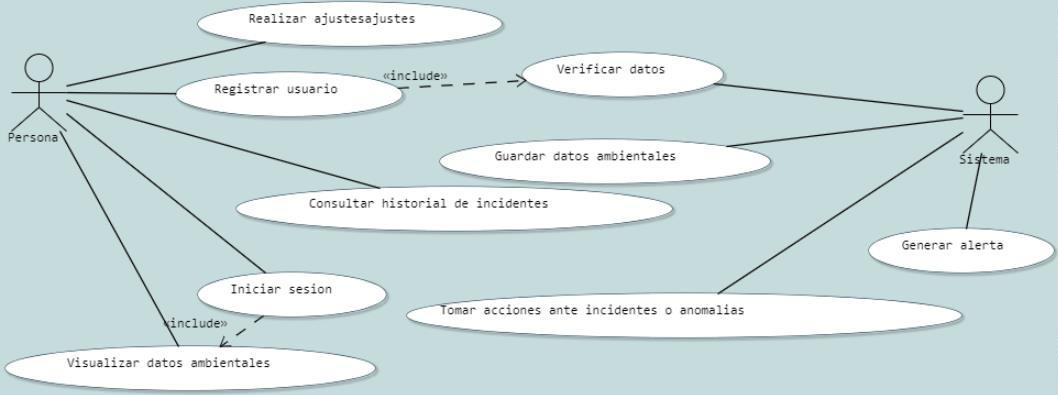
\includegraphics[width=407.5pt,height=152.15pt]{latexImage_e0fdadcfc09757a095d9e222496ab243.png}}
\end{picture}
\newpage
\begin{tikzpicture}[overlay]\path(0pt,0pt);\end{tikzpicture}
\begin{picture}(-5,0)(2.5,0)
\put(70.104,-71.03998){\fontsize{12}{1}\usefont{T1}{cmr}{m}{n}\selectfont\color{color_29791}Debido a que se especificó todos los detalles de los casos de uso, luego de generar el }
\put(70.104,-91.82001){\fontsize{12}{1}\usefont{T1}{cmr}{m}{n}\selectfont\color{color_29791}diagrama de clases no hubo necesidad de adaptar el diagrama de clases, se obtuvo un }
\put(70.104,-112.46){\fontsize{12}{1}\usefont{T1}{cmr}{m}{n}\selectfont\color{color_29791}diagrama de clases basado en las entidades que se mencionan en los casos de usos. }
\put(70.104,-141.26){\fontsize{12}{1}\usefont{T1}{cmr}{m}{n}\selectfont\color{color_29791}Además, se diseñó el dispositivo IoT con los componentes seleccionados en el menú de }
\put(70.104,-161.9){\fontsize{12}{1}\usefont{T1}{cmr}{m}{n}\selectfont\color{color_29791}la herramienta TDDT4IoTS, el cual genera parte del software que se usará en la web (Ver }
\put(70.104,-182.66){\fontsize{12}{1}\usefont{T1}{cmr}{m}{n}\selectfont\color{color_29791}Figura 3). Para compilar y ejecutar el código se utilizó el Arduino ide. Se realizaron }
\put(70.104,-203.3){\fontsize{12}{1}\usefont{T1}{cmr}{m}{n}\selectfont\color{color_29791}pruebas unitarias tras conectar los componentes para construir el dispositivo.  }
\put(70.104,-231.98){\fontsize{12}{1}\usefont{T1}{cmr}{m}{n}\selectfont\color{color_29791} }
\put(70.104,-260.69){\fontsize{12}{1}\usefont{T1}{cmr}{m}{n}\selectfont\color{color_29791} }
\put(70.104,-289.37){\fontsize{12}{1}\usefont{T1}{cmr}{m}{n}\selectfont\color{color_29791} }
\put(70.104,-318.17){\fontsize{12}{1}\usefont{T1}{cmr}{m}{n}\selectfont\color{color_29791} }
\put(70.104,-346.85){\fontsize{12}{1}\usefont{T1}{cmr}{m}{n}\selectfont\color{color_29791} }
\put(70.104,-375.53){\fontsize{12}{1}\usefont{T1}{cmr}{m}{n}\selectfont\color{color_29791} }
\put(70.104,-404.21){\fontsize{12}{1}\usefont{T1}{cmr}{m}{n}\selectfont\color{color_29791} }
\put(70.104,-432.91){\fontsize{12}{1}\usefont{T1}{cmr}{m}{n}\selectfont\color{color_29791} }
\put(70.104,-489.19){\fontsize{12}{1}\usefont{T1}{cmr}{m}{n}\selectfont\color{color_29791} }
\put(70.104,-517.87){\fontsize{12}{1}\usefont{T1}{cmr}{m}{n}\selectfont\color{color_29791}Durante las pruebas unitarias se conectó componente a componente para comprobar el }
\put(70.104,-538.63){\fontsize{12}{1}\usefont{T1}{cmr}{m}{n}\selectfont\color{color_29791}correcto funcionamiento y realizar la toma de datos que se almacenan en Firebase. Al }
\put(70.104,-559.27){\fontsize{12}{1}\usefont{T1}{cmr}{m}{n}\selectfont\color{color_29791}realizar las pruebas unitarias todas fueron satisfechas.  }
\put(70.104,-588.07){\fontsize{12}{1}\usefont{T1}{cmr}{m}{n}\selectfont\color{color_29791} }
\put(70.104,-616.78){\fontsize{12}{1}\usefont{T1}{cmr}{m}{n}\selectfont\color{color_29791} }
\put(70.104,-645.46){\fontsize{12}{1}\usefont{T1}{cmr}{m}{n}\selectfont\color{color_29791} }
\put(70.104,-674.14){\fontsize{12}{1}\usefont{T1}{cmr}{m}{n}\selectfont\color{color_29791} }
\put(70.104,-702.82){\fontsize{12}{1}\usefont{T1}{cmr}{m}{n}\selectfont\color{color_29791} }
\put(70.104,-731.496){\fontsize{12}{1}\usefont{T1}{cmr}{m}{n}\selectfont\color{color_29791} }
\put(139.5,-450.47){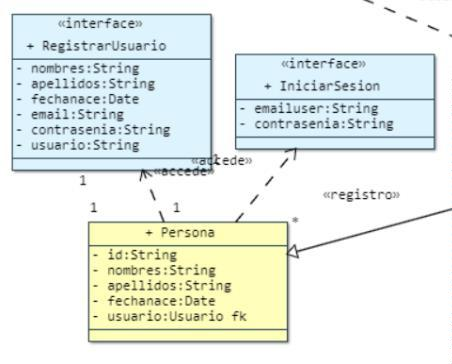
\includegraphics[width=267.15pt,height=214pt]{latexImage_7679a06c2598c55b79505827d47c3ac5.png}}
\end{picture}
\begin{tikzpicture}[overlay]
\path(0pt,0pt);
\filldraw[color_283006][even odd rule]
(-9.5501pt, -471.46pt) -- (550.5499pt, -471.46pt)
 -- (550.5499pt, -471.46pt)
 -- (550.5499pt, -451.11pt)
 -- (550.5499pt, -451.11pt)
 -- (-9.5501pt, -451.11pt) -- cycle
;
\begin{scope}
\clip
(-9.6pt, -471.55pt) -- (550.6801pt, -471.55pt)
 -- (550.6801pt, -471.55pt)
 -- (550.6801pt, -451.15pt)
 -- (550.6801pt, -451.15pt)
 -- (-9.6pt, -451.15pt) -- cycle
;
\begin{scope}
\clip
(-9.6pt, -471.55pt) -- (550.6801pt, -471.55pt)
 -- (550.6801pt, -471.55pt)
 -- (550.6801pt, -451.15pt)
 -- (550.6801pt, -451.15pt)
 -- (-9.6pt, -451.15pt) -- cycle
;
\end{scope}
\end{scope}
\end{tikzpicture}
\begin{picture}(-5,0)(2.5,0)
\put(159.86,-459.67){\fontsize{9}{1}\usefont{T1}{cmr}{m}{it}\selectfont\color{color_97849}Ilustración 4 Diagrama de clases generado con TDDM4IoTS }
\end{picture}
\newpage
\begin{tikzpicture}[overlay]\path(0pt,0pt);\end{tikzpicture}
\begin{picture}(-5,0)(2.5,0)
\put(88.1,-72.97998){\fontsize{14.04}{1}\usefont{T1}{cmr}{b}{n}\selectfont\color{color_29791}20. Diseño de interfaces }
\put(70.104,-94.46002){\fontsize{12}{1}\usefont{T1}{cmr}{m}{n}\selectfont\color{color_29791}A continuación, mostraremos las interfaces de la aplicación web }
\put(471.7,-310.61){\fontsize{12}{1}\usefont{T1}{cmr}{m}{n}\selectfont\color{color_29791} }
\put(230.21,-334.13){\fontsize{9}{1}\usefont{T1}{cmr}{m}{it}\selectfont\color{color_97849}Ilustración 5 Inicio de sesión }
\put(70.104,-357.05){\fontsize{12}{1}\usefont{T1}{cmr}{m}{n}\selectfont\color{color_29791}En la ilustración 5 podemos observar la pantalla inicial donde se podría Iniciar sesión y }
\put(70.104,-377.81){\fontsize{12}{1}\usefont{T1}{cmr}{m}{n}\selectfont\color{color_29791}acceder al inicio, en caso de que el usuario no este registrado también tendremos un }
\put(70.104,-398.45){\fontsize{12}{1}\usefont{T1}{cmr}{m}{n}\selectfont\color{color_29791}apartado de registro para agregar nuevos usuarios }
\put(70.104,-427.13){\fontsize{12}{1}\usefont{T1}{cmr}{m}{n}\selectfont\color{color_29791}  }
\put(70.104,-455.83){\fontsize{12}{1}\usefont{T1}{cmr}{m}{n}\selectfont\color{color_29791} }
\put(70.104,-484.63){\fontsize{12}{1}\usefont{T1}{cmr}{m}{n}\selectfont\color{color_29791} }
\put(70.104,-513.31){\fontsize{12}{1}\usefont{T1}{cmr}{m}{n}\selectfont\color{color_29791} }
\put(70.104,-541.99){\fontsize{12}{1}\usefont{T1}{cmr}{m}{n}\selectfont\color{color_29791} }
\put(70.104,-570.67){\fontsize{12}{1}\usefont{T1}{cmr}{m}{n}\selectfont\color{color_29791} }
\put(70.104,-599.35){\fontsize{12}{1}\usefont{T1}{cmr}{m}{n}\selectfont\color{color_29791} }
\put(70.104,-628.06){\fontsize{12}{1}\usefont{T1}{cmr}{m}{n}\selectfont\color{color_29791}En la ilustración 6 vemos la interfaz que solicita el correo y contraseña para agregar un }
\put(70.104,-648.82){\fontsize{12}{1}\usefont{T1}{cmr}{m}{n}\selectfont\color{color_29791}usuario nuevo, aquí se pedirá que se repita la contraseña para evitar que se agregue alguna }
\put(70.104,-669.46){\fontsize{12}{1}\usefont{T1}{cmr}{m}{n}\selectfont\color{color_29791}e}
\put(93.65,-310.6){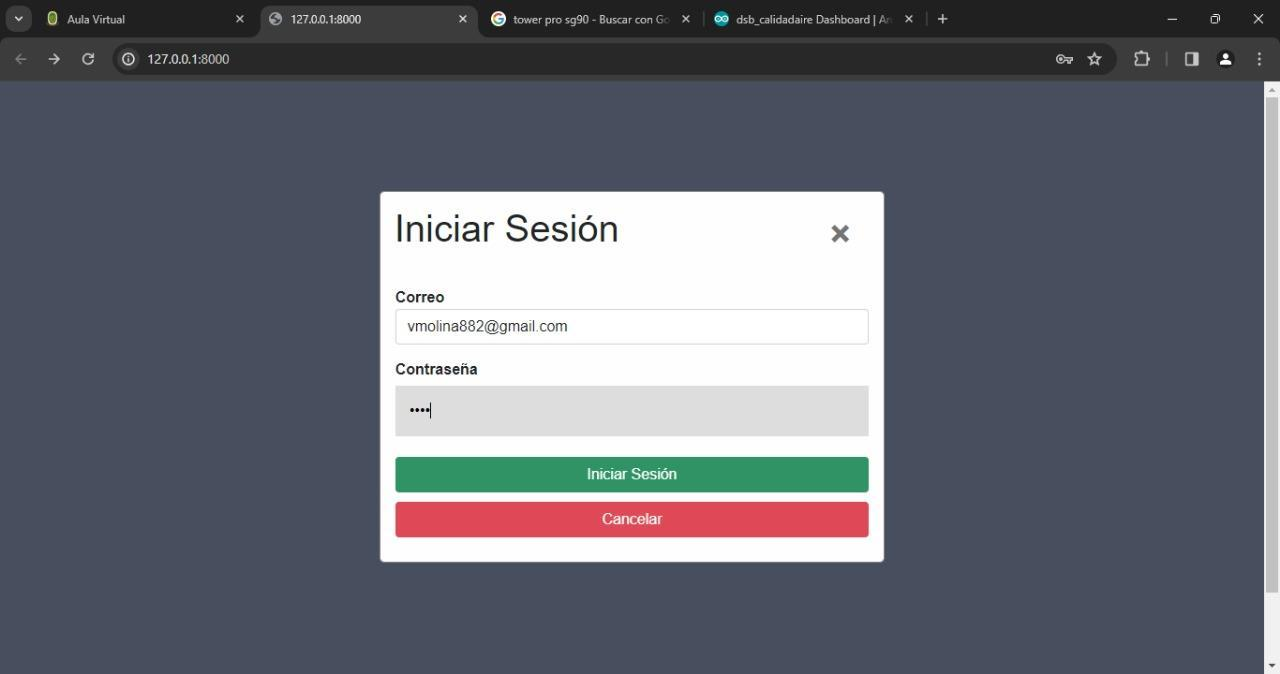
\includegraphics[width=377.41pt,height=198.6pt]{latexImage_18c4f2804ea6fe8b984159f507c46bb3.png}}
\put(117.7,-597.8){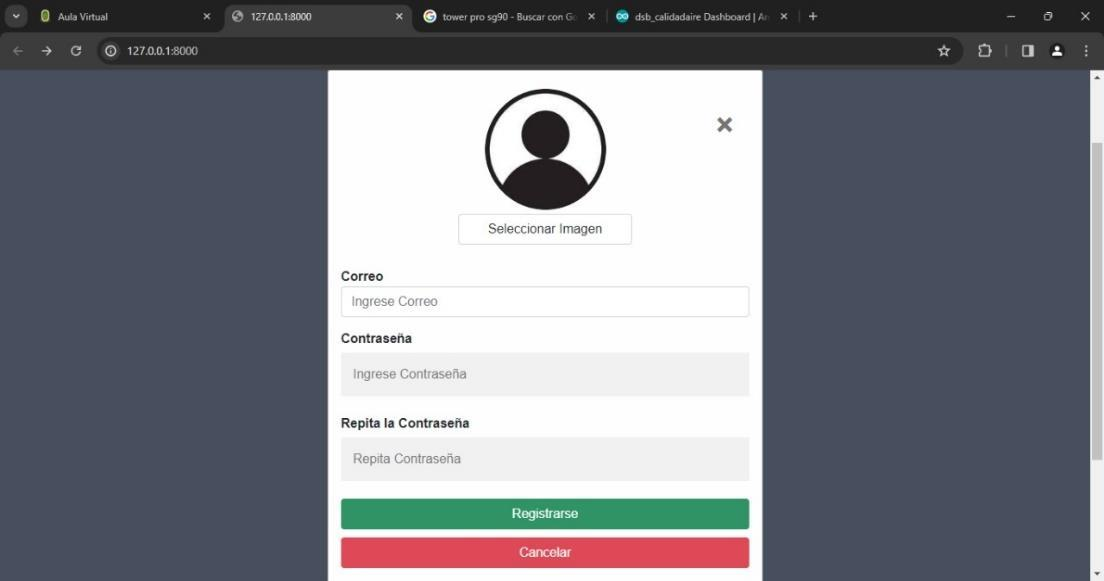
\includegraphics[width=360.95pt,height=190.1pt]{latexImage_1d487e42d8b512ec4e300129f38fb260.png}}
\end{picture}
\begin{tikzpicture}[overlay]
\path(0pt,0pt);
\filldraw[color_283006][even odd rule]
(117.7pt, -598.24pt) -- (478.65pt, -598.24pt)
 -- (478.65pt, -598.24pt)
 -- (478.65pt, -577.89pt)
 -- (478.65pt, -577.89pt)
 -- (117.7pt, -577.89pt) -- cycle
;
\begin{scope}
\clip
(117.74pt, -598.27pt) -- (478.77pt, -598.27pt)
 -- (478.77pt, -598.27pt)
 -- (478.77pt, -577.99pt)
 -- (478.77pt, -577.99pt)
 -- (117.74pt, -577.99pt) -- cycle
;
\begin{scope}
\clip
(117.74pt, -598.27pt) -- (478.77pt, -598.27pt)
 -- (478.77pt, -598.27pt)
 -- (478.77pt, -577.99pt)
 -- (478.77pt, -577.99pt)
 -- (117.74pt, -577.99pt) -- cycle
;
\end{scope}
\end{scope}
\end{tikzpicture}
\begin{picture}(-5,0)(2.5,0)
\put(236.93,-586.51){\fontsize{9}{1}\usefont{T1}{cmr}{m}{it}\selectfont\color{color_97849}Ilustración 6 Registro de usuarios }
\end{picture}
\newpage
\begin{tikzpicture}[overlay]\path(0pt,0pt);\end{tikzpicture}
\begin{picture}(-5,0)(2.5,0)
\put(475.78,-273.65){\fontsize{12}{1}\usefont{T1}{cmr}{m}{n}\selectfont\color{color_29791} }
\put(230.57,-297.05){\fontsize{9}{1}\usefont{T1}{cmr}{m}{it}\selectfont\color{color_97849}Ilustración 7 Menú principal }
\put(495.34,-532.87){\fontsize{12}{1}\usefont{T1}{cmr}{m}{n}\selectfont\color{color_29791} }
\put(212.69,-556.27){\fontsize{9}{1}\usefont{T1}{cmr}{m}{it}\selectfont\color{color_97849}Ilustración 8 Monitoreo en tiempo real }
\put(70.104,-579.31){\fontsize{12}{1}\usefont{T1}{cmr}{m}{n}\selectfont\color{color_29791}En las figuras 7 y 8 podemos observar las interfaces que mas se utilizaran las cuales son }
\put(70.104,-594.19){\fontsize{12}{1}\usefont{T1}{cmr}{m}{n}\selectfont\color{color_29791}el menú inicio y el modulo de tiempo real, en este ultimo podemos ver en gráficos las }
\put(70.104,-609.1){\fontsize{12}{1}\usefont{T1}{cmr}{m}{n}\selectfont\color{color_29791}estadísticas actuales que se envían por el sensor. }
\put(88.1,-643.9){\fontsize{14.04}{1}\usefont{T1}{cmr}{b}{n}\selectfont\color{color_29791}21. Diagrama de clases }
\put(70.104,-665.38){\fontsize{12}{1}\usefont{T1}{cmr}{m}{n}\selectfont\color{color_29791}Durante la etapa de refinamiento, se agregó una clase adicional y se definieron los }
\put(70.104,-686.02){\fontsize{12}{1}\usefont{T1}{cmr}{m}{n}\selectfont\color{color_29791}métodos faltantes en los casos de uso. En la Fig. 9, se presenta el diagrama de clases }
\put(70.104,-706.78){\fontsize{12}{1}\usefont{T1}{cmr}{m}{n}\selectfont\color{color_29791}re}
\put(70.05,-273.58){
\includegraphics[width=405.64pt,height=213.65pt]{latexImage_e8eade6ac2373bf453fef5bdb3d80668.png}}
\put(70.05,-532.78){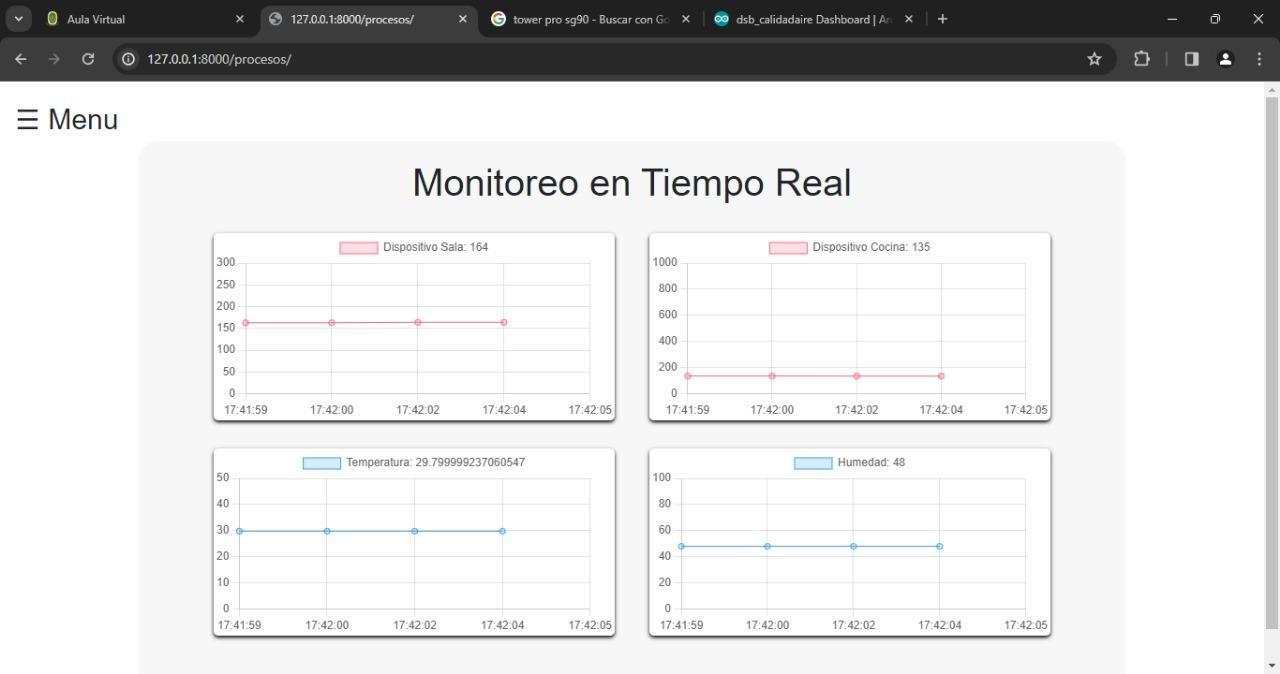
\includegraphics[width=425.2pt,height=223.95pt]{latexImage_8bf17ba38e2cddee45493efa0f8b0631.png}}
\end{picture}
\newpage
\begin{tikzpicture}[overlay]\path(0pt,0pt);\end{tikzpicture}
\begin{picture}(-5,0)(2.5,0)
\put(70.104,-71.03998){\fontsize{12}{1}\usefont{T1}{cmr}{m}{n}\selectfont\color{color_29791}A continuación, se mostrará el diagrama de clases. }
\put(460.54,-99.85999){\fontsize{12}{1}\usefont{T1}{cmr}{m}{n}\selectfont\color{color_29791} }
\put(460.54,-122.66){\fontsize{12}{1}\usefont{T1}{cmr}{m}{n}\selectfont\color{color_29791} }
\put(460.54,-145.58){\fontsize{12}{1}\usefont{T1}{cmr}{m}{n}\selectfont\color{color_29791} }
\put(460.54,-168.5){\fontsize{12}{1}\usefont{T1}{cmr}{m}{n}\selectfont\color{color_29791} }
\put(460.54,-191.42){\fontsize{12}{1}\usefont{T1}{cmr}{m}{n}\selectfont\color{color_29791} }
\put(84.264,-283.97){\fontsize{15.96}{1}\usefont{T1}{cmr}{b}{n}\selectfont\color{color_29791}22. Implementación de Hardware y Software  }
\put(239.57,-541.99){\fontsize{9}{1}\usefont{T1}{cmr}{m}{it}\selectfont\color{color_97849}Ilustración 10 prototipo }
\put(70.104,-565.03){\fontsize{12}{1}\usefont{T1}{cmr}{m}{n}\selectfont\color{color_29791}Durante el proceso de implementación de hardware y software se lograron conectar los }
\put(70.104,-585.79){\fontsize{12}{1}\usefont{T1}{cmr}{m}{n}\selectfont\color{color_29791}sensores MQ2 Y MQ135  a sus respectivos módulos ESP8266  y estos directamente a la }
\put(70.104,-606.43){\fontsize{12}{1}\usefont{T1}{cmr}{m}{n}\selectfont\color{color_29791}Protoboard para que de esta manera la información tomada por los sensores sea subida a }
\put(70.104,-627.22){\fontsize{12}{1}\usefont{T1}{cmr}{m}{n}\selectfont\color{color_29791}ARDUINO CLOUDE y de alli sea enviada a FIREBASE para que finalmente sea  }
\put(70.104,-647.86){\fontsize{12}{1}\usefont{T1}{cmr}{m}{n}\selectfont\color{color_29791}presentada en lainterfaz que el usuario visualiza tanto en la aplicación móvil como en la }
\put(70.104,-668.5){\fontsize{12}{1}\usefont{T1}{cmr}{m}{n}\selectfont\color{color_29791}web. }
\put(70.104,-697.3){\fontsize{12}{1}\usefont{T1}{cmr}{m}{n}\selectfont\color{color_29791} }
\put(70.05,-533.46){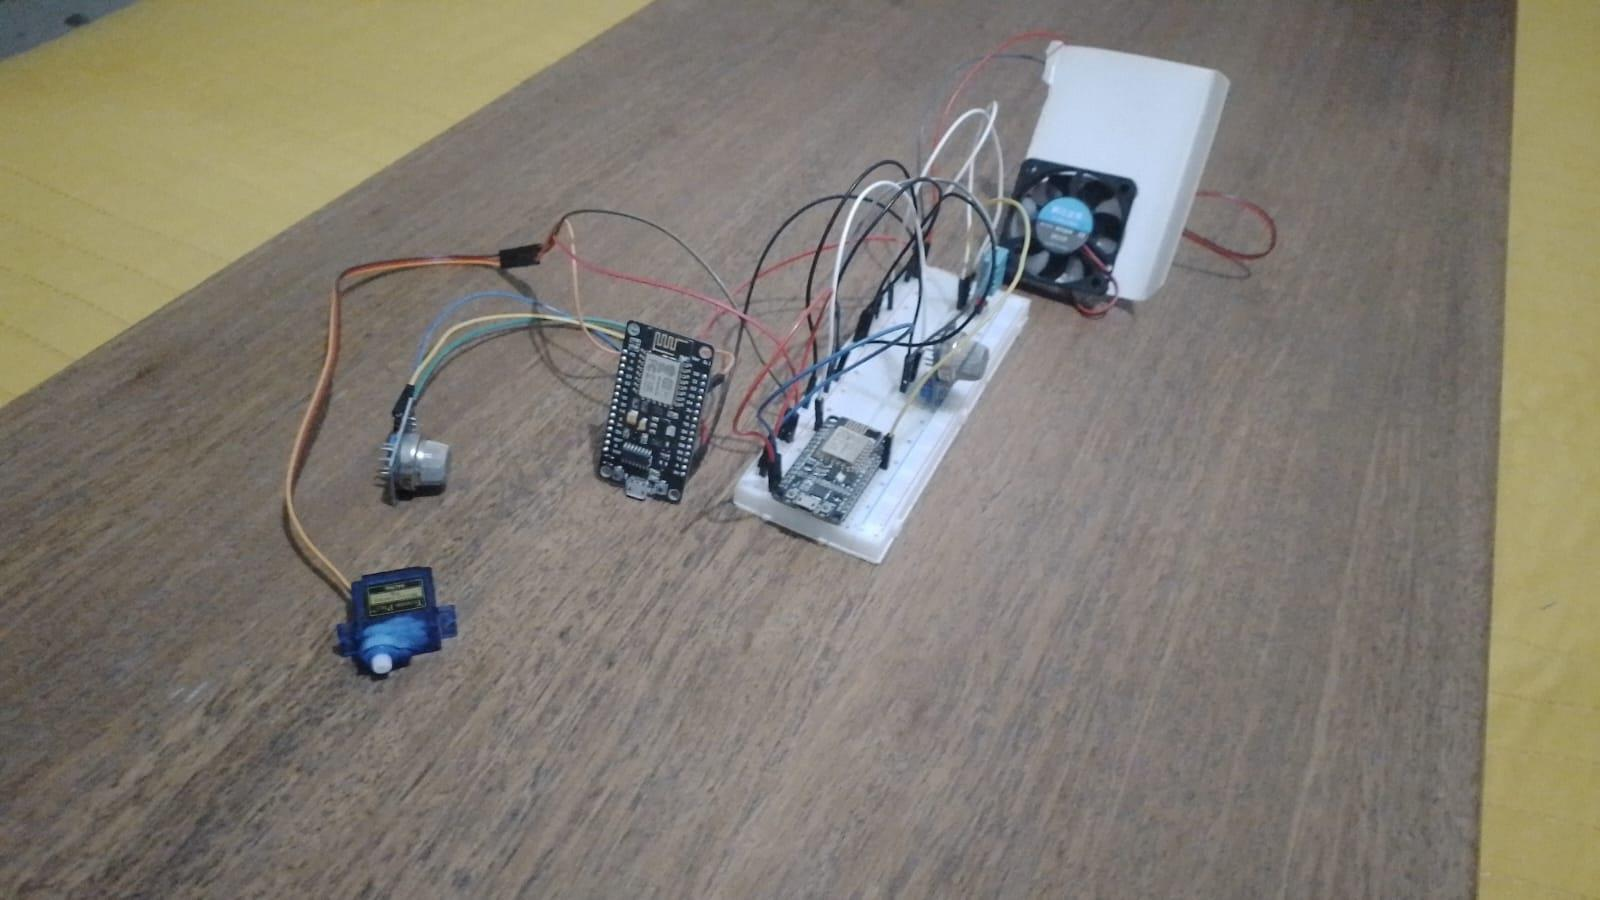
\includegraphics[width=425.2pt,height=239.2pt]{latexImage_3206c243b72f303438f9e0c1f31ef41f.png}}
\end{picture}
\begin{tikzpicture}[overlay]
\path(0pt,0pt);
\filldraw[color_283006][even odd rule]
(5.65pt, -236.59pt) -- (565.75pt, -236.59pt)
 -- (565.75pt, -236.59pt)
 -- (565.75pt, -216.2401pt)
 -- (565.75pt, -216.2401pt)
 -- (5.65pt, -216.2401pt) -- cycle
;
\begin{scope}
\clip
(5.639999pt, -236.66pt) -- (565.92pt, -236.66pt)
 -- (565.92pt, -236.66pt)
 -- (565.92pt, -216.2599pt)
 -- (565.92pt, -216.2599pt)
 -- (5.639999pt, -216.2599pt) -- cycle
;
\begin{scope}
\clip
(5.639999pt, -236.66pt) -- (565.92pt, -236.66pt)
 -- (565.92pt, -236.66pt)
 -- (565.92pt, -216.2599pt)
 -- (565.92pt, -216.2599pt)
 -- (5.639999pt, -216.2599pt) -- cycle
;
\end{scope}
\end{scope}
\end{tikzpicture}
\begin{picture}(-5,0)(2.5,0)
\put(157.46,-224.78){\fontsize{9}{1}\usefont{T1}{cmr}{m}{it}\selectfont\color{color_97849}Ilu}
\put(87,-257.53){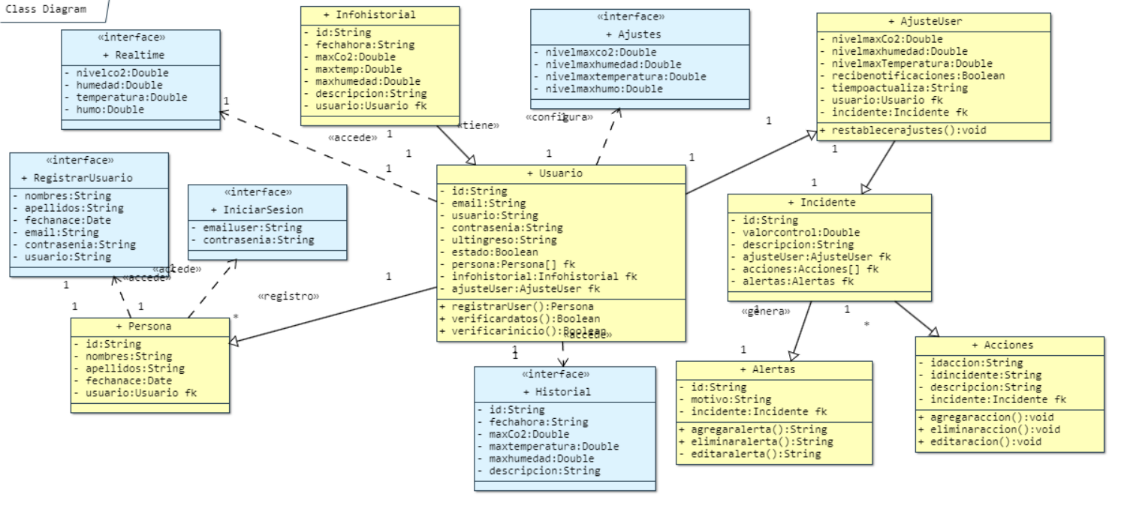
\includegraphics[width=366.5pt,height=168.4pt]{latexImage_751d33cdf5cf7464590a95f0a81e8a77.png}}
\end{picture}
\newpage
\begin{tikzpicture}[overlay]\path(0pt,0pt);\end{tikzpicture}
\begin{picture}(-5,0)(2.5,0)
\put(88.1,-72.97998){\fontsize{14.04}{1}\usefont{T1}{cmr}{b}{n}\selectfont\color{color_29791}23. Resultados y discusión }
\put(70.104,-94.46002){\fontsize{12}{1}\usefont{T1}{cmr}{m}{n}\selectfont\color{color_29791}Tras la implementación del SafeAir Monitor, se observó una mejora significativa en la }
\put(70.104,-115.22){\fontsize{12}{1}\usefont{T1}{cmr}{m}{n}\selectfont\color{color_29791}calidad del aire en espacios interiores. Los niveles de contaminantes como CO2, }
\put(70.104,-135.86){\fontsize{12}{1}\usefont{T1}{cmr}{m}{n}\selectfont\color{color_29791}partículas suspendidas y compuestos orgánicos volátiles se mantuvieron dentro de los }
\put(70.104,-156.62){\fontsize{12}{1}\usefont{T1}{cmr}{m}{n}\selectfont\color{color_29791}límites recomendados, lo que contribuyó a un ambiente más saludable y seguro para los }
\put(70.104,-177.26){\fontsize{12}{1}\usefont{T1}{cmr}{m}{n}\selectfont\color{color_29791}ocupantes del hogar. La eficacia del sistema en la detección temprana de contaminantes }
\put(70.104,-198.02){\fontsize{12}{1}\usefont{T1}{cmr}{m}{n}\selectfont\color{color_29791}y en la activación automática de medidas correctivas durante las pruebas en entornos }
\put(70.104,-218.66){\fontsize{12}{1}\usefont{T1}{cmr}{m}{n}\selectfont\color{color_29791}reales demostró su capacidad para mantener la calidad del aire en niveles óptimos, }
\put(70.104,-239.42){\fontsize{12}{1}\usefont{T1}{cmr}{m}{n}\selectfont\color{color_29791}evitando riesgos para la salud de los residentes. Además, se comprobó que el SafeAir }
\put(70.104,-260.09){\fontsize{12}{1}\usefont{T1}{cmr}{m}{n}\selectfont\color{color_29791}Monitor era capaz de manejar eficientemente un aumento en el número de sensores y }
\put(70.104,-280.85){\fontsize{12}{1}\usefont{T1}{cmr}{m}{n}\selectfont\color{color_29791}usuarios, garantizando un monitoreo continuo y personalizado para cada hogar, lo que es }
\put(70.104,-301.49){\fontsize{12}{1}\usefont{T1}{cmr}{m}{n}\selectfont\color{color_29791}fundamental para asegurar su efectividad a largo plazo en diferentes entornos domésticos. }
\put(70.104,-330.17){\fontsize{12}{1}\usefont{T1}{cmr}{m}{n}\selectfont\color{color_29791}La implementación del SafeAir Monitor no solo tuvo un impacto inmediato en la calidad }
\put(70.104,-350.93){\fontsize{12}{1}\usefont{T1}{cmr}{m}{n}\selectfont\color{color_29791}del aire interior, sino que también se proyecta como una inversión a largo plazo en la }
\put(70.104,-371.57){\fontsize{12}{1}\usefont{T1}{cmr}{m}{n}\selectfont\color{color_29791}salud y bienestar de los residentes. La prevención de enfermedades respiratorias y alergias }
\put(70.104,-392.33){\fontsize{12}{1}\usefont{T1}{cmr}{m}{n}\selectfont\color{color_29791}relacionadas con la mala calidad del aire puede resultar en ahorros significativos en costos }
\put(70.104,-412.97){\fontsize{12}{1}\usefont{T1}{cmr}{m}{n}\selectfont\color{color_29791}de atención médica y mejorar la calidad de vida en general. Considerando el avance }
\put(70.104,-433.75){\fontsize{12}{1}\usefont{T1}{cmr}{m}{n}\selectfont\color{color_29791}constante de la tecnología IoT y la domótica, el SafeAir Monitor tiene el potencial de }
\put(70.104,-454.39){\fontsize{12}{1}\usefont{T1}{cmr}{m}{n}\selectfont\color{color_29791}integrarse con otros dispositivos inteligentes en el hogar para una gestión más eficiente y }
\put(70.104,-475.15){\fontsize{12}{1}\usefont{T1}{cmr}{m}{n}\selectfont\color{color_29791}automatizada del ambiente interior. Esta sinergia tecnológica podría ofrecer nuevas }
\put(70.104,-495.79){\fontsize{12}{1}\usefont{T1}{cmr}{m}{n}\selectfont\color{color_29791}funcionalidades y beneficios para los usuarios, como la optimización energética y la }
\put(70.104,-516.55){\fontsize{12}{1}\usefont{T1}{cmr}{m}{n}\selectfont\color{color_29791}personalización de las preferencias de calidad del aire. Al promover la conciencia sobre }
\put(70.104,-537.19){\fontsize{12}{1}\usefont{T1}{cmr}{m}{n}\selectfont\color{color_29791}la importancia de la calidad del aire en el hogar, el SafeAir Monitor no solo beneficia a }
\put(70.104,-557.95){\fontsize{12}{1}\usefont{T1}{cmr}{m}{n}\selectfont\color{color_29791}los usuarios directos, sino que también contribuye a la sensibilización sobre la }
\put(70.104,-578.59){\fontsize{12}{1}\usefont{T1}{cmr}{m}{n}\selectfont\color{color_29791}contaminación del aire en espacios interiores a nivel comunitario. Esta sensibilización }
\put(70.104,-599.35){\fontsize{12}{1}\usefont{T1}{cmr}{m}{n}\selectfont\color{color_29791}puede llevar a cambios de comportamiento y hábitos más saludables, impactando }
\put(70.104,-620.02){\fontsize{12}{1}\usefont{T1}{cmr}{m}{n}\selectfont\color{color_29791}positivamente en la salud pública y en la reducción de la huella ambiental. }
\put(70.104,-648.7){\fontsize{12}{1}\usefont{T1}{cmr}{m}{n}\selectfont\color{color_29791} }
\put(70.104,-677.38){\fontsize{12}{1}\usefont{T1}{cmr}{m}{n}\selectfont\color{color_29791} }
\put(70.104,-706.06){\fontsize{12}{1}\usefont{T1}{cmr}{m}{n}\selectfont\color{color_29791} }
\end{picture}
\newpage
\begin{tikzpicture}[overlay]\path(0pt,0pt);\end{tikzpicture}
\begin{picture}(-5,0)(2.5,0)
\put(88.1,-72.97998){\fontsize{14.04}{1}\usefont{T1}{cmr}{b}{n}\selectfont\color{color_29791}24. Conclusiones y recomendaciones }
\put(70.104,-94.46002){\fontsize{12}{1}\usefont{T1}{cmr}{m}{n}\selectfont\color{color_29791}Tras la implementación y evaluación del Sistema Inteligente de Monitoreo y Control de }
\put(70.104,-115.22){\fontsize{12}{1}\usefont{T1}{cmr}{m}{n}\selectfont\color{color_29791}Calidad del Aire SafeAir Monitor, se ha observado un impacto positivo y significativo en }
\put(70.104,-135.86){\fontsize{12}{1}\usefont{T1}{cmr}{m}{n}\selectfont\color{color_29791}la calidad del aire en espacios interiores. La capacidad del sistema para detectar y alertar }
\put(70.104,-156.62){\fontsize{12}{1}\usefont{T1}{cmr}{m}{n}\selectfont\color{color_29791}sobre niveles elevados de contaminantes, así como para activar medidas correctivas }
\put(70.104,-177.26){\fontsize{12}{1}\usefont{T1}{cmr}{m}{n}\selectfont\color{color_29791}automáticas, ha sido fundamental para mantener un ambiente interior saludable y seguro. }
\put(70.104,-198.02){\fontsize{12}{1}\usefont{T1}{cmr}{m}{n}\selectfont\color{color_29791}Durante las pruebas y validaciones en entornos reales, se constató la efectividad del }
\put(70.104,-218.66){\fontsize{12}{1}\usefont{T1}{cmr}{m}{n}\selectfont\color{color_29791}SafeAir Monitor en detectar y prevenir la contaminación del aire en espacios interiores. }
\put(70.104,-239.42){\fontsize{12}{1}\usefont{T1}{cmr}{m}{n}\selectfont\color{color_29791}La respuesta automática del sistema, como la activación de la ventilación en caso de }
\put(70.104,-260.09){\fontsize{12}{1}\usefont{T1}{cmr}{m}{n}\selectfont\color{color_29791}niveles elevados de contaminantes, ha demostrado ser crucial para garantizar un aire }
\put(70.104,-280.85){\fontsize{12}{1}\usefont{T1}{cmr}{m}{n}\selectfont\color{color_29791}limpio y libre de contaminantes en los hogares. Además, la evaluación de la interfaz de }
\put(70.104,-301.49){\fontsize{12}{1}\usefont{T1}{cmr}{m}{n}\selectfont\color{color_29791}usuario ha destacado su accesibilidad y facilidad de uso, contribuyendo a una experiencia }
\put(70.104,-322.25){\fontsize{12}{1}\usefont{T1}{cmr}{m}{n}\selectfont\color{color_29791}positiva por parte de los usuarios.  }
\put(70.104,-350.93){\fontsize{12}{1}\usefont{T1}{cmr}{m}{n}\selectfont\color{color_29791}Se recomienda la expansión y promoción del SafeAir Monitor como una solución }
\put(70.104,-371.57){\fontsize{12}{1}\usefont{T1}{cmr}{m}{n}\selectfont\color{color_29791}innovadora y preventiva para mejorar la calidad de vida en entornos domésticos. Se }
\put(70.104,-392.33){\fontsize{12}{1}\usefont{T1}{cmr}{m}{n}\selectfont\color{color_29791}sugiere la colaboración con entidades gubernamentales y organizaciones de salud para }
\put(70.104,-412.97){\fontsize{12}{1}\usefont{T1}{cmr}{m}{n}\selectfont\color{color_29791}fomentar la adopción de sistemas de monitoreo de calidad del aire en hogares, }
\put(70.104,-433.75){\fontsize{12}{1}\usefont{T1}{cmr}{m}{n}\selectfont\color{color_29791}especialmente aquellos con poblaciones vulnerables como niños, ancianos y personas con }
\put(70.104,-454.39){\fontsize{12}{1}\usefont{T1}{cmr}{m}{n}\selectfont\color{color_29791}condiciones médicas preexistentes. Es fundamental seguir investigando y desarrollando }
\put(70.104,-475.15){\fontsize{12}{1}\usefont{T1}{cmr}{m}{n}\selectfont\color{color_29791}nuevas funcionalidades para el SafeAir Monitor, con el objetivo de mejorar su eficacia y }
\put(70.104,-495.79){\fontsize{12}{1}\usefont{T1}{cmr}{m}{n}\selectfont\color{color_29791}adaptabilidad a diferentes entornos domésticos. Se propone la integración del SafeAir }
\put(70.104,-516.55){\fontsize{12}{1}\usefont{T1}{cmr}{m}{n}\selectfont\color{color_29791}Monitor con otros dispositivos inteligentes en el hogar para una gestión más eficiente y }
\put(70.104,-537.19){\fontsize{12}{1}\usefont{T1}{cmr}{m}{n}\selectfont\color{color_29791}automatizada del ambiente interior, lo que podría ofrecer beneficios adicionales a los }
\put(70.104,-557.95){\fontsize{12}{1}\usefont{T1}{cmr}{m}{n}\selectfont\color{color_29791}usuarios, como la optimización energética y la personalización de las preferencias de }
\put(70.104,-578.59){\fontsize{12}{1}\usefont{T1}{cmr}{m}{n}\selectfont\color{color_29791}calidad del aire. Asimismo, se destaca la importancia de continuar educando a la }
\put(70.104,-599.35){\fontsize{12}{1}\usefont{T1}{cmr}{m}{n}\selectfont\color{color_29791}comunidad sobre los beneficios de mantener un ambiente interior saludable y la }
\put(70.104,-620.02){\fontsize{12}{1}\usefont{T1}{cmr}{m}{n}\selectfont\color{color_29791}relevancia de la calidad del aire en la salud humana, con el fin de promover prácticas }
\put(70.104,-640.66){\fontsize{12}{1}\usefont{T1}{cmr}{m}{n}\selectfont\color{color_29791}sostenibles y saludables en los hogares. }
\put(70.104,-669.46){\fontsize{12}{1}\usefont{T1}{cmr}{m}{n}\selectfont\color{color_29791} }
\put(70.104,-698.14){\fontsize{12}{1}\usefont{T1}{cmr}{m}{n}\selectfont\color{color_29791} }
\put(70.104,-726.82){\fontsize{12}{1}\usefont{T1}{cmr}{m}{n}\selectfont\color{color_29791} }
\end{picture}
\newpage
\begin{tikzpicture}[overlay]\path(0pt,0pt);\end{tikzpicture}
\begin{picture}(-5,0)(2.5,0)
\put(88.1,-72.97998){\fontsize{14.04}{1}\usefont{T1}{cmr}{b}{n}\selectfont\color{color_29791}25. Bibliografía  }
\put(70.104,-94.46002){\fontsize{12}{1}\usefont{T1}{cmr}{m}{n}\selectfont\color{color_29791}[1] J. M. Corchado et al., “Development and Assessment of an Indoor Air Quality }
\put(102.14,-115.22){\fontsize{12}{1}\usefont{T1}{cmr}{m}{n}\selectfont\color{color_29791}Control IoT-Based System,” Electronics 2023, Vol. 12, Page 608, vol. 12, no. 3, p. }
\put(102.14,-135.86){\fontsize{12}{1}\usefont{T1}{cmr}{m}{n}\selectfont\color{color_29791}608, Jan. 2023, doi: 10.3390/ELECTRONICS12030608. }
\put(70.104,-164.54){\fontsize{12}{1}\usefont{T1}{cmr}{m}{n}\selectfont\color{color_29791}[2] A. M. Odeh and I. Ishaq, “The Implementation of a Smart Home Security Network }
\put(102.14,-185.3){\fontsize{12}{1}\usefont{T1}{cmr}{m}{n}\selectfont\color{color_29791}Using Internet of Things (IoT) System,” Lecture Notes in Networks and Systems, }
\put(102.14,-205.94){\fontsize{12}{1}\usefont{T1}{cmr}{m}{n}\selectfont\color{color_29791}vol. 579, pp. 369–385, 2023, doi: 10.1007/978-981-19-7663-6\_35/COVER. }
\put(70.104,-234.62){\fontsize{12}{1}\usefont{T1}{cmr}{m}{n}\selectfont\color{color_29791}[3] L. Pang, C. Luo, and W. Pan, “Research on the impact of indoor control quality }
\put(102.14,-255.41){\fontsize{12}{1}\usefont{T1}{cmr}{m}{n}\selectfont\color{color_29791}monitoring based on Internet of Things,” IEEE Access, 2023, doi: }
\put(102.14,-276.05){\fontsize{12}{1}\usefont{T1}{cmr}{m}{n}\selectfont\color{color_29791}10.1109/ACCESS.2023.3336706. }
\put(70.104,-304.85){\fontsize{12}{1}\usefont{T1}{cmr}{m}{n}\selectfont\color{color_29791}[4] M. Zhou, A. M. Abdulghani, M. A. Imran, and Q. H. Abbasi, “Internet of Things }
\put(102.14,-325.49){\fontsize{12}{1}\usefont{T1}{cmr}{m}{n}\selectfont\color{color_29791}(IoT) Enabled Smart Indoor Air Quality Monitoring System,” ACM International }
\put(102.14,-346.25){\fontsize{12}{1}\usefont{T1}{cmr}{m}{it}\selectfont\color{color_29791}Conference Proceeding Series, pp. 89–93, Apr. 2020, doi: }
\put(102.14,-366.89){\fontsize{12}{1}\usefont{T1}{cmr}{m}{n}\selectfont\color{color_29791}10.1145/3398329.3398342. }
\put(70.104,-395.57){\fontsize{12}{1}\usefont{T1}{cmr}{m}{n}\selectfont\color{color_29791}[5] K. Rastogi and D. Lohani, “Context-aware IoT-enabled framework to analyse and }
\put(102.14,-416.33){\fontsize{12}{1}\usefont{T1}{cmr}{m}{n}\selectfont\color{color_29791}predict indoor air quality,” Intelligent Systems with Applications, vol. 16, p. }
\put(102.14,-436.99){\fontsize{12}{1}\usefont{T1}{cmr}{m}{n}\selectfont\color{color_29791}200132, Nov. 2022, doi: 10.1016/J.ISWA.2022.200132. }
\put(70.104,-465.67){\fontsize{12}{1}\usefont{T1}{cmr}{m}{n}\selectfont\color{color_29791}[6] J. Pantelic, Y. J. Son, B. Staven, and Q. Liu, “Cooking emission control with IoT }
\put(102.14,-486.43){\fontsize{12}{1}\usefont{T1}{cmr}{m}{n}\selectfont\color{color_29791}sensors and connected air quality interventions for smart and healthy homes: }
\put(102.14,-507.07){\fontsize{12}{1}\usefont{T1}{cmr}{m}{n}\selectfont\color{color_29791}Evaluation of effectiveness and energy consumption,” Energy Build, vol. 286, p. }
\put(102.14,-527.83){\fontsize{12}{1}\usefont{T1}{cmr}{m}{n}\selectfont\color{color_29791}112932, May 2023, doi: 10.1016/J.ENBUILD.2023.112932. }
\put(70.104,-556.51){\fontsize{12}{1}\usefont{T1}{cmr}{m}{n}\selectfont\color{color_29791}[7] J. Wang et al., “Quantifying the dynamic characteristics of indoor air pollution }
\put(102.14,-577.15){\fontsize{12}{1}\usefont{T1}{cmr}{m}{n}\selectfont\color{color_29791}using real-time sensors: Current status and future implication,” Environ Int, vol. }
\put(102.14,-597.91){\fontsize{12}{1}\usefont{T1}{cmr}{m}{n}\selectfont\color{color_29791}175, p. 107934, May 2023, doi: 10.1016/J.ENVINT.2023.107934. }
\put(70.104,-626.62){\fontsize{12}{1}\usefont{T1}{cmr}{m}{n}\selectfont\color{color_29791}[8] “Display 16x2 Alfanumérico (QAPASS / 1602A) - Wassermatic.” Accessed: Jan. }
\put(102.14,-647.38){\fontsize{12}{1}\usefont{T1}{cmr}{m}{n}\selectfont\color{color_29791}29, 2024. [Online]. Available: }
\put(102.14,-668.02){\fontsize{12}{1}\usefont{T1}{cmr}{m}{n}\selectfont\color{color_29791}https://www.wassermatic.com.mx/index.php/productos/productoDetalle/13 }
\put(70.104,-696.7){\fontsize{12}{1}\usefont{T1}{cmr}{m}{n}\selectfont\color{color_29791}[9] “Modulo WiFi ESP8266 NodeMCU.” Accessed: Jan. 29, 2024. [Online]. }
\put(102.14,-717.46){\fontsize{12}{1}\usefont{T1}{cmr}{m}{n}\selectfont\color{color_29791}Available: https://tecmikro.com/modulos-shields/598-modulo-wifi-esp8266-}
\put(102.14,-738.096){\fontsize{12}{1}\usefont{T1}{cmr}{m}{n}\selectfont\color{color_29791}nodemcu.html }
\end{picture}
\newpage
\begin{tikzpicture}[overlay]\path(0pt,0pt);\end{tikzpicture}
\begin{picture}(-5,0)(2.5,0)
\put(70.104,-71.03998){\fontsize{12}{1}\usefont{T1}{cmr}{m}{n}\selectfont\color{color_29791}[10] “Servomotor SG90 RC 9g - UNIT Electronics Arduino Micro Servo.” Accessed: }
\put(102.14,-91.82001){\fontsize{12}{1}\usefont{T1}{cmr}{m}{n}\selectfont\color{color_29791}Jan. 29, 2024. [Online]. Available: https://uelectronics.com/producto/servomotor-}
\put(102.14,-112.46){\fontsize{12}{1}\usefont{T1}{cmr}{m}{n}\selectfont\color{color_29791}sg90-rc-9g/ }
\put(70.104,-141.26){\fontsize{12}{1}\usefont{T1}{cmr}{m}{n}\selectfont\color{color_29791}[11] “ARDUINO – Blog de Tecnologías.” Accessed: Jan. 29, 2024. [Online]. Available: }
\put(102.14,-161.9){\fontsize{12}{1}\usefont{T1}{cmr}{m}{n}\selectfont\color{color_29791}https://www3.gobiernodecanarias.org/medusa/ecoblog/rsuagued/arduino/ }
\put(70.104,-190.58){\fontsize{12}{1}\usefont{T1}{cmr}{m}{n}\selectfont\color{color_29791}[12] “Qué es Visual Studio Code y qué ventajas ofrece | OpenWebinars.” Accessed: Jan. }
\put(102.14,-211.34){\fontsize{12}{1}\usefont{T1}{cmr}{m}{n}\selectfont\color{color_29791}29, 2024. [Online]. Available: https://openwebinars.net/blog/que-es-visual-studio-}
\put(102.14,-231.98){\fontsize{12}{1}\usefont{T1}{cmr}{m}{n}\selectfont\color{color_29791}code-y-que-ventajas-ofrece/ }
\put(70.104,-260.93){\fontsize{12}{1}\usefont{T1}{cmr}{m}{n}\selectfont\color{color_29791}[13] “▷ Android Studio el entorno de desarrollo oficial de Android.” Accessed: Jan. 29, }
\put(102.14,-281.81){\fontsize{12}{1}\usefont{T1}{cmr}{m}{n}\selectfont\color{color_29791}2024. [Online]. Available: https://scoreapps.com/blog/android-studio/ }
\put(70.104,-310.49){\fontsize{12}{1}\usefont{T1}{cmr}{m}{n}\selectfont\color{color_29791}[14] “Arduino Pro – camino fácil y poco convencional hacia el éxito de las aplicaciones }
\put(102.14,-331.25){\fontsize{12}{1}\usefont{T1}{cmr}{m}{n}\selectfont\color{color_29791}IoT | Distribuidor de componentes electrónicos. Tienda en línea: Transfer Multisort }
\put(102.14,-351.89){\fontsize{12}{1}\usefont{T1}{cmr}{m}{n}\selectfont\color{color_29791}Elektronik.” Accessed: Jan. 29, 2024. [Online]. Available: }
\put(102.14,-372.65){\fontsize{12}{1}\usefont{T1}{cmr}{m}{n}\selectfont\color{color_29791}https://www.tme.eu/es/news/library-articles/page/42947/Arduino-Pro-camino-}
\put(102.14,-393.29){\fontsize{12}{1}\usefont{T1}{cmr}{m}{n}\selectfont\color{color_29791}facil-y-poco-convencional-hacia-el-exito-de-las-aplicaciones-IoT/ }
\put(70.104,-421.97){\fontsize{12}{1}\usefont{T1}{cmr}{m}{n}\selectfont\color{color_29791}[15] “Firebase: qué es, para qué sirve, funcionalidades y ventajas.” Accessed: Feb. 24, }
\put(102.14,-442.75){\fontsize{12}{1}\usefont{T1}{cmr}{m}{n}\selectfont\color{color_29791}2024. [Online]. Available: https://digital55.com/blog/que-es-firebase-}
\put(102.14,-463.39){\fontsize{12}{1}\usefont{T1}{cmr}{m}{n}\selectfont\color{color_29791}funcionalidades-ventajas-conclusiones/ }
\put(70.104,-492.19){\fontsize{12}{1}\usefont{T1}{cmr}{m}{n}\selectfont\color{color_29791}[16] “¿Qué es PostgreSQL? | IBM.” Accessed: Feb. 24, 2024. [Online]. Available: }
\put(102.14,-512.83){\fontsize{12}{1}\usefont{T1}{cmr}{m}{n}\selectfont\color{color_29791}https://www.ibm.com/mx-es/topics/postgresql }
\put(70.104,-541.51){\fontsize{12}{1}\usefont{T1}{cmr}{m}{n}\selectfont\color{color_29791}[17] D. Ricardo, C. Suárez, I. G. Cicerón, and G. Ulloa, “UNIVERSIDAD TÉCNICA }
\put(102.14,-562.27){\fontsize{12}{1}\usefont{T1}{cmr}{m}{n}\selectfont\color{color_29791}ESTATAL DE QUEVEDO FACULTAD CIENCIAS DE LA INGENIERÍA }
\put(102.14,-582.91){\fontsize{12}{1}\usefont{T1}{cmr}{m}{n}\selectfont\color{color_29791}CARRERA DE INGENIERÍA EN SISTEMAS”. }
\put(70.104,-611.62){\fontsize{12}{1}\usefont{T1}{cmr}{m}{n}\selectfont\color{color_29791}  }
\put(70.104,-640.3){\fontsize{12}{1}\usefont{T1}{cmr}{m}{n}\selectfont\color{color_29791} }
\end{picture}
\end{document}